% ======================================================================
% INTRODUCTION TO LATTICE QCD
% R. Gupta, arXiv:hep-lat/9807028v1 (11 Jul 1998)
%
% LaTeX transcription produced from the original PDF. One chapter per
% original section; figures extracted to images/; numbering follows the
% source (sections 1-20, equations per section, figures/tables global).
% Compile with XeLaTeX (two passes for the table of contents):
%   xelatex -interaction=nonstopmode main.tex
% ======================================================================
\documentclass[11pt]{report}

\usepackage[a4paper,margin=2.6cm]{geometry}
\usepackage{amsmath,amssymb}
\usepackage{physics}
\usepackage{graphicx}
\usepackage{booktabs}
\usepackage{array}
\usepackage{caption}
\usepackage{chngcntr}
\counterwithout{figure}{chapter}
\counterwithout{table}{chapter}
\usepackage{float}
\usepackage{microtype}
\usepackage[table]{xcolor}
\usepackage[colorlinks=true,linkcolor=blue,citecolor=blue,urlcolor=blue]{hyperref}

% line-spacing and pagination niceties
\linespread{1.05}
\setlength{\parskip}{0.4\baselineskip}

\title{\Huge \textbf{Introduction to Lattice QCD}\\[0.6em]
       \large Course Lectures}
\author{Rajan Gupta\\[0.3em]
        \normalsize Theoretical Division, Group T-8, Mail Stop B-285,\\
        Los Alamos National Laboratory, Los Alamos, NM 87545, U.\,S.\,A.}
\date{\normalsize arXiv:hep-lat/9807028v1, 11 July 1998}

\begin{document}

\maketitle

\tableofcontents
\clearpage

% ======================================================================
% Chapter 1: Introduction
% Source: R. Gupta, "Introduction to Lattice QCD" (arXiv:hep-lat/9807028),
% Section 1, pp. 5-7. The closing paragraphs continue onto page 7 (their
% text is extracted at the top of sec02.txt).
% ======================================================================

\chapter{Introduction}

The goal of the lectures on lattice QCD (LQCD) is to provide an overview
of both the technical issues and the progress made so far in obtaining
phenomenologically useful numbers. The lectures consist of three parts.
My charter is to provide an introduction to LQCD and outline the scope
of LQCD calculations. In the second set of lectures, Guido Martinelli will
discuss the progress we have made so far in obtaining results, and their
impact on Standard Model phenomenology. Finally, Martin L\"{u}scher will
discuss the topical subjects of chiral symmetry, improved formulation of
lattice QCD, and the impact these improvements will have on the quality
of results expected from the next generation of simulations.

QCD is the regnant theory of strong interactions. It is formulated in
terms of quarks and gluons which we believe are the basic degrees of
freedom that make up hadronic matter. It has been very successful in
predicting phenomena involving large momentum transfer. In this regime the
coupling constant is small and perturbation theory becomes a reliable tool.
On the other hand, at the scale of the hadronic world, $\mu \lesssim
1~\mathrm{GeV}$, the coupling constant is of order unity and perturbative
methods fail. In this domain lattice QCD provides a non-perturbative tool
for calculating the hadronic spectrum and the matrix elements of any
operator within these hadronic states from first principles. LQCD can also
be used to address issues like the mechanism for confinement and chiral
symmetry breaking, the role of topology, and the equilibrium properties of
QCD at finite temperature. Unfortunately, these latter topics were not
covered at this school, so I will give appropriate references to compensate
for their omission.

Lattice QCD is QCD formulated on a discrete Euclidean space time grid.
Since no new parameters or field variables are introduced in this
discretization, LQCD retains the fundamental character of QCD. Lattice QCD
can serve two purposes. First, the discrete space-time lattice acts as a
non-perturbative regularization scheme. At finite values of the lattice
spacing $a$, which provides an ultraviolet cutoff at $\pi/a$, there are no
infinities. Furthermore, renormalized physical quantities have a finite
well behaved limit as $a \to 0$. Thus, in principle, one could do all the
standard perturbative calculations using lattice regularization, however,
these calculations are far more complicated and have no advantage over
those done in a continuum scheme. Second, the pre-eminent use of
transcribing QCD on to a space-time lattice is that LQCD can be simulated
on the computer using methods analogous to those used for Statistical
Mechanics systems. (A brief review of the connection between Euclidean
field theory and Statistical Mechanics is given in Section~5.) These
simulations allow us to calculate correlation functions of hadronic
operators and matrix elements of any operator between hadronic states in
terms of the fundamental quark and gluon degrees of freedom.

The only tunable input parameters in these simulations are the strong
coupling constant and the bare masses of the quarks. Our belief is that
these parameters are prescribed by some yet more fundamental underlying
theory, however, within the context of the standard model they have to be
fixed in terms of an equal number of experimental quantities. This is what
is done in LQCD. Thereafter all predictions of LQCD have to match
experimental data if QCD is the correct theory of strong interactions.

A very useful feature of LQCD is that one can dial the input parameters.
Therefore, in addition to testing QCD we can make detailed predictions of
the dependence of quantities on $\alpha_s$ and the quark masses. These
predictions can then be used to constrain effective theories like chiral
perturbation theory, heavy quark effective theory, and various
phenomenological models.

My first lecture will be devoted to an overview of the scope of LQCD and
to showing that simulations of LQCD are a step by step implementation of
field theory. The second lecture will be devoted to explaining the details
of how to transcribe the quark and gluon degrees of freedom on to the
lattice, and to construct an action that, in the limit of zero lattice
spacing, gives continuum QCD. I will also spend some time on issues of
gauge invariance, chiral symmetry, fermion doubling problem, designing
improved actions, the measure of integration, and gauge fixing.

Numerical simulations of LQCD are based on a Monte Carlo integration of
the Euclidean path integral, consequently, the measurements have
statistical errors in addition to the systematic errors due to lattice
discretization. In order to judge the quality of lattice calculations it is
important to understand the origin of these errors, what is being done to
quantify them, and finally what will it take to achieve results with a
given precision. These issues will be covered in the third lecture along
with an elementary discussion of Monte Carlo methods.

The fourth lecture will be devoted to the most basic applications of
LQCD---the calculation of the hadron spectrum and the extraction of quark
masses and $\alpha_s$. Progress in LQCD has required a combination of
improvements in formulation, numerical techniques, and in computer
technology. My overall message is that current LQCD results, obtained from
simulations at $a \approx 0.05$--$0.1$~fermi and with quark masses roughly
equal to $m_s$, have already made an impact on Standard Model
phenomenology. I hope that the three sets of lectures succeed in
communicating the excitement of the practitioners.

In a short course like this I can only give a very brief description of
LQCD. In preparing these lectures I have found the following books
[1--4], and reviews [5--8] very useful. In addition, the proceedings of
the yearly conferences on lattice field theory [9] are excellent sources
of information on current activity and on the status of results. I hope
that the lectures at this school and these references will allow any
interested reader to master the subject.

% ======================================================================
% Chapter 2: Standard Model of Particle Interactions
% Source: R. Gupta, "Introduction to Lattice QCD" (arXiv:hep-lat/9807028),
% Section 2, pp. 7-9.
% ======================================================================

\chapter{Standard Model of Particle Interactions}

The Standard Model (SM) of particle interactions is a synthesis of three
of the four forces of nature. These forces are described by gauge
theories, each of which is characterized by a coupling constant as listed
below.

\begin{center}
\begin{tabular}{ll}
STRONG INTERACTIONS & $\alpha_s \sim 1$ \\
ELECTROMAGNETIC INTERACTIONS & $\alpha_{em} \approx 1/137$ \\
WEAK INTERACTIONS & $G_F \approx 10^{-5}\,\mathrm{GeV}^{-2}$.
\end{tabular}
\end{center}

The basic constituents of matter are the six quarks, $u$, $d$, $s$, $c$,
$b$, $t$, each of which comes in 3 colors, and the six leptons $e$,
$\nu_e$, $\mu$, $\nu_\mu$, $\tau$, $\nu_\tau$. The quarks and leptons are
classified into 3 generations of families. The interactions between these
particles is mediated by vector bosons: the 8 gluons mediate strong
interactions, the $W^\pm$ and $Z$ mediate weak interactions, and the
electromagnetic interactions are carried by the photon $\gamma$. The weak
bosons acquire a mass through the Higgs mechanism, and in the minimal SM
formulation there should exist one neutral Higgs particle. This has not yet
been seen experimentally. The mathematical structure that describes the
interactions of these constituents is a local gauge field theory with the
gauge group $SU(3) \times SU(2) \times U(1)$. The parameters that
characterize the SM are listed below; their origins are in an even more
fundamental but as yet undiscovered theory.

\begin{table}[htbp]
\centering
\caption*{Parameters in the Standard Model}
\label{tab:sm-parameters}
\begin{tabular}{l c p{7cm}}
\toprule
Parameters & Number & Comments \\
\midrule
Masses of quarks & 6 & \begin{tabular}[t]{@{}l@{}}
$u$, $d$, $s$ light \\ $c$, $b$ heavy \\ $t = 175 \pm 6$~GeV \end{tabular} \\
Masses of leptons & 6 & \begin{tabular}[t]{@{}l@{}}
$e$, $\mu$, $\tau$ \\ $M_{\nu_e}$, $\nu_\mu$, $\nu_\tau = ?$ \end{tabular} \\
Mass of $W^\pm$ & 1 & 80.3~GeV \\
Mass of $Z$ & 1 & 91.2~GeV \\
Mass of gluons, $\gamma$ & & 0 (Gauge symmetry) \\
Mass of Higgs & 1 & Not yet seen \\
Coupling $\alpha_s$ & 1 & $\approx 1$ for energies $\lesssim 1$~GeV \\
Coupling $\alpha_{em}$ & 1 & 1/137 (=1/128.9 at $M_Z$) \\
Coupling $G_F$ & 1 & $10^{-5}\,\mathrm{GeV}^{-2}$ \\
Weak Mixing Angles & 3 & $\theta_1$, $\theta_2$, $\theta_3$ \\
CP Violating phase & 1 & $\delta$ \\
Strong CP parameter & 1 & $\Theta = ?$ \\
\bottomrule
\end{tabular}
\end{table}

The question marks indicate that these values are tiny and not yet
measured. No mixing angles have been put down for the lepton sector as I
have assumed that the neutrino masses are all zero. A status report on
experimental searches for neutrino masses and their mixing has been
presented by Prof.~Sciulli at this school. The structure of weak
interactions and the origin of the weak mixing angles has been reviewed by
Daniel Treille, while David Kosower covered perturbative QCD.

In the SM, the charged current interactions of the $W$-bosons with the
quarks are given by
\begin{equation}
H_W = \frac{1}{2} \left( J_\mu W^\mu + \text{h.c.} \right)
\label{eq:hw}
\end{equation}
where the current is
\begin{equation}
J_\mu = \frac{g_w}{2\sqrt{2}} \left( \bar{u},\ \bar{c},\ \bar{t} \right)
\gamma_\mu (1 - \gamma_5)\, V
\begin{pmatrix} d \\ s \\ b \end{pmatrix}
\label{eq:jmu}
\end{equation}
and the Fermi coupling constant is related to the $SU(2)$ coupling as
$G_F / \sqrt{2} = g_w^2 / 8 M_W^2$. $V$ is the $3 \times 3$
Cabibbo-Kobayashi-Maskawa (CKM) matrix that has a simple representation in
terms of the flavor transformation matrix
\begin{equation}
V_{CKM} =
\begin{pmatrix}
V_{ud} & V_{us} & V_{ub} \\
V_{cd} & V_{cs} & V_{cb} \\
V_{td} & V_{ts} & V_{tb}
\end{pmatrix}
\label{eq:ckm}
\end{equation}
This matrix has off-diagonal entries because the eigenstates of weak
interactions are not the same as those of strong interactions, i.e.\ the
$d$, $s$, $b$ quarks (or equivalently the $u$, $c$, $t$ quarks) mix under
weak interactions.

For 3 generations the unitarity condition $V^{-1} = V^\dagger$ imposes
constraints. As a result there are only four independent parameters that
can be expressed in terms of 4 angles, $\theta_1$, $\theta_2$, $\theta_3$
and the CP violating phase $\delta$. The representation originally proposed
by Kobayashi and Masakawa is
\begin{equation}
V_{CKM} =
\begin{pmatrix}
c_1 & -s_1 c_3 & -s_1 s_3 \\
s_1 c_2 & c_1 c_2 c_3 - s_2 s_3 e^{i\delta} & c_1 c_2 s_3 + s_2 c_3 e^{i\delta} \\
s_1 s_2 & c_1 s_2 c_3 + c_2 s_3 e^{i\delta} & c_1 s_2 s_3 - c_2 c_3 e^{i\delta}
\end{pmatrix}
\label{eq:km}
\end{equation}
where $c_i = \cos\theta_i$ and $s_i = \sin\theta_i$ for $i = 1, 2, 3$. A
phenomenologically more useful representation of this matrix is the
Wolfenstein parameterization (correct to $O(\lambda^4)$)
\begin{equation}
V_{CKM} =
\begin{pmatrix}
1 - \lambda^2/2 & \lambda & \lambda^3 A (\rho - i\eta) \\
-\lambda & 1 - \lambda^2/2 & \lambda^2 A \\
\lambda^3 A (1 - \rho - i\eta) & -\lambda^2 A & 1
\end{pmatrix}
+ O(\lambda^4)
\label{eq:wolfenstein}
\end{equation}
where $\lambda = \sin\theta_c = 0.22$ is known to 1\% accuracy, $A \approx
0.83$ is known only to 10\% accuracy, and $\rho$ and $\eta$ are poorly
known. The elements $V_{td}$ and $V_{ub}$ of the CKM matrix given in
Eq.~\eqref{eq:wolfenstein} are complex if $\eta \neq 0$, and as a result
there exists a natural mechanism for CP-violation in the SM. The
phenomenology of the CKM matrix and the determinations of the four
parameters have been reviewed by Profs.~Buras and Richman at this school
[10,11].

A list of processes that are amongst the most sensitive probes of the CKM
parameters is shown in Fig.~\ref{fig:1}. Lattice QCD calculations are
beginning to provide amongst the most reliable estimates of the hadronic
matrix elements relevant to these processes. Details of these calculations
and their impact on the determination of $\rho$ and $\eta$ parameters will
be covered by Prof.~Martinelli at this school. My goal is to provide you
with the necessary background.

% ======================================================================
% Chapter 3: Scope of Lattice QCD Calculations
% Source: R. Gupta, "Introduction to Lattice QCD" (arXiv:hep-lat/9807028),
% Section 3, pp. 10-14. The closing paragraph and bullet list continue onto
% page 14 (their text is extracted at the top of sec04.txt).
% ======================================================================

\chapter{Scope of Lattice QCD Calculations}

\begin{figure}[htbp]
\centering

\includegraphics[width=0.8\textwidth]{images/fig1.png}
\caption{The CKM matrix in the Wolfenstein parameterization. I show examples
of physical processes that need to be measured experimentally and compared
with theoretical predictions via the ``master'' equation to estimate various
elements of the CKM matrix.}
\label{fig:1}
\end{figure}

The primary goal of LQCD is to test whether QCD is the correct theory of
strong interactions. Most particle physicists believe that the answer is
yes because of its successes in describing processes with large momentum
transfer, its mathematical elegance, and uniqueness. However, quantitative
confirmation is lacking. The problem with the conventional perturbative
approach (expansion in a small parameter) when analyzing hadronic process
at scales $\lesssim 1$~GeV is that the strong coupling constant
$\alpha_s \sim 1$. Thus, perturbation theory in $\alpha_s$ is not reliable.
As a result we cannot calculate the masses of mesons and baryons from QCD
even if we are given $\alpha_s$ and the masses of quarks. This is
illustrated in Fig.~\ref{fig:2} where I show a comparison between the
binding energy of a hydrogen atom and that of the proton. It turns out that
almost all the mass of the proton is attributed to the strong non-linear
interactions of the gluons.

\begin{figure}[htbp]
\centering

\includegraphics[width=0.8\textwidth]{images/fig2.png}
\caption{An illustration of the difference in the binding energy between the
electron and the proton in a hydrogen atom (interacting via electromagnetic
forces) and the quarks in a proton (strong force).}
\label{fig:2}
\end{figure}

Simulations of lattice QCD have six unknown input parameters. These are the
coupling constant $\alpha_s$ and the masses of the up, down, strange, charm
and bottom quarks (the top quark is too short lived, $0.4 \times 10^{-24}$
seconds, to form bound states and is thus not suitable for lattice
studies). Once these have been fixed in terms of six precisely measured
masses of hadrons, thereafter, the masses and properties of the hundreds of
other particles made up of these quarks and gluons have to agree with
experiments. For example, consider the chiral perturbation theory
($\chi$PT) relation for the pion mass
\begin{equation}
(M_{\pi^+})^2 = B_\pi (m_u + m_d) + C_\pi (m_u + m_d)^2 + \ldots
\label{eq:chipt}
\end{equation}
Lattice calculations will provide a check of this relation and fix the
constants $B_\pi$, $C_\pi$, \ldots, i.e.\ constrain the chiral lagrangian.
In addition, having measured $M_\pi$ for a number of values of the quark
mass, one can invert Eq.~\eqref{eq:chipt} to determine the current quark
masses. I shall call such tests of QCD and the determination of the six
unknown parameters of the SM a direct application of lattice QCD.

The second area in which perturbative estimates are not reliable is in the
calculation of the matrix elements occurring in the weak decays of hadrons.
The reason is that the non-perturbative QCD corrections to the basic weak
process can be large due to the exchange of soft gluons between the initial
and final states. This is illustrated in Fig.~\ref{fig:3} for the case of
the semi-leptonic decay $D \to K l\nu$. In this case the matrix element of
the weak interactions Hamiltonian between the initial $D$ meson and final
kaon receives large corrections from QCD which cannot be estimated using
PQCD.

\begin{figure}[htbp]
\centering

\includegraphics[width=0.8\textwidth]{images/fig3.png}
\caption{The Feynman diagram for the semi-leptonic decay
$D^- \to K^0 e^- \bar{\nu}_e$. The QCD corrections are illustrated by the
various gluons being exchanged between the initial and final hadrons. The
leptonic vertex can be calculated reliably using perturbation theory,
whereas the hadronic vertex requires non-perturbative methods.}
\label{fig:3}
\end{figure}

The result of the experiment is a number, i.e.\ the decay rate. To check
whether the Standard Model prediction is in agreement with this number
theorists must derive an analytical expression for the same process. This
expression, in general, consists of a product of three parts: a combination
of the parameters in the SM, matrix elements (ME) of the interaction
Hamiltonian between the initial and final states, and kinematic factors.
(This is the well-known Fermi's golden rule.) Schematically one can write
this ``master'' equation as follows.
\begin{equation}
\mathrm{Expt.}\# =
(\mathrm{SM\ parameters})\,(\mathrm{matrix\ elements})\,(\mathrm{kinematic\ factors}).
\label{eq:master}
\end{equation}
Thus, for each such experimental number one gets a constraint on one
particular combination of the SM parameters provided the ME are known.

By using several precision experiments and calculating the necessary ME one
can over-constrain the model and therefore test it. I shall call lattice
calculations of ME an ``indirect'' probe of Standard Model parameters as
one usually needs additional phenomenological/experimental input to extract
the unknown parameters via the master equation.

Physicists have been busy calculating and measuring these parameters for
the last 25 years, so one already has reasonable estimates. It is,
therefore, useful to keep in mind the level of precision that lattice
calculations have to aim for to make an impact. Non-lattice estimates,
taken from the 1996 Review of Particle Properties and from Prof.~Buras's
lectures [10], are

\begin{table}[htbp]
\centering
\caption*{Non-lattice estimates of the Standard Model parameters}
\label{tab:nl-estimates}
\begin{tabular}{l l p{6.5cm}}
\toprule
Parameters & Value & Comments \\
\midrule
$m_u(\overline{MS}, 2\ \mathrm{GeV})$ & 3--4.5~MeV & $\chi$PT, sum-rules \\
$m_d(\overline{MS}, 2\ \mathrm{GeV})$ & 5--8~MeV & $\chi$PT, sum-rules \\
$m_s(\overline{MS}, 2\ \mathrm{GeV})$ & 100--140~MeV & $\chi$PT, sum-rules \\
$m_c(\overline{MS}, m_c)$ & 1.0--1.6~GeV & $J/\psi$ sprectra \\
$m_b(\overline{MS}, m_b)$ & 4.1--4.6~GeV & $\Upsilon$ spectra \\
$M_{\mathrm{Higgs}}$ & & Not Found \\
$\alpha_s(M_Z)$ & $0.118 \pm 0.003$ & World average \\
$|V_{ud}|$ & $0.9736 \pm 0.0010$ & \begin{tabular}[t]{@{}l@{}}
$n \to p e\nu_e$ and \\ $\mu \to e\nu_e\nu_\mu$ \end{tabular} \\
$|V_{us}|$ & $0.2196 \pm 0.0023$ & \begin{tabular}[t]{@{}l@{}}
$K^+ \to \pi^0 e^+ \nu_e$ and \\ $K_L^0 \to \pi^\pm e^\mp \nu_e$ \end{tabular} \\
$|V_{ub}|$ & $(3.3 \pm 0.2 \pm 0.4 \pm 0.7) \times 10^{-3}$ &
\begin{tabular}[t]{@{}l@{}} $B \to \pi l\nu$; $B \to \rho l\nu$ \end{tabular} \\
$|V_{cb}|$ & $0.040 \pm 0.003$ & \begin{tabular}[t]{@{}l@{}}
$B \to X_c l\nu$ and \\ $B \to D^* l\nu$ \end{tabular} \\
$|\epsilon|$ & $2.26 \times 10^{-3}$ & $K^0 \leftrightarrow \bar{K}^0$ mixing \\
$|\epsilon/\epsilon'|$ & $0$--$30 \times 10^{-4}$ & $K \to \pi\pi$ decays \\
\bottomrule
\end{tabular}
\end{table}

Note that only the magnitude of the CKM elements can be determined from
experiments. Clearly, the most enticing opportunity for lattice QCD is to
help determine the quark masses, $\alpha_s$, and the essentially unknown
Wolfenstein parameters $\rho$ and $\eta$. For other elements of $V_{CKM}$
one has reasonable estimates, however here too further progress requires
significant improvement in the estimates of the hadronic matrix elements.
Phenomenologists are relying on LQCD to provide improved estimates for
these.

Let me end this section by mentioning that in addition to validating QCD as
the correct theory of strong interactions by reproducing the measured
spectrum of mesons, baryons, and glueballs, and the calculation of weak
matrix elements, simulations of LQCD will also allow us to
\begin{itemize}
\item Investigate the topological structure of the QCD vacuum, and the
mechanisms responsible for confinement and spontaneously broken chiral
symmetry. For a recent review see [12].
\item Calculate hadronic properties like wavefunctions, decay constants,
form factors for electromagnetic, weak, and rare decays, and structure
functions for deep inelastic scattering. Estimate the pion nucleon sigma
term and the proton spin carried by the quarks by calculating the matrix
elements $\langle N | q\bar{q} | N \rangle$ and
$\langle N | q\gamma_\mu \gamma_5 q | N \rangle$. Some of these topics
will be covered by Prof.~Martinelli, for others a good reference is the
proceedings of LATTICE conferences [9].
\item Analyze the behavior of QCD at high temperatures and address questions
like the nature of the phase transition, the transition temperature $T_c$,
the equation of state, and the collective excitations near and above $T_c$.
The topic of QCD at finite temperature has been covered by J-P Blaizot at
this school, so I will only list for you my favorite pedagogical reviews of
the subject [13]. The lectures by Profs.~Martinelli, L\"{u}scher, and me
will be confined to understanding and probing the properties of QCD at zero
temperature.
\end{itemize}

\chapter{Overview of the Lattice Approach}

LQCD calculations are a non-perturbative implementation of field theory
using the Feynman path integral approach. The calculations proceed exactly as if the field theory was being solved analytically had we the ability
to do the calculations. The starting point is the partition function in Euclidean space-time
\begin{equation}
  Z = \int \mathcal{D}A_\mu\, \mathcal{D}\bar{\psi}\, \mathcal{D}\psi\, e^{-S}
  \label{eq:partition}
\end{equation}
where $S$ is the QCD action
\begin{equation}
  S = \int d^4x \left( \frac{1}{4} F_{\mu\nu}F^{\mu\nu} - \bar{\psi} M \psi \right).
  \label{eq:qcd_action}
\end{equation}
and $M$ is the Dirac operator. The fermions are represented by Grassmann
variables $\psi$ and $\bar{\psi}$. These can be integrated out exactly with
the result
\begin{equation}
  Z = \int \mathcal{D}A_\mu\, \det M\, e^{\int d^4x \left(-\frac{1}{4} F_{\mu\nu}F^{\mu\nu}\right)}.
  \label{eq:partition_det}
\end{equation}
The fermionic contribution is now contained in the highly non-local term
$\det M$, and the partition function is an integral over only background
gauge configurations. One can write the action, after integration over the
fermions, as $S = S_\mathrm{gauge} + S_\mathrm{quarks} = \int d^4x ( \frac{1}{4} F_{\mu\nu}F^{\mu\nu} - i \sum_i \log(\mathrm{Det}\,M_i) )$
where the sum is over the quark flavors, distinguished by the value of the
bare quark mass.

It is expedient to define the ``quenched'' approximation (QQCD) from
the very start due to the central role it has played in simulations. It consists of setting $\mathrm{Det}\,M = \mathrm{constant}$ which corresponds to removing vacuum
polarization effects from the QCD vacuum. Details and some consequences
of this approximation are discussed in Section 16.8.

Results for physical observables are obtained by calculating expectation
values
\begin{equation}
  \langle O \rangle = \frac{1}{Z} \int \mathcal{D}A_\mu\, O\, e^{-S}.
  \label{eq:expectation}
\end{equation}
where $O$ is any given combination of operators expressed in terms of timeordered products of gauge and quark fields. (Expectation values in the
path integral approach correspond to time-ordered correlation functions.)
The quarks fields in $O$ are, in practice, re-expressed in terms of quark
propagators using Wick's theorem for contracting fields. In this way all
dependence on quarks as dynamical fields is removed. The basic building
block for fermionic quantities is the Feynman propagator,
\begin{equation}
  S_F(y, j, b; x, i, a) = \left( M^{-1} \right)^{y,j,b}_{x,i,a},
  \label{eq:feynman_propagator}
\end{equation}
where $M^{-1}$ is the inverse of the Dirac operator calculated on a given background field. A given element of this matrix $\left( M^{-1} \right)^{y,j,b}_{x,i,a}$ is the amplitude for
the propagation of a quark from site $x$ with spin-color $i, a$ to site-spin-color
$y, j, b$.

So far all of the above is standard field theory. The problem we face
in QCD is how to actually calculate these expectation values and how to
extract physical observables from these. I will illustrate the second part
first by using as an example the mass and decay constant of the pion.

Consider the 2-point correlation function, $\langle 0| T \left[ \sum_x O_f(x, t) O_i(0, 0) \right] |0\rangle$
with $t > 0$, where the operators $O$ are chosen to be the fourth component of
the axial current $O_f = O_i = A_4 = \bar{\psi}\gamma_4\gamma_5\psi$ as these have a large coupling to
the pion. This 2-point correlation function gives the amplitude for creating
a state with the quantum numbers of the pion out of the vacuum at spacetime point $0$ by the ``source'' operator $O_i$; the evolution of this state to
the point $(x, t)$ via the QCD Hamiltonian (or more precisely the transfer
matrix to be discussed in Section 5); and finally the annihilation by the
``sink'' operator $O_f$ at $(x, t)$. The rules of quantum mechanics tell us that
$O_i$ will create a state that is a linear combination of all possible eigenstates
of the Hamiltonian that have the same quantum numbers as the pion, i.e.\
the pion, radial excitations of the pion, three pions in $J = 0$ state, \ldots.
The second rule is that on propagating for Euclidean time $t$, a given eigenstate
with energy $E$ picks up a weight $e^{-Et}$. Thus, the 2-point function can be
written in terms of a sum over all possible intermediate states
\begin{equation}
  \langle 0| \sum_x O_f(x, t) O_i(0) |0\rangle
  = \sum_n \frac{\langle 0|O_f|n\rangle\langle n|O_i|0\rangle}{2E_n} e^{-E_n t}.
  \label{eq:2pt_spectral}
\end{equation}
To study the properties of the pion at rest we need to isolate this state from
the sum over $n$. To do this, the first simplification is to use the Fourier
projection $\sum_x$ as it restricts the sum over states to just zero-momentum
states, so $E_n \to M_n$. (Note that it is sufficient to make the Fourier projection over either $O_i$ or $O_f$.) The second step to isolate the pion, i.e.\
project in the energy, consists of a combination of two strategies. One,
make a clever choice of the operators $O$ to limit the sum over states to a
single state (the ideal choice is to set $O$ equal to the quantum mechanical
wave-functional of the pion), and two, examine the large $t$ behavior of the
2-point function where only the contribution of the lowest energy state that
couples to $O_i$ is significant due to the exponential damping. Then
\begin{equation}
  \langle 0| \sum_x O_f(x, t) O_i(0) |0\rangle
  \xrightarrow[t\to\infty]{}
  \frac{\langle 0|O_f|\pi\rangle\langle\pi|O_i|0\rangle}{2M_\pi} e^{-M_\pi t}.
  \label{eq:2pt_pion}
\end{equation}
The right hand side is now a function of the two quantities we want since
$\langle 0|A_4(p = 0)|\pi\rangle = M_\pi f_\pi$. In this way, the mass and the decay constant
are extracted from the rate of exponential fall-off in time and from the
amplitude.

Let me now illustrate how the left hand side of Eq.~\eqref{eq:2pt_pion} is expressed in
terms of the two basic quantities we control in the path integral --- the gauge
fields and the quark propagator. Using Wick contractions, the correlation
function can be written in terms of a product of two quark propagators $S_F$,
\begin{equation}
  \begin{aligned}
    -&\langle 0| \sum_x \bar{\psi}(x, t)\gamma_4\gamma_5\psi(x, t)\ \bar{\psi}(0, 0)\gamma_4\gamma_5\psi(0, 0)|0\rangle \\
    &\equiv \langle 0| \sum_x S_F(0; x, t)\gamma_4\gamma_5 S_F(x, t; 0)\gamma_4\gamma_5|0\rangle.
  \end{aligned}
  \label{eq:wick_local}
\end{equation}

\begin{figure}[htbp]
  \centering
  
\includegraphics[width=0.8\textwidth]{images/fig4.png}
  \caption{A schematic of the pion 2-point correlation function for (A) local and (B) nonlocal interpolating operators.}
  \label{fig:4}
\end{figure}

This correlation function is shown in Fig.~\ref{fig:4}A. To illustrate this Wick contraction procedure further consider using gauge
invariant non-local operators, for example take $O = \bar{\psi}(x, t)\gamma_4\gamma_5 \left( P e^{i g \int_x^y dz\, A_\mu(z)} \right)\psi(y, t)$ where $P$
stands for path-ordered. After Wick contraction the correlation function
reads
\begin{equation}
  \langle 0| \sum_x S_F(0; x, t)\gamma_4\gamma_5 \left( P e^{i g \int_z^x A_\mu} \right) S_F(z, t; y, 0)\gamma_4\gamma_5 \left( P e^{i g \int_0^y A_\mu} \right)|0\rangle.
  \label{eq:wick_extended}
\end{equation}
and involves both the gauge fields and quark propagators. This correlation function would have the same long $t$ behavior as shown in Eq.~\eqref{eq:2pt_spectral},
however, the amplitude will be different and consequently its relation to
$f_\pi$ will no longer be simple. The idea behind strategies for improving
the projection of $O$ on to the pion is to construct a suitable combination of such operators that approximates the pion wave-function. For example, if $\phi(x)$ is the pion wave-functional,
then the ``smeared'' operator $O = \bar{\psi}(0)\gamma_4\gamma_5 \int d^3x\, \phi(x)\psi(x)$ is the ideal choice.

Finally, it is important to note that to get the 2-point function corresponding to the propagation of the physical pion we have to average the
correlation function over gauge configurations as defined in Eq.~\eqref{eq:expectation}, i.e.\ do
the functional integral.

An overview of how such calculations of expectation values can be done
consists of the following steps.
\begin{itemize}
  \item \textbf{Defining a finite dimensional system:} The Yang-Mills action for gauge
    fields and the Dirac operator for fermions have to be transcribed onto a discrete space-time lattice in such a way as to preserve all the key properties
    of QCD --- gauge invariance, chiral symmetry, topology, and a one-to-one
    relation between continuum and lattice fields. This step is the most difficult, and even today we do not have a really satisfactory lattice formulation
    that is chirally symmetric in the $m_q = 0$ limit and preserves a one-to-one
    relation between continuum and lattice fields, i.e.\ no doublers. In fact, the
    Nielson-Ninomiya theorem states that for a translationally invariant, local,
    hermitian formulation of the lattice theory one cannot simultaneously have
    chiral symmetry and no doublers [14]. One important consequence of this
    theorem is that, in spite of tremendous effort, there is no practical formulation of chiral fermions on the lattice. For a review of the problems and
    attempts to solve them see [15--17] and [18].
  \item \textbf{Discretization Errors:} This problem is encountered when approximating
    derivatives in the action by finite differences,
    \begin{equation}
      \partial_x \phi(x) \to \Delta_x \phi(x)
      = \frac{1}{2a}\left( \phi(x + a) - \phi(x - a) \right)
      = \frac{1}{2a}\left( e^{a\partial_x} - e^{-a\partial_x} \right)\phi(x).
      \label{eq:derivative}
    \end{equation}
    As is obvious this introduces discretization errors proportional to the square
    of the lattice spacing $a$. These errors can be reduced by either using higher
    order difference schemes with coefficients adjusted to take into account
    effects of renormalization, or equivalently, by adding appropriate combinations of irrelevant operators to the action that cancel the errors order by order in $a$. The various approaches to improving the gauge and Dirac actions
    are discussed in Sections 12 and 13. In my lectures I will concentrate on
    the three most frequently used discretizations of the Dirac action --- Wilson
    [19], Sheikholeslami-Wohlert (clover) [20], and staggered [21], which have
    errors of $O(a)$, $O(\alpha_s a) - O(a^2)$ depending on the value of the coefficient
    of the clover term, and $O(a^2)$ respectively. Reducing the discretization errors by improving the action and operators increases the reliability of the
    results, and for dynamical simulations may even prove necessary due to
    limitations of computer power. At the same time it is important to note
    that there exists a well defined procedure for obtaining continuum results
    with even the simplest formulation, Wilson's original gauge and fermion
    action [19]. In this case, however, it is necessary to quantify and remove
    the discretization errors by a reliable extrapolation to $a = 0$.
  \item \textbf{Generating background gauge fields:} The Euclidean action $S = \int d^4x ( \frac{1}{4} F_{\mu\nu}F^{\mu\nu} - \mathrm{Tr}\log M )$ for QCD at zero chemical potential is real
    and bounded from below. Thus $e^{-S}$ in the path integral is analogous to
    the Boltzmann factor in the partition function for statistical mechanics
    systems, i.e.\ it can be regarded as a probability weight for generating configurations. Since $S$ is an extensive quantity the range of $S$ is enormous,
    however, the distribution is very highly peaked about configurations that
    minimize the free energy. Configurations close to the peak dominate the
    functional integral. Such important configurations can be generated by
    setting up a Markov chain in exact analogy to, say, simulations of the Ising
    model. They are called ``importance sampled'' as they are generated with
    probability of occurrence given by the weight $e^{-S}$. For a discussion of the
    methods used to update the configurations see [1] or the lectures by Creutz
    and Sokal in [2].
  \item \textbf{Calculation of the quark propagator on a given background gauge field:} For
    a given background gauge configuration, the Feynman quark propagator $S_F$
    is a matrix labeled by three indices --- site, spin, and color. A given element
    of this matrix gives the amplitude for the propagation of a quark with
    some spin, color, and space-time point to another space-time point, spin,
    and color. Operationally, $S_F$ is simply the inverse of the Dirac operator
    $M$. Once space-time is made discrete and finite, the Dirac matrix is also
    finite and its inverse can be calculated numerically. Inverting the Dirac
    operator is the key computational step in LQCD and consumes over 90\%
    of the CPU cycles. To construct the correlation functions requires $S_F$ only
    from a given source point to all other sites of the lattice. This corresponds
    to 12 columns (or rows) of $M^{-1}$, one each for the 12 spin and color degrees
    of freedom.
  \item \textbf{Correlation functions:} The correlation functions are expressed as path
    ordered products of quark propagators and gauge fields using Wick contraction of the operator fields. There are two kinds of correlation functions that
    are calculated --- gauge invariant correlation functions as discussed above
    for the case of the pion, or those in a fixed gauge.
  \item \textbf{Expectation values:} The expectation value is simply an average of the
    correlation function evaluated over the set of ``importance sampled'' configurations. Even on a finite lattice the set of background gauge configurations is infinite as the variables are continuous valued. Thus, while it
    is possible to calculate the correlation functions on specified background
    gauge configurations, doing the functional integral exactly is not feasible.
    It is, therefore, done numerically using monte carlo methods.
\end{itemize}

My recommendation for the simplest way to understand the computational aspects of LQCD calculations is to first gain familiarity with the
numerical treatment of any simple statistical mechanics system, for example the Ising model. The differences are: (i) the degrees of freedom in
LQCD are much more complicated --- SU(3) link matrices rather than Ising
spins, and quark propagators on these background configurations evaluated
by inverting the Dirac operator; (ii) The action involves the highly nonlocal
term Ln Det $M$ which makes the update of the gauge configurations very
expensive; and (iii) the correlation functions are not simple products of spin
variables like the specific heat or magnetic susceptibility, but complicated
functions of the link variables and quark propagators.

The subtleties arising due to the fact that LQCD is a renormalizable
quantum field theory and not a classical statistical mechanics system come
into play when analyzing the behavior of the correlation functions as a
function of the lattice spacing $a$, and in the quantum corrections that renormalize the input parameters (quark and gluon fields and their masses) and
the composite operators used in the correlation functions. At first glance
it might seem that we have introduced an additional parameter, the lattice
spacing $a$, in LQCD, however, as will be shown in Section 14, the coupling
$g$ and the cutoff $a$ are not independent quantities but are related by the
renormalization group as
\begin{equation}
  \Lambda_\mathrm{QCD} = \lim_{a\to 0} \frac{1}{a} e^{-1/(2\beta_0 g^2(a))} \left( \beta_0 g^2(a) \right)^{-\beta_1/(2\beta_0^2)},
  \label{eq:lambdacd}
\end{equation}
where $\Lambda_\mathrm{QCD}$ is the non-perturbative scale of QCD, and $\beta_0$ and $\beta_1$ are the
first two, scheme independent, coefficients of the $\beta$-function. In statistical
mechanics systems, the lattice spacing $a$ is a physical quantity --- the intermolecular separation. In a quantum field theory, it is simply the ultraviolet
regulator that must eventually be taken to zero keeping physical quantities,
like the renormalized couplings ($\Lambda_\mathrm{QCD}$ and quark masses), spectrum, etc,
fixed.

The reason that lattice results are not exact is because in numerical
simulations we have to make a number of approximations as discussed in
Section 16. The size of the associated uncertainties is dictated by the
computer power at hand. They are being improved steadily with computer
technology, better numerical algorithms, and better theoretical understanding. I shall return to the issue of errors after discussing the formulation of
LQCD.

\chapter{Connection between Minkowski and Euclidean Field Theory and with Statistical Mechanics}

This section is a brief recapitulation of technical issues regarding the Euclidean path integral and extracting physics from Euclidean correlation functions. For details see [3,4] or the texts on statistical field theory, for example [22,23].

A $D$-dimensional Minkowski field theory ($D-1$ spatial dimensions and one time dimension) is connected to a $D$-dimensional Euclidean field theory through analytical continuation. Under Wick rotation
\begin{equation}
\begin{aligned}
x_0 &\equiv t \to -i x_4 \equiv -i\tau , \\
p_0 &\equiv E \to i p_4 .
\end{aligned}
\label{eq:5.1}
\end{equation}

The Euclidean convention is
\begin{equation}
\begin{aligned}
x_E^2 &= \sum_{i=1}^{4} x_i^2 = \mathbf{x}^2 - t^2 = -x_M^2 , \\
p_E^2 &= \sum_{i=1}^{4} p_i^2 = \mathbf{p}^2 - E^2 = -p_M^2 .
\end{aligned}
\label{eq:5.2}
\end{equation}

The connection between statistical mechanics and a Euclidean field theory in $D$-dimensions is most transparent when the field theory is quantized using the Feynman path integral approach. This connection forms the basis of numerical simulations using methods common to those used to study statistical mechanics systems. A synopsis of the equivalences between the two is given in Table~\ref{tab:1}.

\begin{table}[htbp]
\centering
\caption{The equivalences between a Euclidean field theory and Classical Statistical Mechanics.}
\label{tab:1}
\begin{tabular}{ll}
\toprule
\textbf{Euclidean Field Theory} & \textbf{Classical Statistical Mechanics} \\
\midrule
Action & Hamiltonian \\
unit of action $\hbar$ & units of energy $\beta = 1/kT$ \\
\shortstack{Feynman weight for amplitudes \\ $e^{-S/\hbar} = e^{-\int L\,dt/\hbar}$} & Boltzmann factor $e^{-\beta H}$ \\
\shortstack{Vacuum to vacuum amplitude \\ $\int D\phi\, e^{-S/\hbar}$} & \shortstack{Partition function \\ $\sum_{\mathrm{conf.}} e^{-\beta H}$} \\
Vacuum energy & Free Energy \\
Vacuum expectation value $\langle 0|O|0\rangle$ & Canonical ensemble average $\langle O\rangle$ \\
Time ordered products & Ordinary products \\
Green's functions $\langle 0|T[O_1 \ldots O_n]|0\rangle$ & Correlation functions $\langle O_1 \ldots O_n\rangle$ \\
Mass $M$ & correlation length $\xi = 1/M$ \\
Mass-gap & exponential decrease of correlation functions \\
Mass-less excitations & spin waves \\
Regularization: cutoff $\Lambda$ & lattice spacing $a$ \\
Renormalization: $\Lambda \to \infty$ & continuum limit $a \to 0$ \\
Changes in the vacuum & phase transitions \\
\bottomrule
\end{tabular}
\end{table}

Let me start with a quick summary of the Euclidean theory. Consider the generic 2-point correlation function $\Gamma_M(t,k) = \langle 0| \int d^3x\, e^{-ik\cdot x}\, T[F(x,t)F^\dagger(0,0)] |0\rangle$ in Minkowski space. The Heisenberg operator $F(x,t)$ can be written as
\begin{equation}
F(x,t) = e^{iHt-ipx} F e^{-iHt+ipx}
\label{eq:5.3}
\end{equation}
so that
\begin{equation}
\Gamma_M(t,k) = \langle 0| \int d^3x\, e^{-ik\cdot x}\, e^{iHt-ipx} F e^{-iHt+ipx} F^\dagger |0\rangle
\label{eq:5.4}
\end{equation}
where, in dropping the time-ordered product, it is assumed that $t > 0$. Using the invariance of the vacuum under time and space translations and assuming $F^\dagger = F$ for brevity, this becomes
\begin{equation}
\begin{aligned}
\Gamma_M(t,k) &= \langle 0| \int d^3x\, e^{-ik\cdot x}\, F e^{-iHt+ipx} F |0\rangle \\
&= \langle 0| \delta(p-k)\, F e^{-iHt} F |0\rangle .
\end{aligned}
\label{eq:5.5}
\end{equation}

Since the time dependence is explicit, we can Wick rotate to Euclidean space using $t \to -i\tau$ and keeping $H$ unchanged
\begin{equation}
\Gamma_E(t) = \langle 0| \delta(p-k)\, F e^{-H\tau} F |0\rangle .
\label{eq:5.6}
\end{equation}
To get the path integral representation we divide the time interval into $N$ steps $\tau = Na$ and insert a complete set of states $|\phi\rangle\langle\phi|$ at each step.
\begin{equation}
\Gamma_E(t) = \delta(p-k) \sum_{\phi_1 \ldots \phi_N} \langle 0|F|\phi_1\rangle \langle \phi_1| e^{-Ha} |\phi_2\rangle \ldots \ldots \langle \phi_{N-1}| e^{-Ha} |\phi_N\rangle \langle \phi_N| F |0\rangle
\label{eq:5.7}
\end{equation}

The discussion of how, by this introduction of the complete set of states, one trades the operator form of the quantum mechanical amplitude by the sum over paths is standard and thus not repeated. On this ``lattice'' the transfer matrix $T \equiv \exp(-Ha)$ plays the role of the time translation operator, from which the continuum Hamiltonian is obtained as
\begin{equation}
H = \lim_{a\to 0} -\frac{1}{a} \log T .
\label{eq:5.8}
\end{equation}
In order for $H$ to be a self-adjoint Hamiltonian it is necessary that $T$ is a symmetric, bounded, and positive operator acting on a Hilbert space of states with a positive norm. The necessary condition for this, is the Osterwalder-Schrader reflection positivity [24]. That this condition holds for LQCD has been shown by an explicit construction by M.~L\"uscher [25]. Therefore, the correlation functions in the desired physical Minkowski theory can be obtained by analytical continuation of their Euclidean counterparts.

Assuming that the conditions for a sensible Euclidean theory have been established, the vacuum to vacuum amplitude (also called the generating functional or the partition function), in presence of a source $J$, is
\begin{equation}
Z[J] = \int d\phi\, e^{-S_E + J\phi}
\label{eq:5.9}
\end{equation}
where $S_E$ is the Euclidean action. Correlation functions can be obtained from this in the standard way by differentiating $\log Z[J]$ with respect to $J$, for example $\langle 0|\phi(x)\phi(0)|0\rangle = \frac{\delta}{\delta J(x)} \frac{\delta}{\delta J(0)} \log Z[J]\big|_{J=0}$.

Lastly, I summarize the relations between Euclidean and Minkowski quantities. The basic tool is the repeated insertion of a complete set of momentum states in Eq.~\eqref{eq:5.7}. I use the relativistic normalization of states
\begin{equation}
\langle k|p\rangle = 2E L^3\, \delta_{k_x p_x} \delta_{k_y p_y} \delta_{k_z p_z} \xrightarrow{L\to\infty} 2E(2\pi)^3 \delta^3(p-k) .
\label{eq:5.10}
\end{equation}
Then, for a spectrum of stable isolated states $|n\rangle$ with masses $M_n$ that couple to an interpolating field $F$,
\begin{equation}
\Gamma_E(\tau) = \sum_n \frac{\langle 0|F|n\rangle \langle n|F|0\rangle}{2M_n} e^{-M_n \tau} .
\label{eq:5.11}
\end{equation}
Now it is easy to obtain the connection between these $M_n$ and the physical spectrum. A fourier transform in Euclidean time followed by a rotation to Minkowski space gives
\begin{equation}
\int d\tau\, e^{ip_4 \tau}\, \frac{e^{-M_n |\tau|}}{2M_n}
= \frac{1}{2M_n (M_n - ip_4)} + \frac{1}{2M_n (M_n + ip_4)}
= \frac{1}{M_n^2 + p_4^2}
\xrightarrow{p_4 \to -iE} \frac{1}{M_n^2 - E^2} .
\label{eq:5.12}
\end{equation}

The $M_n$ are precisely the location of the poles in the propagator of $|n\rangle$. This is why one can simply short step the necessary analytical continuation as the masses measured from the exponential fall-off are the pole masses of the physical states. For $\tau \to \infty$ only the lowest state contributes due to the exponential suppression, and this provides a way of isolating the lightest mass state.

This simple connection holds also for matrix elements. Consider, for $\tau_2 \gg \tau_1 \gg 0$, the three-point function
\begin{equation}
\begin{aligned}
&\int d^3x\, d^3y\, e^{-ik\cdot x} e^{-iq\cdot y}\, \langle 0| T[F_f(x,\tau_2) O(y,\tau_1) F_i(0,0)] |0\rangle \\
&= \sum_a \sum_b \frac{\langle 0|F_f|a\rangle e^{-M_a (\tau_2 - \tau_1)}}{2M_a}\, \langle a|O|b\rangle\, \frac{\langle b|F_i|0\rangle e^{-M_b \tau_1}}{2M_b} .
\end{aligned}
\label{eq:5.13}
\end{equation}

The two factors on the left and right of $\langle a|O|b\rangle$ are each, up to one decay amplitude, the same as the 2-point function discussed in Eq.~\eqref{eq:5.11}. They, therefore, provide, for large $\tau_2 - \tau_1$ and $\tau_1$, the isolation of the lowest states in the sum over states. These can be gotten from a calculation of the 2-point function. Consequently, $\langle a|O|b\rangle$ measured in Euclidean simulations is the desired matrix element between these states and no analytic continuation to Minkowski space is necessary.

These arguments break down once the sum over states is not just over stable single particle states. Consider, for example, an $F$ that is the $\rho$ meson interpolating field. In that case there are also the $2\pi$, $4\pi$ intermediate states with a cut beginning at $E = 2M_\pi$. The physical characteristics of $\rho$ meson (mass and width) can be represented by a complex pole in the propagator that, in Minkowski space, lies on the second sheet under the cut. This physical pole can no longer be reproduced by measuring the ``energy'' given by the exponential fall-off of Euclidean correlation function at large $\tau$ [26]. It requires measuring the correlation function for all intermediate states and momenta (all $\tau$), and then doing the fourier transform in $\tau$ followed by the analytical continuation $p_4 \to -iE$.

For the same reason there does not exist a simple way for calculating $n$-particle scattering amplitudes. A general 2-particle scattering amplitude (4-point correlation function) is complex precisely because the intermediate states involve a sum over resonances and a continuum with all values of momenta. In principle this can be obtained from Euclidean correlation functions but only by measuring them with essentially infinite precision for all possible $\tau$ and then doing the analytical continuation. In practice this is a hopeless possibility. The one exception is the amplitude at threshold which is real. M.~L\"uscher has shown how the 2-particle scattering amplitudes at threshold can be calculated from the energy shift in a finite volume, the difference between the 2-particle energy and the sum of the two particles in isolation [27--30].

\chapter{Formulation of Lattice Gauge Theories}

In 1974 Wilson [31] formulated Euclidean gauge theories on the lattice as a means to study confinement and carry out non-perturbative analysis of QCD. The numerical implementation of the path integral approach requires the following five steps.
\begin{itemize}
  \item Discretization of space-time.
  \item The transcription of the gauge and fermion degrees of freedom.
  \item Construction of the action.
  \item Definition of the measure of integration in the path integral.
  \item The transcription of the operators used to probe the physics.
\end{itemize}
Of these, the construction of the action and the operators is the most intricate. Rather than give you the most recent and improved version of the lattice action, which will be the subject of Martin L\"uscher's lectures, I have chosen to follow the original path of discovery.

\section{Discrete space-time grid}

There are a number of possible ways to discretize space-time in 4 Euclidean dimensions. These include hypercubic, body-centered cubic [32], and random [33] lattices. Of these the simplest is the isotropic hypercubic grid with spacing \(a = a_S = a_T\) and size \(N_S \times N_S \times N_S \times N_T\). Since this grid is used almost exclusively, it will be the only one discussed in these sets of lectures. In the case of the random lattice even the free field analysis becomes difficult [33]. In fact very little exploration of variant grid geometries has actually been done, as there is little expectation of significant physics gains to offset the additional computational complexity. Recently, proposals involving anisotropic lattices --- a hypercubic grid with different spacing in space and time directions --- have shown promise for reducing the discretization errors. I shall come back to this development in Section 18.3 when discussing the glueball spectrum.

\section{Lattice transcription of field variables \(\psi(x)\) and \(A_\mu(x)\)}

The lattice transcription of the matter fields \(\psi(x)\) is straightforward. The quark field is represented by anticommuting Grassmann variables defined at each site of the lattice. They belong to the fundamental representation of \(SU(3)\). The rules for integration over a pair of fermion variables \(\psi\) and \(\bar{\psi}\) are those standard for Grassmann variables
\begin{equation}
\begin{aligned}
\int d\psi\,d\bar{\psi} &= \int d\psi\,d\bar{\psi}\,\psi = \int d\psi\,d\bar{\psi}\,\bar{\psi} = 0 , \\
\int d\psi\,\psi &= \int d\bar{\psi}\,\bar{\psi} = i , \\
\int d\psi\,d\bar{\psi}\,\psi\,\bar{\psi} &= 1 .
\end{aligned}
\end{equation}
Since the fermion action is linear in both \(\psi\) and \(\bar{\psi}\), these rules can be used to integrate over them, and the path integral reduces to one over only the gauge degrees of freedom. Thus, it turns out that in practice one does not have to worry about transcribing grassmann variables on the lattice and implementing the Pauli exclusion principle.

As an aside I would like to mention that the rules of integration for Grassmann variables are sufficient to do the fermion path integral. Consider \(\langle \psi(x_1) \ldots \psi(x_n)\bar{\psi}(x_1) \ldots \bar{\psi}(x_n) \rangle\). To get a non-zero expectation value one needs to saturate each site with a \(\psi\bar{\psi}\). The sites not covered by the fields in the operator have to come from the \(S_f^{V-n}\) term in the expansion \(\exp S_f = 1 + S_f + S_f^2/2 + \ldots\), where \(V\) is the total number of sites. Since \(S_f = \sum_x \bar{\psi}(x)(\not D + m)\psi(x)\) is a sum over sites, the number of \(V-n\) terms in \(S_f^{V-n}\) poses an exponentially hard combinatorial problem. Furthermore, each term contributing to the connected diagram will contain a path-ordered product of gauge links (coming from the discretized \(\not D\) term in \(S_f\). For example, see Eq. 7.5) connecting the sites in the operator, while the fermionic integration is \(\pm m^{V-n}\) with the sign given by the number of times the \(\psi\) and \(\bar{\psi}\) are anti-commuted. You should convince yourself that the fermionic functional integral is the sum over all possible paths touching each site a maximum of one time. Having enumerated all such paths and their weights, the gauge functional integral now requires integrating over each link in each path. This is clearly a very formidable approach, and in practice rarely considered.

The construction of gauge fields is less intuitive. In the continuum, the gauge fields \(A_\mu(x)\) carry 4-vector Lorentz indices, and mediate interactions between fermions. To transcribe them Wilson noted that in the continuum a fermion moving from site \(x\) to \(y\) in presence of a gauge field \(A_\mu(x)\) picks up a phase factor given by the path ordered product
\begin{equation}
\psi(y) = P\, e^{\,ig\int_x^y A_\mu(x)\,dx_\mu}\, \psi(x) .
\end{equation}
The eight types of gluons that mediate interactions between quarks are written in terms of the matrix \(A_\mu(x) \equiv A_\mu^a(x) \cdot \lambda^a/2\), where the group generators \(\lambda^a\) are normalized to \(\Tr \lambda^a \lambda^b = 2\delta^{ab}\). Eq. 6.2 suggested that gauge fields be associated with links that connect sites on the lattice. So, with each link Wilson associated a discrete version of the path ordered product
\begin{equation}
U(x, x+\hat{\mu}) \equiv U_\mu(x) = e^{iagA_\mu(x+\hat{\mu}/2)} ,
\end{equation}
where, for concreteness, the average field \(A_\mu\) is defined at the midpoint of the link, and \(U\) is a \(3 \times 3\) unitary matrix with unit determinant. Also, the path ordering in eqn. (2.3) specifies that
\begin{equation}
U(x, x-\hat{\mu}) \equiv U_{-\mu}(x) = e^{-iagA_\mu(x-\hat{\mu}/2)} = U^\dagger(x - \hat{\mu}, x) .
\end{equation}

\section{Discrete Symmetries of the lattice theory}

The symmetry group of the continuum theory --- Poincar\'e invariance --- is reduced to a discrete group. On a hypercubic lattice rotations by only \(90^\circ\) are allowed so the continuous rotation group is replaced by the discrete hypercubic group [34]. Translations have to be by at least one lattice unit, so the allowed momenta are discrete
\[
k = \frac{2\pi n}{La}, \qquad n = 0, 1, \ldots L
\]
or equivalently
\[
k = \pm \frac{2\pi n}{La}, \qquad n = 0, 1, \ldots L/2 .
\]
On the lattice momentum is conserved modulo \(2\pi\).

In addition to the local gauge symmetry and Poincar\'e invariance, the lattice action is invariant under parity (P), charge conjugation (C) and time reversal (T). The behavior of the field variables under these discrete transformations is given in Table 2.

\begin{table}[htbp]
  \centering
  \begin{tabular}{lccc}
    \toprule
     & \(P\) & \(C\) & \(T\) \\
    \midrule
    \(U_4(x, \tau)\) & \(U_4(-x, \tau)\) & \(U_4^{*}(x, \tau)\) & \(U_{-4}(x, -\tau)\) \\
    \(U_i(x, \tau)\) & \(U_{-i}(-x, \tau)\) & \(U_i^{*}(x, \tau)\) & \(U_i(x, -\tau)\) \\
    \(\psi(x, \tau)\) & \(\gamma_4 \psi(-x, \tau)\) & \(C\bar{\psi}^{T}(x, \tau)\) & \(\gamma_4 \gamma_5 \psi(x, -\tau)\) \\
    \(\bar{\psi}(x, \tau)\) & \(\bar{\psi}(-x, \tau)\gamma_4\) & \(-\psi^{T}(x, \tau)C^{-1}\) & \(\bar{\psi}(x, -\tau)\gamma_5 \gamma_4\) \\
    \bottomrule
  \end{tabular}
  \caption{The behavior of the gauge and fermion degrees of freedom under the discrete transformations of parity, charge-conjugation, and time-reversal. The charge-conjugation matrix \(C\) satisfies the relation \(C\gamma_\mu C^{-1} = -\gamma_\mu^{T} = -\gamma_\mu^{*}\), and shall be represented by \(C = \gamma_4 \gamma_2\). Note that in the Euclidean formulation \(T\) is a linear operator.}
  \label{tab:2}
\end{table}

\section{Local Gauge Symmetry}

The effect of a local gauge transformation \(V(x)\) on the variables \(\psi(x)\) and \(U\) is defined to be
\begin{equation}
\begin{aligned}
\psi(x) &\to V(x)\psi(x) , \\
\bar{\psi}(x) &\to \bar{\psi}(x)V^\dagger(x) , \\
U_\mu(x) &\to V(x)U_\mu(x)V^\dagger(x+\hat{\mu})
\end{aligned}
\end{equation}
where \(V(x)\) is in the same representation as the \(U\), i.e., it is an \(SU(3)\) matrix. With these definitions there are two types of gauge invariant objects that one can construct on the lattice.
\begin{itemize}
  \item A string consisting of a path-ordered product of links capped by a fermion and an antifermion as shown in Fig.~\ref{fig:5}a. A simple example is
  \begin{equation}
  \Tr\, \bar{\psi}(x)\, U_\mu(x)\, U_\nu(x+\hat{\mu}) \ldots U_\rho(y-\hat{\rho})\, \psi(y)
  \end{equation}
  where the trace is over the color indices. I will use the word \emph{string} for a generalized version; a single spin and color trace as defined in Eq. 6.6, or a product of elementary strings that are path-ordered and do not have a spatial discontinuity. On lattices with periodic boundary conditions one does not need the \(\psi\), \(\bar{\psi}\) caps if the string stretches across the lattice and is closed by the periodicity. Such strings are called Wilson/Polyakov lines.
  \item Closed Wilson loops as shown in Fig.~\ref{fig:5}b. The simplest example is the plaquette, a \(1 \times 1\) loop,
  \begin{equation}
  W^{\mathrm{1\times 1}}_{\mu\nu} = \Re\, \Tr\, U_\mu(x)\, U_\nu(x+\hat{\mu})\, U_\mu^\dagger(x+\hat{\nu})\, U_\nu^\dagger(x) .
  \end{equation}
\end{itemize}
Unless otherwise specified, whenever I use the term Wilson loops I will assume that the real part of the trace, Re Tr, has been taken. For \(SU(N \ge 3)\) the trace of any Wilson loop in the fundamental representation is complex, with the two possible path-orderings giving complex conjugate values. Thus, taking the trace insures gauge invariance, and taking the real part is equivalent to averaging the loop and its charge conjugate.

\textit{Exercise:} Convince yourself that there do not exist any other independent gauge invariant quantities.

\begin{figure}[htbp]
  \centering
  
\includegraphics[width=0.8\textwidth]{images/fig5.png}
  \caption{The two gauge invariant quantities. a) An ordered string of $U$'s capped by a fermion and an anti-fermion and b) closed Wilson loops.}
  \label{fig:5}
\end{figure}

\textit{Exercise:} Convince yourself that to preserve gauge invariance one has to formulate the lattice theory in terms of link variables \(U_\mu\) rather than the \(A_\mu\) directly.

A gauge invariant action, therefore, has to be built out of loops and strings. However, note that these two basic gauge invariant objects can be of arbitrary size and shape. Furthermore, they can be taken to lie in any representation of color \(SU(3)\). The only necessary constraint is that it give the familiar continuum theory in the limit \(a \to 0\). The reasons for wanting to preserve gauge invariance at all \(a\) is that otherwise one would have many more parameters to tune (the zero gluon mass, and the equality of the quark-gluon, 3-gluon, and 4-gluon couplings are consequences of gauge symmetry) and there would arise many more operators at any given order in \(a\) (these are irrelevant operators, but at finite \(a\) give rise to discretization errors as discussed in Section 8). In fact, one would like to preserve as many symmetries of the theory as possible at all values of \(a\) and not just in the continuum limit. It turns out to be relatively simple to maintain local gauge invariance, however, maintaining chiral symmetry, which has proven so important in the phenomenology of light quarks, and a one-to-one relation between Dirac and lattice fermion degrees of freedom has eluded us. This is discussed in Section 9. Also, discretization de facto breaks continuous rotational, Lorentz, and translational symmetry. The key idea of improved discretization schemes, to be discussed in Sections 8, 12, and 13, will be to implement the breaking of these symmetries by operators that come with sufficiently many powers of $a$ so that their effect is very local, and thus small on physical (long-distance) quantities.

\chapter{Simplest Formulation of the Lattice Action}

\section{Gauge Action}

The gauge action can be expressed in terms of closed loops. I will outline
the construction for the simpler case of the abelian $U(1)$ model in which
the link variables are commuting complex numbers instead of SU(3) matrices.
Consider the simplest Wilson loop, the $1\times1$ plaquette
$W_{\mu\nu}^{1\times1}$:
\begin{equation}
\label{eq:plaqexpA}
\begin{aligned}
W_{\mu\nu}^{1\times1} &= U_\mu(x)\, U_\nu(x+\hat{\mu})\, U_\mu^\dagger(x+\hat{\nu})\, U_\nu^\dagger(x) \\
&= e^{iag\big[ A_\mu(x+\hat{\mu}/2) + A_\nu(x+\hat{\mu}+\hat{\nu}/2) -
          A_\mu(x+\hat{\nu}+\hat{\mu}/2) - A_\nu(x+\hat{\nu}/2) \big]}
\end{aligned}
\end{equation}
Expanding about $x + (\hat{\mu}+\hat{\nu})/2$ gives
\begin{equation}
\label{eq:plaqexpB}
\begin{aligned}
&\exp\Big[ ia^2g(\partial_\mu A_\nu - \partial_\nu A_\mu) +
       \frac{ia^4g}{12}(\partial_\mu^3 A_\nu - \partial_\nu^3 A_\mu) + \ldots \Big] \\
&= 1 + ia^2gF_{\mu\nu} - \frac{a^4g^2}{2}F_{\mu\nu}F^{\mu\nu} + O(a^6) + \ldots
\end{aligned}
\end{equation}
The real and imaginary parts of the loop give
\begin{equation}
\label{eq:plaqexpC}
\begin{aligned}
\operatorname{Re}\operatorname{Tr}(1-W_{\mu\nu}^{1\times1}) &=
   \frac{a^4g^2}{2}F_{\mu\nu}F^{\mu\nu} + \text{terms higher order in } a \\
\operatorname{Im}(W_{\mu\nu}^{1\times1}) &= a^2gF_{\mu\nu} .
\end{aligned}
\end{equation}
So far the indices $\mu$ and $\nu$ are uncontracted. There are $6$
distinct positively oriented plaquettes, $\{\mu<\nu\}$, associated with
each site. Summing over $\mu,\nu$, and taking care of the double counting
by an extra factor of $\frac{1}{2}$, gives
\[
\frac{1}{g^2}\sum_x\sum_{\mu<\nu}\operatorname{Re}\operatorname{Tr}(1-W_{\mu\nu}^{1\times1})
= \frac{a^4}{4}\sum_x\sum_{\mu,\nu}F_{\mu\nu}F^{\mu\nu}
\to \frac{1}{4}\int d^4x\, F_{\mu\nu}F^{\mu\nu} .
\]
Thus, to lowest order in $a$, the expansion of the plaquette gives the
continuum action. The steps in the derivation for non-abelian groups are
identical and the final expression (up to numeric factors) is the same. The
result for the gauge action for SU(3), defined in terms of plaquettes and
called the Wilson action, is
\begin{equation}
\label{eq:Wgaugeaction}
S_g = \frac{6}{g^2}\sum_x\sum_{\mu<\nu}\operatorname{Re}\operatorname{Tr}\,
      \frac{1}{3}(1-W_{\mu\nu}^{1\times1}) .
\end{equation}
For historic reasons the lattice calculations are mostly presented in terms
of the coupling $\beta \equiv 6/g^2$. Since $\beta$ is used for many other
quantities like $1/kT$ or the $\beta$-function, I shall try to be more
explicit in the use of notation ($g$ versus $\beta$) if there is a possibility
for confusion.

\medskip
\noindent\textit{Exercise: Repeat the Taylor expansion for the physical case
of SU(3). Show that the non-abelian term in $F_{\mu\nu} = \partial_\mu A_\nu -
\partial_\nu A_\mu + g[A_\mu, A_\nu]$ arises due to the non-commuting property
of $\lambda$ matrices. The details of the derivation for SU(2) are given in
section 3 of Ref.~[8].}
\medskip

There are four important points to note based on the above construction of
the lattice action.

\textbf{1)} The leading correction is $O(a^2)$. The term
$\frac{a^2}{6}F_{\mu\nu}(\partial_\mu^3 A_\nu - \partial_\nu^3 A_\mu)$ is
present in the expansion of all planar Wilson loops. Thus at the classical
level it can be gotten rid of by choosing an action that is a linear
combination of say $1\times1$ and $1\times2$ Wilson loops with the appropriate
relative strength given by the Taylor expansion (see Section 12).

\textbf{2)} Quantum effects will give rise to corrections, \textit{i.e.}
$a^2 \to X(g^2)a^2$ where in perturbation theory
$X(g^2) = 1 + c_1 g^2 + \ldots$, and will bring in additional non-planar
loops. Improvement of the action will consequently require including these
additional loops, and adjusting the relative strengths which become
functions of $g^2$. This is also discussed in Section 12.

\textbf{3)} The reason for defining the action in terms of small loops is
computational speed and reducing the size of the discretization errors. For
example the leading correction to $1\times1$ loops is proportional to
$a^2/6$ whereas for $1\times2$ loops it increases to $5a^2/12$. Also, the
cost of simulation increases by a factor of $2-3$.

\textbf{4)} The electric and magnetic fields $E$ and $B$ are proportional
to $F_{\mu\nu}$. Eq.~\ref{eq:plaqexpC} shows that these are given in terms
of the imaginary part of Wilson loops.

\section{Fermion Action}

To discretize the Dirac action, Wilson replaced the derivative with the
symmetrized difference and included appropriate gauge links to maintain
gauge invariance
\begin{equation}
\label{eq:Dslnaive}
\bar\psi\not{D}\psi = \frac{1}{2a}\bar\psi(x)\sum_\mu\gamma_\mu
\big[ U_\mu(x)\psi(x+\hat{\mu}) - U_\mu^\dagger(x-\hat{\mu})
      \psi(x-\hat{\mu}) \big] .
\end{equation}
It is easy to see that one recovers the Dirac action in the limit $a \to 0$
by Taylor expanding the $U_\mu$ and $\psi(x+\hat{\mu})$ in powers of the
lattice spacing $a$. Keeping only the leading term in $a$,
Eq.~\ref{eq:Dslnaive} becomes
\[
\begin{aligned}
&\frac{1}{2a}\bar\psi(x)\gamma_\mu\Big[
   \big(1+iagA_\mu(x+\hat{\mu}/2)+\ldots\big)
   \big(\psi(x)+a\psi'(x)+\ldots\big) \\
&\quad - \big(1-iagA_\mu(x-\hat{\mu}/2)+\ldots\big)
   \big(\psi(x)-a\psi'(x)+\ldots\big) \Big] \\
&= \bar\psi(x)\gamma_\mu\Big(\partial_\mu + \frac{a^2}{6}\partial_\mu^3 +
   \ldots\Big)\psi(x) \\
&\quad + ig\bar\psi(x)\gamma_\mu\Big[A_\mu + \frac{a^2}{2}\Big(
   \frac{1}{4}\partial_\mu^2 A_\mu + (\partial_\mu A_\mu)\partial_\mu +
   A_\mu\partial_\mu^2\Big) + \ldots \Big]\psi(x) ,
\end{aligned}
\]
which, to $O(a^2)$, is the kinetic part of the standard continuum Dirac
action in Euclidean space-time. Thus one arrives at the simplest (called
``naive'') lattice action for fermions
\begin{equation}
\label{eq:naiveact}
\begin{aligned}
\mathcal{S}^N &= m_q\sum_x\bar\psi(x)\psi(x) \\
&\quad + \frac{1}{2a}\sum_x\bar\psi(x)\gamma_\mu\big[
   U_\mu(x)\psi(x+\hat{\mu}) - U_\mu^\dagger(x-\hat{\mu})
   \psi(x-\hat{\mu}) \big] \\
&\equiv \sum_x\bar\psi(x)M_{xy}^N[U]\psi(y)
\end{aligned}
\end{equation}
where the interaction matrix $M^N$ is
\begin{equation}
\label{eq:naiveactM}
M_{i,j}^N[U] = m_q\delta_{ij} + \frac{1}{2a}\sum_\mu
\big[ \gamma_\mu U_{i,\mu}\delta_{i,j-\mu} -
      \gamma_\mu U_{i-\mu,\mu}^\dagger\delta_{i,j+\mu} \big]
\end{equation}
The Euclidean $\gamma$ matrices are hermitian, $\gamma_\mu = \gamma_\mu^\dagger$,
and satisfy $\{\gamma_\mu,\gamma_\nu\} = 2\delta_{\mu\nu}$. The
representation I shall use is
\begin{equation}
\label{eq:gammamatdef}
\vec\gamma = \begin{pmatrix} 0 & i\vec\sigma \\ -i\vec\sigma & 0 \end{pmatrix},
\qquad
\gamma_4 = \begin{pmatrix} 1 & 0 \\ 0 & -1 \end{pmatrix},
\qquad
\gamma_5 = \begin{pmatrix} 0 & 1 \\ 1 & 0 \end{pmatrix} ,
\end{equation}
which is related to Bjorken and Drell conventions as follows:
$\gamma_i = i\gamma_{BD}^i$, $\gamma_4 = \gamma_{BD}^0$,
$\gamma_5 = \gamma_{BD}^5$. In this representation $\gamma_1, \gamma_3$ are
pure imaginary, while $\gamma_2, \gamma_4, \gamma_5$ are real.

The Taylor expansion showed that the discretization errors start at
$O(a^2)$. For another simple illustration consider the inverse of the
free-field propagator $m + \frac{i}{a}\sum_\mu\gamma_\mu\sin(p_\mu a)$. Set
$\vec{p}=0$ and rotate to Minkowski space ($p_4 \to iE$, \textit{i.e.}
$\sin p_4 a \to i\sinh Ea$). Then, using the forward propagator (upper two
components of $\gamma_4$), gives
\begin{equation}
\label{eq:Npolemass}
m_q^{\mathrm{pole}} a = \sinh Ea
\end{equation}
for the relation between the pole mass and the energy. This shows that, even
in the free field case, the continuum relation $E(\vec{p}=0) = m$ is violated
by corrections that are $O(a^2)$.

\noindent\textbf{Symmetries}: The invariance group of the fermion action
under rotations in space and time is the hypercubic group. Full Euclidean
invariance will be recovered only in the continuum limit. The action is
invariant under translations by $a$ and under $\mathcal{P}$, $\mathcal{C}$,
and $\mathcal{T}$ as can be checked using Table 2.

The naive action $\bar\psi_x M_{xy}^N\psi_y$ has the following global
symmetry:
\begin{equation}
\label{eq:vector_psi}
\begin{aligned}
\psi(x) &\to e^{i\theta}\psi(x) \\
\bar\psi(x) &\to \bar\psi(x)e^{-i\theta}
\end{aligned}
\end{equation}
where $\theta$ is a continuous parameter. This symmetry is related to baryon
number conservation and leads to a conserved vector current. For $m_q = 0$
the action is also invariant under
\begin{equation}
\label{eq:axial_psi}
\begin{aligned}
\psi(x) &\to e^{i\theta\gamma_5}\psi(x) \\
\bar\psi(x) &\to \bar\psi(x)e^{i\theta\gamma_5}
\end{aligned}
\end{equation}
Having both a vector and an axial symmetry in a hard-cutoff regularization
would imply a violation of the Adler-Bell-Jackiw theorem. It turns out that
while the naive fermion action preserves chiral symmetry it also has the
notorious fermion doubling problem as explained in Section 9. The chiral
charges of these extra fermions are such as to exactly cancel the anomaly.
In fact the analysis of $\mathcal{S}^N$ lead to a no-go theorem by
Nielsen-Ninomiya [14] that states that it is not possible to define a local,
translationally invariant, hermitian lattice action that preserves chiral
symmetry and does not have doublers.

We will discuss two fixes to the doubling/anomaly/chiral symmetry problem.
First, include an additional term in the action that breaks chiral symmetry
and removes the doublers (Wilson's fix). Second, exploit the fact that the
naive fermion action has a much larger symmetry group, $U_V(4)\otimes U_A(4)$,
to reduce the doubling problem from $2^d = 16 \to 16/4$ while maintaining a
remnant chiral symmetry (staggered fermions). In both cases one regains the
correct anomaly in the continuum limit. Before diving into these fixes, I
would like to first discuss issues of the measure of integration and gauge
fixing, and give an overview of Symanzik's improvement program.

\section{The Haar Measure}

The fourth ingredient needed to complete the formulation of LQCD as a quantum
field theory via the path integral is to define the measure of integration
over the gauge degrees of freedom. Note that, unlike the continuum fields
$A_\mu$, lattice fields are SU(3) matrices with elements that are bounded in
the range $[0,1]$. Therefore, Wilson proposed an invariant group measure, the
Haar measure, for this integration. This measure is defined such that for any
elements $V$ and $W$ of the group
\begin{equation}
\label{eq:haarmeasure}
\int dU\, f(U) = \int dU\, f(UV) = \int dU\, f(WU)
\end{equation}
where $f(U)$ is an arbitrary function over the group. This construction is
simple, and has the additional advantage that in non-perturbative studies it
avoids the problem of having to include a gauge fixing term in the path
integral. This is because the field variables are compact. Hence there are no
divergences and one can normalize the measure by defining
\begin{equation}
\label{eq:haarnorm}
\int dU = 1 .
\end{equation}
For gauge invariant quantities each gauge copy contributes the same amount.
Consequently the lack of a gauge fixing term just gives an overall extra
numerical factor. This cancels in the calculation of correlation functions
due to the normalization of the path integral. Note that gauge fixing and the
Fadeev-Papov construction does have to be introduced when doing lattice
perturbation theory [36].

The measure and the action are invariant under $\mathcal{C}$, $\mathcal{P}$,
$\mathcal{T}$ transformations, therefore when calculating correlation
functions via the path integral we must average over a configuration
$\mathcal{U}$ and the ones obtained from it by the application of
$\mathcal{C}$, $\mathcal{P}$, $\mathcal{T}$. In most cases this averaging
occurs very naturally, for example, Euclidean translation invariance
guarantees $\mathcal{P}$ and $\mathcal{T}$ invariance. Similarly, taking the
real part of the trace of a Wilson loop is equivalent to summing over $U$ and
its the charge conjugate configuration. A cook-book recipe for evaluating the
behavior of correlation functions after average over configurations related
by the lattice discrete symmetries is given in Section 17.

One important consequence of these symmetries is that only the real part of
Euclidean correlation functions has a non-zero expectation value. This places
restriction on the quantities one can calculate using LQCD. For example,
simulations of LQCD have not been very successful at calculations of
scattering amplitudes, which are in general complex [48]. The connection
between Minkowski and Euclidean correlation functions was discussed in
Section 5. To get scattering amplitudes what is required is to first
calculate Euclidean amplitudes for all values of the Euclidean time $\tau$,
followed by a fourier transform in $\tau$, and finally a Wick rotation to
Minkowski space. For such an procedure to work requires data with phenomenal
accuracy. Unfortunately, simulations give Euclidean correlation functions for
a discrete set of $\tau$ and with errors that get exponentially magnified in
the rotation. The best that has been done is to use L\"uscher's method that
relates scattering phase shifts to shifts in two particle energy states in
finite volume [27,28]. So far this method has been tested on models in 2--4
dimensions, and used to calculate scattering lengths in QCD [29,30].

\section{Gauge Fixing and Gribov Copies}

Gauge invariance and the property of group integration, $\int dU\, U = 0$,
are sufficient to show that only gauge invariant correlation functions have
non-zero expectation values. This is the celebrated Elitzur's theorem [37].
It states that a local continuous symmetry cannot be spontaneously broken.

In certain applications (study of quark and gluon propagators [38], 3-gluon
coupling [39], hadronic wavefunctions [40], and determination of
renormalization constants using quark states [41]) it is useful to work in a
fixed gauge. The common gauge choices are axial ($\eta_\mu A_\mu = 0$ where
$\eta$ in Minkowski space is a fixed time-like vector. The common choice is
$A_4 = 0$), Coulomb ($\partial_i A_i = 0$), and Landau
($\partial_\mu A_\mu = 0$). Their lattice analogues, assuming periodic
boundary conditions, are the following.

\textbf{Maximal Axial Gauge}: On a lattice with periodic boundary conditions
one cannot enforce $A_4 = 0$ by setting all links in the time direction to
unity as the Wilson line in each direction is an invariant. The gauge freedom
at all but one site can be removed as follows. Set all time-like links $U_4 =
1$ on all but one timeslice. On that time-slice all $U_4$ links are
constrained to be the original Wilson line in 4-direction, however, one can
set links in $\hat{z}$ direction $U_3 = 1$ except on one z-plane. On that
z-plane set $U_3$ links to the Wilson line in that direction and all links in
$\hat{y}$ direction $U_2 = 1$ except on one y-line. On this y-line set all
$U_2$ links to the value of y-lines and links in $\hat{x}$ direction $U_1 = 1$
except on one point. While such a construction is unique, the choice of the
time-slice, z-plane, y-line, and x-point and the labeling of $x,y,z,t$ axis
are not. Also, this gauge fixing does not respect Euclidean translation
invariance and it is not smooth.

\textbf{Coulomb Gauge}: The lattice condition is given by the gauge
transformation $V(x)$ that maximizes the function
\begin{equation}
\label{eq:Coulombgauge}
F[V] = \sum_x\sum_i \operatorname{Re}\operatorname{Tr} V(x)
\bigg( U_i(x)V^\dagger(x+\hat{i}) +
       U_i^\dagger(x-\hat{i})V^\dagger(x-\hat{i}) \bigg)
\end{equation}
separately on each time-slice and $i$ runs over the spatial indices $1-3$.

\textbf{Landau Gauge}: This is defined by the same function as in
Eq.~\ref{eq:Coulombgauge} except that the sum is evaluated on the whole
lattice and $i = 1-4$.

The maximization condition, Eq.~\ref{eq:Coulombgauge}, corresponds, in the
continuum, to finding the stationary points of $F[V] = \lVert A^V \rVert =
\int d^4x\, \operatorname{Tr}(A_\mu^V)^2(x)$. What we would like is to find
the global minimum corresponding to the ``smoothest'' fields $A_\mu$, or the
copies in case it is not unique. For any gauge configuration there is an
infinite set of gauge equivalent configurations obtained by applying the set
of transformations $\{V(x)\}$. This set is called the gauge orbit. The first
question is whether the gauge fixing procedure gives a unique solution,
\textit{i.e.} whether the gauge-fixing algorithm converges to the same final
point irrespective of the starting point on the gauge orbit. For the maximal
axial gauge, the construction is unique (the configuration $\{U\}$ and
$\{VUV^\dagger\}$ for any $\{V\}$ give the same final link matrices), so the
answer is clearly yes. For the Coulomb and Landau gauge choices the answer is
no --- there are a number of solutions to the gauge-fixing condition. These
are the famous Gribov copies [42]. For a recent theoretical review of this
subject see [43].

The algorithms for fixing to either the Coulomb gauge or the Landau gauge are
mostly local. Local algorithms generate, for each site, a gauge matrix
$v_i(x)$ that maximizes the sum, defined in Eq.~\ref{eq:Coulombgauge}, of the
link matrices emerging from that site. This gauge transformation is then
applied to the lattice. These two steps are iterated until the global maximum
is found. The ordered product $\prod_i v_i(x)$ gives $V(x)$. For all
practical purposes we shall call this end-point of the gauge fixing algorithm
a Gribov copy. It is, in most cases and especially for the local gauge-fixing
algorithms, the nearest extremum, and not the global minimum of
$\lVert A^V \rVert$. A set of Gribov copies can be generated by first
performing a different random gauge transformation on the configuration and
then applying the same gauge-fixing algorithm, or by using different
gauge-fixing algorithms. For recent studies of the efficacy of different
algorithms see [44,45].

The Monte Carlo update procedure is such that it is highly improbable that
any finite statistical sample contains gauge equivalent configurations. So
one does not worry about gauge copies. In the gauge-fixed path integral one
would \textit{a priori} like to average over only one Gribov copy per
configuration and choose this to be the ``smoothest''. Finding the $V(x)$
which gives the smoothest configuration has proven to be a non-trivial
problem.

The open questions are: (i) how to define the ``smoothest'' solution of the
gauge-fixing algorithm (\textit{i.e.} defining the fundamental modular
domain), (ii) how to ascertain that a solution is unique (lies within or on
the boundary of the fundamental modular domain), and (iii) how to find it.

The ultimate question is --- what is the dependence of the quantities one
wants to calculate on the choice of Gribov copy? A number of studies have
been carried out [46], however the results and their interpretation are not
conclusive. Firstly, it is not known whether the smoothest solution lying
within the fundamental modular domain can be found economically for all
configurations and over the range of gauge coupling being investigated. In
the absence of the smoothest solution it is not clear whether (i) the
residual gauge freedom simply contributes to noise in the correlation
function, and (ii) one should average over a set of Gribov copies for each
configuration to reduce this noise. In my opinion these remain challenging
problems that some of you may wish to pursue.

The problem of Gribov copies and the Faddeev-Papov construction (a gauge
fixing term and the Faddeev-Papov determinant) resurfaces when one wants to
do lattice perturbation theory or when taking the Hamiltonian limit of the
path integral via the transfer matrix formalism. This construction is
analogous to that in the continuum [36]. Finally, let me mention that in a
fixed gauge, the lattice theory has only a BRST invariance [27]. While BRST
invariance is sufficient to prove that the theory is renormalizable, the set
of operators of any given dimension allowed by BRST invariance is larger than
that with full gauge invariance. In the analyses of improvement of the action
and operators it is this enlarged set that has to be considered [47].

\chapter{Continuum limit and Symanzik's Improvement program}

The Taylor expansion of the simple Wilson action for the gauge and fermion
degrees of freedom showed the presence of higher dimensional operators.
Since these are suppressed by powers of the lattice spacing, they are
irrelevant operators in the language of the renormalization group, i.e.\ they
vanish at the fixed point at $a \to 0$. Another way of expressing the same
thing is as follows. The lattice theory with a hard cut-off at $\pi/a$ can be
regarded as an effective theory [49]. Integration of momenta from
$\infty \to \pi/a$ generates effective interactions. Thus, in general, we can
write the action as
\begin{equation}
S_C = S_L(\pi/a) + \sum_n \sum_i a^n C_i^n A_i^n(\pi/a) \,,
\label{eq:8.1}
\end{equation}
where $S_C$ ($S_L$) is the continuum (lattice) action, and the first sum is
over all operators of a given dimension, and the second over all dimensions
greater than four. Similarly, the operators used to probe the physics can be
written as
\begin{equation}
O_C = O_L(\pi/a) + \sum_n \sum_i a^n D_i^n O_i^n(\pi/a) \,,
\label{eq:8.2}
\end{equation}
where in this case quantum corrections can induce mixing with lower dimension
operators also. The coefficients $C_i^n$ and $D_i^n$ are both functions of the
coupling $\alpha_s$. Parenthetically, one important reason for preserving
gauge, Lorentz, and chiral symmetries at finite $a$ is that they greatly
restrict the set of possible operators of a given dimension.

Now consider the expectation value of a given operator
\begin{equation}
\begin{split}
\langle O_C \rangle &= \int dU\, O_C e^{-S_C} \\
&= \int dU \left( O_L + \sum_n \sum_i a^n D_i^n O_i^n \right)
   e^{-S_L - \sum_m \sum_i a^m C_i^m A_i^m} \\
&= \int dU \left( O_L + \sum_n \sum_i a^n D_i^n O_i^n \right)
   \left( 1 - \sum_m \sum_i a^m C_i^m A_i^m + \cdots \right) e^{-S_L} \\
&= \int dU\, O_L e^{-S_L}
   + \int dU\, O_L \left( \sum_m \sum_i a^m C_i^m A_i^m + \cdots \right) e^{-S_L} \\
&\qquad + \int dU \left( \sum_n \sum_i a^n D_i^n O_i^n \right)
   \left( 1 - \sum_m \sum_i a^m C_i^m A_i^m + \cdots \right) e^{-S_L} \,.
\end{split}
\label{eq:8.3}
\end{equation}
Note that the operators $A_i^n$, which appear in the action, are summed over
all space-time points. This leads to contact terms in Eq.~\ref{eq:8.3} which
I shall, for brevity, ignore as they necessitate a proper definition of the
operators but do not change the conclusions.

The basis for believing that LQCD provides reliable results from simulations
at finite $a$ is that the contributions of the lattice artifacts (last two
terms in the last expression) are small, can be estimated, and thus removed.
At this point I will only make a few general statements about the calculation
of expectation values which will be embellished on in later lectures.
\begin{itemize}
\item The contribution of the last two terms in Eq.~\ref{eq:8.3} vanishes in
the limit $a \to 0$ unless there is mixing with operators of lower dimension.
In such cases the mixing coefficient has to be determined very accurately
(necessitating non-perturbative methods) otherwise the $a \to 0$ limit is
divergent.
\item Calculations have to be done at values of $a$ at which contributions of
irrelevant terms organized in successive powers in $a$ decrease at least
geometrically.
\item To achieve continuum results simulations are carried out at a sufficient
number of values of $a$ to allow reliable extrapolation to $a = 0$. The
``fineness'' of the lattice spacing $a$ at which to do the calculations and
the number of points needed depends on the size of the corrections and how
well we can determine the functional form to use in the extrapolation.
\item To improve the result to any given order in $a$, one has to improve both
the action and the operators to the same order. Such an approach, based on
removing lattice artifacts organized as a power series expansion in $a$, is
called the Symanzik improvement program.
\end{itemize}

Eq.~\ref{eq:8.3} shows clearly that there is fair degree of flexibility in
constructing LQCD. We are free to add any irrelevant operator with a sensible
strength and still recover QCD in the continuum limit. The only difference
between various constructions of the action is the approach to the continuum
limit. What we would like to do is improve the action and operators so as to
get continuum results on as coarse lattices as possible. On the other hand
improvement requires adding irrelevant terms to both the action and the
operators. This increases the complexity of the calculations and the
simulation time. Thus, the strategy for minimizing discretization errors is a
compromise -- optimize between simplicity of the action and operators
(defined in terms of the cost of simulation, code implementation, and
analyses) and the reduction of the discretization errors evaluated at some
given fixed value of the lattice spacing, say $a \approx 0.1$ fermi. The
remaining errors, presumably small, can then be removed by extrapolating the
results obtained from simulations at a few values of $a$ to $a = 0$.

The number of floating points operations needed in the simulations of LQCD
scale roughly as $L^6$ in the quenched approximation and $L^{10}$ with
dynamical fermions. Current lattice simulations of QCD are done for lattice
spacing $a$ varying in the range $2\,\mathrm{GeV} \leq a^{-1} \leq
5\,\mathrm{GeV}$. For these parameter values the corrections due to the
$O(a)$, $O(ma)$, $O(pa)$, $O(a^2)$, \ldots\ terms in the Wilson action are
found to be large in many observables. The importance of improving the
lattice formulation (action and operators) is therefore self-evident,
especially for full QCD. Thus, the search for such actions is a hot topic
right now. Before discussing these let me first summarize what one hopes to
gain by, and the criteria by which to judge, such an improvement program.
\begin{enumerate}
\item Improved scaling, i.e.\ discretization errors are reduced. Consequently
one can work on coarser lattices (smaller $L = N_S$) for a given accuracy.
Even a factor of 2 reduction in $L$ translates into $2^{10} \approx 1000$ in
computer time!

\item Better restoration of rotational and internal symmetries like chiral,
staggered flavor, etc..

\item The trajectory along which the continuum limit is taken should not pass
close to extraneous phase transitions that are artifacts of the lattice
discretization (see Section 15 for a discussion of phase transitions in the
lattice theory). The problem with such transitions is that in their vicinity
the desired continuum scaling behavior can be modified for certain
observables, i.e.\ the artifact terms in Eq.~\ref{eq:8.3} may not have a
geometric convergence in $a$ and may thus be large.

\item The study of topology on the lattice is particularly sensitive to short
distance fluctuations that are artifacts of discretizing the gauge action.
For the Wilson gauge action one finds that the topological charge, calculated
using L\"uscher's geometric method [50], jumps from $0 \to 1$ at a core
radius of the instanton of $\rho_c a \approx 0.7$, whereas the action of such
instantons, $S_{\rho_c}$, is significantly less than the classical value
$S^{\mathrm{cl}} = 8\pi^2/\beta$. The entropy factor for such small
instantons with $S < S^{\mathrm{cl}}$ overwhelms the Boltzmann suppression,
leading to a divergent topological susceptibility in the continuum limit.
These short distance artifacts are called dislocations and it is not
a~posteriori obvious how to separate the physical from the unphysical when
$\rho \approx \rho_c$. It is, therefore, very important to start with a
lattice formulation in which such artifacts are excluded, and there exist
only physical instantons, i.e.\ those with mean core size that has the
correct scaling behavior with $g$. One finds that dislocations are suppressed
by improved actions, i.e.\ improving the gauge action increases $S_{\rho_c}$
[51] and better definition of the topological charge [52].

\item Lattice perturbation theory becomes increasingly complicated as more
and more irrelevant operators are added to the action. Even though, with the
advent of non-perturbative methods for determining renormalization constants,
the reliance on lattice perturbation theory has decreased, perturbative
analyses serve as a valuable guide and check, so we would like to retain this
possibility. What one expects for an improved action is that the lattice and
continuum value of $\alpha_s$, and the coefficients of the series expansion
in $\alpha_s$ for a given observable, are much closer. In that case a much
more reliable matching between the two theories is possible. At present the
1-loop matching between the lattice and continuum theories is one of the
larger sources of uncertainties.

\item The Adler-Bell-Jackiw (ABJ) Anomaly: In the continuum the flavor
singlet axial current has an anomaly. This shows up as part of the UV
regularization scheme. In the Pauli-Villars scheme one introduces a heavy
mass as the cutoff. This breaks $\gamma_5$ invariance, while in dimensional
regularization, $\gamma_5$ is not well-defined away from 4 dimensions.
Naive fermions, as shown below, preserve the $\gamma_5$ invariance but at the
expense of flavor doubling. A consequence of the doublers is a pairwise
cancellation and no net anomaly. A viable lattice theory should reproduce the
ABJ anomaly.
\end{enumerate}

Before discussing such ``improved'' actions, it is instructive to revisit the
construction of the naive Dirac action to highlight its problems.

\chapter{Fermion Doubling Problem in the ``naive'' action}

The problem with the naive discretization of the Dirac action, specified
by the operator $M^N$ in Eq.~7.7, is that in the continuum limit it gives
rise to $2^d = 16$ flavors rather than one. This doubling problem is readily
demonstrated by the inverse of the free field propagator (obtained by taking
the fourier transform of the action with all $U_\mu(x) = 1$).
\begin{equation}
S^{-1}(p) = m_q + \frac{i}{a}\sum_\mu \gamma_\mu \sin p_\mu a
\end{equation}
which has 16 zeros within the Brillouin cell in the limit $m_q \to 0$. Defining
the momentum range of the Brillouin cell to be $\{-\pi/2, 3\pi/2\}$, the zeros
lie at $p_\mu = 0$ and $\pi$. As discussed later, this proliferation holds under very
general conditions specified by the Nielsen-Ninomiya theorem [14], and
is intimately related to simultaneously preserving chiral symmetry. The
inclusion of the gauge fields does not solve the doubling problem.

Before discussing partial fixes, it is useful to investigate the properties
of these extra zero modes under chiral transformations. Let us define a
set of 16 4-vectors $\Pi^A = \{(0, 0, 0, 0), \allowbreak (\pi, 0, 0, 0), \allowbreak \ldots, \allowbreak (\pi, \pi, \pi, \pi)\}$ with
$A = \{1 \ldots 16\}$, and consider the expansion of the massless propagator about
these points. Then
\begin{equation}
\begin{aligned}
S^{-1}(p, m = 0) &= \frac{i}{a}\sum_\mu \gamma_\mu \sin p_\mu a \\
&= \frac{i}{a}\sum_\mu \gamma_\mu \sin(\Pi^A + k)_\mu a \\
&= \frac{i}{a}\sum_\mu \gamma_\mu S_\mu^A \sin k_\mu a \\
&\equiv \frac{i}{a}\sum_\mu \tilde{\gamma}_\mu \sin k_\mu a ,
\end{aligned}
\end{equation}
where $S_\mu^A = \{+1, -1\}$ depending on whether the $\mu$ component of $\Pi^A$ is
$\{0, \pi\}$. In the last expression a new representation of gamma matrices has
been defined by the similarity transformation $\tilde{\gamma}_\mu = Y_A \gamma_\mu Y_A^\dagger$ where
\begin{equation}
Y_A = \prod_\mu (\gamma_\mu \gamma_5)^{n_\mu^A}
\end{equation}
and $n_\mu^A$ are $\{0, 1\}$ depending on whether the momentum expansion in the
$\mu$ direction is about 0 or $\pi$. Now, $\tilde{\gamma}_5 = Y_A \gamma_5 Y_A^\dagger =
S_1^A S_2^A S_3^A S_4^A \gamma_5 \equiv X^A \gamma_5$, with the signs $X^A$ given in table 3.
Thus, the sixteen species break up into two sets of 8 with chiral charge
$\pm 1$, and render the theory anomaly-free. Consequently, this ``naive''
discretization is phenomenologically not acceptable. The presence of
doublers can, in fact, be traced to a larger flavor symmetry of the naive
fermion action as I now discuss.

\begin{table}[htbp]
\centering
\begin{tabular}{ccc}
\toprule
$A$ & Degeneracy & $X^A$ \\
\midrule
$(0, 0, 0, 0)$ & 1 & $+1$ \\
$(1, 0, 0, 0)$ & 4 & $-1$ \\
$(1, 1, 0, 0)$ & 6 & $+1$ \\
$(1, 1, 1, 0)$ & 4 & $-1$ \\
$(1, 1, 1, 1)$ & 1 & $+1$ \\
\bottomrule
\end{tabular}
\caption{The chiral sign and degeneracy factor for the doublers.}
\label{tab:3}
\end{table}

In the continuum the mass-less Dirac action is invariant under the
$U(1)_V \otimes U(1)_A$ flavor transformations
\begin{equation}
\begin{aligned}
\psi_L &\to V_L \psi_L , & \bar{\psi}_L &\to \bar{\psi}_L V_L^\dagger , \\
\psi_R &\to V_R \psi_R , & \bar{\psi}_R &\to \bar{\psi}_R V_R^\dagger .
\end{aligned}
\end{equation}
Since the left and right handed fields are only coupled through the mass
term, the vector symmetry $V_L = V_R = e^{i\theta}$ holds for all $m$, whereas the
axial symmetry $V_L = V_R^\dagger = e^{i\theta}$ (or equivalently $V_L = V_R = e^{i\theta\gamma_5}$) holds
only for $m = 0$. The naive fermion action $S_N$ for a single flavor has a much
larger symmetry group, $U(4)_V \otimes U(4)_A$, under
\begin{equation}
\begin{aligned}
\psi(x) &\to \Gamma_x \left[ \frac{1 - \epsilon(x)\gamma_5}{2} V_L + \frac{1 + \epsilon(x)\gamma_5}{2} V_R \right] \Gamma_x^\dagger \psi(x) \\
\bar{\psi}(x) &\to \bar{\psi}(x) \Gamma_x \left[ V_L^\dagger \frac{1 + \epsilon(x)\gamma_5}{2} + V_R^\dagger \frac{1 - \epsilon(x)\gamma_5}{2} \right] \Gamma_x^\dagger
\end{aligned}
\end{equation}
if one considers translations by $2a$. $\Gamma_x$ is given in Eq.~11.1, the phase
$\epsilon(x)$ in Eq.~11.4, and $\Gamma_x \gamma_5 \Gamma_x^\dagger = \epsilon(x)\gamma_5$.
Here $V_{L,R}$ are general $4 \times 4$ unitary matrices acting on the spinor
index of the fermions. Even though there is, in Eq.~9.5, a dependence on $x$
through $\epsilon(x)$, this is a global symmetry as specifying it at one point
fixes it at all points.

To see how doubling arises, consider the vector ($V_L = V_R$) discrete
subgroup with the thirty two elements $\{\pm Y_A\}$ defined in Eq.~9.3. Eq.~9.2
shows that the $Y_A$ shift the momenta by $\pi/a$ along the direction specified
by $A$,
\begin{equation}
Y_A S_F(k) Y_A^\dagger = S_F\!\left( k + \frac{\pi}{a} A \right) .
\end{equation}
Since this is a similarity transform, the sixteen regions of the Brillouin
zone related by this transormation are physically equivalent. This analysis,
which relied only on the spinor structure of the action, makes it easy to
see why the doublers exist even for the interacting theory. In Section 11
this symmetry will be exploited to construct staggered fermions. In this
formulation the sixteen doublers are reduced to four, and at the same time
a $U(1)_V \otimes U(1)_\epsilon$ symmetry (corresponding to when $V_{L,R}$ are just phases)
is retained. The $U(1)_\epsilon$ plays the role of a chiral symmetry at finite $a$ and
in the continuum limit becomes the $U(1)_A$.

\section{Generalities of Chiral Symmetry}

In the massless limit of the continuum theory, the flavor symmetry at the
classical level is $U_V(1) \times U_A(1) \times SU_V(n_f) \times SU_A(n_f)$, where $n_f$ is the
number of light fermions. The unbroken $U_V(1)$ gives rise to baryon number
conservation. The $U_A(1)$ is broken by instanton contributions and the flavor
singlet axial current is anomalous. The $SU_A(n_f)$ is spontaneously broken
and the quark condensates acquire a non-zero expectation value in the
QCD vacuum. Associated with this spontaneously broken symmetry are
$(n_f^2 - 1)$ goldstone bosons, i.e. the pions. Chiral symmetry has played a
very useful role in the continuum theory. For example, one can (i) classify
operators under distinct representations of $SU_L(n_f) \times SU_R(n_f)$, and chiral
symmetry prohibits mixing between operators in different representations,
(ii) derive relations between matrix elements of a given operator between
states with different number of pions in the final state (for example
$K \to \pi\pi \leftrightarrow K \to \pi\pi\pi$), (iii) exploit the operator Ward identity, and (iv)
derive relations between correlation functions, i.e. the Ward-Takahashi
identities. It is therefore desirable to preserve chiral symmetry at finite
$a$ and not just in the continuum limit. To determine if this is possible one
needs to understand the relationship between doublers and chiral symmetry
in the lattice theory.

The chiral symmetry defined in Eq.~7.11 is realized by the lattice theory
provided $\gamma_5 M + M \gamma_5 = 0$. It is easy to verify that the na\"ive lattice action
satisfies the hermiticity property
\begin{equation}
\gamma_5 M \gamma_5 = M^\dagger
\end{equation}
Thus, in the massless limit, the Euclidean lattice action has to be
anti-hermitian for chiral symmetry, Eq.~7.11, to hold. This is true of $M^N$
given in Eq.~7.7, and was accomplished by simply taking the symmetric
difference for the derivative. The important question is --- what are the
general conditions under which a lattice theory with this realization of
chiral symmetry exhibits doublers. The answer is given by the Nielsen-
Ninomiya theorem [14]. Consider a generalized action such that
$S^{-1}(p, m = 0) = iF(p)$. Then, if
\begin{itemize}
\item the function $F(p)$ is periodic in momentum space with period $2\pi/a$.
  (This is a consequence of translation invariance.)
\item the lattice momenta are continuous in the range $\{0, 2\pi\}$. This is true in
  the $L \to \infty$ limit at all values of the lattice spacing.
\item $F(p)$ is continuous in momentum space. This is guaranteed if the
  interactions are local.
\item $F(p) \to p_\mu \gamma_\mu$ for small $p_\mu$ and as $a \to 0$ to match the continuum theory.
\item the action has chiral symmetry, i.e. it satisfies the hermiticity property
  $\gamma_5 M \gamma_5 = M^\dagger$ and the massless Dirac action is anti-hermitian.
\end{itemize}
the theory will have doublers. It is easy to understand this from the
schematic one dimensional plot of $F(p)$ shown in Fig.~6 which highlights
the fact that $F(p)$ has to have an even number of zeros under the above
conditions.

\begin{figure}[htbp]
\centering

\includegraphics[width=0.8\textwidth]{images/fig6.png}
\caption{A schematic 1-d representation of the massless inverse propagator $F(p)$.}
\label{fig:6}
\end{figure}

The $\pm$ slopes imply that one state is left moving while the other
is right moving. In 1-dimension the direction is the same as handedness,
consequently left-handed and right-handed fields come in inseparable pairs,
and together form a Dirac fermion.

The key consequence of the Nielsen-Ninomiya theorem is that one cannot
define a lattice theory with chiral fermions. For example if one writes
down $M^N$ for a left-handed Dirac fermion, then its doubler will be
right-handed but have the same transformation under $L \otimes R$. Consequently,
the two ``states'' coexist to form a Dirac fermion. Assuming that the
Nielsen-Ninomiya theorem is air-tight, then how does one proceed to (i)
define a lattice theory without doublers and which recovers chiral symmetry
in the continuum limit, and (ii) define chiral gauge theories on the lattice?

The answer to the first question will be given by explicit reconstruction of
Wilson's and staggered fixes. An alternate very exciting new development,
which I will not do justice to, is the resurrection [53] of the Ginsparg-Wilson
condition for a chirally symmetric formulation [54]
\begin{equation}
\gamma_5 D + D\gamma_5 = a D \gamma_5 D .
\end{equation}
L\"uscher has recently presented a clear analysis of how this condition
allows the construction of a lattice theory without doublers and with chiral
symmetry, avoids the NN theorem, and gives the ABJ anomaly [55]. Un-
fortunately, the bottleneck with this alternative is the lack of a closed form
expression for the lattice Dirac action that is sufficiently local to make
simulations feasible. The second question --- construction of chiral gauge
theories --- is still unresolved. For those interested in this very important
unsolved problem, a good starting point are the reviews [15--17] which
contain some of the recent efforts.

\chapter{Wilson Fermions (WF)}

In Section~8, it was shown that the lattice action is not unique.  One has the
freedom to add an arbitrary number of irrelevant operators to the action, as
these do not change the continuum limit.  Wilson's solution to the doubling
problem was to add a dimension five operator $a r \bar\psi \square \psi$,
whereby the extra fifteen species at $p_\mu = \pi$ get a mass proportional to
$r/a$ [56].  The Wilson action is
\begin{align}
A^W &= m_q \sum_x \bar\psi(x)\psi(x) \nonumber\\
&\quad + \frac{1}{2a}\sum_{x,\mu} \bar\psi(x)\gamma_\mu \bigl[ U_\mu(x)\psi(x+\hat{\mu}) - U_\mu^\dagger(x-\hat{\mu})\psi(x-\hat{\mu}) \bigr] \nonumber\\
&\quad - \frac{r}{2a}\sum_{x,\mu} \bar\psi(x) \bigl[ U_\mu(x)\psi(x+\hat{\mu}) - 2\psi(x) + U_\mu^\dagger(x-\hat{\mu})\psi(x-\hat{\mu}) \bigr] \nonumber\\
&= \frac{(m_q a + 4r)}{a}\sum_x \bar\psi(x)\psi(x) \nonumber\\
&\quad + \frac{1}{2a}\sum_x \bar\psi \bigl[ (\gamma_\mu - r) U_\mu(x)\psi(x+\hat{\mu}) - (\gamma_\mu + r) U_\mu^\dagger(x-\hat{\mu})\psi(x-\hat{\mu}) \bigr] \nonumber\\
&\equiv \sum_{x,y} \bar\psi^L_x M^W_{xy} \psi^L_y
\end{align}
where the interaction matrix $M^W$ is usually written as
\begin{equation}
M^W_{x,y}[U]\,a = \delta_{xy} - \kappa \sum_\mu \bigl[ (r - \gamma_\mu) U_{x,\mu}\delta_{x,y-\mu} + (r + \gamma_\mu) U^\dagger_{x-\mu,\mu}\delta_{x,y+\mu} \bigr]
\end{equation}
with the rescaling
\begin{align}
\kappa &= 1/(2m_q a + 8r) \nonumber\\
\psi^L &= \sqrt{m_q a + 4r}\ \psi = \psi/\sqrt{2\kappa} \,.
\end{align}

In this form the Wilson action has the following interpretation as a
Statistical Mechanics model.  The local term acts like an inertia keeping the
fermion at the same site while the non-local term makes the fermion hop to the
nearest neighbor site with strength $\kappa$.  During this hop the fermion
acquires a twist by $(\gamma_\mu - r)$ in spin space and by $U_\mu$ in color
space.  The case $r = 1$ is special as the spin twist $1 \pm \gamma_\mu$ is a
projection operator of rank 2,
\begin{align}
\Bigl( \frac{1 \pm \gamma_\mu}{2} \Bigr)^2 &= \frac{1 \pm \gamma_\mu}{2} \nonumber\\
\mathrm{Tr} \Bigl( \frac{1 \pm \gamma_\mu}{2} \Bigr) &= 2 \,.
\end{align}
Later we shall see that for $r = 1$ the dispersion relation has a single
branch, \textit{i.e.} there are no doublers in the free field limit.

From Eq.~10.3, one notes that for the free theory the quark mass is given in
terms of the lattice parameters $\kappa$ and $r$ as
\begin{equation}
m_q a = \frac{1}{2\kappa} - 4r \equiv \frac{1}{2\kappa} - \frac{1}{2\kappa_c}
\end{equation}
with a zero at $\kappa = \kappa_c \equiv 1/8r$.  For the interacting theory
($U_\mu(x) \neq 1$) we will continue to define $m_q a = 1/2\kappa - 1/2\kappa_c$
with the proviso that $\kappa_c$ depends on $a$.  The renormalization of
$\kappa_c$ independent of $\kappa$ implies that the quark mass has both
multiplicative and additive renormalizations.  This is a consequence of the
explicit breaking of chiral symmetry by the irrelevant term proportional to
$r$.  Wilson's fix for doublers comes with a high price tag --- a hard breaking
of chiral symmetry at $O(a)$.

The free propagator in momentum space for Wilson fermions is
\begin{equation}
S_F(p) = M_W^{-1}(p) = \frac{a}{\,1 - 2\kappa \sum_\mu \bigl( r \cos p_\mu a - i\gamma_\mu \sin p_\mu a \bigr)}
\end{equation}
Due to the dimension 5 operator (terms proportional to $r$) the 15 extra states
at $p_\mu a = \pi$ get masses of order $2rn/a$, where $n$ is the number of
components of $p_\mu a = \pi$.

The operator $M$ satisfies the following relations:
\begin{align}
\gamma_5 M_W^\dagger \gamma_5 &= M_W, \nonumber\\
\gamma_5 S_F^\dagger (x,y) \gamma_5 &= S_F (y,x) \ , \nonumber\\
M_W^\dagger (\kappa, r) &= M_W (-\kappa, -r) \ .
\end{align}

The first two state that the ``hermiticity'' property of $M^N$ is preserved.
The second equation relates a quark propagator from $x \to y$ to the antiquark
propagator from $y \to x$.  This important identity, called hermiticity or
$\gamma_5$ invariance, leads to a significant simplification in numerical
calculations as discussed in Section~17.1.  The adjoint in $S_F^\dagger$ is
with respect to the spin and color indices at each site.  The last relation
shows that $M^W$ is not anti-hermitian due to the Wilson $r$ term.

An analysis similar to Eq.~7.9 for the naive fermion action, shows that the
pole mass derived from Eq.~10.6 is different from the bare mass and given by
\begin{equation}
m_q^{\mathrm{pole}} a = r(\cosh Ea - 1) + \sinh Ea \,.
\end{equation}
This shows, as expected, that the discretization corrections in spectral
quantities occur at $O(a)$.

\section{Properties of Wilson Fermions}

I give a brief summary of the important properties of Wilson fermions.

\begin{itemize}
\item The doublers are given a heavy mass, $2 r n /a$, and decouple in the
continuum limit.

\item Chiral symmetry is broken explicitly.  The derivation of axial Ward
identities, using the invariance under the transformation given in Eq.~7.11,
have the generic form
\begin{equation}
\Bigl\langle \frac{\partial \delta\mathcal{S}}{\partial \theta}\,\mathcal{O} \Bigr\rangle = \Bigl\langle \frac{\partial \delta\mathcal{O}}{\partial \theta} \Bigr\rangle \,.
\end{equation}
For WF, the variation of the action under an axial transformation is
\begin{equation}
\frac{\partial \delta\mathcal{S}}{\partial \theta} = \partial_\mu A_\mu - 2 m P + r a X,
\end{equation}
where $X$ is an additional term coming from the variation of the Wilson $r$
term [57].  Thus, in general, all relations based on axial WI will have
corrections at order $ra$ and involve mixing with operators that would normally
be absent due to the chiral symmetry.

\item Calculation of the matrix element $\langle 0| T[A_\mu V_\nu V_\rho] |0\rangle$
shows that the ABJ anomaly is correctly reproduced in the continuum
limit [58].  Karsten and Smit show, by an explicit 1-loop calculation, that
while each of the extra 15 states contribute terms proportional to $r$, the
total contribution from all sixteen states is independent of $r$ and equals the
ABJ anomaly.

\item The quark mass gets both additive and multiplicative renormalization.

\item The zero of the quark mass is set by $\kappa_c$ in Eq.~10.5.  There are
two ways to calculate $\kappa_c$ at any given $a$.  (i) Assume the chiral
relation $M_\pi^2 \propto m_q$, calculate the pion mass as a function of
$1/2\kappa$, and extrapolate it to zero.  The value of $\kappa$ at which the
pion becomes massless is, by definition, $\kappa_c$.  (ii) Calculate the quark
mass through the ratio $\langle \partial_\mu A_\mu(x) P(0)\rangle / \langle
P(x) P(0)\rangle$ (based on the axial Ward identity) as a function of
$1/2\kappa$ and extrapolate to zero.  The two estimates can differ by
corrections of $O(a)$.  Both these calculations requires a statistical average
over gauge configurations and an extrapolation in $1/2\kappa$.  Consequently,
on an individual configuration the zero mode of the matrix $M$ will not occur
at $\kappa_c$ but will have a distribution about $\kappa_c$.

In the full theory $\det M$ suppresses configurations with zero modes,
however, this protection is lost in QQCD.  Nevertheless, the problem of zero
modes at $\kappa < \kappa_c$ on certain configurations, called
``exceptional'' configurations, needs to be addressed in both theories.

Near these zero-modes the quark propagator becomes singular even though one is
in the physical region $\kappa < \kappa_c$.  Consequently, in a large enough
statistical sample one will hit ``exceptional'' configurations, and hadronic
correlations functions on these will show fluctuations by orders of magnitude
(depending on small the quark mass is) from the rest.  Since this pathology is
a feature of Wilson-like actions and not of the gauge configurations
themselves, one cannot simply remove these configurations from the statistical
sample.  The problem of such zero-modes increases with decreasing quark mass
and $\beta$.  Two practical approaches used so far have been to (i) simulate at
$m_q > m_q^{*}$ where $m_q^{*}$ is sufficiently large such that the spread in
the position of the zero modes does not give rise to large fluctuations in the
correlation function, and (ii) for fixed $m_q$ increase the lattice volume as
it decreases the probability of hitting exceptional configurations.  These
fixes do not help if one is interested in simulating QCD near the chiral limit,
\textit{i.e.}, for physical light quarks.  For this new ideas are needed.  A
more detailed analysis of this problem and a possible solution is given
in [59,60].

\item The spin and flavor degrees of freedom are in one-to-one correspondence
with continuum Dirac fermions.  Thus, the construction of interpolating field
operators is straightforward, for example, $\bar\psi \gamma_5 \psi$ and $\bar
\psi \gamma_i \psi$ are interpolating operators for pseudoscalar and vector
mesons just as in the continuum (see Section~17).

\item The Wilson term changes the discretization errors to $O(a)$.

\item \textbf{Feynman Rules} and details of gauge fixing for the plaquette
gauge action and Wilson fermions are given in [36].

\item \textbf{Symmetries of $S_F$}: The transformation of the propagator under
the discrete symmetries is the same as for naive fermions.  For a given
background configuration $U$ these are
\begin{align}
\mathcal{P}: \qquad S_F(x,y,[U]) &\to \gamma_4\,S_F(x^P,y^P,[U^P])\,\gamma_4 \nonumber\\
\mathcal{T}: \qquad S_F(x,y,[U]) &\to \gamma_4\gamma_5\,S_F(x^T,y^T,[U^T])\,\gamma_5\gamma_4 \nonumber\\
\mathcal{C}: \qquad S_F(x,y,[U]) &\to \gamma_4\gamma_2\,S_F^{\mathrm{T}}(x,y,[U^C])\,\gamma_2\gamma_4 \nonumber\\
\mathcal{H}: \qquad S_F(x,y,[U]) &\to \gamma_5\,S_F^\dagger(y,x,[U])\,\gamma_5 \nonumber\\
\mathcal{CPH}: \quad S_F(x,y,[U]) &\to \mathcal{C}\gamma_4\,S_F^\dagger(y^P,x^P,[U^C])\,\gamma_4\mathcal{C}^{-1}
\end{align}
These relations are very useful in determining the properties of correlation
functions (real versus imaginary, even or odd in $p$, \textit{etc.}) as
discussed in Section~17.

\item The dispersion relation, Eq.~10.8, has the following two solutions
\begin{equation}
e^{Ea} = \frac{(ma + r) \pm \sqrt{1 + 2mar + m^2 a^2}}{1+r}
\end{equation}
For $r = 0$ and $m$ small (naive fermion action), the two solutions are
\begin{align}
E &= m + O(m^2 a^2) \nonumber\\
E &= -m + \frac{i\pi}{a} + O(m^2 a^2) \,,
\end{align}
where the second solution corresponds to the pole in the Euclidean propagator
at $p_4 = \pi$ and is the temporal doubler.  For $r = 1$ this doubler is
removed, as expected, and the single root $Ea = \log(1 + ma)$ is associated
with the physical particle.  For a general $r \neq 1$ the second root is given
by
\begin{equation}
E = -m + \frac{1}{a} \Bigl( i\pi + \log \frac{1-r}{1+r} \Bigr) + \ldots
\end{equation}
Such branches which are not associated with the physical state or with doublers
are called ghost branch.  I use a very restrictive definition of a doubler ---
a solution which has $|E| = 0$ for $m = \vec{p} = 0$.  Again from Eq.~10.14 it
is clear that this ghost branch is pushed to infinity for $r = 1$.  In general,
if the action couples $(n+1)$ time slices, then the dispersion relation has
$n$ branches.  The roots can be real, complex-conjugate pairs, and/or have an
imaginary part $i\pi/a$ as illustrated above.  Such additional branches can be
a nuisance for improved actions, for example the $D234$ action discussed in
Section~13.2.  The goal is to obtain a doubler and ghost free theory.  This can
be done by a combination of tuning the parameters (for example choosing $r = 1$
in the Wilson case) and/or going to anisotropic lattices $a_t \ll a_s$ as
advocated by Lepage and collaborators [107].

\item \textbf{Conserved Vector Current}: The Wilson action is invariant under
the global transformation defined in Eq.~7.10.  To derive the associated
conserved current (for degenerate masses) we use the standard trick of
calculating the variation of the action under a space-time dependent
$\theta(x)$ and associating the coefficient of $\theta(x)$ in $\delta S$ with
$\partial_\mu J_\mu$.  The change in the action under such an infinitesimal
transformation is
\begin{align*}
\delta S &= \kappa \sum_{x,\mu} \bar\psi(x)(\gamma_\mu - r) U_\mu(x) \psi(x + \hat{\mu}) \exp\bigl( i\theta(x) - i\theta(x + \mu) \bigr) \\
&\quad - \kappa \sum_{x,\mu} \bar\psi(x + \mu)(\gamma_\mu + r) U_\mu^\dagger (x) \psi(x) \exp\bigl( i\theta(x + \mu) - i\theta(x) \bigr)
\end{align*}
which, to first order in $\theta$, is
\[
-\sum_{x,\mu} \Bigl[ \bar\psi(x)(\gamma_\mu - r) U_\mu(x) \psi(x + \hat{\mu}) + \bar\psi(x + \mu)(\gamma_\mu + r) U_\mu^\dagger (x) \psi(x) \Bigr] \Bigl[ i \frac{\partial \theta}{\partial x_\mu} \Bigr] .
\]
The conserved current, obtained after integration by parts, is
\begin{equation}
V^{c}_\mu = \bar\psi(x) (\gamma_\mu - r) U_\mu (x) \psi (x + \hat{\mu}) + \bar\psi(x + \mu)(\gamma_\mu + r) U_\mu^\dagger (x) \psi (x) \,.
\end{equation}
$V^{c}_\mu$ is hermitian and reduces to the symmetrized version of the 1-link
vector current for $r = 0$.  In many applications like decay constants one uses
the local (flavor) currents defined by
\begin{align}
2V_\mu(x) &= \bar\psi(x) \gamma_\mu \frac{\lambda^a}{2} U_\mu (x) \psi (x + \hat{\mu}) + \mathrm{h.c.} \nonumber\\
2A_\mu(x) &= \bar\psi(x) \gamma_5\gamma_\mu \frac{\lambda^a}{2} U_\mu (x) \psi (x + \hat{\mu}) + \mathrm{h.c.} \,,
\end{align}
which are not conserved, and consequently have associated non-trivial
renormalization factors $Z_V$ and $Z_A$ which have to included when calculating
matrix elements.

\item \textbf{The chiral condensate}: As explained in [57], the chiral
condensate $\langle \bar\psi \psi \rangle$ is not simply related to the trace
of the Wilson quark propagator $\langle S_F(0,0) \rangle$.  The breaking of
chiral symmetry by the $r$ term introduces contact terms that need to be
subtracted non-perturbatively from $S_F(0,0)$.  This has not proven practical.
The methods of choice are to use either the continuum Ward Identity
\begin{equation}
\langle \bar\psi\psi \rangle^{\mathrm{WI}} \equiv \langle 0| S_F(0,0) |0\rangle = \lim_{m_q \to 0} m_q \int d^4x\, \langle 0| P(x)P(0) |0\rangle,
\end{equation}
or the lattice version of the Gell-Mann, Oakes, Renner relation [61]
\begin{equation}
\langle \bar\psi\psi \rangle^{\mathrm{GMOR}} = \lim_{m_q \to 0} - \frac{f_\pi^2 M_\pi^2}{4 m_q} \,.
\end{equation}
A comparison of the efficacy of the two methods is discussed in [62].

\item \textbf{Operator Mixing}: There is, in general, a mixing of operators
with different chirality in the Callen Symanzik equations.  This is true even
at $\kappa_c$ and is a consequence of the explicit breaking of chiral symmetry.
This mixing of operators poses serious problems in the the calculation of
matrix elements of the weak interactions Hamiltonian, \textit{i.e.}, the
lattice analyses of Ward identities and obtaining amplitudes with the correct
chiral behavior is more involved.  For example the chiral behavior of matrix
elements of the tree-level 4-fermion operators (relevant to the extraction of
$B_K$, $B_7$, and $B_8$) is not the same as in the continuum theory.  The
reason being that the Ward Identities associated with the spontaneously broken
$SU_A(n_f)$ receive corrections at $O(a)$ in the lattice theory.  This issue
will be discussed in more detail by Prof.~Martinelli.
\end{itemize}

In Section~13 I will discuss how the $O(a)$ errors in $WF$ can, with very
little extra effort, be reduced to $O(a^2)$ or higher.  For the time being let
me use this drawback of Wilson fermions to motivate the formulation of
staggered fermions.  This formulation has $O(a^2)$ errors, retains enough
chiral symmetry to give the correct chiral behavior for amplitudes involving
Goldstone pions, but at the expense of a 4-fold increase in the number of
flavors.

% Section 11: Staggered fermions (SF)
% R. Gupta, "Introduction to Lattice QCD", arXiv:hep-lat/9807028
% Transcribed from pages 53-57.
\providecommand{\slashed}[1]{{\mathchoice
  {\ooalign{$\displaystyle#1$\cr\hidewidth$\displaystyle/$\hidewidth}}
  {\ooalign{$\textstyle#1$\cr\hidewidth$\textstyle/$\hidewidth}}
  {\ooalign{$\scriptstyle#1$\cr\hidewidth$\scriptstyle/$\hidewidth}}
  {\ooalign{$\scriptscriptstyle#1$\cr\hidewidth$\scriptscriptstyle/$\hidewidth}}}}

\chapter{Staggered fermions (SF)}

The 16-fold doubling problem of the naive fermion action given in Eq.~7.6
can be reduced to 4 by the trick of spin-diagonalization [21]. Staggered
fermions $\chi$ are defined by the transformation
\begin{equation}
\psi(x) = \Gamma_x \chi(x), \qquad \bar{\psi}(x) = \bar{\chi}(x)\Gamma_x^\dagger,
\qquad \Gamma_x = \gamma_1^{x_1}\gamma_2^{x_2}\gamma_3^{x_3}\gamma_4^{x_4} .
\label{eq:sf-spin-diag}
\end{equation}

In terms of $\chi$ the action can be written as [21]
\begin{equation}
\begin{aligned}
S_S &= m_q\sum_x \bar{\chi}(x)\chi(x)
+ \frac{1}{2}\sum_{x,\mu}\bar{\chi}_x\eta_{x,\mu}
\left[U_{\mu,x}\chi_{x+\hat{\mu}} - U^\dagger_{\mu,x-\hat{\mu}}\chi_{x-\hat{\mu}}\right] \\
&\equiv \sum_{x,y} \bar{\chi}(x) M^S_{xy}\chi(y)
\end{aligned}
\label{eq:sf-action}
\end{equation}
with the matrix $M^S$ given by
\begin{equation}
M^S[U]_{x,y} = m_q\delta_{xy}
+ \frac{1}{2}\sum_\mu\eta_{x,\mu}
\left[U_{x,\mu}\delta_{x,y-\hat{\mu}} - U^\dagger_{x-\hat{\mu},\mu}\delta_{x,y+\hat{\mu}}\right] .
\label{eq:sf-matrix}
\end{equation}

The $\gamma$ matrices are replaced by the phases $\eta_{x,\mu}$. It is convenient to define
the following phase factors
\begin{equation}
\begin{aligned}
\eta_{x,\mu} &= (-1)^{\sum_{\nu<\mu}x_\nu} \\
\zeta_{x,\mu} &= (-1)^{\sum_{\nu>\mu}x_\nu} \\
\epsilon_x &= (-1)^{x_1+x_2+x_3+x_4} \\
S_R(x) &= \frac{1}{2}\left(1 + \zeta_\mu\zeta_\nu - \eta_\mu\eta_\nu
+ \zeta_\mu\zeta_\nu\eta_\mu\eta_\nu\right) .
\end{aligned}
\label{eq:sf-phases}
\end{equation}

From Eqs.~11.2, 11.3 it is easy to see that the different spin components of
$\chi$ are decoupled as the phase factor $\eta_{x,\mu}$ depends only on the site index and
direction and do not have a spinor index. One can therefore drop the spin
index on $\chi$ leaving only color degrees of freedom at each site. This reduces
the original $2^d$-fold degeneracy of naive fermions by a factor of four. The
mass term in Eq.~11.3 is Hermitian, while the $\slashed{D}$ term is anti-Hermitian,
which as I discussed before is required to realize chiral symmetry.

The SF action has translation invariance under shifts by $2a$ due to the
phase factors $\eta_{x,\mu}$. Thus, in the continuum limit, a $2^4$ hypercube is mapped
to a single point, and the 16 degrees of freedom reduce to 4 copies of Dirac
fermions. That is, for every physical flavor, the staggered discretization
produces a 4-fold degeneracy denoted as the staggered flavor. At finite $a$
the gauge interactions break this flavor symmetry and the 16 degrees of
freedom in the hypercube are a mixture of spin and flavor. This is one
of the major drawbacks of staggered fermions. Construction of operators
and their interpretation in terms of spin and flavor is non-trivial as I show
below for the case of bilinears. I begin the discussion of staggered fermions
by listing its symmetries. I will then outline the construction of bilinear
operators and end with a discussion of Ward identities.

\textbf{Symmetries of SF:} The analogue of $\gamma_5$ invariance for SF is
\begin{equation}
\epsilon_x M^{S\dagger}(x,y)\epsilon_y = M^S(x,y),
\qquad \epsilon_x S^{F\dagger}(x,y)\epsilon_y = S^F(y,x) .
\label{eq:sf-gamma5-analog}
\end{equation}
and the symmetries of this action are [63]
\begin{align*}
\text{Translations } S_\mu &: \chi(x) \to \zeta_\mu(x)\chi(x+\hat{\mu}) \\
\text{Rotations } R_{\mu\nu} &: \chi(x) \to S_R(R^{-1}x)\chi(R^{-1}x) \\
\text{Inversion } I &: \chi(x) \to \eta_4(x)\chi(I^{-1}x) \\
\text{Charge Conjugation } C &: \chi(x) \to \epsilon(x)\bar{\chi}(x),
\quad \bar{\chi}(x) \to -\epsilon(x)\chi(x) \\
\text{Vector(Baryon\#) } U(1)_V &: \chi(x) \to e^{i\theta}\chi(x),
\quad \bar{\chi}(x) \to e^{-i\theta}\bar{\chi}(x) \\
\text{Axial } U(1)_A &: \chi(x) \to e^{i\theta\epsilon(x)}\chi(x),
\quad \bar{\chi}(x) \to e^{i\theta\epsilon(x)}\bar{\chi}(x)
\end{align*}
where the phases $\eta$, $\zeta$, $\epsilon$ and $S_R$ are defined in Eq.~11.4. It is the last
invariance, the $U(1)_A$, or also called the $U(1)_\epsilon$ invariance, that becomes a
flavor non-singlet axial symmetry in the continuum limit, and is the main
advantage of staggered fermions.

\textbf{Operators with Staggered fermions:} There are two equivalent ways
of understanding flavor identification of staggered fermions: (i) momentum
space [64], and (ii) position space [65,66]. Here I review the position space
approach.

For the purposes of constructing hadronic operators it is convenient to
represent the 16 degrees of freedom in a hypercube by a hypercube field $Q$,
which in the continuum limit represents the four spin components of four
degenerate flavors [67]. This is done by dividing the lattice into hypercubes
identified by a 4-vector $y$, i.e.\ $y$ is defined on a lattice of spacing $2a$, and
the set of 16 vectors $\{A\}$ to points within the hypercube. These are called
hypercube vectors, and addition of two such vectors is defined modulo 2,
$C_\mu = (A_\mu + B_\mu)\bmod 2$. Then, in the free field limit (setting gauge links
$U_{x,\mu} = 1$ with the understanding that for the interacting theory non-local
operators are to be connected by a path ordered product of links that
makes them gauge invariant, or these operators are to be evaluated in a
fixed gauge)
\begin{equation}
Q(y) = \frac{1}{N_f}\sum_{\{A\}}\Gamma_A\,\chi(y+A)
\label{eq:sf-hypercube-field}
\end{equation}
where $N_f = 4$ and
\begin{equation}
\Gamma_A = \gamma_1^{A_1}\gamma_2^{A_2}\gamma_3^{A_3}\gamma_4^{A_4} .
\label{eq:sf-gamma-A}
\end{equation}

A general bilinear operators can be written as
\begin{equation}
\begin{aligned}
O_{SF} &= \text{Tr}\left[\bar{Q}\gamma_S Q\gamma_F^\dagger\right] \\
&= \sum_{A,B}\bar{\chi}(y+A)\,\text{Tr}\left[\Gamma_A^\dagger\gamma_S\Gamma_B\xi_F\right]\chi(y+B) \\
&= \sum_{A,B}\bar{\chi}(y+A)(\gamma_S\otimes\xi_F)_{AB}\,\chi(y+B) \\
&= \bar{Q}(\gamma_S\otimes\xi_F)Q .
\end{aligned}
\label{eq:sf-bilinear}
\end{equation}
where the matrices $\gamma_S$ determines the spin and $\xi_F$ the flavor of the bilinear.
Each of these can be one of the standard sixteen elements of the Clifford
algebra. In the last expression, the field $Q$ is expressed as a 16 component
vector. It is easy to see from Eq.~11.8 that local operators are given by
$\gamma_S = \xi_F$. The identification of meson operators is as follows [65,68,69].
\begin{equation}
V_\mu = \bar{Q}(\gamma_\mu\otimes\xi_F)Q, \qquad
A_\mu = \bar{Q}(\gamma_\mu\gamma_5\otimes\xi_F)Q, \qquad
P = \bar{Q}(\gamma_5\otimes\xi_F)Q, \qquad
S = \bar{Q}(1\otimes\xi_F)Q .
\label{eq:sf-mesons}
\end{equation}

In the continuum the mesons lie in the flavor SU(4) representations 1 and
15, while on the lattice these representations break into many smaller ones.
For example, the continuum 15-plet of pions breaks into seven lattice representations (four 3-d and three 1-d).
\begin{equation}
\begin{aligned}
15 &\to (\gamma_5\otimes\gamma_i) \oplus (\gamma_5\otimes\gamma_i\gamma_4)
\oplus (\gamma_5\otimes\gamma_i\gamma_5) \oplus (\gamma_5\otimes\gamma_i\gamma_4\gamma_5) \\
&\quad\oplus (\gamma_5\otimes\gamma_4) \oplus (\gamma_5\otimes\gamma_5) \oplus (\gamma_5\otimes\gamma_4\gamma_5), \\
1 &\to (\gamma_5\otimes 1) .
\end{aligned}
\label{eq:sf-pion-reps}
\end{equation}
In the first line, $i = 1, 2, 3$, so the representations are 3-dimensional. The
other representations are 1-dimensional. Similarly, the continuum rho 15-plet (times three spin components) breaks into eleven representations (four
6-d and seven 3-d).
\begin{equation}
\begin{aligned}
15 &\to (\gamma_i\otimes\gamma_j) \oplus (\gamma_i\otimes\gamma_j\gamma_4)
\oplus (\gamma_i\otimes\gamma_j\gamma_5) \oplus (\gamma_i\otimes\gamma_j\gamma_4\gamma_5) \\
&\quad\oplus (\gamma_i\otimes\gamma_i) \oplus (\gamma_i\otimes\gamma_i\gamma_4)
\oplus (\gamma_i\otimes\gamma_i\gamma_5) \oplus (\gamma_i\otimes\gamma_i\gamma_4\gamma_5) \\
&\quad\oplus (\gamma_i\otimes\gamma_4) \oplus (\gamma_i\otimes\gamma_5) \oplus (\gamma_i\otimes\gamma_4\gamma_5), \\
1 &\to (\gamma_i\otimes 1) .
\end{aligned}
\label{eq:sf-rho-reps}
\end{equation}

Of the sixteen pions, the Goldstone pion has flavor $\xi_5$. The remaining 15
pions are given by the other 15 members of the Clifford algebra and are
heavier due to the staggered flavor symmetry breaking, and their masses
do not vanish at $m_q = 0$. In fact the mass for each representation can be
different. The degree to which the staggered flavor symmetry is broken can
be quantified, for example, by comparing the mass of the Goldstone pion
versus those in the other representations.

The above examples make it clear that the mixing of spin and flavor
complicates the analysis and is a major disadvantage of staggered fermions.
I will not go into details of calculations using staggered fermions. A useful
list of references is as follows. The construction of baryon operators is
given in [70]. For an illustrative calculations of the spectrum see [69]. The
transcription of 4-fermion operators arising in effective weak Hamiltonian
and their matrix elements within hadronic states are discussed in [63,71].

\textbf{Chiral Symmetry and Ward Identities:} The staggered fermion action
can be written in terms of the 16 component fields $Q$, defined in Eq.~11.6,
as [4]
\begin{equation}
S_S = m_q\sum_y \bar{Q}(y)(1\otimes 1)Q(y)
+ \sum_{y,\mu}\bar{Q}(y)\left[(\gamma_\mu\otimes 1)\partial_\mu
+ (\gamma_5\otimes\xi_\mu\xi_5)\right]_\mu Q(y) .
\label{eq:sf-action-hypercube}
\end{equation}
This action, for $m_q = 0$, is invariant under the following abelian transformation
\begin{equation}
Q(y) \to e^{i\theta(\gamma_5\otimes\xi_5)}Q(y), \qquad
\bar{Q}(y) \to \bar{Q}(y)e^{i\theta(\gamma_5\otimes\xi_5)} .
\label{eq:sf-abelian}
\end{equation}
Thus one preserves a non-trivial piece of the original $U(4)\times U(4)$ symmetry
(called $U(1)_\epsilon$ or $U(1)_A$) whose generator is $\gamma_5\otimes\xi_5$ and the associated
Goldstone boson operator is $\bar{Q}(\gamma_5\otimes\xi_5)Q$. This axial $U(1)_A$ symmetry,
along with the $U(1)_V$, allows, for appropriate transcription of operators,
Ward Identities for lattice amplitudes similar to those in the continuum.

The best studied example of this is the lattice calculation of the $K^0\bar{K}^0$
mixing parameter $B_K$ [72].

The basic tools for constructing the Ward Identities are exemplified by
the following two relations involving quark propagators and the zero 4-momentum insertion of the pseudo-Goldstone operator $\bar{\chi}(x)\chi(x)(-1)^x$ and
the scalar density $\bar{\chi}(x)\chi(x)$ [63]
\begin{equation}
(-1)^{x_f}G_2(x_f,x_i) + G_1(x_f,x_i)(-1)^{x_i}
= (m_1+m_2)\sum_x G_1(x_f,x)(-1)^x G_2(x,x_i)
\label{eq:sf-wi-1}
\end{equation}
\begin{equation}
G_2(x_f,x_i) - G_1(x_f,x_i)
= (m_1-m_2)\sum_x G_1(x_f,x)G_2(x,x_i)
\label{eq:sf-wi-2}
\end{equation}
where $G_i(x_f,x_i)$ is the propagator from $x_i$ to $x_f$ for a quark of mass of
mass $m_i$. The derivation of these identities, using the hopping parameter
expansion, is given in Ref.~[63]. Note that these relations are valid for all
$a$ and at finite $m$. An example of the usefulness of these relations is in
extracting the chiral condensate as shown below. Eq.~11.14 gives
\begin{equation}
\langle\bar{\chi}\chi\rangle = G(x_i,x_i)
= m\sum_x (-1)^{-x_i}G(x_i,x)(-1)^x G(x,x_i)
= m\sum_x |G(x_i,x)|^2 ,
\label{eq:sf-condensate}
\end{equation}
where the last term on the right is the zero 4-momentum sum of the pion
correlator. Similarly Eq.~11.15 gives
\begin{equation}
\frac{\partial\langle\bar{\chi}\chi\rangle}{\partial m}
= \sum_x G(x_i,x)G(x,x_i)
= \sum_x |G(x_i,x)|^2(-1)^{x-x_i} .
\label{eq:sf-condensate-deriv}
\end{equation}
Combining these two equations one can extract the value of the condensate
in the chiral limit
\begin{equation}
\langle\bar{\chi}\chi\rangle(m=0)
= \left(1 - m\frac{\partial}{\partial m}\right)\langle\bar{\chi}\chi\rangle
= \sum_{\mathrm{even}} |G_1(x_i,x)|^2
\label{eq:sf-condensate-chiral}
\end{equation}
by summing the Goldstone pion's 2-point function over sites with even
$(x-x_i)$.

\section{Summary}

Even though most of the simulations done until recently have used either
the staggered or Wilson formulation of fermions, neither is satisfactory.

\chapter{Improved gauge actions}

There have been a number of methods proposed to improve the gauge
action beyond $O(a^2)$.  These include the Symanzik approach,
mean-field improvement, and renormalization group inspired perfect
actions.  Let me begin this discussion by reviewing the Symanzik
program.

\section{L\"uscher-Weisz Action}

The leading order term in the expansion of all Wilson loops is
$\mathcal{O}^{(4)} = \sum_{\mu\nu} F_{\mu\nu}F_{\mu\nu}$ and corrections
begin at $O(a^2)$ as there are no dimension 5 operators.  Thus, any
lattice action written as a linear combination of Wilson loops will
have the correct continuum limit with corrections at $O(a^2)$.  There
are three dimension 6 operators, which in continuum notation are:
\begin{equation}
\begin{aligned}
\mathcal{O}_1^{(6)} &= \sum_{\mu,\nu} \Tr \bigg(D_\mu F_{\mu\nu}
    D_\mu F_{\mu\nu}\bigg),\\
\mathcal{O}_2^{(6)} &= \sum_{\mu,\nu,\rho} \Tr \bigg(D_\mu F_{\nu\rho}
    D_\mu F_{\nu\rho}\bigg),\\
\mathcal{O}_3^{(6)} &= \sum_{\mu,\nu,\rho} \Tr \bigg(D_\mu F_{\mu\rho}
    D_\nu F_{\nu\rho}\bigg).
\end{aligned}
\label{eq:gaugedimsix}
\end{equation}
Also there are only 3 six-link loops that one can draw on the lattice.
These, as shown in Fig.~\ref{fig:7}, are the planar
$\mathcal{L}_1^{(6)}$, twisted $\mathcal{L}_2^{(6)}$ and the L shaped
$\mathcal{L}_3^{(6)}$ respectively.  Thus, classical improvement of
the lattice action, i.e. removing the $O(a^2)$ term, can be achieved
by taking a linear combination of the plaquette and these three
six-link loops.  Each of these loops has the expansion
\begin{equation}
\mathcal{L} = r^{(4)}\mathcal{O}^{(4)}
    + r_1^{(6)}\mathcal{O}_1^{(6)}
    + r_2^{(6)}\mathcal{O}_2^{(6)}
    + r_3^{(6)}\mathcal{O}_3^{(6)} + \ldots,
\label{eq:gaugeimpa}
\end{equation}

\begin{figure}[htbp]
\centering

\includegraphics[width=0.8\textwidth]{images/fig7.png}
\caption{The three types of six link loops.}
\label{fig:7}
\end{figure}

and L\"uscher and Weisz have shown an elegent way of calculating the
expansion coefficients $r_\alpha^{(d)}$ [73].  Their results are
summarized in Table~\ref{tab:4}.

\begin{table}[htbp]
\centering
\begin{tabular}{lccccc}
\toprule
Loop & $r^{(4)}$ & $r_1^{(6)}$ & $r_2^{(6)}$ & $r_3^{(6)}$\\
\midrule
$\mathcal{L}^{(4)}$  & $-\frac{1}{4}$ & $\frac{1}{24}$ & 0 & 0\\
$\mathcal{L}_1^{(6)}$ & $-2$ & $\frac{5}{6}$ & 0 & 0\\
$\mathcal{L}_2^{(6)}$ & $-2$ & $-\frac{1}{6}$ & $\frac{1}{6}$ & $\frac{1}{6}$\\
$\mathcal{L}_3^{(6)}$ & $-4$ & $\frac{1}{6}$ & 0 & $\frac{1}{2}$\\
\bottomrule
\end{tabular}
\caption{The coefficients of the continuum operators of dimension 4 and
6 in the classical expansion of Wilson loops with 4 and 6 links.}
\label{tab:4}
\end{table}

The lattice gauge action can be written as
\begin{equation}
\mathcal{S}_g = \frac{6}{g^2}\bigg\{c^{(4)}(g^2)\mathcal{L}^{(4)}
    + \sum_{i=1,3} c_i^{(6)}(g^2)\mathcal{L}_i^{(6)}\bigg\}
\label{eq:gaugeimpb}
\end{equation}
in terms of the plaquette and these three 6-link loops.  Using the
results in Table~\ref{tab:4} one gets the normalization condition
\begin{equation}
c^{(4)}(g^2) + 8c_1^{(6)}(g^2) + 8c_2^{(6)}(g^2)
    + 16c_3^{(6)}(g^2) = 1
\label{eq:gaugeimpc}
\end{equation}
such that in the continuum limit the action reduces to
$F_{\mu\nu}F_{\mu\nu}/4$.  Also, from Table~\ref{tab:4} one can see
that tree level improvement can be obtained by the choice
\begin{equation}
c^{(4)} + 20c_1^{(6)} = 0;\quad c_2^{(6)} = 0;\quad c_3^{(6)} = 0.
\label{eq:gaugeclassicalimp}
\end{equation}
This removes $\mathcal{O}_1^{(6)}$ by cancelling the contribution from
the two planar loops.  Of the three dimension six operators,
$\mathcal{O}_1^{(6)}$ alone breaks Lorentz (rotational) invariance.
Thus, rotational invariance of the heavy $q\bar q$ potential can be
used to non-perturbatively tune $c_1^{(6)}$ and to compare the various
improved actions as discussed later.

To include quantum effects, Curci, Menotti, and Paffuti did a 1-loop
calculation.  They imposed the criteria that all Wilson loops be
improved at the leading logarithm level [74,75].  This corresponds to
improving the string tension.  (To kill the $O(a^2)$ terms at all
length scales instead of only in the long distance heavy quark
potential requires including the finite pieces in the 1-loop
calculations.  The fully improved action, as we shall see in the final
L\"uscher-Weisz form, will lead to $O(g^2)$ corrections to $c^{(4)}$
and $c_1^{(6)}$ and the need for $\mathcal{O}_2^{(6)}$.)  The result of
their calculation required the improved action to have the same form as
given in Eq.~\ref{eq:gaugeclassicalimp}.  This agreement with the
classical result is fortuitous.  Symanzik's on-shell improvement
program, in general, prescribes that one has to derive three relations
to fix the $c_i^{(6)}$ such that on-shell quantities do not have
$O(a^2)$ corrections.  L\"uscher and Weisz, in fact, found that
improving all large loops produced only two constraints at tree-level
[76]
\begin{equation}
\begin{aligned}
c^{(4)} + 20c_1^{(6)} - 4c_2^{(6)} + 4c_3^{(6)} &= 0\\
c_2^{(6)} &= 0.
\end{aligned}
\label{eq:gaugeimpd}
\end{equation}
Thus, they were left with a 1-parameter family of improved actions.
The reason for this freedom is the presence of a redundant operator
$\mathcal{O}_3^{(6)}$ generated by the field redefinition
$A_\mu \to A_\mu + a^2g^2d(g)D_\nu F_{\nu\mu}$ [73,76].  Since one has
the liberty to choose the coefficient of an interaction that is part of
a redundant operator without affecting on-shell improvement, the
convenient choice $c_3^{(6)} = 0$ simplifies the action and again leads
us back to Eq.~\ref{eq:gaugeclassicalimp}.  To summarize,
Eq.~\ref{eq:gaugeimpd} are the most general set of constraints that can
be derived based on improving large Wilson loops.  The criteria
employed by Curci et al., improving the large distance part of $q\bar q$
potential, is a subset.  Since this involves a spectral quantity one
can use the redundant operator to get the simpler form
Eq.~\ref{eq:gaugeclassicalimp}.

The relation $c_3^{(6)} = 0$ holds both at tree and 1-loop level as it
comes from exploiting the redundant operator.  Combining this with the
first constraint in Eq.~\ref{eq:gaugeimpd} and the normalization
condition Eq.~\ref{eq:gaugeimpc} leads to a single condition, which at
tree-level is
\begin{equation}
c_1^{(6)} - c_2^{(6)} = -\frac{1}{12},
\end{equation}
and is all that can be gotten from Wilson loops.  To get a second
condition L\"uscher and Weisz had to set up other spectral quantities
to be improved.  Failing to find a suitable condition in the real
theory, they looked at a situation in which the gluons are massive and
appear as asymptotic states.  Using the mass and scattering amplitude
of these states they derived the 1-loop improved action [76], which
goes under the name L\"uscher-Weisz action and has leading correction
at $O(g^4a^4)$,
\begin{equation}
\begin{aligned}
c_0^{(4)}(g^2) &= \frac{5}{3} + 0.2370g^2\\
c_1^{(6)}(g^2) &= -\frac{1}{12} - 0.02521g^2\\
c_2^{(6)}(g^2) &= -0.00441g^2\\
c_3^{(6)}(g^2) &= 0.
\end{aligned}
\end{equation}
In this form for the $c_i$, the normalization condition,
Eq.~\ref{eq:gaugeimpc}, is already incorporated.

The bottom line on the L\"uscher-Weisz action is that since the
coefficient $c_2^{(6)}$ is small, the action, to a very good
approximation, can be improved by keeping just $\mathcal{L}^{(4)}$ and
$\mathcal{L}_1^{(6)}$ as in the classical case.  This 1-loop result
can be mean-field improved without much effort as discussed next.

\section{Tadpole/Mean-field Improvement}

The representation of gauge fields by the exponentiated form
\begin{equation}
U_\mu(x) = e^{iagA_\mu(x)} = 1 + iagA_\mu(x)
    - \frac{a^2g^2}{2}A_\mu^2(x) + \ldots
\end{equation}
gives rise to local quark-gluon vertices with one, two, $\ldots$
gluons.  Of these vertices, all but the lowest are lattice artifacts.
Contracting the two gluons in $a^2g^2A_\mu^2(x)/2$ gives rise to
tadpole diagrams.  Parisi, and Lepage and Mackenzie [77,78] recognized
that these artifacts, though na\"ively suppressed by powers of $a$, are
in fact only suppressed by powers of $g^2$ due to the ultraviolet
divergences generated by the tadpole loops.  They reasoned that these
tadpole contributions were responsible for (i) the poor match between
short distance quantities (like the link in Landau gauge, small Wilson
loops, $\kappa_c$, $\ldots$) and their perturbative estimates, and (ii)
large coefficients in the perturbative lattice expansions.  They,
therefore, proposed a mean-field improvement (also called tadpole
improvement(TI)) to get rid of these artifacts.

The mean-field improvement starts by assuming that the lattice fields
can be split into a UV and IR parts, and that the UV part should be
integrated out [77,78], i.e.
\begin{equation}
e^{iagA_\mu(x)} = e^{iag(A_\mu^{IR}(x)+A_\mu^{UV}(x))}
    = u_0 e^{iagA_\mu^{IR}(x)} \equiv u_0 \tilde U_\mu(x).
\end{equation}
The rescaling of links by an overall constant factor $u_0 < 1$ keeps
the theory gauge invariant.  Under this rescaling (each $U \to u_0
\tilde U$) the Wilson gauge and fermion action becomes
\begin{equation}
\mathcal{S}^W \to \sum_x \bigg[\beta u_0^4\mathcal{W}_{11}
    + \bar{\tilde\psi}\tilde\psi
    - \kappa u_0 \bar{\tilde\psi}\tilde D\tilde\psi\bigg].
\end{equation}
Thus, a simplified recipe for mean-field improvement is to use the
better expansion parameters $\tilde g^2 = g^2/u_0^4$, $\tilde\kappa =
\kappa u_0$, $\tilde U = U/u_0$, and $\tilde\psi =
\psi^{cont}/\sqrt{2\kappa u_0}$.  Note that in terms of the tilde
variables the theory looks the same as the original theory except that
all links are scaled by $u_0$.  Lepage and Mackenzie [78], and
subsequent work, have shown that mean-field improvement of 1-loop
estimates gives, in many cases, results that are very close to
non-perturbative estimates, and the expansion coefficients are much
smaller.  Tadpole improvement is, therefore, a useful thing to do,
especially since it requires negligible extra effort once the 1-loop
calculation has been done.  The only limitation is that it does not
work equally well in all cases and there is no real understanding of
why it does not work well in some cases.  To illustration tadpole
improvement I will apply it to the L\"uscher-Weisz action.

There are two common choices of the tadpole factor $u_0$: (i) the
fourth root of the plaquette, and (ii) the expectation value of the
link in Landau gauge.  So far most calculation have used the first
choice, whereas Lepage and collaborators now advocate the link in
Landau gauge as a better choice [79].  To implement tadpole improvement
requires both the 1-loop expressions for these variables and their
non-perturbative values.  For the Wilson action
\begin{equation}
\begin{aligned}
u_0 &= \langle\mathcal{W}_{11}\rangle^{1/4} = 1 - \frac{1}{12}g^2\\
u_0 &= \langle U\rangle_{LG} = 1 - 0.0772g^2
\end{aligned}
\end{equation}
and for the L\"uscher-Weisz action, Eq.~\ref{eq:gaugeclassicalimp}, it
is [80]
\begin{equation}
u_0 = \langle\mathcal{W}_{11}\rangle^{1/4}
    = 1 - \left(\frac{1}{2}\right)\left(\frac{4}{3}\right)
        \left(\frac{0.366262}{4}\right)g^2
    = 1 - 0.061044g^2.
\end{equation}

Denoting the 1-loop tadpole factor as $u_0 = 1 - Xg^2$, the
tadpole-improved L\"uscher-Weisz (TILW) action is [81]
\begin{equation}
\mathcal{S}_{TILW} = \beta_{eff}\bigg(\mathcal{L}^{(4)}
    - \frac{1}{20u_0^2}\big(1 + (0.1602-2X)g^2\big)\mathcal{L}_1^{(6)}
    - \frac{1}{u_0^2}0.00264g^2\mathcal{L}_2^{(6)}\bigg)
\label{eq:LWTIaction}
\end{equation}
The non-perturbative value of $u_0$ has to be determined
self-consistently as the relative co-efficients in the action
themselves depend on $u_0$.  Note that $\mathcal{L}_2^{(6)}$, which
comes in only as a quantum effect, has, after TI, a coefficient is
reduced to a negligible value.

An important point to note about the TILW action is the strength of
$\mathcal{L}_1^{(6)}$.  Since $u_0 = 0.85-0.90$ for lattice parameters
currently in use, the strength of $\mathcal{L}_1^{(6)}$ is larger than
the classical value $1/20$, i.e. tadpole improvement suggests an
over-correction.  Later on we shall see that this over-correction is
also characteristic of improved actions based on renormalization group
methods.

A simplified description of TI applied to the above example is that the
coefficient of $\mathcal{L}_1^{(6)}$ was multiplied by
$u_0^2(pert)/u_0^2(non-pert)$, the relative factor of two extra links
between the plaquette and $\mathcal{L}_1^{(6)}$.  The factor
$u_0^2(pert)$, which differs from $u_0^2(non-pert)$ at $O(g^4)$, is
absorbed in the 1-loop expansion.  This, as is obvious, makes the
coefficient of $g^2$ small.  The correction is, therefore, dominated by
$u_0(non-pert)$ which can be measured with very high precision.  There,
however, is the residual uncertainty due to the freedom in the choice of
$u_0$.  To summarize, the underlying philosophy of TI is that the large
tadpole contributions are present in the perturbative expansion of all
quantities, and can be absorbed by factoring $u_0(pert)$ raised to the
appropriate power depending on the number of links.  This makes the
expansion coefficients small.  The modified perturbative expansion is
then in terms of an improved $\tilde g^2 = g^2/u_0^4$, and the
correction is dominated by overall factors of $u_0(non-pert)$, which
should be chosen to be the expectation value of the link in Landau
gauge.

One of the first tests to convincingly demonstrate improvement using
the TILW action was restoration of rotational invariance in the $q\bar
q$ potential.  The results from [82] are reproduced in Fig.~\ref{fig:8}.
Since then tests of improvement using the scaling of the finite
temperature transition, $T_c$, and topological susceptibility have been
carried out.  These results, as will be discussed later, all make a
strong case for improvement.

\begin{figure}[htbp]
\centering

\includegraphics[width=0.8\textwidth]{images/fig8.png}
\caption{Static-quark potential computed on $6^4$ lattices with
$a \approx 0.4$ fm using the Wilson action and the TILW action.  The
dotted line is the standard infrared parameterization for the continuum
potential, $V(r) = Kr - \pi/12r + c$, adjusted to fit the on-axis
values of the potential.  Figure reproduced from [82].}
\label{fig:8}
\end{figure}

\section{The Renormalization Group and the Renormalized Trajectory}

This is a brief summary of Wilson's formulation of the renormalization
group and the concept of the renormalized trajectory.  For details see
[83--90].  I will start with a discussion in momentum space.  Consider
the effective theory formulated at some scale $Q$ in terms of the
generalized action
\begin{equation}
\mathcal{S}(Q) = \sum_\alpha K_\alpha^{(0)}(Q)S_\alpha
\end{equation}
where $S_\alpha$ are all possible operators (interactions) and
$K_\alpha^{(0)}$ are the corresponding coupling constants.  Now
consider an exact renormalization group transformation (RGT)
$\mathcal{T}_b$ that integrates all momenta between $Q$ and $Q/b \equiv
Q/2$.  Here $b = 2$ is the scale factor of the transformation.  The
renormalized theory at scale $Q/2$ is
\begin{equation}
\mathcal{S}(Q/2) = \sum_\alpha K_\alpha^{(1)}(Q/2)S_\alpha
\end{equation}
where $K_\alpha^{(1)}$ are analytical functions of $K_\alpha^{(0)}$,
\begin{equation}
K_\alpha^{(1)} = \mathcal{T}_b\big[K_\alpha^{(0)}\big].
\end{equation}
The sequence of theories defined by repeated use of $\mathcal{T}_b$
defines a flow trajectory in the space of couplings.  The physical
theory is preserved under each $\mathcal{T}_b$, and thus along the whole
trajectory.  Correlation lengths, measured in lattice units, change
trivially $\xi/a \to \xi/ab$.  Fixed points of this transformation are
defined by
\begin{equation}
K_\alpha^{(*)} = \mathcal{T}_b\big[K_\alpha^{(*)}\big],
\end{equation}
i.e. points at which the theory reproduces itself under
$\mathcal{T}_b$.  Since all correlation lengths (momenta) scale by $b$
under $\mathcal{T}_b$, therefore at the fixed points
\begin{equation}
\xi\big|_{\mathrm{fixed\ point}} = 0 \quad \mathrm{or} \quad \infty.
\end{equation}
Fixed points with $\xi = 0$ are trivial fixed points.  Examples of
these are the $T = 0$ and $T = \infty$ limit of most statistical
mechanics models.  We are interested in non-trival fixed points with
$\xi = \infty$.  At these points the correlation length $\xi/a =
1/Ma$, measured in units of lattice spacing, is infinite.  This allows
us to take the continuum limit of lattice field theories --- set
$a = 0$ holding $M$ fixed.

Now consider a point $\{K_\beta\}$ close to the fixed point
$\{K_\beta^*\}$ and a RGT with an infinitesimal $b$.  Under the
assumption that there are no singularities in the space of coupling
constants, the new couplings $K_\alpha'(K_\beta)$ generated by
$\mathcal{T}_b$ can be written as a Taylor expansion about the fixed
point
\begin{equation}
K_\alpha'(K_\beta) = K_\alpha^* +
    \frac{\partial K_\alpha'}{\partial K_\beta}\bigg|_{K^*}\Delta K_\beta
    + \ldots.
\label{eq:ltma}
\end{equation}
In that case one can define a ``linear region'' in the neighborhood of
$\{K_\beta^*\}$ in which
\begin{equation}
\Delta K_\alpha' =
    \frac{\partial K_\alpha'}{\partial K_\beta}\bigg|_{K^*}\Delta K_\beta
\label{eq:ltmb}
\end{equation}
where $\Delta K_\beta = K_\beta - K_\beta^*$.  The linearized
transformation matrix (also called the stability matrix)
\begin{equation}
\mathcal{T}_{\alpha\beta} \equiv
    \frac{\partial K_\alpha'}{\partial K_\beta}\bigg|_{K^*}
\label{eq:ltmc}
\end{equation}
controls the RG flows locally.  In field theory discussions, the
stability matrix $\mathcal{T}_{\alpha\beta}$ is called the
$\beta$-function.  Note that, because of the truncation of
Eq.~\ref{eq:ltma} all statements based on the analysis of
$\mathcal{T}_{\alpha\beta}$ have the implicit assumption that they are
approximately true in the linear region close to the fixed point and
for small $b$, and become exact only as $\{K_\beta\} \to
\{K_\beta^*\}$.

Wilson formulated the real space renormalization group as an alternate
to the momentum space renormalization group discussed above.  This
approach is characterized by a constrained integral over the position
dependent original degrees of freedom $s$ to produce an effective
theory,
\begin{equation}
e^{K_\alpha'S_\alpha(s')} = \int \mathcal{D}s\,\mathcal{T}(s',s)
    e^{K_\alpha S_\alpha(s)}.
\end{equation}
Here $\mathcal{T}(s',s)$ is the constraint that specifies how the $s$
in some local neighborhood (called the block cell) are to be averaged
and replaced by an effective $s'$.  A necessary condition on
$\mathcal{T}(s',s)$, that preserves the partition function, is
\begin{equation}
\int \mathcal{D}s'\,\mathcal{T}(s',s) = 1.
\label{eq:blockcondition}
\end{equation}
One can see that if the block cell in $D$-dimensions is $b^D$, and the
constraint $\mathcal{T}(s',s)$ is equivalent to integrating momenta in
the range $Q/2 - Q$, then the two approaches are equivalent.  In
general, an exact integration of the upper half momenta is not feasible
and $\mathcal{T}(s',s)$ is constructed as some sensible ``average'' of
the original spins in the block cell.  Other than the condition
Eq.~\ref{eq:blockcondition}, the definition of a sensible ``average''
is that it preserves the physical properties of the theory.  Because of
this dual description, momentum versus real space formulations, the RGT
is also called a blocking transformation --- a usage more common in
statistical mechanics and numerical implementations.

A brief summary of the properties of the matrix
$\mathcal{T}_{\alpha\beta}$, evaluated using either the momentum or
real space formulations, and its associated eigenvalues $\Lambda_i$ and
eigenvectors $\Phi_i$ obtained by solving $\mathcal{T}\Phi_i =
\Lambda_i\Phi_i$ is as follows.

\begin{enumerate}
\item $\mathcal{T}_{\alpha\beta}$ is, in general, not a symmetric
  matrix.  Its eigenvalues are, however, real.

\item The eigenvalues depend on the scale factor $b$.  Since the theory
  obtained after two successive transformations, $b \otimes b$, should
  be the same as the one obtained after a single scale change by $b^2$,
  the general form of the eigenvalues is $\Lambda_i = b^{\lambda_i}$
  where the $\lambda_i$ are independent of $\mathcal{T}_b$ and are
  called the critical exponents.

\item The eigenvectors $\Phi_i$ are by definition the linear scaling
  fields.  Consider a small deviation of size $u$ from the fixed point
  along a given eigenvector $\Phi$.  Then under a RGT, the renormalized
  value of the coupling, $u'$, is given by
  \begin{equation}
  u'\Phi = \mathcal{T}_b u\Phi = b^{\lambda_\Phi}u\Phi.
  \label{eq:ltmd}
  \end{equation}
  Note the crucial use of the assumption of linearity in deducing this
  simple scaling of $u$.  The eigenvectors depend on the precise form of
  $\mathcal{T}_b$.

\item Eigenvalues $\Lambda_i > 1$ lead to flows away from the fixed
  point as deviations along these $\Phi_i$ grow under $\mathcal{T}_b$.
  These eigenvalues and the corresponding eigenvectors are called
  relevant.

\item Operators corresponding to eigenvalues $\Lambda_i < 1$ die out
  geometrically with the number of blocking steps.  These operators do
  not contribute to the long distance properties of the system and are
  consequently called irrelevant.  The associated exponents $\lambda_i$
  control corrections to scaling.

\item Eigenvalues that are exactly unity are called marginal.
  Deviations along marginal directions do not change under RGT.  To
  ascertain that an eigenvalue is truly marginal, one has to go beyond
  the linear approximation.  Typically marginal operators develop
  logarithmic corrections at higher order.  A quick examination of the
  $\beta$-function of asymptotically free field theories should convince
  you that $g$ is a marginal coupling at tree-level and becomes relevant
  due to quantum corrections.

\item There is an additional class of eigenvectors, called redundant
  operators, that are not physical.  Redundant operators are
  manifestation of the invariance of the action under a redefinition of
  the fields, i.e., they define relations between the different
  operators such as the equations of motion.  The corresponding
  eigenvalues can be $<1,\ =1,$ or $>1$.  These eigenvalues depend on
  the choice of the RGT, i.e. different RGT with the same or different
  scale factor $b$ will give different $\lambda_i$.  Since different
  non-linear RGT correspond to different rescaling of the fields,
  redundant operators are specific to the transformation.  In fact, one
  way to isolate them is to repeat the calculation of
  $\mathcal{T}_{\alpha\beta}$ with a different RGT; the exponents
  $\lambda_i$ that change with the RGT correspond to redundant
  operators.  Even though they carry no physics information it is
  important to isolate these operators, especially in numerical
  calculations.  For example, when improving the action one wants to use
  all possible redundant operators to simplify the action and thus
  minimize the computational cost.

\item Under certain conditions $\mathcal{T}_{\alpha\beta}$ is block
  diagonal, i.e. the couplings break up into sub-sets that are closed
  under the RGT.  For example, the spin flip symmetry $s \to -s$ of the
  Ising Hamiltonian at zero magnetic field causes the interactions to
  break up into odd and even sectors.  One can, therefore, calculate
  $\mathcal{T}_{\alpha\beta}$ for each sector separately as the
  eigenvalue spectrum is independent.
\end{enumerate}

In this generalized space of couplings $\{K_\alpha\}$, there exist
points, called critical points $\{K_\alpha^c\}$, with $\xi = \infty$.
Starting from a critical point, a RGT produces another since $\xi' =
\xi/b = \infty$.  Thus the set of critical points define a hypersurface
in the infinite dimensional space $\{K_\alpha\}$.  The RG flows on this
surface can (a) meander randomly, (b) go to some limit cycle or a
strange attractor, or (c) converge to a fixed point $\{K_\alpha^*\}$.
We shall only be concerned with possibility (c).  At the fixed points
the renormalized couplings are exactly equal to the original couplings,
$K_\alpha' = K_\alpha$, and the theory reproduces itself at all length
scales.  This is in distinction to critical points where only the long
distance behavior is reproduced.  The location of the fixed point
depends on the RGT and in general a given RGT will have more than one
fixed point with $\xi = \infty$.  Each such fixed point has a basin of
attraction i.e. the set of $\{K_\alpha^c\}$ that converge to it under
the RGT.  This hypersurface is thus orthogonal to all relevant
eigenvectors of $\mathcal{T}_b$.  The basin of attraction defines the
universality class since the long distance behavior of all theories is
the same and governed by the fixed point theory.

The flow along a relevant scaling field, whose end-point is the fixed
point is called the renormalized trajectory (RT).  Just as the fixed
point is an attractor of all critical points in its universality class,
the RT is the attractor of all flows terminating in the critical points
that lie in the basin of attraction of the fixed point.  This is
illustrated in Fig.~\ref{fig:9}.  For simplicity I have assumed that
there is only one relevant coupling, as is the case for QCD.  Along the
RT there are no scaling violations as, by construction, all the
irrelevant scaling fields are zero.  Thus, simulations done using an
action along the exact RT, will reproduce the continuum physics without
discretization errors.  The RT is thus the holy grail of attempts to
improve the lattice formulation, i.e. the perfect action.

\begin{figure}[htbp]
\centering

\includegraphics[width=0.8\textwidth]{images/fig9.png}
\caption{A schematic of the critical hypersurface ($\xi = \infty$), the
fixed point, the renormalized trajectory (RT) flowing towards the
infrared under blocking transformations, and flows attracted by them.
Also shown is the simple Wilson action and flows starting from it.}
\label{fig:9}
\end{figure}

Simulations on finite lattices are done in a region of coupling space
where all $\xi \ll L$, and not at the fixed point or at the critical
points.  Current typical values lie in the range $\xi/a = 1/\sqrt{\sigma}a
= 5$--$15$.  Even for quenched simulations this range will not change in
the near future.  Points in this region lie on flows that terminate at
critical points that may lie quite far from the fixed point.
Corrections to scaling along these flows at $\xi \approx 10$ may,
therefore, be large.  One can reduce these corrections by adjusting the
action to lie on another flow that starts closer to the fixed point and
at $\xi \approx 10$ is closer to the RT.  Thus, to improve the action a
non-perturbative approach is to estimate the RT.  Since flows are
attracted by the RT, its location can be estimated by starting with even
the simple plaquette action and following the flows generated under
some blocking transformation.  Evaluating the blocked action along the
flow is therefore the basis of all renormalization group methods for
improving the action.  Methods used for determining the blocked action
are reviewed in [86].

A standard assumption underlying the validity of the renormalization
group is that the fixed point action is local (the strength of the
couplings fall off exponentially with the size of the Wilson loops and
the separation between points that are coupled by the Dirac operator),
nevertheless, a local action still involves an ``infinite'' number of
couplings.  Keeping all these when evaluating the action generated
under blocking, and in simulations, is impractical.  So one is forced to
to truncate the action to a finite (small) number of interactions.
Also, the RT at $\xi \approx 10$ may be sufficiently different in form
from that near the fixed point.  Consequently, the questions one has to
face when designing improved actions are (i) what is the minimal set of
terms to keep, (ii) are all the redundant interactions removed from this
set, and (iii) how to compare such improved actions evaluated using
different RGT.  Also note that the projection of the RT on to a truncated
subspace may not be the action with the smallest scaling violations that
one can design in that space.  I shall explore attempts to answer these
questions next.

I will summarize current activity in designing improved gauge actions
by reviewing those that are being used to calculate phenomenologically
relevant quantities.  Unfortunately, there is no standard notation used
by different collaborations.  To facilitate comparison I will therefore
try to write them in a common form as well as maintain contact with the
original notation.  Wilson loops will be denoted by $W^i_{\mu\nu}$
where the index $i$ will be used for both the type of loop and its
representation.  Unless otherwise stated, it will be implicit that the
real part of the trace of Wilson loops is to be taken.  The
$W^i_{\mu\nu}$ are normalized such that the maximum value of the trace
is unity.  As before $\beta$ is the overall coupling and the $c_i$ give
the relative strengths of different loops.

\section{Iwasaki Action}

Iwasaki studied block transformations in perturbation theory.  His
criterion was to obtain a gauge action that after a few blockings comes
close to the RT.  His Ans\"atz is [91]
\begin{equation}
\mathcal{S}_{Iwasaki} = \beta\sum_{\mu,\nu}\sum_x
    \bigg(W^{1\times1}_{\mu\nu} - 0.0907W^{1\times2}_{\mu\nu}\bigg)
\label{eq:iwasakiaction}
\end{equation}
where $W^{1\times2}$ is the rectangular loop $\mathcal{L}_1^{(6)}$
shown in Fig.~\ref{fig:7}.  (Iwasaki used the notation
$(1-8c_0)W^{1\times1}_{\mu\nu} + c_0W^{1\times2}_{\mu\nu}$ with
$c_0 = -0.331$ which is the same as Eq.~\ref{eq:iwasakiaction} with a
rescaled $\beta$.)  This action shows better rotational invariance and
scaling of $T_c/\sqrt{\sigma}$.  It is being pursued by the JLQCD
collaboration [92].

\section{$b=\sqrt{3}$ blocking transformation}

The $\sqrt{3}$ blocking transformation has certain very nice properties
for 4-dimensional gauge theories in addition to being a smaller scaling
factor than the conventional $b = 2$ [89].  The block cell consists of a
site and its eight neighbors.  As a result the transformation has much
higher rotational symmetry for both fermions and gauge fields [89].
Gupta and Patel have studied the flow under blocking using Monte Carlo
Renormalization Group methods.  They investigated the effect of (i)
truncation and (ii) variation in the $c_i$ as a function of $\beta$
[87].  For phenomenological studies they approximate the RT by a linear
trajectory in a four parameter space
\begin{equation}
\begin{aligned}
\mathcal{S}_{\sqrt{3}} = \beta\,\mathrm{Re}\Big\{&
    c_F^{1\times1}\sum\Tr W^{(1\times1)}
    + c_F^{1\times2}\sum\Tr W^{(1\times2)}\\
    &+ c_6^{1\times1}\sum\Big[\frac{3}{2}(\Tr W^{(1\times1)})^2
        - \frac{1}{2}\Tr W^{(1\times1)}\Big]\\
    &+ c_8^{1\times1}\sum\Big[\frac{9}{8}|\Tr W^{(1\times1)}|^2
        - \frac{1}{8}\Big]\Big\},
\end{aligned}
\label{eq:rootthreedef}
\end{equation}
with
\begin{equation}
c_6^{1\times1}/c_F^{1\times1} = -0.12;\quad
c_8^{1\times1}/c_F^{1\times1} = -0.12;\quad
c_F^{1\times2}/c_F^{1\times1} = -0.04.
\label{eq:rootthreerat}
\end{equation}
This particular choice of couplings (truncation of the action) was made
for the following reasons.  The coupling for the plaquette in the
adjoint representation, $c_8^{1\times1}$, was included to avoid the
phase structure in the fundamental-adjoint plane (see Section 15); that
in the 6-dimensional representation, $c_6^{1\times1}$, since it differs
from $c_8^{1\times1}$ only at $O(a^4)$ and higher, and the $1\times2$
rectangle in the fundamental representation, $c_F^{1\times2}$, as it is
the simplest loop that kills the $O(a^2)$ terms a la Symanzik.

Classical expansion, see Eq. 7.3, of the loops gives the normalization
condition
\begin{equation}
\bigg[c_F^{1\times1} + \frac{5}{2}c_6^{1\times1}
    + \frac{9}{4}c_8^{1\times1}\bigg] + 8c_F^{1\times2} = 1,
\end{equation}
where I have lumped together the first three terms coming from
$W^{(1\times1)}$ as the effective contribution of the plaquette.  Using
the ratios given in Eq.~\ref{eq:rootthreerat}, one gets a very high
weight $c^{(4)} = 1/0.11$, which as shown in [51] is correlated with a
suppression of dislocations versus physical instantons.  Similarly, the
coefficient of the leading discretization correction
$\mathcal{O}_1^{(6)}$, using Table~\ref{tab:4}, is
\begin{equation}
\frac{1}{24}\bigg[c_F^{1\times1} + \frac{5}{2}c_6^{1\times1}
    + \frac{9}{4}c_8^{1\times1}\bigg]
    + \frac{5}{6}c_F^{1\times2}.
\end{equation}
For the ratios given in Eq.~\ref{eq:rootthreerat} this is not zero, but
over-corrected by the proposed strength of $W^{(1\times2)}$.  At
$1/a \approx 2$ GeV, this over-correction is larger than that for the
tadpole improved L\"uscher-Weisz Ans\"atz, similar to
$\mathcal{S}_{Iwasaki}$, and smaller than that in
$\mathcal{S}_{QCDTARO}$.

Early spectrum studies and measurement of the glueball spectrum [93] to
test improvement were inconclusive.  In hindsight the failure to
quantify improvement is due to poor statistics and not looking at
quantities like rotational invariance at strong coupling, where the
lattice artifacts show up clearly for the simple Wilson action.
Recently this action has also been used to study lattice topology and
the results show that short distance artifacts are suppressed [51].

\section{$b=2$ blocking transformation}

The QCDTARO collaboration has also investigated the flow of the action
under blocking [94,95].  They use a $b = 2$ blocking transformation and
evaluate the couplings on blocked lattices using Schwinger-Dyson
equations.  Their overall conclusion is that the blocked action, to a
very good approximation, can be represented by the two couplings
$W^{1\times1}$ and $W^{1\times2}$.  Their estimate of the RT cannot be
approximated by a linear relation between the coefficients.  An
approximate Ans\"atz in the range of couplings simulated is
\begin{equation}
\mathcal{S}_{QCDTARO} = \beta\sum_i\sum_{\mu,\nu}\sum_x
    \bigg(W^{1\times1}_{\mu\nu} - 0.11W^{1\times2}_{\mu\nu}\bigg)
\end{equation}
Note that the coefficient of $W^{1\times2}$ is larger than the tadpole
improved Luscher-Weisz, Iwasaki, or the $b = \sqrt{3}$ actions.

\section{Classically Perfect Action}

Hasenfratz and Niedermayer showed that one can derive the classically
perfect action for asymptotically free-field theories using a
saddle-point integration of the RGT about $g = 0$ [96,97].  They use the
$b = 2$ blocking transformation proposed by Swendsen [98].  The
practical issue here is whether the saddle-point integration gives an
action that can be approximated by a few local terms.  The application
of this method to SU(3) and the tuning of the truncated version is
still under investigation [99].  The current version of the truncated
classical fixed-point action (CFP) is [100]
\begin{equation}
\mathcal{S}_{CFP} = \beta\sum_{i,x}\{c_1^i(1 - \mathrm{Re}\,\Tr W^i)
    + \ldots + c_4^i(1 - \mathrm{Re}\,\Tr W^i)^4\}.
\label{eq:Perfectaction}
\end{equation}
where the sum over $i$ involves two kinds of loops, the plaquette and
the 6-link loop that twists around a 3-cube ($\mathcal{L}_2^{(6)}$ in
Fig.~\ref{fig:7}).  Higher powers of the loops arise naturally in the
saddle-point integration.  Since the strengths decrease rapidly, the
authors choose to truncate at the fourth power.  The choice of the
particular 6-link loop is motivated by the desire to keep the action
local in time and to help improve rotational invariance.  The values of
coefficients $c_1$--$c_4$ for the two types of loops are given in
Table~\ref{tab:5}.

\begin{table}[htbp]
\centering
\begin{tabular}{lccccc}
\toprule
Loop & $c_1$ & $c_2$ & $c_3$ & $c_4$\\
\midrule
$1\times1$        & 3.248   & $-1.580$ & 0.1257  & 0.0576\\
Twisted 6 link    & $-0.2810$ & 0.0051 & 0.0049  & $-0.0096$\\
\bottomrule
\end{tabular}
\caption{The current coefficients of the truncated ``perfect'' action
with 4 and 6 link loops.}
\label{tab:5}
\end{table}

At this point full control over stability with respect to truncation
has not been achieved.  The second issue is whether this Ans\"atz,
obtained at $a = 0$, continues to be a useful parameterization at
$1/a \sim 2$ GeV where simulations are done, i.e. is the renormalized
trajectory approximately linear.  To test this requires a
non-perturbative tuning about $1/a \sim 2$ GeV using the same $b = 2$
blocking transformation used in the saddle-point integration.  The
calculations necessary to do this tuning have not yet been initiated.
As a result this Ans\"atz is considered as work in progress.
Nevertheless, the tests for improvement in the scaling of $T_c$, string
tension, topological susceptibility, and in the restoration of
rotational symmetry are already very encouraging [100,52].

\section{Summary}

The question --- which is the most improved gauge action --- is still
far from settled.  As should be obvious, the drawback of the
renormalization group improved actions is that the expansion is in the
size of the loops or the dimensionality of the representation and not
in the dimensionality of the irrelevant operators.  Since each loop
contributes to operators of all dimensions it is not clear how to
parameterize the residual error ($O(a^2) + O(a^4)$, or $O(a^4)$, or
higher).  Also, implementing the equations of motions (removing the
freedom associated with redundant directions) has not been easy.  So
there is not yet a consensus on the obvious minimal set of operators
that should be kept.  Different operators have been added based on (i)
their importance in perturbative expansions, (ii) size of the
coefficients in blocked actions (keep in mind that the freedom of the
choice of the blocking transformation and consequently the associated
RT effects these coefficients), and (iii) specific incorporation of
non-perturbative effects; for example the inclusion of a negative
adjoint coupling helps avoid the phase structure in the
fundamental-adjoint plane (see Section 15), and adding loops mimicking
the $F^{\mu\nu}\tilde F_{\mu\nu}$ operator help give scale invariant
instantons [100,101].  One hopes that a more precise method for tuning
the gauge action will emerge in the future.  Fortunately, in spite of
this ambiguity, the situation is very encouraging.  The improvement
seen in the restoration of rotational invariance (measured using $q\bar
q$ potential as shown in Fig.~\ref{fig:8}), glueball spectrum, and
finite temperature studies is remarkable.  To a good approximation,
most of these actions are very well represented by adding just the
$W^{(1\times2)}$ term with a coefficient larger than the value suggested
by tadpole improvement, and keeping a few higher representations of the
plaquette.  Such a truncated space keeps the computational problem
tractable.

The bottom line is that even though there is not a commonly accepted
improved gauge action, the improvements seen with any of the above
actions are significant.  At present the more pressing challenge, in
terms of the size of the errors and the computational cost, is improving
the Dirac discretization.  This is discussed next.

\chapter{$O(a)$ improvement in the Dirac Action}
% Section 13 of R. Gupta, "Introduction to Lattice QCD" (hep-lat/9807028).

The first attempt to improve the Wilson fermion action by removing the
$O(a)$ corrections was by Hamber and Wu [102].  They added a two link
term to the Wilson action
\begin{align}
\mathcal{S}_{HW}
&= A_W + \frac{r\kappa}{4a} \sum_{x,\mu} \bar{\psi}^L(x)
   \left[ U_\mu (x) U_\mu (x+\hat{\mu}) \psi^L (x+2\hat{\mu})
   + U_\mu^\dagger (x-\hat{\mu}) U_\mu^\dagger (x-2\hat{\mu}) \psi^L (x-2\hat{\mu}) \right] \nonumber\\
&\equiv \sum_{x,y} \bar{\psi}_L (x) M_{xy}^{HW} \psi_L (y) .
\label{eq:HWaction}
\end{align}

It is easy to check by Taylor expansion that, at the classical level,
the $O(a)$ artifact in $\mathcal{S}_W$ is cancelled by the HW term.  One can
include quantum corrections by calculating the relative coefficient in
perturbation theory.  It turns out that this action has not been
pursued --- in the 1980's due to the lack of computer power, and in the
1990's due to the merits of the Sheikholeslami-Wohlert (called SW or
the clover) action [20].

\section{The Sheikholeslami-Wohlert (clover) Action}

SW proposed adding a second dimension five operator to $\mathcal{S}_W$, the
magnetic moment term, to remove the $O(a)$ artifacts without
spoiling Wilson's fix for doublers.  The resulting SW action is
\begin{equation}
\mathcal{S}_{SW} \ = \ \mathcal{S}_W -
   \frac{i a C_{SW} \kappa r}{4}\ \bar{\psi}(x) \sigma_{\mu\nu} F_{\mu\nu} \psi(x) \ .
\label{eq:SWact}
\end{equation}

The fact that this action is $O(a)$ improved for on-shell quantities
cannot be deduced from a Taylor expansion.  To show improvement
requires an enumeration of all dimension 5 operators, the use of
equations of motion to remove some of them, and incorporating the
remaining two ($m^2 \bar{\psi}\psi$ and $m F^{\mu\nu} F_{\mu\nu}$)
by renormalizing $g^2 \to g^2 (1+b_g ma)$ and $m \to m (1+b_m ma)$.  The
construction of the SW action has been explained in detail by Prof.
L\"uscher at this school, so instead of repeating it, I direct you to
his lectures.  I will simply summarize results of tuning $C_{SW}$ using
both perturbative and non-perturbative methods.  A list of
perturbatively improved values of $C_{SW}$ that have been used in
simulations is as follows.

\begin{center}
\begin{tabular}{ll}
$C_{SW} = 1$                                & tree-level improvement \\
$C_{SW} = 1 + 0.2659(1) g_0^2$              & 1-loop improved [103] \\
$C_{SW} = 1/u_0^3$                          & tadpole improved \\
$C_{SW} = 1/u_0^3 (1 + 0.0159 g_I^2)$       & 1-loop tadpole improved \\
\end{tabular}
\end{center}

In the 1-loop TI result $u_0$ was chosen to be the fourth root of the
plaquette.  As an exercise convince yourself that using the expectation
value of the link in Landau gauge gives a value closer ($1.6$)
to the non-perturbatively improved result ($1.77$ at $g=1$) given
below.  For each of the above values of $C_{SW}$, the errors are reduced
from $O(a)$ (Wilson action) to at least $O(\alpha_s a)$.

The recent exciting development, also reviewed by L\"uscher, is that
the axial Ward identity $C_{SW}$ can be used to non-perturbatively
tune $C_{SW}$ and remove all $O(a)$ artifacts provided one
simultaneously improves the coupling $g^2$, the quark mass $m_q$, and
the currents [104].  Estimates of $C_{SW}$ have been made
at a number of values of $g$ for the quenched theory with Wilson's
gauge action [104,105].  These data can be fit by [105]
\begin{equation}
C_{SW} = \frac{1 - 0.6084 g^2 - 0.2015 g^4 + 0.03075 g^6}{1 - 0.8743 g^2} \ .
\label{eq:CSWnonpert}
\end{equation}
for $6/g^2 > 5.7$.

The advantages of the SW action is that it is local and leaves
perturbation theory tractable [106].  Adding the clover
term is only a $\sim 15\%$ overhead on Wilson fermion simulations.  An
example of improvement obtained using the SW versus Wilson action
for fixed quark mass ($M_\pi/M_\rho = 0.7$) is that the deviations
from the $a=0$ values in $M_N/\sqrt{\sigma}$ and $M_{\rm vector}/\sqrt{\sigma}$ at
$a=0.17$ fermi are reduced from $30-40\% \to \sim 3-5\%$
[105].  Further tests and evaluation of the improvement are
being done by a number of collaborations.  I expect a number of
quenched results to be reported at the LATTICE 98 conference, and
these should appear on the e-print archive by late 1998.

\section{D234c action}

As mentioned before, there are two sources of discretization errors:
(i) approximating derivatives by finite differences, and (ii) quantum
corrections, for example those due to modes with momentum $> \pi/a$
that are absent from the lattice theory.
Alford, Klassen, and Lepage have proposed improved gauge
and Dirac actions that reduce (i) by classical improvement and (ii)
by tadpole improvement [107,79].  Their current
proposal for isotropic lattices, called the \textbf{D234c action} as
it involves second, third, and fourth order derivatives, is
\begin{align}
M_{D234c}
&= m(1+0.5 r a m) + \sum_\mu \left\{ \gamma_\mu \Delta_\mu^{(1)}
   - \frac{C_3}{6} a^2 \gamma_\mu \Delta_\mu^{(3)} \right\} \nonumber\\
&\quad + r \sum_\mu \left\{ - \frac{1}{2} a \Delta_\mu^{(2)}
   - \frac{C_F}{4} a \sum_\nu \sigma_{\mu\nu} F_{\mu\nu}
   + \frac{C_4}{24} a^2 \Delta_\mu^{(4)} \right\} \ .
\label{eq:D234caction}
\end{align}

Here $\Delta_\mu^{(n)}$ is the $n$th order lattice covariant
derivative (symmetric and of shortest extent).  The term proportional
to $C_3$ is precisely what is needed to kill the leading
discretization error in $\Delta_\mu^{(1)}$ as shown in
Eq.~7.6.  The terms proportional to $r$ are
generated by a field redefinition and thus represent a redundant
operator.  They, therefore leave unalterated the $O(a)$ improvement of
the naive action for on-shell quantities.  The three terms in it are
respectively the Wilson term, that is again used to remove the
doublers, clover term (for $F_{\mu\nu}$ they use an $O(a^2)$ improved
version) as in the SW action needed to remove the $O(a)$ error
introduced by the Wilson fix, and an $a^3$ correction.  To include
quantum corrections to the classical values $C_3 = C_F = C_4 = 1$ they
resort to tadpole improvement, $i.e.$, they divide all links appearing
in $M_{D234c}$ by $u_0$, which is taken to be the mean link in Landau
gauge.

Quantum corrections generally also induce additional operators,
however, in perturbation theory these start at $O(\alpha_s)$.  After
tadpole improvement the coefficients of $\alpha_s$ for such operators
are all expected to be small, so one hopes that their contributions
can be neglected.  The philosophy/motivation is analogous to dropping the small
$\mathcal{L}_2^{(6)}$ term in the tadpole improved Luscher-Weisz pure gauge
action given in Eq.~12.14.

For two of the coefficients, $C_F$ and $C_3$, the authors have carried
out non-perturbative tests of the accuracy of tadpole improvement
[79].  Since only the operator $\Delta_\mu^{(3)}$ breaks
rotational symmetry at $O(a^2)$, therefore $C_3$ can be tuned
non-perturbatively by studying rotational invariance of dispersion
relations.  Similary, the clover term and the Wilson term break chiral
symmetry at $O(a)$, thus their relative coefficient $C_F$ can be tuned
by studying the axial Ward identity.  Results of their tests show that
errors in the spectrum and dispersion relations for momenta as high as
$p = 1.5/a$ are $\approx 10\%$ even at $a = 0.4$ fermi!  The authors
are extending their analyses of the $D234$ action to anisotropic
lattices which, as will be discussed in Section 18.4,
have already yielded rich dividends in the calculation of glueball
masses.

\section{NRQCD action}

In the simulation of heavy quarks one has to worry about $O(m_H a)$
errors in addition to $O(pa)$ and $O(\Lambda_{\rm QCD} a)$.  For charm and
bottom quarks these errors are $O(1)$ in the range of lattice spacings
one can reasonably simulate.  Lepage and collaborators, recognizing
that the heavy quark in heavy-heavy or heavy-light systems is, to a
good approximation, non-relativistic, developed a non-relativistic
formulation (NRQCD) valid for $m_H a > 1$ [108].
In this approach, the action for the two-component Pauli spinors
is obtained by a Foldy-Wouthuysen transformation, and relativistic and
discretization corrections are added as a systematic expansion in $1/M$
and $p/M$.
One version of the NRQCD action is [109]
\begin{align}
\mathcal{L}
&= \bar{\psi}_t \psi_t \nonumber\\
&\quad - \bar{\psi}_t
   \left( 1 - \frac{a \delta H}{2} \right)_t
   \left( 1 - \frac{a H_0}{2n} \right)^n_t
   U_4^\dagger
   \left( 1 - \frac{a H_0}{2n} \right)^n_{t-1}
   \left( 1 - \frac{a \delta H}{2} \right)_{t-1} \psi_{t-1},
\label{eq:nrqcdact}
\end{align}
where $\psi$ is the two-component Pauli spinor and
$H_0$ is the nonrelativistic kinetic energy operator,
\begin{equation}
H_0 = - \frac{\Delta^{(2)}}{2 M_0} \ .
\label{eq:nrqcdH0}
\end{equation}
$\delta H$ includes relativistic and finite-lattice-spacing
corrections,
\begin{align}
\delta H
&= - \frac{g c_1}{2 M_0} \boldsymbol{\sigma}\cdot\boldsymbol{B} \nonumber\\
&\quad + \frac{i g c_2}{8 (M_0)^2}
   \left( \boldsymbol{\Delta}\cdot\boldsymbol{E} - \boldsymbol{E}\cdot\boldsymbol{\Delta} \right)
   - \frac{g c_3}{8 (M_0)^2}
   \boldsymbol{\sigma}\cdot
   \left( \boldsymbol{\Delta}\times\boldsymbol{E} - \boldsymbol{E}\times\boldsymbol{\Delta} \right) \nonumber\\
&\quad - \frac{c_4 (\Delta^{(2)})^2}{8 (M_0)^3}
   + \frac{c_5 a^2 \Delta^{(4)}}{24 M_0}
   - \frac{c_6 a (\Delta^{(2)})^2}{16 n (M_0)^2} \ .
\label{eq:NRQCDdeltaH}
\end{align}
Here $\boldsymbol{E}$ and $\boldsymbol{B}$ are the electric and magnetic fields,
$\boldsymbol{\Delta}$ and $\Delta^{(2)}$ are the
spatial gauge-covariant lattice derivative and
laplacian, and $\Delta^{(4)}$ is a lattice version of the continuum
operator $\sum_i D_i^4$.  The parameter $n$ is introduced to remove
instabilities in the heavy quark propagator due to the highest
momentum modes [108].  Again, the tree-level
coefficients $c_i = 1$ can be tadpole-improved by rescaling all the
link matrices by $u_0$.

This formulation has been used very successfully to calculate
$\alpha_s$ from the upsilon spectrum [110] as discussed
in Section 19, the heavy-heavy and heavy-light spectrum
[111], and the heavy-light decay constants $f_B$ and $f_{B_s}$
[109].  The drawback of NRQCD is that it is an effective theory
and one cannot take $a \to 0$.  In fact, to simulate charm and bottom
quarks, one has to work in a narrow window $1 \lesssim 1/a \lesssim 2.5$
GeV to keep $m_H a > 1$.  The good news is that current data
[110,111,109] show that
the discretization and relativistic corrections are small and under
control with the terms included in Eq.~13.7.

\section{Perfect action}

The development of a perfect Dirac action is not complete.  The method
is same as used for the gauge action and discussed in [90].
The bottleneck is that the saddle point integration gives an action that even
in the free field limit involves a number of sites, and the gauge
connections between any pair of sites is the average of a large number
of paths [112].  First tests of such an action truncated to
a $3^4$ hypercube have been carried out by Degrand and collaborators
[100].  From these it is not clear whether the
improvement, compared to other discretization schemes, justifies the
extra cost of simulating such an action.  Hopefully better ways to tune
and test such actions will be formulated soon.

\section{Fermilab action}

The Fermilab group has proposed a ``Heavy Wilson'' fermion action
[113].  This action is meant to interpolate between the
light $O(a)$ improved SW-clover action and the NRQCD action for heavy
quarks.  The goal is to remove not only $O(a)$ discretization
corrections but also take into account all powers of $ma$ errors so
that charmonium and bottomonium systems can be simulated with the same
reliability as light-light physics.  This improvement is especially
targeted towards improving heavy-light matrix elements.  So far no
tests have been reported with the proposed action, therefore I will
not reproduce the action here but refer interested readers to
[113] for details.

\section{Summary}

In analogy to discussions of improved gauge actions, having seen
tangible evidence for improvement in quenched lattice data with each of
the above formulations, the question is, which action is the most
efficient for a comprehensive study?  The deciding factor, in my
opinion, will be dynamical simulations since the prefactor and the
scaling exponent ($L^{\sim 10}$) makes the cost of update of
background configurations prohibitive without improvement on today's
computers.  Dynamical simulations using improved actions have just
begun, so it will be a few years before enough data can be generated
to determine the advantages and disadvantages of different approaches.

Finally, I should mention a recent novel approach --- domain wall
fermions --- for improving the chiral properties of Wilson fermions
[114].  In this approach the system (domain) is
5-dimensional and the fermions live on 4-dimensional surfaces that
make up the opposite boundaries (walls).  The 4-dimensional gauge
fields on the two walls are identical, whereas the fermion zero-modes
have opposite chirality.  The overlap between these modes is
exponentially suppressed by the separation in the fifth
dimension.  Consequently, the chiral symmetry breaking contributions are
also supressed, and results with good chiral properties for vector
like theories like QCD can be obtained by adding the contribution from
the two domain walls.  First simulations of weak matrix elements show
results with good chiral properties and in general look extremely
promising [115].  Since I do
not do justice to this exciting approach in these lectures, interested
readers should consult [115] and references therein.

% ======================================================================
% Chapter 14: Confinement and Asymptotic Freedom
% Source: R. Gupta, "Introduction to Lattice QCD", arXiv:hep-lat/9807028
% Figures: 10-13; Table 6.
% ======================================================================

\chapter{Confinement and Asymptotic Freedom}

For any theory to provide a successful description of strong interactions
it should simultaneously exhibit the phenomena of confinement at large
distances and asymptotic freedom at short distances. Lattice calculations
support the hypothesis that for non-abelian gauge theories the two domains
are analytically connected, and confinement and asymptotic freedom
coexist. Similary, one way to show that QCD is the correct theory of
strong interactions is that the coupling extracted at various scales (using
experimental data or lattice simulations) is unique in the sense that its
variation with scale is given by the renormalization group. The data for
$\alpha_s$ is reviewed in Section~19. In this section I will discuss what
these statements mean and imply.

\section{Asymptotic Freedom}
\label{sec:asymptotic-freedom}

The term asymptotic freedom implies that the running coupling $g \to 0$ as
the momentum scale of the probe $\mu \to \infty$. This is characterized by
the $\beta$-function
\begin{equation}
  \mu\frac{\partial g}{\partial\mu}
  = -\beta(g) = -(\beta_0 g^3 + \beta_1 g^5 + \ldots)
  \label{eq:beta-fn}
\end{equation}
where $\beta(g)$ is positive for non-abelian gauge groups. In this case
$g = 0$ is a UV stable fixed point of the theory, and about this point the
theory can be analyzed using standard perturbative expansions. This novel
behavior was confirmed by 't~Hooft, Politzer, and by Gross and Wilczek who
showed that the perturbative $\beta$-function satisfies
Eq.~\eqref{eq:beta-fn} [116], i.e., for $N$ colors and $n_f$ active
flavors
\begin{equation}
  \begin{aligned}
    \beta_0 &= \left(\frac{11N - 2n_f}{3}\right)\!/16\pi^2, \\
    \beta_1 &= \left(\frac{34N^2}{3} - \frac{10N n_f}{3}
               - \frac{n_f(N^2-1)}{N}\right)\!/(16\pi^2)^2.
  \end{aligned}
  \label{eq:beta-coeffs}
\end{equation}
These two leading terms in the expansion of $\beta(g)$ are gauge and
regularization scheme invariant. From these it is easy to see that $\beta(g)$
is positive for $n_f < 8$. This result was essential in establishing QCD as
the theory of strong interactions for it explained existing experimental
data which showed that the strength of strong interactions decreases as the
momentum exchanged in a process increases.

Asymptotic freedom, Eq.~\eqref{eq:beta-fn}, implies that QCD dynamically
generates a mass scale. Integrating Eq.~\eqref{eq:beta-fn} from momentum
scale $\mu_1$ to $\mu_2$ with $\mu_2 > \mu_1$ and keeping only the
$\beta_0$ term to simplify the standard calculation, gives
\begin{equation}
  \frac{1}{2\beta_0 g^2(\mu_2)} - \frac{1}{2\beta_0 g^2(\mu_1)}
  = \log\frac{\mu_2}{\mu_1},
  \label{eq:integrate}
\end{equation}
i.e.\ the coupling constant of non-abelian gauge theories depends
logarithmically on the momentum scale of the process. Rewriting
Eq.~\eqref{eq:integrate}
\begin{equation}
  \begin{aligned}
    \frac{1}{2\beta_0 g^2(\mu)} - \log\mu &= \text{constant} \\
    \implies \exp\left(\frac{1}{2\beta_0 g^2(\mu)}\right)
      &= \frac{\mu}{\Lambda_{QCD}} \\
    \implies \alpha_s(\mu) = \frac{g^2(\mu)}{4\pi}
      &= \frac{1}{8\pi\beta_0\log\frac{\mu}{\Lambda_{QCD}}}
  \end{aligned}
  \label{eq:alpha-s}
\end{equation}
introduces $\Lambda_{QCD}$, the invariant scale of the theory with
dimensions of mass. Thus QCD, a theory with a dimensionless coupling
constant and no intrinsic mass scale in the absence of quark masses,
dynamically generates a mass scale. This happens because in order to
specify $g$ one has to also specify a momentum scale at which it is
defined. Extending the above analysis to include $\beta_1$ in
Eq.~\eqref{eq:beta-fn} gives
\begin{equation}
  \Lambda_{QCD} = \lim_{\mu\to\infty}
    \mu \left(\frac{1}{\beta_0 g^2(\mu)}\right)^{\beta_1/2\beta_0^2}
    \exp\left[-\frac{1}{2\beta_0 g^2(\mu)}\right]
    \equiv \mu f_p(g(\mu)) .
  \label{eq:lambda-2loop}
\end{equation}
This 2-loop definition of $\Lambda_{QCD}$ is not unique; the value of
$\Lambda_{QCD}$ depends on the the precise relation between $g$ and $\mu$.
However, once the value of $\Lambda$ is determined in one scheme it can be
related to that in any other perturbative scheme. For example, in the
lattice regularized theory $\Lambda_{lattice}$ is also defined by
Eq.~\eqref{eq:lambda-2loop} but with $\mu$ replaced by $1/a$. Then to
1-loop
\begin{equation}
  \frac{\Lambda_{QCD}}{\Lambda_{lattice}}
    = \mu a \exp\left[-\left(\frac{1}{2\beta_0 g^2(\mu)}
      - \frac{1}{2\beta_0 g^2(a)}\right)\right].
  \label{eq:lambda-ratio}
\end{equation}
In perturbation theory the two coupling constants are related as
\begin{equation}
  g^2(\mu) = g^2(a)\left[1 - \beta_0 g^2(a)\left(\log(\mu a)
    - \log C\right) + O(g^4)\right]
  \label{eq:coupling-rel}
\end{equation}
By substituting Eq.~\eqref{eq:coupling-rel} into Eq.~\eqref{eq:lambda-ratio}
one finds
\begin{equation}
  \Lambda_{QCD} = C\, \Lambda_{lattice}
  \label{eq:lambda-C}
\end{equation}
i.e.\ the two constants, $\Lambda_{QCD}$ and $\Lambda_{lattice}$, are
related by a multiplicative constant. To calculate $C$ requires knowing the
finite part of the coupling

\begin{table}[htbp]
  \centering
  \begin{tabular}{lccccc}
    \toprule
    $n_f$ & 0 & 1 & 2 & 3 & 4 \\
    \midrule
    $\Lambda_{\overline{MS}}/\Lambda_{latt}$ & 28.8 & 34.0 & 41.1 & 51.0 & 65.5 \\
    $\Lambda_{\overline{MOM}}/\Lambda_{latt}$ & 83.4 & 89.4 & 96.7 & 105.8 & 117.4 \\
    \bottomrule
  \end{tabular}
  \caption{The relation between $\Lambda_{\overline{MOM}}$ and
    $\Lambda_{\overline{MS}}$ and $\Lambda_{latt}$ as a function of the
    number of active flavors. The results for
    $\Lambda_{\overline{MOM}}/\Lambda_{latt}$ with $g$ defined by the
    triple gluon vertex are in Feynman gauge.}
  \label{tab:6}
\end{table}

constant renormalization to 1-loop in both the lattice and continuum
regularization schemes [117,36]. The results are listed in
Table~\ref{tab:6} for $\Lambda_{\overline{MOM}}$ and
$\Lambda_{\overline{MS}}$. It is important to note that even though the
above definition and estimate of $\Lambda_{QCD}$ is made using perturbation
theory, it is intrinsically a non-perturbative quantity.

All dimensionful quantities in lattice simulations are measured in units of
the lattice spacing, for example one measures $M a$ and not $M$. Such
dimensionless quantities vary with $g$ as
\begin{equation}
  M_i a = c_i f_i(g) \equiv c_i \Lambda_i^{\mathrm{non}\text{-}\mathrm{pert}} a .
  \label{eq:scaling-ma}
\end{equation}
where the $c_i$ are constants representing the continuum value and $f_i$ are
scaling functions. Lattice correlation lengths $\xi_i \equiv 1/M_i a$
diverge as the fixed point at $g = 0$ is approached. This divergence is an
artifact---it is the unit of measurement $a$ that is going to zero and not
$M_i$. This is precisely what one wants to have happen to get rid of the
scaffold (lattice) erected to regularize the theory. Non-perturbative
renormalization consists of taking the continuum limit holding some
physical quantity $M_i$ fixed while allowing $a \to 0$ according to
$f_i(g)$. The particular quantity $M_i$ (string tension, or nucleon mass,
etc.) held fixed defines the renormalization condition, and the constraint
between $a$ and $g$ is the scaling relation.

\begin{itemize}
  \item \textit{Scaling:} The hypothesis of scaling is that all $f_i(g)$
    converge to a universal scaling function $f(g) = \Lambda^{\mathrm{non}\text{-}\mathrm{pert}} a$.
    The renormalization condition is then independent of the state used to
    define it. For $g < g_{scaling}$ each lattice quantity is characterized
    by the non-perturbative number $c_i$ and all dimensionless ratios of
    physical quantities are independent of $g$.
  \item \textit{Asymptotic Scaling:} Close to the fixed point at $g = 0$,
    perturbation theory is apposite and all $f_i(g) \to f_{pert}(g) \to
    \Lambda_{QCD} a$.
\end{itemize}

Lattice simulations, therefore, provide continuum results to within some
error tolerance from simulations done in a neighborhood of $g = 0$. In this
region scaling holds. For a fixed error criteria, the extent of this scaling
window can be enlarged by improving the action and operators as discussed
in Section~8. For simulations done outside the
scaling window it is imperative that a reliable extrapolation to $a = 0$ be
done. Obviously, one way to get an upper bound on the errors is to compare
the measured scaling function with $f_{pert}(g)$. The good news is that
simulations in the past few years show that corrections to scaling can be
reduced to a few percent level for lattice spacings with
$5 \lesssim \xi/a < 10$ (where $\xi/a = 1/(\sqrt{\sigma}\,a)$). This
corresponds to $2 \lesssim 1/a \lesssim 4$~GeV. Consequently, realistic
results with physical light quarks can be obtained on lattices of side
$\sim 75 - 150$, and for many quantities, like those involving the heavy
quarks, much smaller lattices are sufficient. The goal of the lattice
approach is twofold. First, improve the discretization of the action and
operators to extend the scaling region to stronger coupling, and second do
simulations at a number of points within this region and remove the
remaining errors by extrapolation to $a = 0$.

An implication of the above discussion is that if all states in QCD have
zero mass in the continuum limit then $g = 0$ would be a trivial fixed
point as the renormalized coupling $g_R$ would also be zero. On the other
hand one can ask whether some of the states of QCD can be massless while
the others are massive? It is interesting to note that we can actually say
something about this aspect of the spectrum of QCD once the scaling
behavior is fixed by Eq.~\eqref{eq:scaling-ma}. In fact, under the following
two assumptions, the pure gauge sector of QCD will have a mass gap:
\begin{itemize}
  \item There are no zero mass states at any finite non-zero value of $g$,
    i.e.\ the dimensionless quantity $M a$ does not vanish at any non-zero
    value of the lattice spacing $a$ in a region that lies in the same
    thermodynamic phase as the continuum limit at $a = 0$.
  \item There exists only one relevant coupling $g$ in QCD, and
    corresponding to it a single universal scaling function defined by say
    Eq.~\eqref{eq:lambda-2loop}. In this case the scaling behavior of all
    observables is fixed and all mass-ratios have to stay finite as the
    continuum limit is taken.
\end{itemize}
These two assumptions are borne out by present numerical data, i.e.\ there
is no evidence for a massless state in the pure gauge sector. Also there is
no indication of a phase boundary separating the region where simulations
have been done and $g = 0$. Therefore, combining lattice data with
renormalization group scaling, QCD predicts that the lightest glueball
state is massive.

This prediction does not change with the introduction of $n_f$ flavors of
massless quarks into the theory. Spontaneously broken chiral symmetry will
give rise to $n_f^2 - 1$ massless pions in the spectrum. To take the chiral
limit one has to tune the quark masses to zero to define the physical
world. This tuning has to be done at each value of $a$. Thus one cannot
form mass-ratios with respect to these Goldstone states as the
corresponding $c_i(g)$ are tuned to zero.

To conclude, once we have verified that scaling (perturbative or
non-perturbative) exists then the only unknowns needed to predict the
spectrum of QCD are the constants $c_i$. Asymptotic freedom simplifies QCD
by providing an analytical prediction of the universal scaling behavior as
$g \to 0$. Current data show that the coefficients $c_i$, which are
intrinsically non-perturbative, can be extracted using LQCD from
simulations done at $a \sim 0.1$ fermi.

\section{Confinement}
\label{sec:confinement}

There are two ways one can test whether a theory confines. One, demonstrate
that the free energy of an isolated charge is infinite; two, show that the
potential energy between two charges grows with distance. The first test
shows that it takes infinite energy to add an isolated test charge to the
system, while the second shows that it requires infinite energy to separate
two charges by infinite distance. I shall show that the first is probed by
the expectation value of the Wilson line $\langle L\rangle$ in the pure
gauge theory, while the second by the expectation value of Wilson loops
$\langle W\rangle$ or by the correlation function
$\langle L(\tau) L^\dagger(0)\rangle$.

\subsection{Wilson Loops}
\label{sec:wilson-loops}

The extra action associated with an external charge placed in a gauge field
is $S_J = \int d^4x\, J_\mu^a A_\mu^a$. For a point charge $J(x) =
\delta^4(x)$, $S_J$ is given by the path ordered integral of the gauge
field along the world line of the charge. Thus
\begin{equation}
  W = e^{-S_J} \sim e^{-V(R)T}
  \label{eq:wilson-exp}
\end{equation}
for a $R \times T$ rectangular Wilson loop. One can regard the expectation
value of a Wilson loop as the creation of a $qq$ pair at time $T = 0$ at
point $R/2$, separated instantaneously to $R$ and $0$, allowed to evolve
for time $T$, and then allowed to annihilate. Amongst the many terms
(instanteous creation, annihilation, $\ldots$) that contribute to the
action for this procedure is that due to the potential between two static
charges separated by distance $R$ and integrated for time $T$, i.e.\
$V(R)T$. Thus
\begin{equation}
  V(R) = \lim_{T\to\infty} -\frac{1}{T}\log\langle W(R,T)\rangle .
  \label{eq:V-from-W}
\end{equation}
The simplest Ans\"atz for a confining potential is the Cornell potential
\begin{equation}
  V(R) = V_0 + \sigma R - \frac{\alpha}{R},
  \label{eq:cornell}
\end{equation}
where $\sigma$ is the string tension. At large distances $\sigma R$
dominates, while at short distances it is the Coulomb term $\alpha/R$ that
is relevant. Such a potential, therefore, simultaneously exhibits
confinement and asymptotic freedom. For such linear potentials large Wilson
loops show an area law, $\log\langle W(R,T)\rangle \propto RT$, and thus
probe confinement. A state-of-the-art calculation by the Wuppertal
collaboration [118] of $V(R)$ for SU(3) gauge theory is shown in
Fig.~\ref{fig:10}. It shows the expected behavior---a linear rise at large
$R$ and a Coulomb behavior at small $R$.

\begin{figure}[htbp]
  \centering
  
\includegraphics[width=0.8\textwidth]{images/fig10.png}
  \caption{The static $qq$ potential in the quenched approximation
    obtained by the Wuppertal collaboration [118]. The data at
    $\beta = 6.0$, $6.2$, $6.4$ and $6.8$ has been scaled by $R_0$
    defined in Eq.~\eqref{eq:sommer}, and normalized such that
    $V(R_0) = 0$. The collapse of the different sets of data on to a
    single curve after the rescaling by $R_0$ is evidence for scaling.
    The linear rise at large $R$ implies confinement.}
  \label{fig:10}
\end{figure}

One can also extract the potential from the correlation function
$\langle L(R) L^\dagger(0)\rangle$ of Wilson lines, defined in
Section~\ref{sec:wilson-polyakov-line}, pointing in the $T$ direction and
separated by distance $R$. It is easy to see that this correlation function
is equivalent to a Wilson loop with the sides at $T = 0$, $N_T$ removed.
The Wilson lines are closed due to the periodic boundary conditions on the
gauge links and thus individually gauge invariant. This correlation
function measures the action due to two static test charges separated by
distance $R$.

Measurements of the potential provide a way to set the scale of lattice
calculations. One approach is to use $\sigma$. The string tension can be
extracted from the slope of $V(R)$ at large $R$ or from the asymptotic
behavior of Creutz ratios [120]
\begin{equation}
  \sigma = \lim_{\substack{T\to\infty\\ R\to\infty}} -\log
    \frac{\langle W(R,T)\rangle \langle W(R+1,T+1)\rangle}
         {\langle W(R+1,T)\rangle \langle W(R,T+1)\rangle}.
  \label{eq:creutz}
\end{equation}
It can be measured very accurately in lattice simulations, however, its
physical value is either inferred from the Regge slope or from potential
models. Regge phenomenology gives the relation $M_l^2(l) = l/\alpha' + c$
where $M_l$ is the mass of a state on the Regge trajectory with orbital
angular momentum $l$. To get a relation between $\sigma$ and $\alpha'$ two
approaches are used: (1) string models which give $\sigma = 1/2\pi\alpha'$,
and (ii) potential models which give $\sigma = 1/8\alpha'$ [123]. The value
of $\alpha'$ depends on the quark mass. For example $\alpha'$ from the
light hadrons, $cc$, and $bb$ is $0.85 \to 0.85/2 \to \approx 0.85/4.5$
GeV$^{-2}$. It is customary to choose the value $\alpha' = 0.85$~GeV$^{-2}$
from the light sector as it is expected to be most sensitive to the large
distance part of the potential. Combining this with the string Ans\"atz
$\sigma = 1/2\pi\alpha'$ yields $\sqrt{\sigma} \approx 440$~MeV [124,125].
A survey of results from potential models can be found in [126] and one
finds $\sigma$ varies in the range $0.18 - 0.22$~GeV$^2$. In most lattice
calculations the value $\sqrt{\sigma} = 440$~MeV is used, however, one
should be aware of the significant uncertainty in its extraction.

An even better quantity, proposed by Sommer [127], is the distance scale
$R_0$ defined through the force between two static charges
\begin{equation}
  R^2 \left.\frac{\partial V(R)}{\partial R}\right|_{R=R_0} = 1.65
  \label{eq:sommer}
\end{equation}

\begin{figure}[htbp]
  \centering
  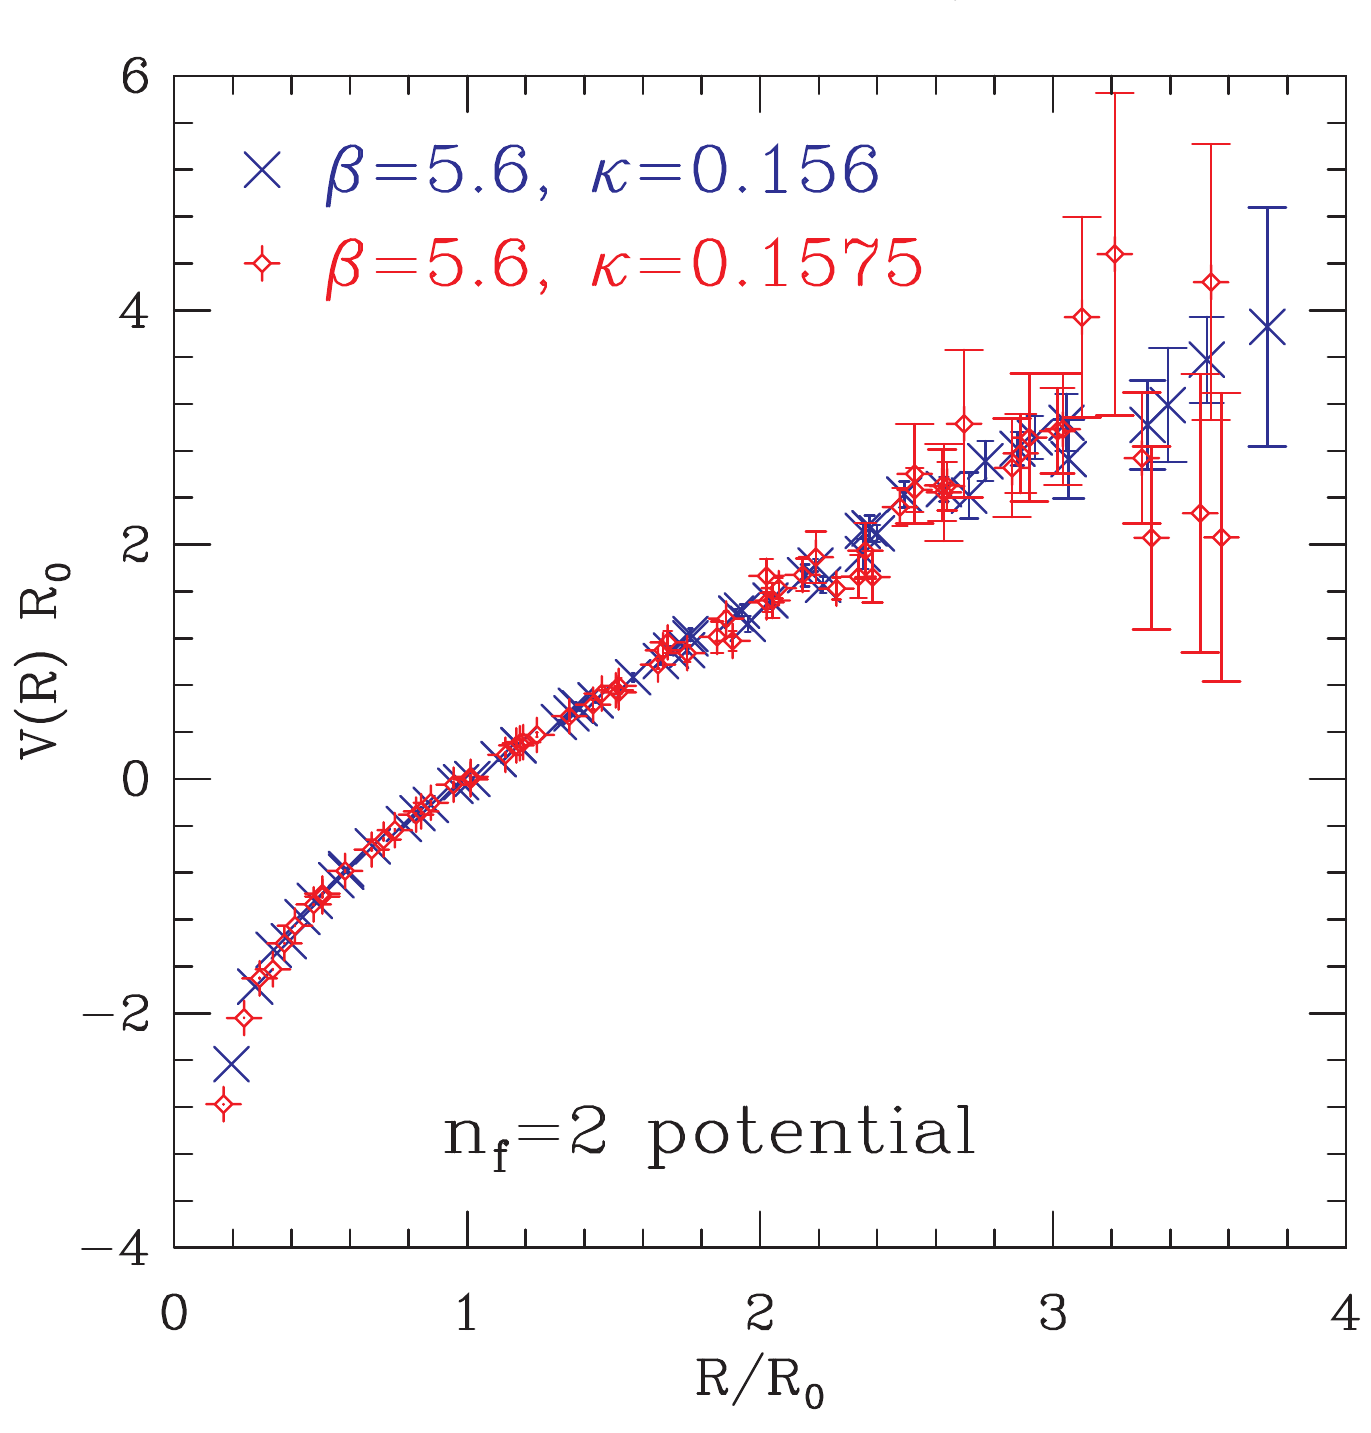
\includegraphics[width=0.8\textwidth]{images/fig11.png}
  \caption{The static $qq$ potential with two flavors of dynamical
    fermions obtained by the Wuppertal collaboration [119]. The dynamical
    quark mass in the $\beta = 6.0$, $\kappa = 0.156$ simulation is
    $\sim 2 m_s$ while that at $\kappa = 0.1575$ is $\sim m_s$. The rest is
    same as in Fig.~\ref{fig:10}. These data lie lower than the quenched
    points, however, for these dynamical quark masses there is no evidence
    yet of string breaking at large $R$.}
  \label{fig:11}
\end{figure}

The Cornell and Richardson potentials, which have been very successful in
predicting levels of charmonium and Upsilon system, yield
\begin{equation}
  R_0 \approx 0.49~\text{fermi}
  \label{eq:R0}
\end{equation}
Setting the scale using $R_0$ has the following advantages: (i) its value
is not very sensitive to the choice of the phenomenological potential,
(ii) it is defined at an intermediate distance where phenomenological
potentials are highly constrained by the $cc$ and $bb$ spectra,
(iii) lattice measurements of $V(R)$ at these intermediate distances can be
obtained with high precision, and (iv) this construction is valid for both
full and quenched QCD. The status of the current quenched data from three
collaborations is shown in Fig.~\ref{fig:12}. The data agree, and it turns
out that over this same range of $\beta$ the relation $R_0 = 1.18/\sqrt{\sigma}$
holds to a very good approximation. (The $\sigma$ is extracted from the
large $R$ behavior of the $qq$ potential as discussed above.) Thus, in
subsequent analyses of lattice data I will assume this relation when using
either $\sigma$ or $R_0$ to set the scale.

\begin{figure}[htbp]
  \centering
  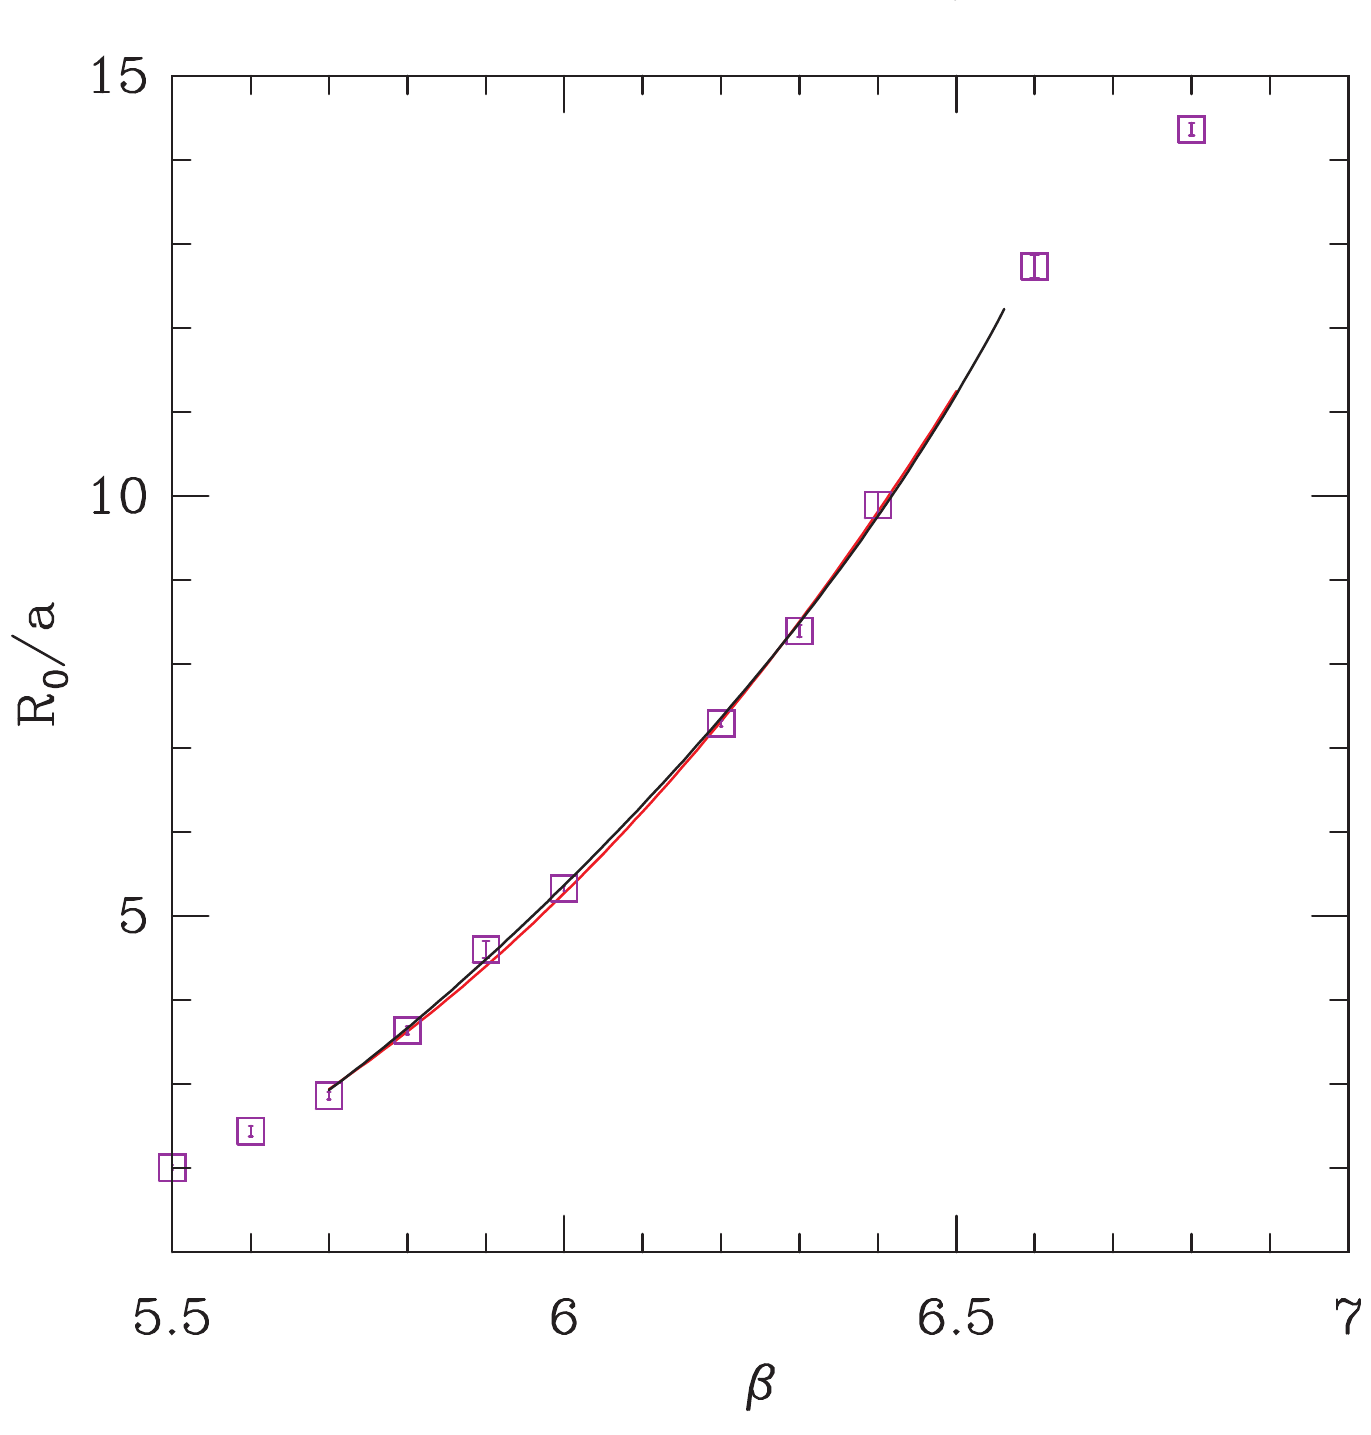
\includegraphics[width=0.8\textwidth]{images/fig12.png}
  \caption{The scale $R_0$ extracted from the static $qq$ potential. The
    data in purple are from [118,119,121] and the red line is a fit to
    these data. The black line is the fit
    $\log(a/R_0) = -1.6805 - 1.7139(\beta - 6) + 0.8155(\beta - 6.0)^2
    - 0.6667(\beta - 6)^3$ to the data by the Alpha collaboration [122].}
  \label{fig:12}
\end{figure}

For full QCD, the linear rising potential is screened. The string between
the $qq$ breaks when the energy is large enough to pop an additional $qq$
out of the vacuum and create two mesons. This phenomena of screening can
be tested by plotting $V(R)$ for different values of the dynamical quark
mass and observing the flattening of the linear rise. The value of $R/R_0$
at which the flattening should occur should decrease with $m_q$. A recent
analyses, again by the Wuppertal collaboration, is shown in
Fig.~\ref{fig:11} [119]. The data show no flattening---presumably because
the sea quark masses used in the update are not light enough to cause
string breaking at these $R/R_0$.

\subsection{Strong Coupling Expansion}
\label{sec:strong-coupling}

Confinement, for $\beta \to 0$, can be demonstrated using strong coupling
expansions. I will illustrate this technique by two examples---string
tension and the $0^{++}$ glueball mass.

The strong coupling expansion for SU($N$) gauge theory depends on the
following identities for integration over link matrices
\begin{align*}
  \int dg &= 1, &
  \int dg\, U_{ij} &= 0, &
  \int dg\, U_{ij}^\dagger &= 0, \\
  \int dg\, U_{ij} U_{kl} &= 0, &
  \int dg\, U_{ij}^\dagger U_{kl}^\dagger &= 0, &
  \int dg\, U_{ij} U_{kl}^\dagger &= \frac{1}{N}\delta_{il}\delta_{jk}
\end{align*}
\begin{equation}
  \int dg\, U_{i_1 j_1}\cdots U_{i_N j_N}
    = \frac{1}{N}\epsilon_{i_1\cdots i_N}\epsilon_{j_1\cdots j_N}.
  \label{eq:group-int}
\end{equation}
The essential point is that the group integration gives a non-zero result
only if each link occurs in a combination from which a color singlet can be
formed. Eq.~\eqref{eq:group-int} shows this for the identity, ``meson'' and
``baryon'' configuration of links.

The expectation value of the Wilson loop, at small $\beta$ (large $g$) for
the plaquette action, can be expanded as follows.
\begin{equation}
  \begin{aligned}
    W_{RT} &= \frac{1}{Z}\int dU\, W_{RT}\,
      e^{(\beta/2N)(W_{11}^{+}+W_{11}^{-})} \\
    &= \frac{1}{Z}\int dU\, W_{RT}\left[1 + \frac{\beta}{2N}\left(W_{11}^{+}
      + W_{11}^{-}\right) + \ldots\right]
  \end{aligned}
  \label{eq:W-expansion}
\end{equation}
where $W_{11}^{+}$, $W_{11}^{-}$ are the two orientations of the plaquette
and the trace over color incides in each loop is implicit. An inspection of
Fig.~\ref{fig:13}A shows that the first non-zero contribution to the
integral occurs when the loop $W_{RT}$ is tiled by elementary plaquettes
with the right orientation. Each such plaquette brings a factor of
$\beta/2N$ from the expansion and another factor of $1/N$ from the
integration. (Note that SU(2) is special and the combined factor is
$\beta/N^2$ as the two orientations of the loop have the same value, i.e.\
the trace is real.) Thus
\begin{equation}
  W_{RT} = \left(\frac{\beta}{2N^2}\right)^{RT}\left(1 + \ldots\right)
  \label{eq:W-area}
\end{equation}
where the leading corrections come from replacing any given tile with a
pillbox. Now using Eqs.~\eqref{eq:wilson-exp} and \eqref{eq:cornell} gives
\begin{equation}
  \sigma = -\log\frac{\beta}{2N^2} + O(\beta).
  \label{eq:sigma-sc}
\end{equation}
Thus all gauge theories, including U(1), confine in the strong coupling
limit. What distinguishes U(1) from non-abelian gauge theories is that the
U(1) gauge theory has a phase transition at $g^2 \sim 1$ (see
Section~15), and the physical theory
(electrodynamics) lies in the weak coupling region which is analytically
disconnected from the confining strong coupling limit.

As a second application of the strong coupling expansion consider the
calculation of $0^{++}$ glueball mass. The minimum tiling of the connected
plaquette-plaquette correlation function is the rectangular tube consisting
of four sides of size $1 \times T$ as shown in Fig.~\ref{fig:13}B. Thus
\begin{equation}
  W_{11}(T)W_{11}(0) \sim e^{-M_{0^{++}}T}
    = \left(\frac{\beta}{2N^2}\right)^{4T}\left(1 + \ldots\right),
  \label{eq:glueball}
\end{equation}
and
\begin{equation}
  M_{0^{++}} = -4\log\frac{\beta}{2N^2} + \ldots .
  \label{eq:Mglueball}
\end{equation}
The fact that the lowest order result $M_{0^{++}}/\sqrt{\sigma} = 4$ is very
close to present day estimates (see Section~18.3) is fortuitous.

\begin{figure}[htbp]
  \centering
  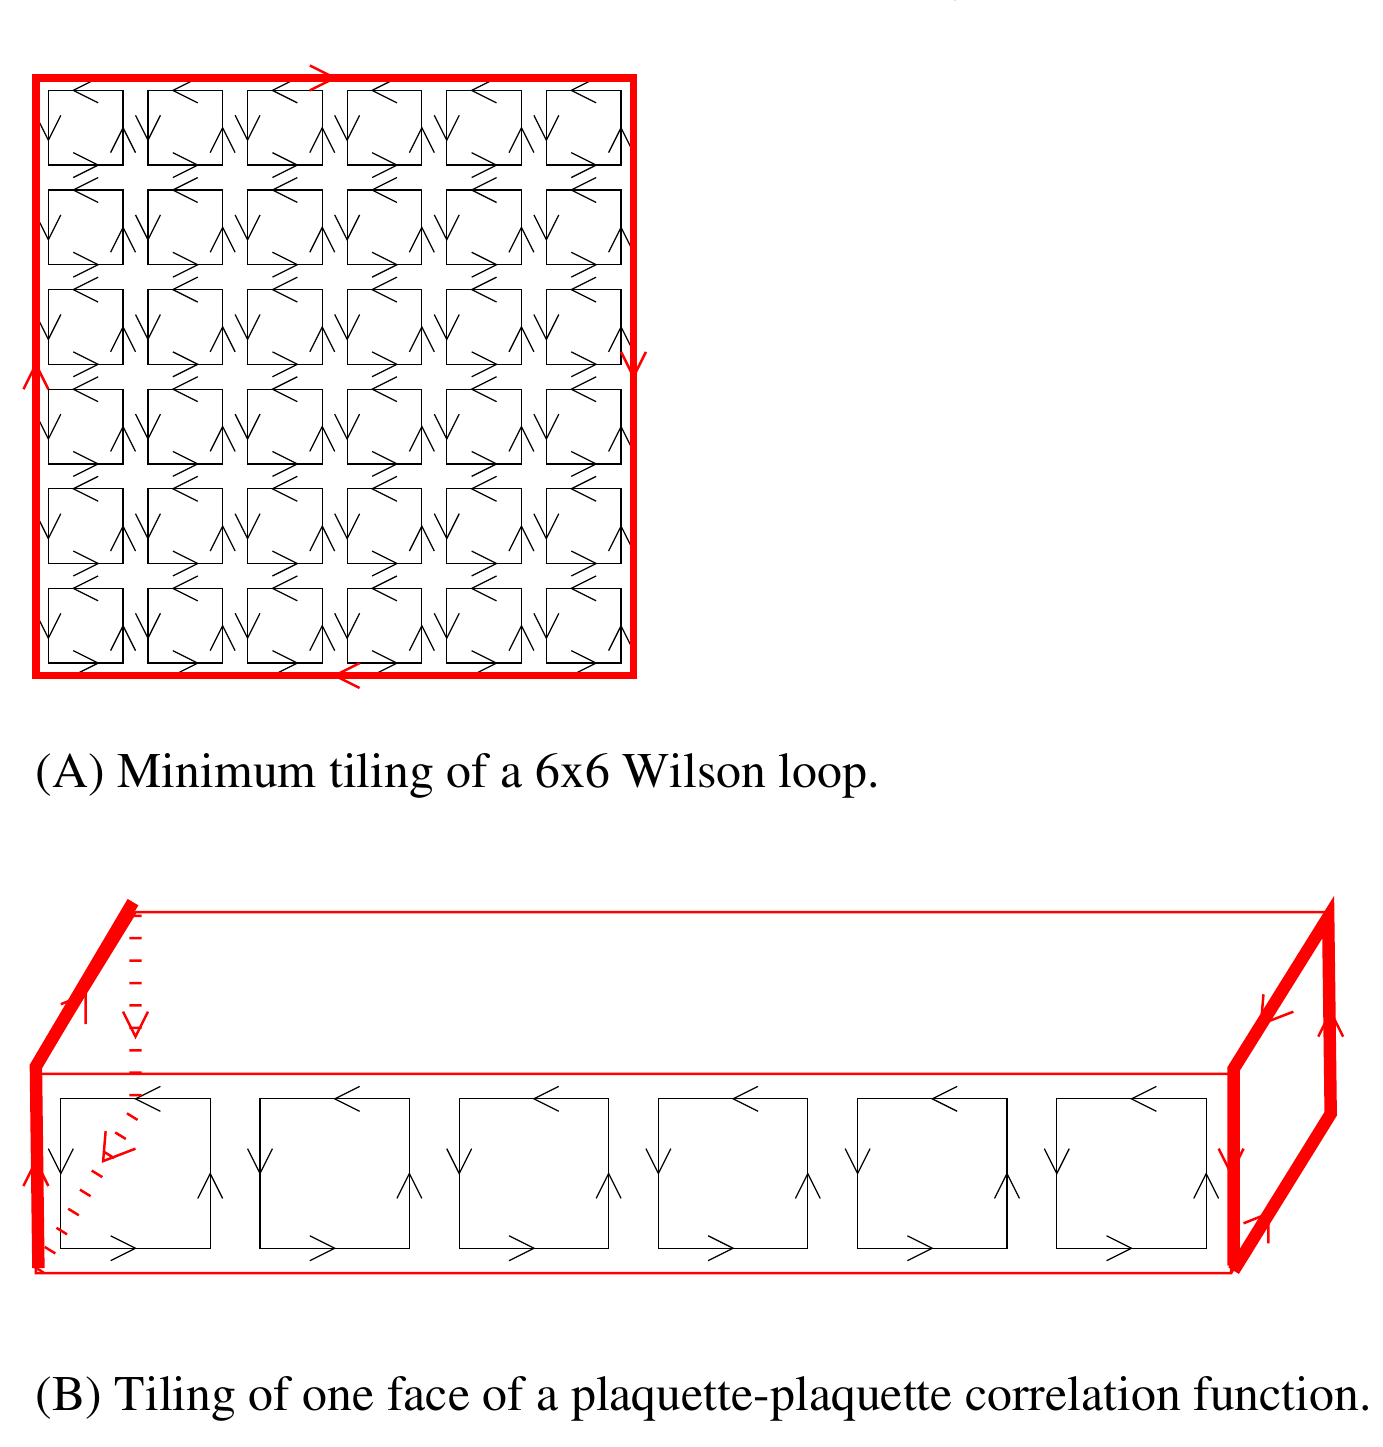
\includegraphics[width=0.8\textwidth]{images/fig13.png}
  \caption{Examples of minimum tiling of (A) a $6 \times 6$ Wilson loop,
    and (B) the plaquette-plaquette correlation function.}
  \label{fig:13}
\end{figure}

\textbf{Exercise:} What is the minimal tiling for the $0^{++}$ correlation
function built out of a $R \times R$ Wilson loop. Show that
Eq.~\eqref{eq:glueball} holds independent of the size of the loop.

\subsection{Wilson/Polyakov Line}
\label{sec:wilson-polyakov-line}

The Wilson line, pointing in say the time direction, is defined by the path
ordered product
\begin{equation}
  \langle L(x,y,z)\rangle = \mathrm{Tr}\, P \prod_{t=1}^{N_T}
    U_4(x,y,z,t)
  \label{eq:polyakov}
\end{equation}
It is gauge invariant due to periodic boundary conditions on gauge fields,
$U_4(x,y,z,N_T+1) = U_4(x,y,z,1)$. Repeating the above arguments made for
the Wilson loop one finds that the free energy of an isolated quark is
given by the Wilson/Polyakov line
\begin{equation}
  \langle L\rangle \sim e^{-F_q N_T}.
  \label{eq:free-energy}
\end{equation}
Thus, the possibility of having isolated charges in the theory requires
$F_q$ be finite.

In addition to gauge invariance, SU($N$) gauge theories have a global
$Z(N)$ invariance. It consists of multiplying all links on a given time
slice by the same element $z$ of $Z(N)$ without changing the action. Under
this transformation $\langle L\rangle \to z\langle L\rangle$. Such a global
symmetry can be spontaneously broken. Thus we have two possibilities
\begin{equation}
  \begin{array}{lll}
    \text{Broken:} & \langle L\rangle \neq 0 & \text{Deconfined}\ (F_q\ \text{finite}) \\
    \text{Unbroken:} & \langle L\rangle = 0 & \text{Confined}\ (F_q\ \text{infinite})
  \end{array}
  \label{eq:order-param}
\end{equation}
Thus, $\langle L\rangle$ is an order parameter, and tests for confinement
in pure gauge theories. It is also used to probe the location and order of
the finite temperature transition---a discontinuity in $\langle L\rangle$
signals a first order transition, whereas a continuous change implies
second order.

Svetitsky and Yaffe [128] argued that for the purposes of determining the
order of the finite temperature transition the relevant effective theory is
a 3-dimensional spin model of short-ranged interactions (between Wilson
lines reduced to spin variables) with a $Z(N)$ symmetry. Then using the
universality classes known from renormalization group analyses, they
predicted that the transition for SU(2) should be second order (Ising
class), whereas for SU($N \geq 3$) it should be first order (P\"otts
class). Numerical results are consistent with these predictions, in
particular for SU(2) the critical exponents have been determined using
standard techniques of Statistical Mechanics and found to agree with those
of the 3-dimensional Ising model [129].

In the presence of dynamical quarks, it is easy to see that the discretized
Dirac action is not invariant under the $Z(N)$ symmetry. Consequently,
$\langle L\rangle \neq 0$ for all values of $\beta$, so $\langle L\rangle$
is no longer an order parameter. Nevertheless, changes (discontinuous or
continuous) in it are used to search for the location of the finite
temperature phase transition and its order.

% SECTION 15: Phase Transitions in the Lattice Theory
% Source: extract/sec15.txt (PDF pages 93-97) + continuation at the head of
% extract/sec16.txt (PDF page 98, before the "16. Errors in Lattice Results" heading).

\chapter{Phase Transitions in the Lattice Theory}

The lattice theory with a finite cut-off $\mu = \pi/a$ can be regarded as an effective theory. The integration over momenta in the range $\{\pi/a, \infty\}$ renormalizes the couplings and generates additional effective interactions (see Section 8 and the lectures by M.~L\"uscher for a detailed discussion of this approach). Thus, one can regard the lattice theory as a point in an infinite dimensional space of couplings, and taking the continuum limit as a flow in this space to the critical point at $a = 0$ that defines the physical theory. In this way of thinking about LQCD as a Statistical Mechanics system one is automatically lead to the questions
\begin{itemize}
\item What is the phase diagram in this extended coupling constant space?
\item Are there other fixed points, and if so what is the nature of the theory at those points?
\item What are the order parameters that characterize different phases?
\end{itemize}

The starting point of my discussion of these questions will be the pure gauge theory. As before, the generalized form of the gauge action is
\begin{equation}
S_g = \beta \sum_{i,j} \sum_{\mu,\nu} \sum_x c_{i,j}\, \mathrm{Re}\, \mathrm{Tr}\, W^{i,j}_{\mu\nu}
\end{equation}
where the sum over $i$ in $W^{i,j}_{\mu\nu}$ is over all possible Wilson loops and $j$ is over all representations of the loop. $\beta$ is the overall coupling and the $c_{i,j}$ give the relative strengths of the different loops.

The three simplest gauge invariant probes of the phase diagram are (gauge non-invariant quantities have zero expectation values as shown by Elitzur [37])
\begin{itemize}
\item Wilson loops: These, as discussed in Section 14.2.1, contain information on the potential between static quarks.
\item Wilson/Polyakov lines. These measure the free energy of an isolated quark.
\item The chiral condensate $\langle \bar{\psi}\psi\rangle$. This provides information on vacuum alignment under spontaneous chiral symmetry breaking.
\end{itemize}

LQCD, in the limit $g \to \infty$, can be analyzed using strong coupling expansions as discussed in Section 14.2.2. Using these it was shown that, in the limit $g \to \infty$, the expectation value for Wilson loops has an area law for all gauge groups ($U(1)$ and $SU(N)$). Since electrodynamics ($U(1)$) does not confine, this region of coupling space cannot correspond to the physical theory. In other words, there should exist a phase transition separating the strong coupling and weak coupling phases of non-confining theories like $U(1)$. This has been established for $U(1)$, both analytically [130] and by Monte Carlo simulations [131]. For a theory like QCD, with both confinement and asymptotic freedom, we need to know if the two regions of parameter space are analytically connected. Analytical methods like strong and weak coupling expansions can be used provided the range of validity of the expansions gives a sufficiently large overlap, otherwise non-perturbative methods are necessary.

To address these questions for $SU(3)$ I show, in Fig.~\ref{fig:14}, the behavior of square loops, $\{\mathrm{Re}\,\mathrm{Tr}\, W^{i \times i}\}$, as a function of the coupling $\beta$ for the simplest action---Wilson's plaquette action. Also shown for comparison are the strong coupling expansion to $O(\beta^5)$ [133], the weak coupling expansion to $O(g^4)$ [134] and its tadpole improved (TIPT) version. These numerical data show that there is a smooth though sharp transition between the weak coupling and strong coupling phases, i.e.~no phase transitions. The crossover takes place in the window $5 \lesssim \beta \sim 6$, with the larger loops becoming perturbative at slightly higher $\beta$. Both strong coupling and weak coupling expansions fail in this region (for TIPT this is evident only for large loops), so numerical methods are essential. Such an analysis was the basis of the pioneering work of Creutz, and Creutz, Jacobs, and Rebbi [132], who showed that the string tension changes from its strong to weak coupling behavior without a phase transition. Their calculations yielded the first clue that it may be possible to get continuum physics with $O(20\%)$ errors from simulations at $\beta \gtrsim 6.0$.

\begin{figure}[htbp]
\centering
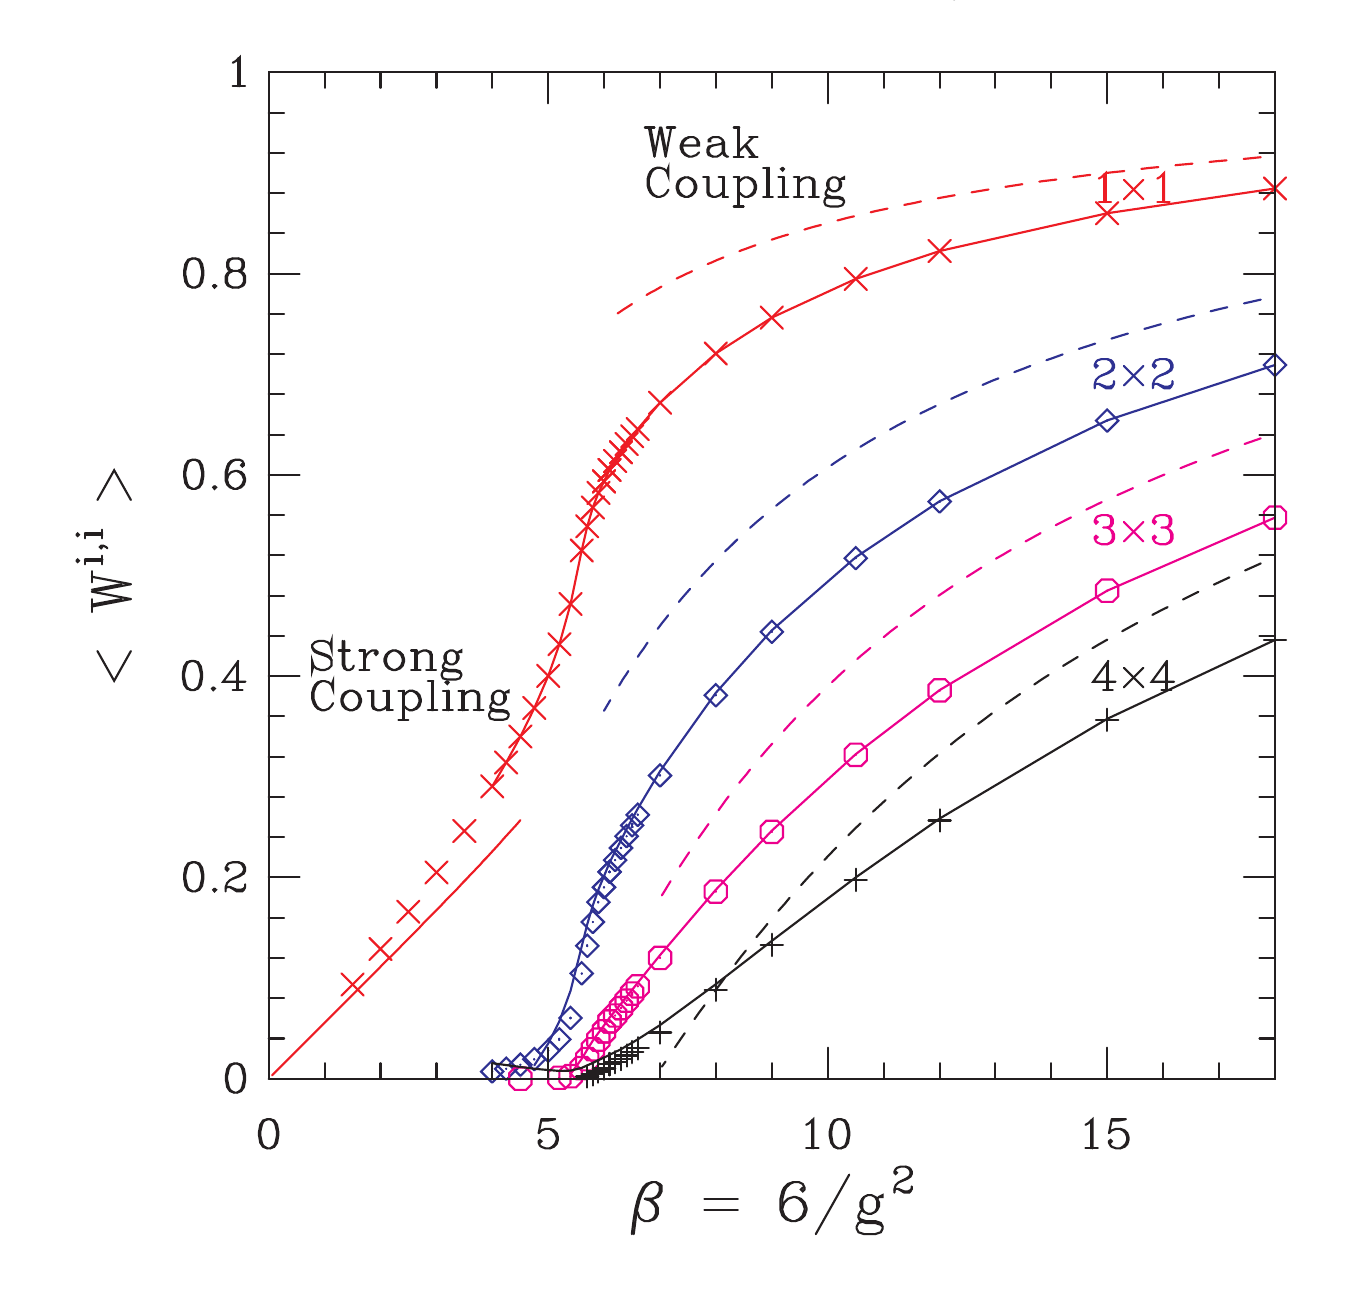
\includegraphics[width=0.8\textwidth]{images/fig14.png}
\caption{The behavior of the expectation value of square Wilson loops as a function of coupling $\beta$. The data, show a sharp crossover between $5 \lesssim \beta \lesssim 6.0$. Result of the strong coupling expansion to $O(\beta^5)$ and weak coupling expansion to $O(g^4)$ are shown by the dashed line. Results of tadpole improved weak coupling expansion (TIPT) are shown by the solid lines. Since the improved coupling is defined in terms of the $1 \times 1$ loop, $g_I^2 = g^2/\langle W^{1 \times 1}\rangle$, the agreement between the data and TIPT is a trivial result of the construction as explained in the text. The improvement in larger loops, however, demonstrates the efficacy of TIPT.}
\label{fig:14}
\end{figure}

The TIPT result shown in Fig.~\ref{fig:14} is obtained as follows. The mean-field improved Wilson loop expectation value is defined to be
\begin{equation}
\langle W^{i \times i}\rangle = \langle \tilde{W}^{i \times i}\rangle\, u_0^{4i},
\end{equation}
where for $u_0$ I use the non-perturbative value obtained from the plaquette as it is more readily available. The improved expansion for $\langle \tilde{W}^{i \times i}\rangle$, after absorbing the tadpoles using the plaquette, is given by
\begin{equation}
\langle \tilde{W}^{i \times i}\rangle = \frac{\langle W^{i \times i}\rangle}{\langle W^{1 \times 1}\rangle^i},
\end{equation}
where both terms on the right are first expanded in terms of $\tilde{g}^2 = g^2/u_0^4(\mathrm{pert}) = g^2/\langle W^{1 \times 1}\rangle_{\mathrm{pert}}$ to order $\tilde{g}^4$, and then the ratio is truncated at order $\tilde{g}^4$. It is obvious that using $u_0$ from the plaquette guarantees a perfect fit for $\langle W^{1 \times 1}\rangle$, however the improvement in even the $\langle W^{4 \times 4}\rangle$, is remarkable.

The first study of the phase diagram in the generalized coupling constant space was done using an action constructed from the plaquette in both the fundamental and adjoint representations of the $SU(N)$ gauge theory [135]
\begin{equation}
S = \beta_F \sum_x \frac{1}{N} \mathrm{Re}\, \mathrm{Tr}\, W_{1 \times 1} + \beta_A \sum_x \frac{1}{N^2} |\mathrm{Tr}\, W_{1 \times 1}|^2 .
\end{equation}
For this action, the effective bare coupling, obtained using a Taylor expansion, is
\begin{equation}
\beta_{\mathrm{eff}} \equiv \frac{2N}{g_{\mathrm{eff}}^2} = \beta_F + 2\beta_A .
\end{equation}
Thus simulations can be done in the negative $\beta_A$ region as long as $\beta_F > 2|\beta_A|$. This is a classical condition that avoids the weak coupling singularity.

The resulting lines of first order bulk transitions, along with the location of the end point for three gauge groups, are show in Fig.~\ref{fig:15}. The point at $\beta_A = \infty$ is the first order transition in the $Z(N)$ gauge theory, while that at $\beta_F = 0$ corresponds to that in the $SO(N)$ theory. The location of the third end-point with respect to the $\beta_F$ axis depends on $N$. Current estimates of the location are [136--138]
\begin{equation}
\begin{array}{lll}
\beta_F = 1.22 & \quad \beta_A = 1.25 & \quad \mathrm{SU}(2) \\
\beta_F = 4.00(7) & \quad \beta_A = 2.06(8) & \quad \mathrm{SU}(3) \\
\beta_F \sim 12{-}15 & \quad \beta_A = (-1) - (-5) & \quad \mathrm{SU}(4)
\end{array}
\end{equation}

The fact that for $N \le 3$ this point lies above the $\beta_F$ axis is consistent with the observation that there is no discontinuity in the behavior of Wilson loop data as show in Fig.~\ref{fig:14}. If one were to take the continuum limit along a line crossing the transition line above this point, for example along the dotted line $A$ in Fig.~\ref{fig:15}, then there would be discontinuities in Wilson loops (and consequently in the string tension), specific heat, and glueball masses at the point of intersection with the transition line. At the end-point $X$ the specific heat diverges and consequently the $0^{++}$ glueball mass goes to zero. (Note that the specific heat is the volume integral of the $0^{++}$ glueball correlation function with the plaquette as the interpolating operator. Thus the divergence in the specific heat implies a zero in the $0^{++}$ glueball mass.) The string tension and masses of glueball states with other spin-parity quantum numbers are non-zero and continuous at this point. Such phase transitions are lattice artifacts. For example, taking the continuum limit at $X$, i.e.~setting $a = 0$, would give a free theory as all states other than the $0^{++}$ glueball become infinitely heavy.

\begin{figure}[htbp]
\centering
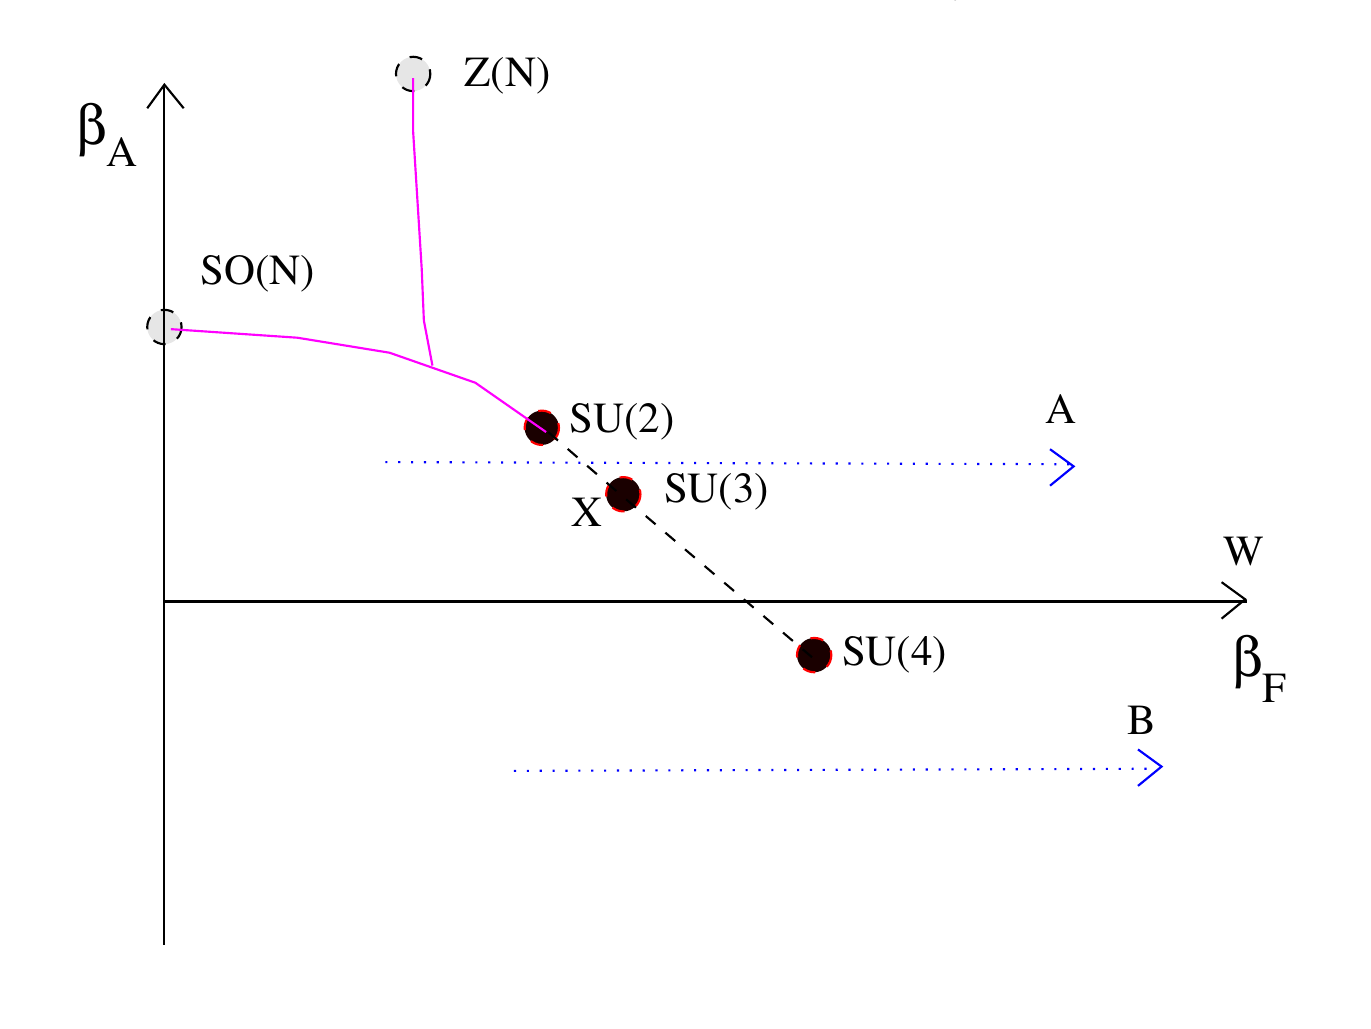
\includegraphics[width=0.8\textwidth]{images/fig15.png}
\caption{The phase diagram of $SU(N)$ gauge theories in the fundamental-adjoint coupling constant space.}
\label{fig:15}
\end{figure}

One can take the continuum limit for the $SU(3)$ gauge theory along any trajectory like $A$ or $W$ or $B$. In case $A$ it is necessary to keep $\beta_F > \beta_F^*$ to avoid the lattice artifacts. Along $W$, while there are no singularities, the artifact $X$ could, around $\beta_F = 5.7$, cause significant deviations from the physics of the relevant fixed point at $g = 0$. Lattice data verify this scenario---the non-perturbative $\beta$-function measured from observables other than $M_{0^{++}}$ shows a large dip around $\beta_F = 5.7$ [89]. Thus, to avoid these artifacts requires simulations for $\beta_F \gtrsim 6.0$. On a trajectory like $B$ the influence of $X$ is expected to be less than along $W$, and it is possible that contact with continuum physics can be made on coarser lattices. If so then the trajectory $B$ corresponds to an ``improved action'' in accordance with the third criteria enumerated in Section 8.

This qualitative argument for taking the continuum limit along a trajectory like $B$ is supported by Monte Carlo renormalization group (MCRG) estimates of the renormalized trajectory [87]. Such calculations of the RT yield a negative value for $\beta_A$. As explained above, the most sensitive probe of the expected improvement on including a $\beta_A$ term in the action, is the behavior of $M_{0^{++}}$. Until recently tests of this conjecture were limited by statistical accuracy [166]. The recent calculations on anisotropic lattices of glueball spectra by Morningstar and Peardon [139] validate this scenario. I shall discuss their results in Section 18.3.

It is clear that there are additional phase transitions in the generalized lattice theory. For example one would get a similar diagram to that in Fig.~\ref{fig:15} if the action was defined in terms of the $1 \times 2$ loop in the fundamental and adjoint representations. The question, therefore, is whether there exist other second order transition points at which all correlation lengths (measured in lattice units) diverge i.e.~where a non-trivial continuum limit exists. The commonly held belief, supported by numerical data, is that all such points lie on the hypersurface defined by $g_{\mathrm{eff}} = 0$. The long distance behavior of these theories is controlled by the fixed point defined with respect to a suitable renormalization group transformation. Taking the continuum limit of the lattice theory on this hypersurface provides a non-perturbative definition of QCD. This is the standard scenario.

An alternative scenario is the presence of a non-trivial fixed point at $g_{\mathrm{eff}} \neq 0$ [140]. If this unlikely possibility turns out to be true then the perturbative relation between $g_{\mathrm{eff}}$ and $a$, based on asymptotic freedom, would change---the coupling would no longer run to zero as the momentum scale $Q \to \infty$. This could be exposed by precise measurements of $\alpha_s$ as a function of $Q^2$, or by a detailed search for non-trivial second order phase transitions in the lattice theory.

In either case the non-perturbative lattice analyses of quantities such as the spectrum and weak matrix elements does not change. To get to the continuum limit we would still extrapolate the lattice data in $a$ to $a = 0$. Only the PQCD relation between $a$ and $g$ would be invalid, consequently extrapolations using the perturbative scaling relation could not be used.

My bottom line on this issue, having mentioned the heretical view, is to proceed assuming that the standard scenario is correct.

% SECTION 16: Errors in Lattice Results
% Source: extract/sec16.txt (PDF pages 98-107), from the "16. Errors in Lattice
% Results" heading to the end of the extract. The extract ends mid-sentence
% ("...extrapolate keeping only the terms in"); the closing sentence and the
% final paragraph of Section 16 (which fall at the top of extract/sec17.txt,
% PDF page 108) are completed from the author's original source
% (chap-errors.tex) so the chapter is complete.

\chapter{Errors in Lattice Results}

Numerical simulations of lattice QCD introduce both statistical and a number of systematic errors. I have collected together a brief description of the various errors here, and in the remainder of the article I will only give quantitative estimates. I will label a particular systematic uncertainty as negligible/important if it is negligible/comparable in magnitude to the statistical error for that observable as determined in a state-of-the-art calculation.

\section{Statistical errors}

The monte carlo method for doing the functional integral employs statistical sampling. The results, therefore, have statistical errors. The current understanding, based on agreement of results from ensembles generated using different update algorithms, different initial starting configuration, and different random number generators in the Markov process, is that the functional integral for QQCD is dominated by a single region. Second, we find that configurations with non-trivial topology are properly represented in an ensemble generated using a Markov chain based on small changes to link variables. Based on these observations we conclude that the energy landscape is simple, consequently, the statistical errors should fall as $1/\sqrt{N}$, where $N$ is the number of independent measurements. Tests like binning of the data and the calculation of auto-correlation times for various observables are used to determine the monte-carlo time between independent configurations.

Estimates of decorrrelation times in dynamical simulations are just becoming available and the understanding of decorrelation times for various update algorithms and different fermion formulations is not complete. A recent study of decorrelations for update of Wilson fermions [142] using the hybrid Monte Carlo algorithm [141] (the algorithm of choice) presented very encouraging results. They found that decorrelation time based on tunneling rate between different topological sectors (expected to be amongst the slowest modes) was within a factor of two of standard probes like large Wilson loops and hadron correlators, and $\approx 80$ units of molecular dynamics time for $m_\pi / M_\rho \ge 0.56$. Thus trajectory lengths of 5000--10000 units, which are feasible on todays computers, provide a reasonable statistical sample. Even though details like how this decorrelation time grows with decreasing quark mass still need to be filled in, it is clear that current Monte Carlo algorithms do provide a reliable way of doing the functional integral for both QQCD and full QCD.

\section{Finite Volume}

This is the simplest error to visualize as it is associated with using finite lattices to represent an infinite system. L\"uscher has shown that for sufficiently large lattices of side $L$, the finite volume corrections in the mass $M$ of a given state fall off as $e^{-ML}$ [27]. This anaylsis assumes that the interactions with the mirror states on a periodic lattice are small. On small lattices the wave-function of the states is squeezed, resulting in an much more rapid increase of the mass with decreasing lattice size. This effect is seen clearly for $L < 1.5$ fermi, where the finite size behavior fits a power-law, $\sim 1/L^3$ [143]. The goal, therefore, is to work on lattices large enough such that the finite size effects are exponentially suppressed.

To determine the lattice size needed for observables involving quark propagation I choose the pion as the test state as it the lightest and thus has the largest correlation length. Results of quenched simulations show that for $M_\pi L \ge 5$ the exponential suppression applies and the corrections are negligible. For physical value of $M_\pi$ this translates into $L \ge 7$ fermi. Another way of stating the same criteria is that the quantum mechanical properties of hadrons, typically of size $\le 1$ fermi, are unaltered if the box size is larger than $7$ fermi. Current simulations explore quark masses in the range $m_q \ge m_s/4$ or equivalently $M_\pi / M_\rho \ge 0.4$. For these ``heavier masses'' the criteria $M_\pi L \ge 5$ translates into $L \ge 3$ fermi. The lattices used in the most recent calculations, for example the CP-PACS runs, discussed later, satisfy this condition.

Another consequence of finite $L$ is momentum resolution. For example, the lowest non-zero momentum, and spacing, is $2\pi/La = 393$ MeV for $L = 32$ and $1/a = 2$ GeV. One would like a much finer resolution when investigating the dispersion relation for mesons and baryons or when calculating matrix elements required to study form-factors in semi-leptonic and rare decays. This can only be done by increasing either $L$ or $a$. Increasing $L$ is limited by computer resources, while increasing $a$ increases discretization errors which are discussed next.

\section{Finite lattice spacing errors}

The lattice is merely a technical scaffold and the physical results are obtained by taking the $a \to 0$ limit. At finite $a$, lattice results have discretization errors whose size depend on the degree to which the lattice action and operators have been improved (see Sections 8, 12, and 13). As discussed in Section 8, we employ two strategies for removing these errors. First, improve the lattice action and operators so that the errors at fixed $a$ are small, and secondly, repeat the simulations at a number of values of $a$ and extrapolate to $a = 0$. Since the functional form used to characterize the errors is usually truncated to just the leading term in $a$, the extrapolation has an associated systematic error. To get a handle on this uncertainty, extrapolations have been done for three different formulations (Wilson, clover, staggered) for which the leading corrections are different ($O(a)$, $O(\alpha a) - O(a^2)$, $O(a^2)$). The difference between the three results in the $a = 0$ limit is a measure of the residual uncertainty. I shall illustrate this procedure for controlling the discretization errors in Section 20 where the calculation of quark masses is discussed.

\section{Chiral Extrapolations in the light quark masses}

The physical $u$ and $d$ quark masses are too light to simulate on current lattices. For $1/a = 2$ GeV, realistic simulations require $L/a \gtrsim 70$ to avoid finite volume effects, i.e.~keeping $M_\pi L \ge 5$. Current biggest lattice sizes are $L/a = 32$ for quenched and $L/a = 24$ for unquenched. Thus, to get results for quantities involving light quarks, one typically extrapolates in $m_u = m_d$ from the range $m_s/4 - 2m_s$ using functional forms derived using chiral perturbation theory but truncated to the first couple of terms. Since the range of the chiral extrapolation is large, it is important to quantify the size of the higher order chiral corrections. This requires precise data at a large number of values of quark masses. Most of the current fits are based on keeping just the lowest order terms as the quality of the data is not good enough to quantify the various higher order corrections, and/or to identify the quenched artifacts discussed in Section 16.8. The status of the current data with respect to resolving these higher order corrections is discussed in Section 18 where an analysis of $SU(3)$ flavor symmetry breaking, for example the mass differences between mesons and baryons within $SU(3)$ multiplets like the baryon octet and the decuplet, is presented.

Current simulations also neglect isospin breaking effects and electromagnetic contributions as these are a few MeV in nature, and smaller than the present numerical resolution. The iso-spin symmetric mass is defined by $\bar{m} = (m_u + m_d)/2$. For an exploratory analysis of iso-spin breaking effects in the presence of a strong $U(1)$ field see Ref.~[144].

I expect that our understanding of the chiral corrections will change significantly in the next two years due to the factor of 10--100 increase in the computational power made available to LQCD. To study iso-spin breaking effects properly requires dynamical lattices with roughly physical values for $m_u$ and $m_d$. Such simulations are still a few years away.

\section{Discretization of Heavy Quarks}

Simulations of heavy quarks ($c$ and $b$) have large discretization errors of $O(ma)$ in addition to the $O(\Lambda_{QCD}a)$ and $O(pa)$. This is because quark masses measured in lattice units, $m_c a$ and $m_b a$, are of order unity for $2\ \mathrm{GeV} \le 1/a \le 5\ \mathrm{GeV}$. Data show that these discretization errors are large even for $m_c$ in the case of Wilson and clover actions. (Staggered fermions do not have any advantage over Wilson-like discretizations for heavy quarks and are hence not used to study heavy quarks.) A number of alternate approaches are being investigated to address this issue (see Section 13). These include the non-relativistic QCD (NRQCD) formulation [108], lattice versions of the heavy quark effective theory [145], a variant of the Dirac discretization that interpolates between NRQCD and clover discretizations [113], and non-perturbatively $O(a)$ improved SW-clover fermions [104]. Many collaborations are testing these formulations, however, it is still too early to judge which approach will provide the best solution to the simulations of heavy quarks.

\section{Matching between lattice and continuum scheme (renormalization constants)}

Experimental data are analyzed using some continuum renormalization scheme like $\overline{MS}$ so, to make contact with phenomenology, results in the lattice regularization scheme have to be converted to the continuum scheme. The perturbative relation between renormalized quantities in $\overline{MS}$ and the lattice scheme are, in almost all cases, known only to 1-loop. Data show that the $O(\alpha_s)$ corrections can be large, $\sim 10 - 50\%$ depending on the quantity at hand. However, as explained by Parisi [77] and by Lepage and Mackenzie [78], these large corrections are mostly due to lattice artifacts which, once identified as coming from tadpole diagrams, can be removed. The Lepage--Mackenzie prescription for reorganizing the lattice perturbation theory to remove these artifacts has significantly reduced the associated uncertainty. Nevertheless, the improvement is not uniform and in many cases the corrections are still large, and the residual errors in TI 1-loop perturbative estimates are hard to ascertain. The final step in improving the reliability of the matching factors is to develop non-perturbative methods [146--148]. Significant progress has been made in setting up these calculations, and once they are complete the uncertainties in existing results due to using 1-loop $Z$'s will be removed. An illustration of the effect of using perturbative versus non-perturbative $Z$'s is presented in Section 20.1.

\section{Operator mixing}

As mentioned in Section 3, a major application of LQCD is to calculate the matrix elements of operators that arise in the effective weak Hamiltonian between hadronic states. In addition to the question of the overall normalization of these operators, the operators can, in general, mix with operators of the same, higher, and \textit{lower} dimensions. On the lattice this mixing arises due to quantum corrections and discretization errors. The set of lattice operators one has to consider is usually larger than those in the continuum theory because at finite $a$ the symmetries of the lattice theory are smaller than those of the continuum theory, for example the hard breaking of chiral symmetry in Wilson fermions. In cases where there is mixing with lower dimensional operators, the mixing coefficients have to be known very accurately otherwise the power divergences overwhelm the signal as $a \to 0$. Similarly, in cases where there is mixing with operators of the same dimension but with different tensor structures, as in Wilson-like actions due to the explicit breaking of chiral symmetry, the chiral behavior may again be completely overwhelmed by these lattice artifacts if the coefficients are not known precisely. Examples where such mixing has posed serious computational challenges are the matrix elements of 4-fermion operators needed in the calculation of the $\Delta I = 1/2$ rule, $B_K$, $B_6$, and $B_8$. In these cases also non-perturbative methods for calculating the mixing coefficients are essential. For a discussion of these methods see Prof.~Martinelli's lectures.

\section{Quenched Approximation (QQCD)}

This approximation is computationally the hardest to shed and quantify. Since it plays a key role in today's simulations, I will discuss it in some detail. The approximation consists of ignoring the fermion contribution to the path integral, i.e.~setting $\det M = \mathrm{constant}$ in Eq.~4.3. The sole reason for this approximation is limitations of computer power. With known algorithms the computational requirements of full QCD simulations go up by factors of $10^3 - 10^5$ depending on the quark mass. Since QQCD is confining, asymptotically free, and shows spontaneous chiral symmetry breaking ($\langle \bar{\psi}\psi\rangle_{QQCD} \neq 0$), and differs from full QCD only in the relative weighting of the background gauge configurations, the physics analyses are identical in most cases. It is therefore considered reasonable to do detailed quenched simulations in order to understand and control all other sources of errors while waiting for better algorithms or the computer technology needed to provide the required additional factor of $10^3 - 10^5$, i.e.~10--1000 teraflop capability.

\begin{figure}[htbp]
\centering
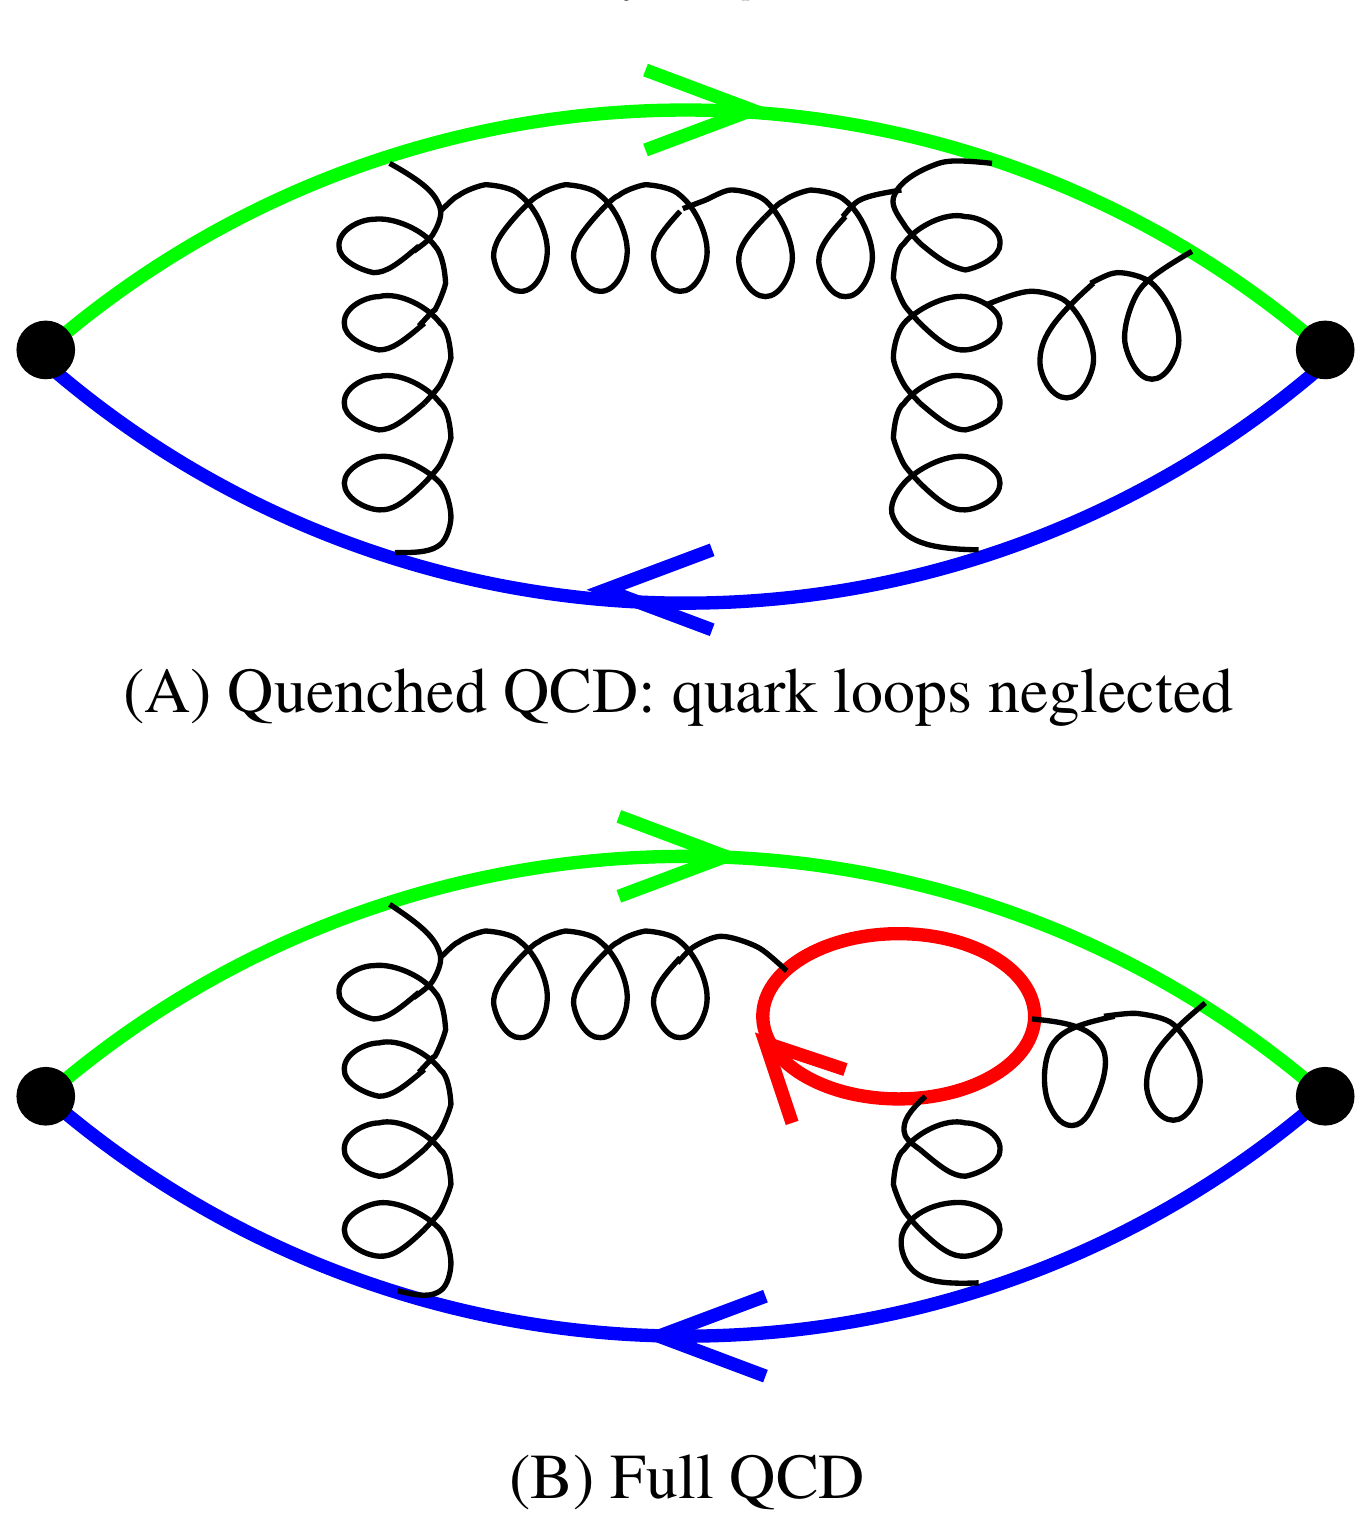
\includegraphics[width=0.8\textwidth]{images/fig16.png}
\caption{An illustration of the difference between quenched QCD and QCD. QQCD has no vacuum polarization loops on virtual gluon lines.}
\label{fig:16}
\end{figure}

Physically, the quenched approximation corresponds to turning off vacuum polarization effects of quark loops. This is illustrated in Fig.~\ref{fig:16} for the pion correlator. One important consequence of neglecting vacuum polarization effects is the behavior of the potential between a $q\bar{q}$ pair as a function of the separation. In the full theory the string breaks by the creation of a $q\bar{q}$ pair out of the vacuum, therefore at large distances there is a screened potential between two mesons. For such screened potential large Wilson loops should show a perimeter law. In QQCD the string does not break and large Wilson loops show an area law. Thus the long distance behavior of the two theories is very different and one might be led to believe that QQCD is a bad approximation. However, because of confinement, the long distance scale that is relevant to hadronic physics has a natural cutoff of a few fermi. Thus, if one can match the potential between some fine scale ($\sim 0.01$ fermi, below which asymptotic freedom makes the calculations perturbative) and the typical size of hadrons ($\sim 1$ fermi) then QQCD could give reasonable estimates for the hadronic spectrum. This argument is really only applicable to heavy onia, where potential models work well. For light quarks one simply has to do the simulations to estimate the size of the distortions. In any case the community has proceeded by assuming that the two theories can be roughly matched by adjusting the quenched coupling constant at some scale like $0.5$ fermi, or equivalently by adjusting the overall scale $\Lambda_{QQCD}$, and hopes that the quenching corrections are small, $10 - 20\%$, for many cases. If this bears out then even QQCD would yield many phenomenologically useful predictions.

In spite of the optimism, the fact remains that QQCD is not a unitary theory, so it is important to understand how it fails. I would like to illustrate its shortcomings with the following examples.

We can calculate the $\rho\pi\pi$ coupling in both QCD and QQCD by measuring the three point function $\langle T[\rho\pi\pi]\rangle$ illustrated in Fig.~\ref{fig:17}A. The difference between the two values is a measure of the validity of QQCD. On the other hand the diagram shown in Fig.~\ref{fig:17}B is absent in QQCD, and the $\rho$ spectral function does not have a cut beginning at $2M_\pi$. Thus, the $\rho\pi\pi$ coupling \textit{cannot} be extracted from an analysis of the $\rho$ 2-point function in QQCD.

\begin{figure}[htbp]
\centering
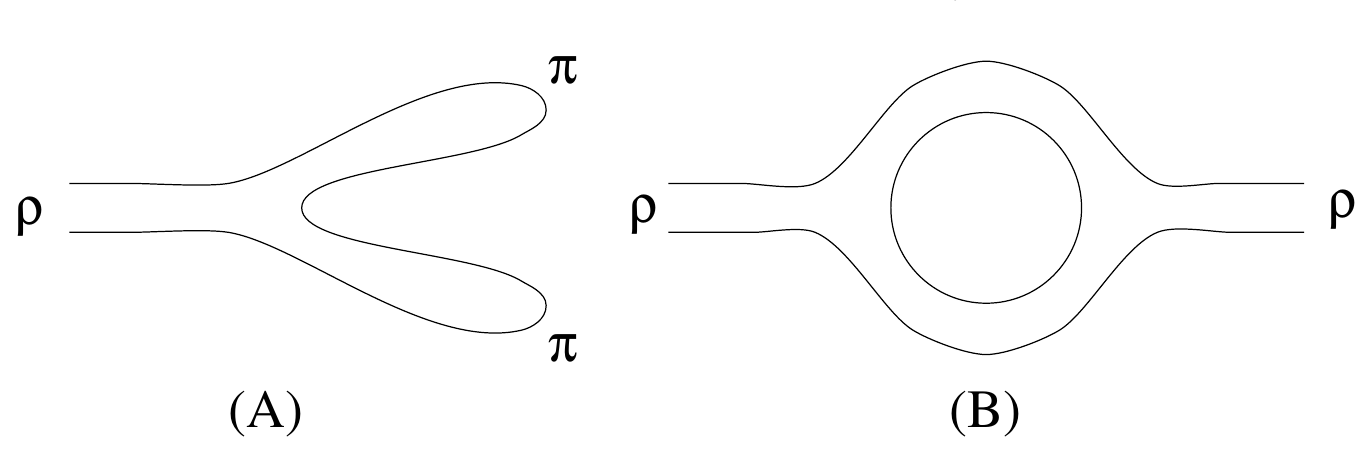
\includegraphics[width=0.8\textwidth]{images/fig17.png}
\caption{The $\rho\pi\pi$ coupling from the $\rho \to \pi\pi$ decay and (B) the $\rho$ correlator in full QCD.}
\label{fig:17}
\end{figure}

A very important difference between full QCD and QQCD is the behavior of the $\eta'$. In full QCD the singlet axial current is anomalous and the $\eta'$ acquires a large mass due to the summation of vacuum polarization graphs shown in Fig.~\ref{fig:18},
\begin{equation}
\frac{1}{p^2 - M^2} + \frac{1}{p^2 - M^2} M_0^2 \frac{1}{p^2 - M^2} + \cdots = \frac{1}{p^2 - M^2 - M_0^2}
\end{equation}
where, for simplicity I have approximated the gluonic coupling by a momentum independent constant $M_0^2$. This is related to the topological susceptibility via the Witten--Veneziano relation $M_0^2 = 2n_f \chi_t / f_\pi^2 = M_{\eta'}^2 + M_\eta^2 - 2M_K^2$ [149]. In QQCD the absence of the vacuum polarization diagrams means that the $\eta'$ propagator has a single and a double pole, i.e.~$(p^2 - M^2)^{-1}$ and the ``hairpin'' term $(p^2 - M^2)^{-1} M_0^2 (p^2 - M^2)^{-1}$, where $M^2$ is the Goldstone pion mass $M_\pi^2$. The fact that the $\eta'$, in the limit $m_q \to 0$ of QQCD, is massless has important consequences. Two groups, Sharpe and collaborators [150], and Bernard and Golterman [151], have investigated these by formulating a chiral perturbation theory for QQCD which retains $\eta'$ as an additional Goldstone boson. I illustrate the differences between $\chi$PT and Q$\chi$PT by considering the behavior of the 2-point correlation function of the pion.

\begin{figure}[htbp]
\centering
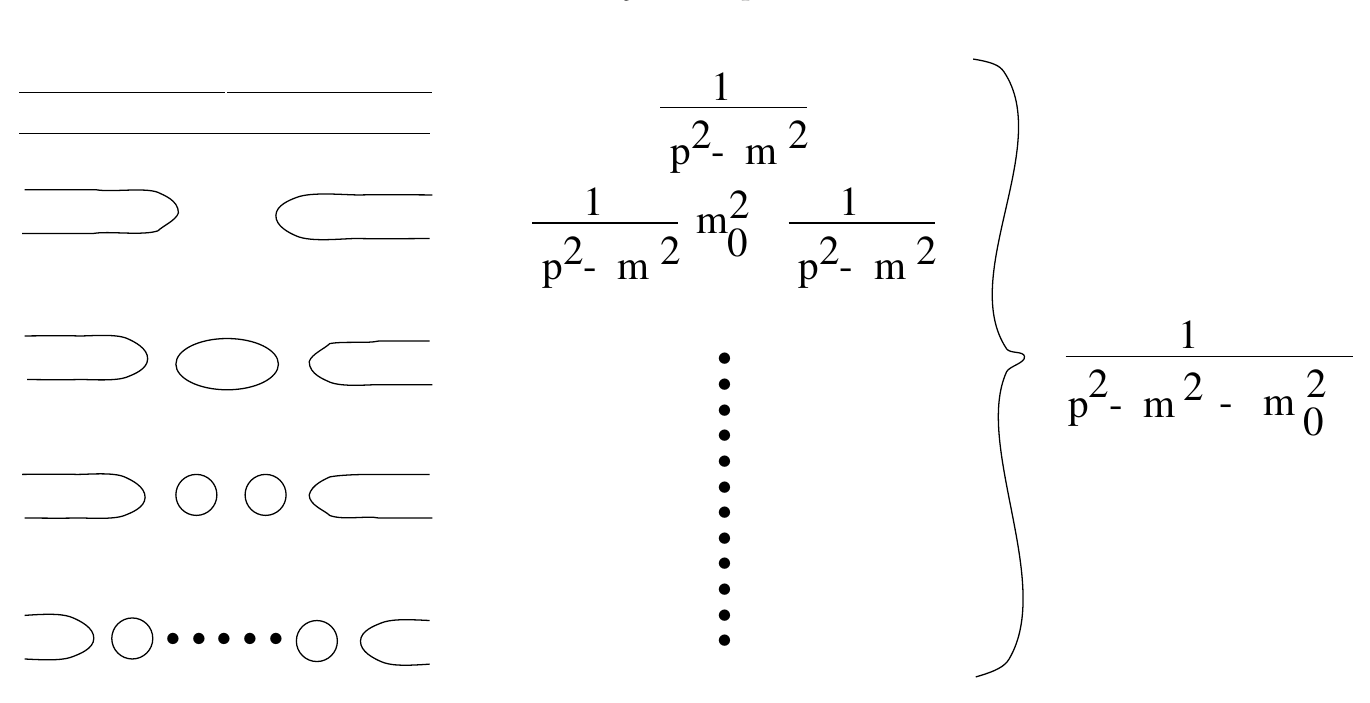
\includegraphics[width=0.8\textwidth]{images/fig18.png}
\caption{The iteration of the $\eta'$ propagator in full QCD. Only the first two diagrams survive in QQCD.}
\label{fig:18}
\end{figure}

\begin{figure}[htbp]
\centering
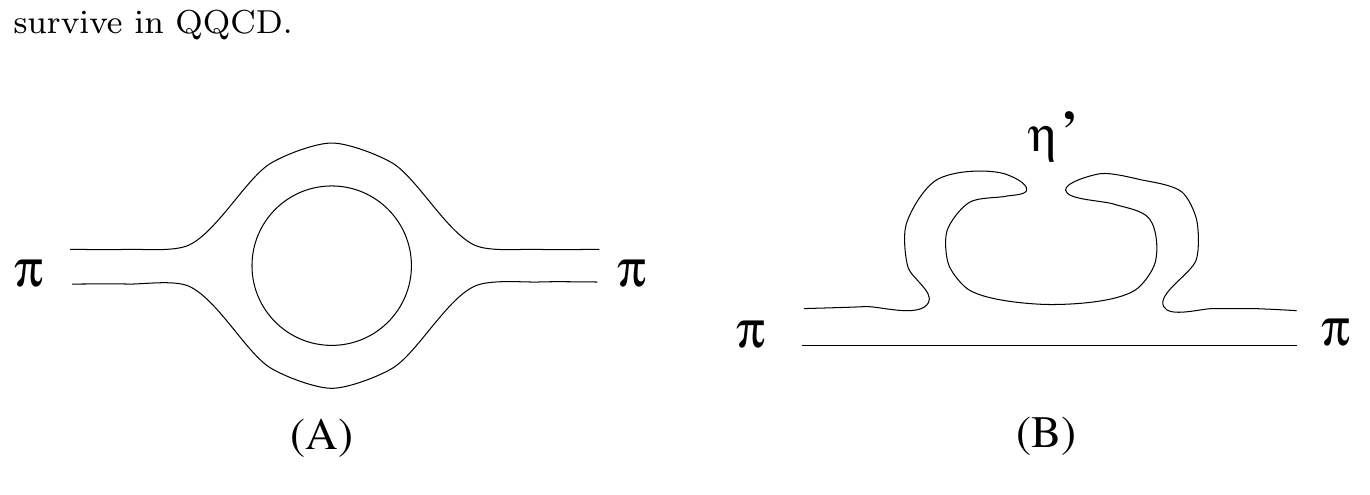
\includegraphics[width=0.8\textwidth]{images/fig19.png}
\caption{The 1-loop correction to the pion propagator in (A) full QCD (B) QQCD.}
\label{fig:19}
\end{figure}

At 1-loop full QCD has the diagram shown in Fig.~\ref{fig:19}A which is absent in QQCD. On the other hand, in QQCD, the hairpin term gives a contribution via the diagram shown in Fig.~\ref{fig:19}B. Such diagrams are neglected in full QCD as they iterate to produce a massive $\eta'$. The chiral expansions for $M_\pi$ and $f_\pi$ in full QCD have been calculated by Gasser and Leutwyler [152],
\begin{equation}
\begin{aligned}
M_\pi^2 &= 2mB\Bigl[1 + X_\pi - \frac{1}{3} X_{\eta_8} + \frac{16}{f_0^2}(2M_K^2 + M_\pi^2)(2L_6 - L_4) \\
&\qquad\qquad + \frac{16}{f_0^2} M_\pi^2 (2L_8 - L_5) + \cdots\Bigr] \\
f_\pi^2 &= f_0\Bigl[1 - 4X_\pi - 2X_K + \frac{16}{f_0^2}(2M_K^2 + M_\pi^2)L_4 + \frac{16}{f_0^2} M_\pi^2 L_5 + \cdots\Bigr]
\end{aligned}
\end{equation}
where $L_i$ are the $O(p^4)$ coefficients, $X_i = M_i^2 \log(M_i^2/\Lambda_{\chi SB}^2)/(4\pi f_0)^2$ are the chiral logs, and $f_\pi = 131$ MeV. In QQCD, Sharpe and Bernard and Golterman [150,151] find that the leading terms are
\begin{equation}
\begin{aligned}
M_\pi^{2Q} &= 2mB_Q\Bigl[1 - \delta \log\frac{M_\pi^2}{\Lambda_{\chi SB}^2} + \cdots\Bigr] \\
f_\pi^Q &= f_Q\Bigl[1 - \frac{16}{f_Q^2} M_\pi^2 \tilde{L}_5 + \cdots\Bigr]
\end{aligned}
\end{equation}
where $\delta = M_0^2 / 24\pi^2 f_\pi^2$ and $\tilde{L}_i$ are the quenched $O(p^4)$ coefficients. The term proportional to $\delta$ is a quenched chiral log and is singular in the limit $m_q = 0$.

The differences, in general, between quenched and unquenched expressions, as illustrated by the above expressions, are
\begin{itemize}
\item All the chiral constants are different in the two theories. For example, $B \neq B_Q$ and $f_0 \neq f_Q$.
\item The normal chiral logs are missing in QQCD.
\item The quenched expressions can be singular in the chiral limit due to the goldstone $\eta'$, i.e.~through terms proportional to $\delta$. These artifacts become dominant as $m_q \to 0$.
\end{itemize}

The first question raised by the analyses of Sharpe and Bernard and Golterman is---are the results of quenched $\chi$PT, an expansion about $m_q = 0$, meaningful if they are singular in that limit? We do not have a formal answer to this question. The approach adopted is to do the simulations and look for such chiral logs by doing fits with and without these terms. The status of this search has been reviewed in [153,154]. The data, while not conclusive, does suggest that $\delta \approx 0.15$, consistent with the value obtained by using phenomenological values for $M_0$ and $f_\pi$.

The second question, assuming that predictions of quenched $\chi$PT make sense, is how does one extract phenomenologically useful results for quantities that require a chiral extrapolation to $\bar{m}$? One approach is to fit the quenched data using the full QCD chiral expansions in a region of quark masses where the quenched artifacts are small. Current data suggest that this region is $m_q \gtrsim m_s/4$. In this case quenching errors are, by definition, a combination of those due to the absence of quark loops and those due to fits being made at heavier quark masses. The second possibility is to fit using the QQCD expression but extrapolate keeping only the terms in the full QCD expressions. This approach has the disadvantage of increasing the number of free parameters. In either case the hope is that there exist quantities for which the QQCD artifacts are small and the differences between QQCD and QCD coefficients are small; in such cases quenched estimates are useful phenomenological predictions. One such example is the $K^0\bar{K}^0$ mixing parameter $B_K$ [155].

In view of these various sources of systematic error, any quantity measured on the lattice depends not only on the input parameters, i.e.~the quark masses and the coupling $\alpha_s$, but also on the lattice size $L$, $a$ (discretization errors are $\propto g^m a^n$ with the powers depending on the order of improvement in the action and operators), the method used to determine the renormalization constants, and the number of dynamical quark flavors $n_f$. While the theoretical understanding of these errors is, in general, not complete, nevertheless, a lot is known and one can make consistency checks on the data. For example, the infinite volume continuum limit results for fixed $n_f$ simulations should be independent of the discretization scheme, the numerical approach used, and the definition of the renormalization constants. As of this writing, results for a number of observables show stability once extrapolated to the $L \to \infty$ and $a \to 0$ limits, albeit in the quenched approximation ($n_f = 0$). We regard this consistency check as the first important step towards providing precise results. Our optimism stems from knowing that for many phenomenologically important quantities ($B_K$, $f_D$, $f_{D_s}$, $f_B$, $f_{B_s}$, $B_B$, $\alpha_s$, and the quark masses) quenched lattice QCD results are already competitive with the best non-lattice methods, and future enhancements in methodology and computer technology will systematically improve their precision.

\chapter{Lattice Correlators}

In Section 4 we discussed the reduction of the pion 2-point correlation
function to a product of quark propagators and possibly gauge links, and its
relation to sum over states from which $M_\pi$ and $f_\pi$ can be extracted.
Here I enlarge the discussion to general 2-point and 3-point functions.
Consider the calculation of the matrix element $\langle K^+|V_\mu|D^0\rangle$
which arises in the extraction of semi-leptonic form factors.  The 3-point
correlation function needed to calculate this ME is
\begin{equation}
\begin{aligned}
C_\mu^{PVP}(t_x, p; t_y, q) &=
\sum_{x,y} e^{-i(q\cdot y+p\cdot x)}\, T[K^+ V_\mu D^0] \\
&= \sum_{x,y} e^{-i(q\cdot y+p\cdot x)}\,
   \bar{s}(0)\gamma_5 u(0)\;\bar{c}(y)\gamma_\mu s(y)\;\bar{u}(x)\gamma_5 c(x) \\
&= \sum_{x,y} e^{-i(q\cdot y+p\cdot x)}\,
   \gamma_5 S_F^u(x,0)\gamma_5 S_F^s(0,y)\gamma_\mu S_F^u(y,x) \\
&\sim \frac{\exp(-E_K(p+q)t_y - E_D(p)(t_x-t_y))}{4E_K(p+q)E_D(p)}
   \langle 0|\bar{u}\gamma_5 s|K(p+q)\rangle \\
&\qquad \times \langle K(p+q)|\bar{s}\gamma_\mu c|D(p)\rangle
   \langle D(p)|\bar{c}\gamma_5 u|0\rangle .
\end{aligned}
\end{equation}

\begin{figure}[htbp]
\centering
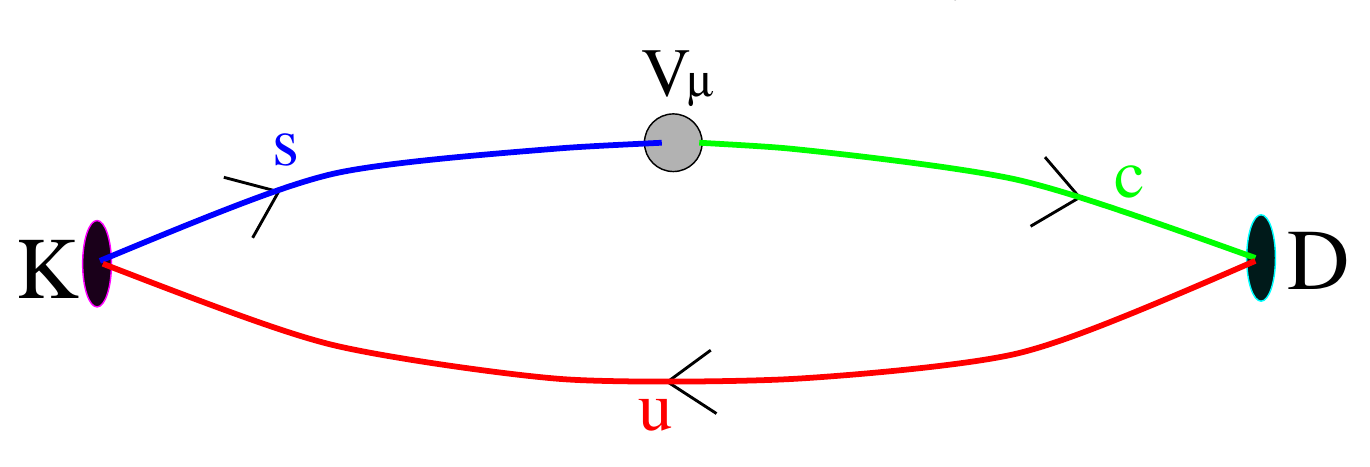
\includegraphics[width=0.8\textwidth]{images/fig20.png}
\caption{Schematic of Feynman diagram for $KV_\mu D$ in terms of $c$, $s$, and
$u$ quark propagators.}
\label{fig:20}
\end{figure}

I have used (i) Wick contractions to express the correlation function in terms
of quark propagators $S_F$ (see Fig.~20); (ii) local bilinears for the source
and sink operators and the vector current (to improve the signal one usually
uses smeared operators and an improved current); and (3) the interpolating
operator for the $D$ meson and the current insertion are at definite momentum.
Momentum conservation then fixes $p_k$.  The final form in Eq.~17.2 shows the
behavior for large Euclidean time separations ($t_x \ll t_y \ll t_0$).  Of the
many terms in the right hand side, we are only interested in the matrix element
$\langle K(p+q)|\bar{c}\gamma_\mu s|D(p)\rangle$.  The remaining factors can
all be extracted from 2-point correlation functions.  Thus, one can make
individual fits to all the required correlators, or design a ratio in which the
maximum number of unwanted factors cancel.  In practice, to improve the
numerical signal, a single fit is made to a ratio of 3-point to a combination
of 2-point functions, $T[KV_\mu D]/(T[KK]\,T[DD])$, that gets rid of the
exponential in time behavior.

To make fits to such correlation functions projected on to definite spatial
momenta, we have to address three questions:
\begin{itemize}
\item Is the correlator even or odd in its time variables?
\item Is the correlator even or odd in its momenta?
\item Is the correlator real or imaginary?  As mentioned before only the real
part of Euclidean correlation functions has a signal.
\end{itemize}

In practice we usually work in terms of bilinear operators given in Table~8
where factors of $i$ have been dropped for brevity.  In this basis of operators
one needs to know whether a given $n$-point function has a signal in the real
or imaginary part.  To answer these questions we use the discrete symmetries,
$T$, $P$, and $CPH$ discussed in Table~2 and in Eq.~10.11.  For each element of
the Dirac algebra, $\Gamma_A$ define three signs, $\tau_A$, $\pi_A$, and
$\chi_A$, associated with $T$, $P$, and $CPH$:
\begin{equation}
\begin{aligned}
\gamma_4\gamma_5\Gamma_A\gamma_5\gamma_4 &= \tau_A\Gamma_A;\\
\gamma_4\Gamma_A\gamma_4 &= \pi_A\Gamma_A;\\
C\gamma_4\gamma_5\Gamma_A\gamma_5\gamma_4 C^{-1} &= \chi_A\Gamma_A^* .
\end{aligned}
\end{equation}

\begin{table}[htbp]
\centering
\begin{tabular}{lcccccccc}
\toprule
 & $1$ & $\gamma_i$ & $\gamma_4$ & $\gamma_i\gamma_j$ & $\gamma_i\gamma_4$ & $\gamma_i\gamma_5$ & $\gamma_4\gamma_5$ & $\gamma_5$ \\
\midrule
$\tau_A$ & $+$ & $+$ & $-$ & $+$ & $-$ & $-$ & $+$ & $-$ \\
$\pi_A$ & $+$ & $-$ & $+$ & $+$ & $-$ & $+$ & $-$ & $-$ \\
$\chi_A$ & $+$ & $-$ & $+$ & $+$ & $-$ & $+$ & $-$ & $-$ \\
\bottomrule
\end{tabular}
\caption{The signs for bilinear currents under $T$, $P$ and $CPH$
transformations.}
\label{tab:7}
\end{table}

These signs are given in Table~7 and the application to 2-point and 3-point
correlators is illustrated in the next two sub-sections.

\section{Two-point meson correlators}

Consider the general two-point correlator
\begin{equation}
\begin{aligned}
C^{BA}(p,t) &= \sum_x e^{-ip\cdot x}\,
   \langle \bar{\psi}_2(x)\Gamma_B\psi_1(x)\;\bar{\psi}_1(0)\Gamma_A\psi_2(0)\rangle ,\\
&= -\sum_x e^{-ip\cdot x}\,
   \mathrm{Tr}\big(S_2(0,x)\Gamma_B S_1(x,0)\Gamma_A\big) ,
\end{aligned}
\end{equation}

where Tr is trace over spin and color indices and $t \equiv x_4$.  $T$, $P$ and
$CPH$ then imply the following:
\begin{itemize}
\item If $\tau_A\tau_B = \pm 1$, $C^{BA}(p,t)$ is even (odd) in $t$.
\item If $\pi_A\pi_B = \pm 1$, $C^{BA}(p,t)$ is even (odd) in $p$.
\item If $\chi_A\chi_B = \pm 1$, $C^{BA}(p,t)$ is real (imaginary).
\end{itemize}

Note that in Eq.~17.3 the second quark propagator is from $x \to 0$.  Using the
hermiticity property $S(x,0) = \gamma_5 S(0,x)^\dagger \gamma_5$ we can write
this in terms of $S(x,0)$.  This simple property, the relation between the
quark propagator from a given point and the anti-quark propagator to that
point, leads to a huge computational saving.  For example, if the momentum
projection is done by summing over the $L^3$ sink points $x$ with weight
$\exp(ip\cdot x)$, then, because of the hermiticity property we need only one
propagator inversion instead of $L^3+1$.

\section{Interpolating operators}

For Wilson-like fermions the interpolating field operators for mesons and
baryons at zero-momentum are given in Table~8.  The three flavors are labeled
$u$, $d$, $s$ for brevity.  The baryon operators need further clarification as
discussed in [156] and reproduced below.

\begin{table}[htbp]
\centering
\begin{tabular}{lll}
\toprule
State & $I^G(J^{PC})$ & Operator \\
\midrule
Scalar ($\sigma$) & $1^-(0^{++})$ & $u(x)d(x)$ \\
                  & $1^-(0^{++})$ & $u(x)\gamma_4 d(x)$ \\
Pseudoscalar      & $1^-(0^{-+})$ & $u(x)\gamma_5 d(x)$ \\
                  & $1^-(0^{-+})$ & $u(x)\gamma_4\gamma_5 d(x)$ \\
Vector            & $1^+(1^{--})$ & $u(x)\gamma_i d(x)$ \\
                  & $1^+(1^{--})$ & $u(x)\gamma_i\gamma_4 d(x)$ \\
Axial ($a_1$)     & $1^-(1^{++})$ & $u(x)\gamma_i\gamma_5 d(x)$ \\
Tensor ($b_1$)    & $1^+(1^{+-})$ & $u(x)\gamma_i\gamma_j d(x)$ \\
\midrule
Nucleon octet     & $(\tfrac{1}{2},\tfrac{1}{2}^-)$ & $(u_a^T C d_b)\,\gamma_5 s_c\,\epsilon_{abc}$ \\
                  & $(\tfrac{1}{2},\tfrac{1}{2}^-)$ & $(u_a^T C\gamma_5 d_b)\,s_c\,\epsilon_{abc}$ \\
Delta decuplet    & $(\tfrac{3}{2},\tfrac{3}{2}^+)$ & $(u_a^T C\gamma_i d_b)\,s_c\,\epsilon_{abc}$ \\
\bottomrule
\end{tabular}
\caption{The local interpolating field operators for mesons and baryons in
Wilson-like theories.  Projection to zero momentum states is obtained by
summing over the points $x$ on a time slice.  The $C$-parity is only relevant
for flavor degenerate meson states.  The $(\ )$ in baryon operators denote
spin trace.  $C = \gamma_2\gamma_4$ and the symmetry properties of flavor
indices for nucleons are discussed in the text.  The decuplet baryon operator
is completely symmetric in flavor index.}
\label{tab:8}
\end{table}

The spin-1/2 baryons are created by the interpolating operators
\begin{equation}
O_{(ij)k} = (\psi_{a,i}^T C\gamma_5 \psi_{b,j})\,\psi_{c,k}\,\epsilon_{abc} ,
\end{equation}

where $a$, $b$ and $c$ label color, while $i$, $j$ and $k$ label flavor.  It
is simple to show that $O_{(ij)k} = -O_{(ji)k}$, so that there are only nine
independent operators---eight $SU(3)$ octets and the singlet
$\sum_{ijk}\epsilon_{ijk}O_{ijk}$.  One way to project against the singlet is
to form
\begin{equation}
B_{ijk} = O_{(ij)k} + O_{(ik)j} = B_{ikj} .
\end{equation}

There are eight independent $B_{ijk}$'s, the relation to the usual states being
exemplified by
\begin{equation}
\begin{aligned}
\sqrt{2}\,p &= -B_{duu} = 2B_{uud} = 2B_{udu},\\
\sqrt{2}\,\Sigma^+ &= -B_{suu} = 2B_{uus} = 2B_{usu},\\
\Sigma^0 &= B_{uds} + B_{dsu} = -B_{sud},\\
\sqrt{3}\,\Lambda^0 &= B_{uds} - B_{dsu}.
\end{aligned}
\end{equation}

The overall factor in these equations is arbitrary, while the relative
normalization is fixed by $SU(3)$ symmetry.  All spin-1/2 baryon correlators
are built out of the two contractions shown in Fig.~21.  The notation
$\langle DU\rangle_S = \langle UD\rangle_S$ corresponds to quarks of flavors
$U$ and $D$ contracted into a closed loop, while the propagator for $S$ carries
the spin quantum numbers of the baryon.  The notation $(DUS)$ corresponds to a
single ordered contraction of the three quarks.  We consider two types of
correlator, ``$\Sigma$-like'' and ``$\Lambda$-like''.  The former is
exemplified by that of the $\Sigma^0$

\begin{figure}[htbp]
\centering
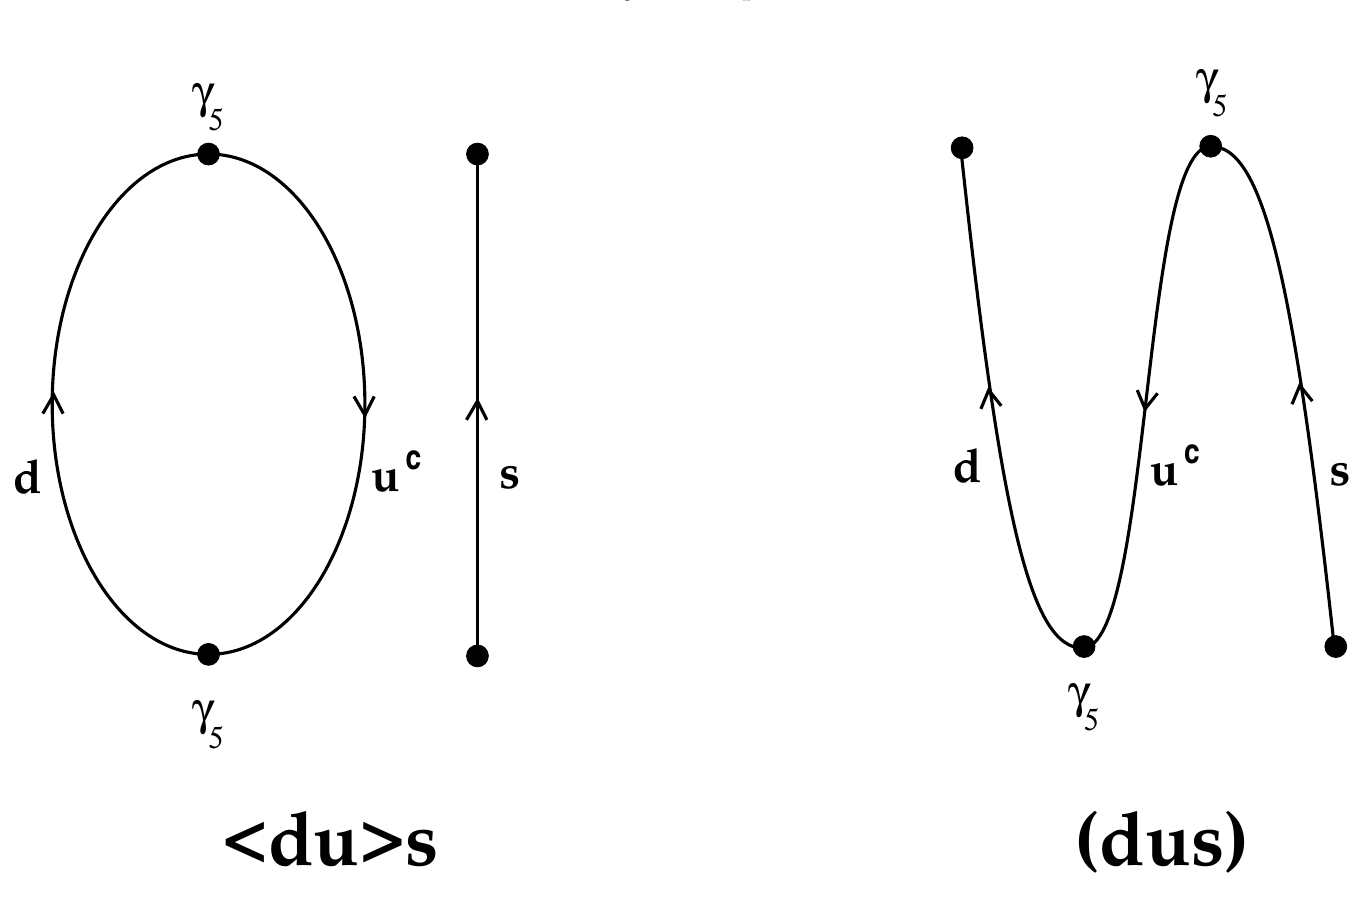
\includegraphics[width=0.8\textwidth]{images/fig21.png}
\caption{The two different types of contractions for the baryon states.}
\label{fig:21}
\end{figure}

\begin{equation}
S_{\{UD\}} = S_{\{DU\}} \equiv \langle B_{sud}(x)B_{sud}(0)\rangle
= \langle US\rangle_D + \langle DS\rangle_U + (USD) + (DSU) .
\end{equation}

This equation defines the sign conventions for the contractions.  The proton,
neutron, $\Sigma^+$, $\Sigma^-$, $\Xi^0$ and $\Xi^-$ correlators are also of
this type: they are, respectively, $D\{UU\}$, $U\{DD\}$, $S\{UU\}$, $S\{DD\}$,
$U\{SS\}$ and $D\{SS\}$.  The second type of correlator is that of the
$\Lambda^0$
\begin{equation}
\begin{split}
S_{[UD]} = S_{[DU]} &\equiv \tfrac{1}{3}\Big[\langle US\rangle_D + \langle DS\rangle_U + 4\langle UD\rangle_S\\
&\qquad - (USD) - (DSU) + 2(SUD) + 2(SDU) + 2(UDS) + 2(DUS)\Big] .
\end{split}
\end{equation}

When $m_u \neq m_d$, there is also a non-vanishing $\Lambda^0 - \Sigma^0$ cross
correlator, for which no useful results have been found [156].
Correlators of the form $A[AB]$ and $A\{AB\}$ are not independent---they are
related by
\begin{equation}
\begin{aligned}
A_{[AB]} &= \tfrac{1}{4}(3B_{[AA]} + B_{\{AA\}}),\\
A_{\{AB\}} &= \tfrac{1}{4}(B_{[AA]} + 3B_{\{AA\}}) .
\end{aligned}
\end{equation}

One can think of the results for the $A\{BB\}$ and $A[BB]$ masses as being
those for the $\Sigma$ and $\Lambda$, respectively, with $m_s = m_A$ and
$m_u = m_d = m_B$.  Unlike in the real world, there is nothing to stop
$m_A = m_B$.  Note, however, that in this case the $\Sigma$ and $\Lambda$ are
also degenerate, i.e.\ $M(A\{AA\}) = M(A[AA])$.  Indeed, the contractions in
the two cases are identical.

The interpretation of the results for the completely non-degenerate
correlators, $A[BC]$ and $A\{BC\}$, is more complicated.  Because isospin is
broken, the $\Sigma^0$- and $\Lambda$-like states mix, with both correlators
containing contributions from both physical states.  Let $M_+$ and $M_-$ be the
masses of the heavier and lighter states, respectively, and $\delta M$ the mass
difference.  At long times, the effective mass for both correlators will
asymptote to $M_-$.  However, at times short compared to the inverse mass
difference, i.e.\ $\delta M\,t_{\max} \ll 1$, there will be an approximate
plateau at a value which is a weighted average of the two masses.  The
surprising result, derived at lowest order in the chiral expansion in [156],
is that the masses extracted from these short time plateau are insensitive to
the isospin breaking and can be interpreted as those for $A[DD]$ and $A\{DD\}$
where $D = (B+C)/2$ is the mean mass for the two quarks.

\section{Three-point correlators}

A general three-point correlation function of meson operators and bilinear
currents has the form
\begin{equation}
\begin{aligned}
C^{CBA}(q,t_y;p,t_x) &= \sum_{x,y} e^{-i(q\cdot y+p\cdot x)}\,
   \langle \bar{\psi}_3(y)\Gamma_C\psi_2(y)\;\bar{\psi}_2(x)\Gamma_B\psi_1(x)
   \;\bar{\psi}_1(0)\Gamma_A\psi_3(0)\rangle ,\\
&= -\sum_{x,y} e^{-i(q\cdot y+p\cdot x)}\,
   \mathrm{Tr}\big(S_3(0,y)\Gamma_C S_2(y,x)\Gamma_B S_1(x,0)\Gamma_A\big) ,
\end{aligned}
\end{equation}

where $t_x \equiv x_4$ and $t_y \equiv y_4$.  $T$, $P$ and $CPH$ imply
\begin{itemize}
\item If $\tau_A\tau_B\tau_C = \pm 1$, $C^{CBA}(q,t_y;p,t_x)$ is even (odd)
under the simultaneous inversion of $t_x$ and $t_y$.
\item If $\pi_A\pi_B\pi_C = \pm 1$, $C^{CBA}(q,t_y;p,t_x)$ is even (odd) under
the simultaneous inversion of $p$ and $q$.
\item If $\chi_A\chi_B\chi_C = \pm 1$, $C^{CBA}(q,t_y;p,t_x)$ is real
(imaginary).
\end{itemize}

\section{CPS Symmetry}

The theory has an additional discrete symmetry, $CPS$, where $S$ is the
symmetry between switching $s$ and $d$ quarks [157].  This symmetry holds both
on the lattice and in the continuum for $m_d = m_s$.  For $m_d \neq m_s$ the
symmetry is softly broken, i.e., violations are proportional to $m_s - m_d$.
This symmetry plays a very useful role in the calculation of weak matrix
elements for it (i) restricts the set of possible Wick contractions, and (ii)
restricts the set of operators that mix with each other.

For a simple illustration consider $(\bar{s}\gamma_\mu Lu)(\bar{u}\gamma_\mu
Ld)$, a local 4-quark operator which is even under $CPS$
\begin{equation}
\begin{aligned}
(\bar{s}\gamma_\mu Lu)(\bar{u}\gamma_\mu Ld)
&\xrightarrow{P} (\bar{s}\gamma_4\gamma_\mu L\gamma_4 u)(\bar{u}\gamma_4\gamma_\mu L\gamma_4 d)\\
&\xrightarrow{C} (s^T C^{-1}\gamma_4\gamma_\mu L\gamma_4 C\bar{u}^T)(u^T C^{-1}\gamma_4\gamma_\mu L\gamma_4 C\bar{d}^T)\\
&= (s^T\gamma_4\gamma_\mu^T L\gamma_4\bar{u}^T)(u^T\gamma_4\gamma_\mu^T L\gamma_4\bar{d}^T)\\
&= (s^T\gamma_\mu^T R\bar{u}^T)(u^T\gamma_\mu^T R\bar{d}^T)\\
&= (\bar{u}R\gamma_\mu s)(\bar{d}R\gamma_\mu u)\\
&= (\bar{u}\gamma_\mu Ls)(\bar{d}\gamma_\mu Lu)\\
&\xrightarrow{S} (\bar{u}\gamma_\mu Ld)(\bar{s}\gamma_\mu Lu)
\end{aligned}
\end{equation}

The brackets denote trace over spin and color and the final reordering of the
two traced terms is allowed as time-ordering is implicit when calculating
expectation values.

This symmetry has a further generalization as discussed by Bernard and Soni in
[2,6].  For 4-fermion operators of the form $(\bar{\psi}_1\Gamma_A\psi_2)
(\bar{\psi}_3\Gamma_B\psi_4)$, there are two general switchings: (i)
$CPS'$ corresponding to $1 \leftrightarrow 2$ and $3 \leftrightarrow 4$, and
(ii) $CPS''$ corresponding to $1 \leftrightarrow 4$ and $2 \leftrightarrow 3$.
Bernard and Soni show in [2,6] how these switching symmetries are used to
restrict (i) the possible contractions in the decay $K \to \pi\pi$ via the
operator $(\bar{s}\gamma_\mu Lu)(\bar{u}\gamma_\mu Ld)$, and (ii) the mixing of
$O_\pm \equiv (\bar{s}\gamma_\mu Ld)(\bar{u}\gamma_\mu Lu) \pm
(\bar{s}\gamma_\mu Lu)(\bar{u}\gamma_\mu Ld) - (u \to c)$ with other operators.
I leave the details of these calculations as an exercise for the reader.

% SECTION 18: Lattice Calculations of the Hadron Spectrum
% R. Gupta, "Introduction to Lattice QCD" (arXiv:hep-lat/9807028)

\chapter{Lattice Calculations of the Hadron Spectrum}

Successful calculations of the spectrum will test QCD. The basic steps in the lattice analysis are discussed in Sections~4 and~17. For a given set of input parameters, the mass of a given state is determined from the rate of exponential fall-off of the connected 2-point correlation function
\begin{equation}
\Gamma(\tau) \equiv \langle O_f(\tau) O_i(0) \rangle - \langle O_f \rangle \langle O_i \rangle
= \sum_n \frac{\langle 0 | O_f | n \rangle \langle n | O_i | 0 \rangle}{2 M_n}\, e^{-M_n \tau}.
\label{eq:2pt}
\end{equation}

We shall assume that the sum over $n$ is restricted to the desired state by (i) optimizing $O_i$ and $O_f$ to get a large overlap with the wave function, i.e.\ make desired state $\langle n | O | 0 \rangle$ large and the rest small, (ii) increasing the statistics so that the signal extends to large enough $\tau$ at which any remaining contamination from higher states is negligible; and (3) making a zero-momentum projection on either $O_i$ or $O_f$. I shall further assume that the spectrum of possible states is discrete and has a mass-gap. Then, in order to extract $M$ it is useful to define an effective mass
\begin{equation}
M_{eff}(\tau) = \log\!\left( \frac{\Gamma(\tau-1)}{\Gamma(\tau)} \right)
\label{eq:meff}
\end{equation}
which, in the limit $\tau \to \infty$, converges to the desired value. The anatomy of the behavior of $M_{eff}(\tau)$ for two different states (pion and nucleon) and for two different choices of $O_i$ and $O_f$ are shown in Figs.~\ref{fig:22} and~\ref{fig:23}. The points to note are:
\begin{itemize}
\item The convergence to the asymptotic value $M$ can be from above or below depending on the choice of $O$. Only for $O_f = O_i^\dagger$ is the correlation function positive definite and the convergence is monotonic and from above.
\item For $O_f \neq O_i^\dagger$, the convergence depends on subtle cancellations between contributions of various states. The relative signs are given by the product of the two amplitudes $\langle n | O_f | 0 \rangle \langle n | O_i | 0 \rangle$. Since this sign for state $|n\rangle$ can be plus or minus, the convergence is neither guaranteed to be monotonic nor from above.
\end{itemize}

\begin{figure}[htbp]
\centering
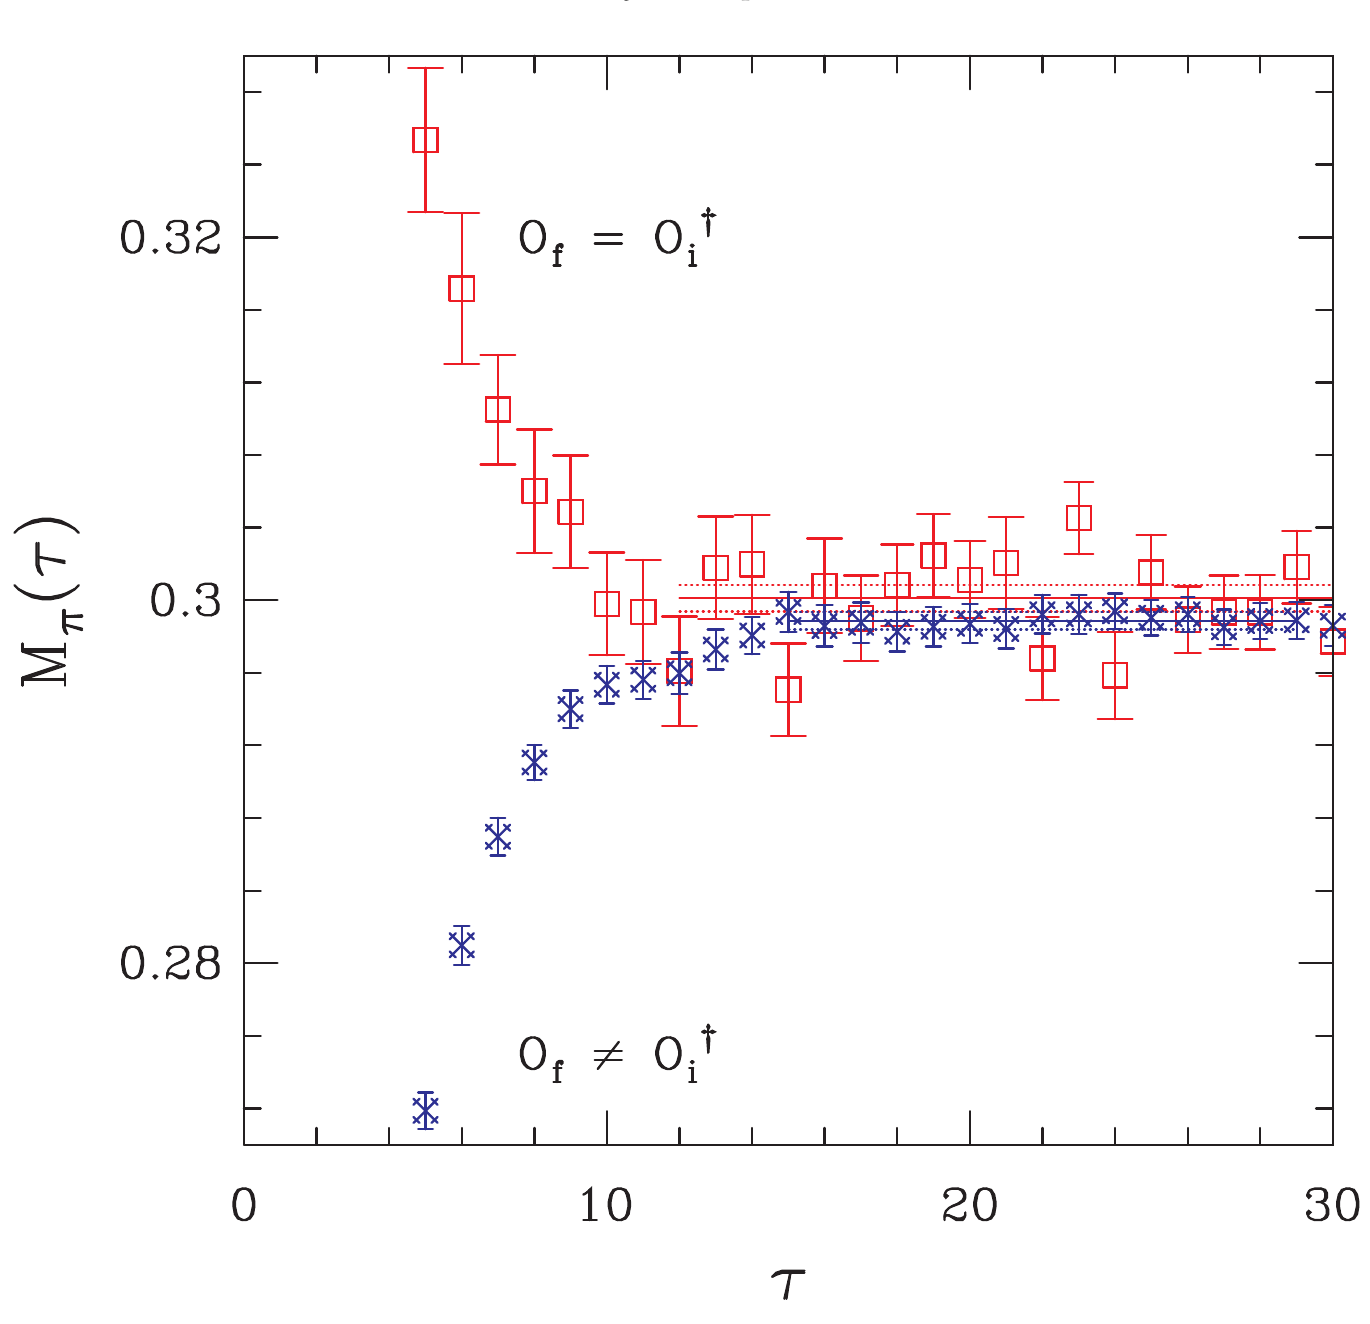
\includegraphics[width=0.8\textwidth]{images/fig22.png}
\caption{Effective mass plots for $M_\pi$ versus $\tau$. The horizontal lines denote the estimate of the asymptotic value of $M$ and the range of the plateau used in the fits, while the dotted lines show the error. The squares denote data for smeared-smeared interpolating operators ($O_f = O_i^\dagger$), while fancy crosses show data with wall-local operators.}
\label{fig:22}
\end{figure}

\begin{itemize}
\item The contribution of excited states is most obvious at small $\tau$, where $M_{eff}$ varies rapidly before flattening out. For $\tau$ in this flat (called plateau) region one assumes that, within the numerical precision, only the lowest state contribution is significant.
\item The location in $\tau$ of the onset and the length of the plateau region depends on the interpolating operators.
\item For a finite statistical sample the plateau region is not flat but the data usually exhibit correlated fluctuations [158]. Therefore, unless the plateau is long enough that the fit can average over a few cycles, the extracted $M_{eff}$ can be biased by these statistical fluctuations.
\end{itemize}

\begin{figure}[htbp]
\centering
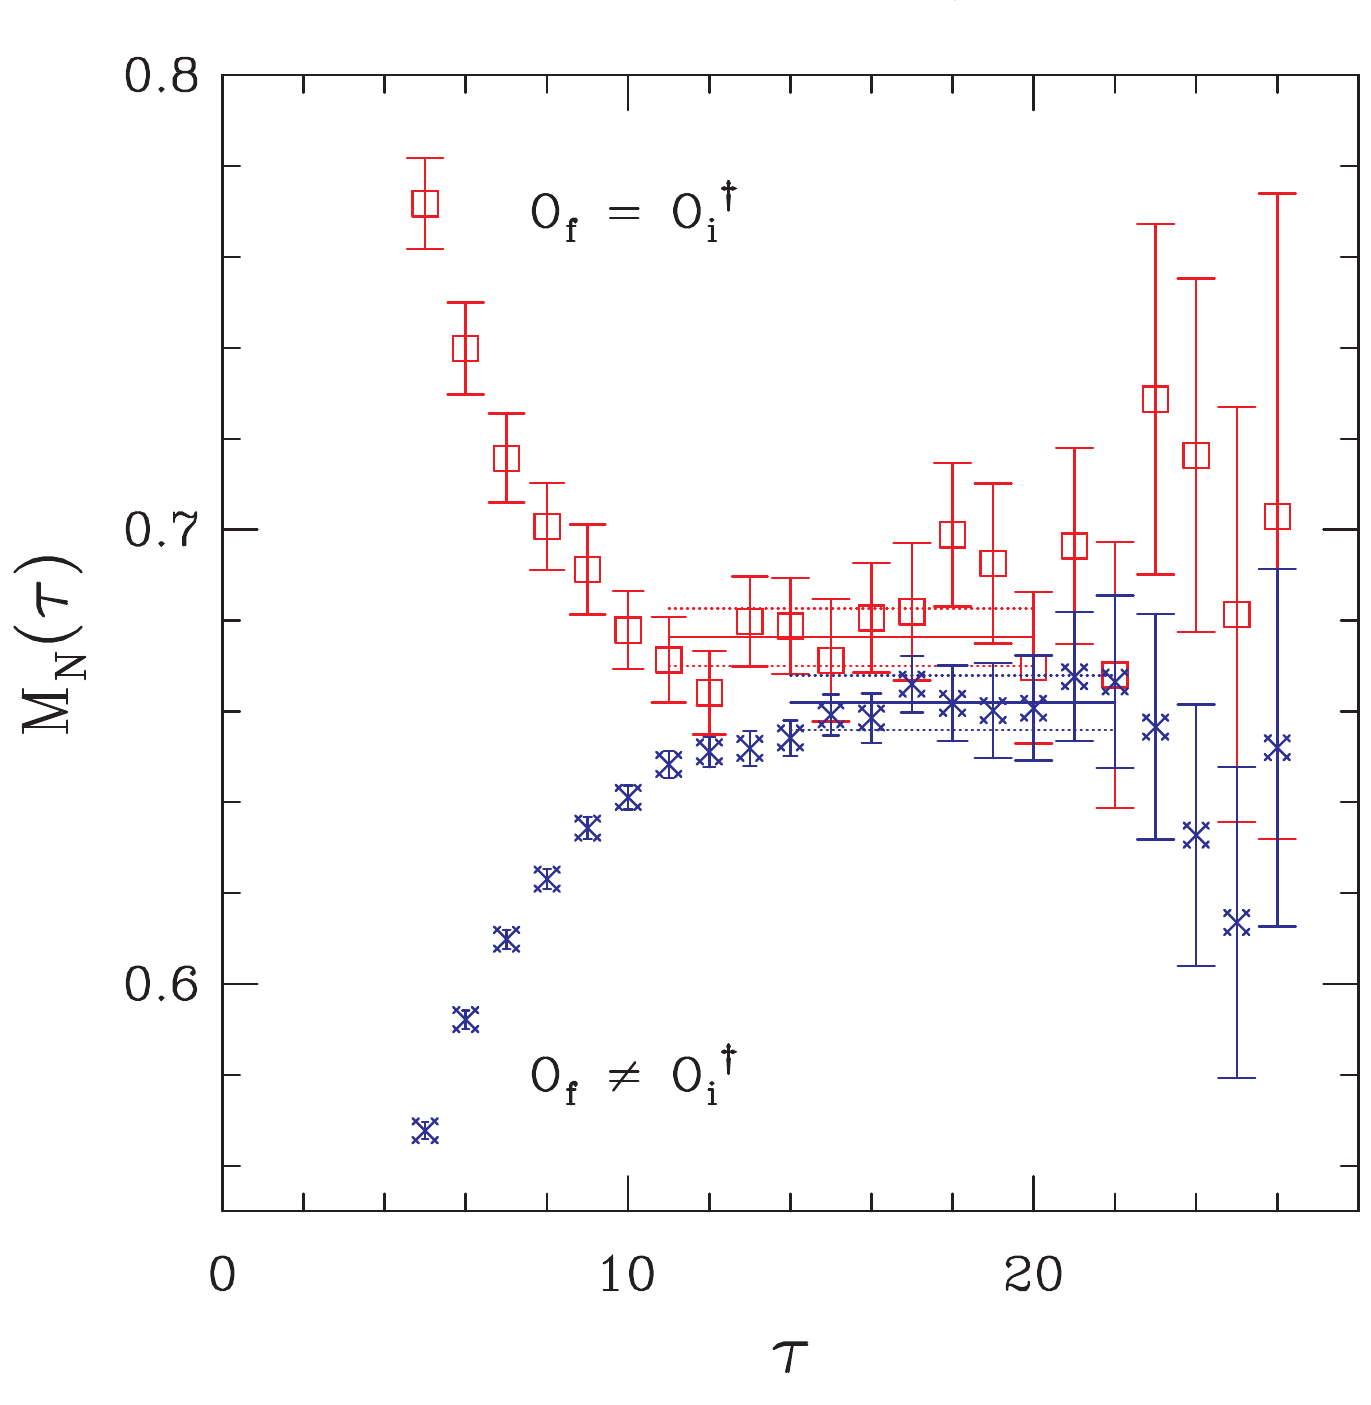
\includegraphics[width=0.8\textwidth]{images/fig23.png}
\caption{Effective mass plots for $M_N$ versus $\tau$. The rest is the same as in Fig.~\ref{fig:22}.}
\label{fig:23}
\end{figure}

\begin{itemize}
\item The statistical errors grow with $\tau$, except for the case of the pion. The reason for this was elucidated by Lepage in [159] and a synopsis of his argument is as follows. For a state with $N$ valence quark lines, where $N = 2(3)$ for mesons (baryons), the errors are controlled by the square of the correlator which has $2N$ lines. The state of lowest energy in the squared correlator is, therefore, two pions for mesons and three pions for baryons. Thus, while the signal decreases as $\exp(-M \tau)$, the noise only decreases as $\exp(-M_\pi \tau \times N/2)$. Consequently, all states for which $M > N M_\pi / 2$ the errors will increase with $\tau$. The only exception to this condition is the pion for which the signal and noise have the same $\tau$ dependence.
\item In cases where there is no clear plateau (the signal does not extend far enough in $\tau$), one can make a fit to a larger range of $\tau$ by including the contribution of higher (radial) states in the sum in Eq.~\eqref{eq:2pt}. This is illustrated in Fig.~\ref{fig:24} for a two state fit which involves four free parameters, two amplitudes and two masses. The amplitude and mass of the excited state are less well constrained as they are trying to mimic the effect of a number of states, consequently such fits may show significant dependence on the range of $\tau$ selected. One can refine the excited state parameters by iteratively improving single state fits to $\Gamma(\tau) - \Gamma_0(\tau)$ at short $\tau$ and to the ground state $\Gamma_0(\tau)$ at large $\tau$ until the whole range is covered. A better approach to gain confidence in ground state parameters is to make simultaneous fits to a matrix of correlation functions created with different source and sink operators with the same quantum numbers. For a matrix with $m$ ($n$) distinct sources (sinks) the simultaneous fit is more constraining as it involves $m + n$ amplitudes but a single common mass.
\end{itemize}

\begin{figure}[htbp]
\centering
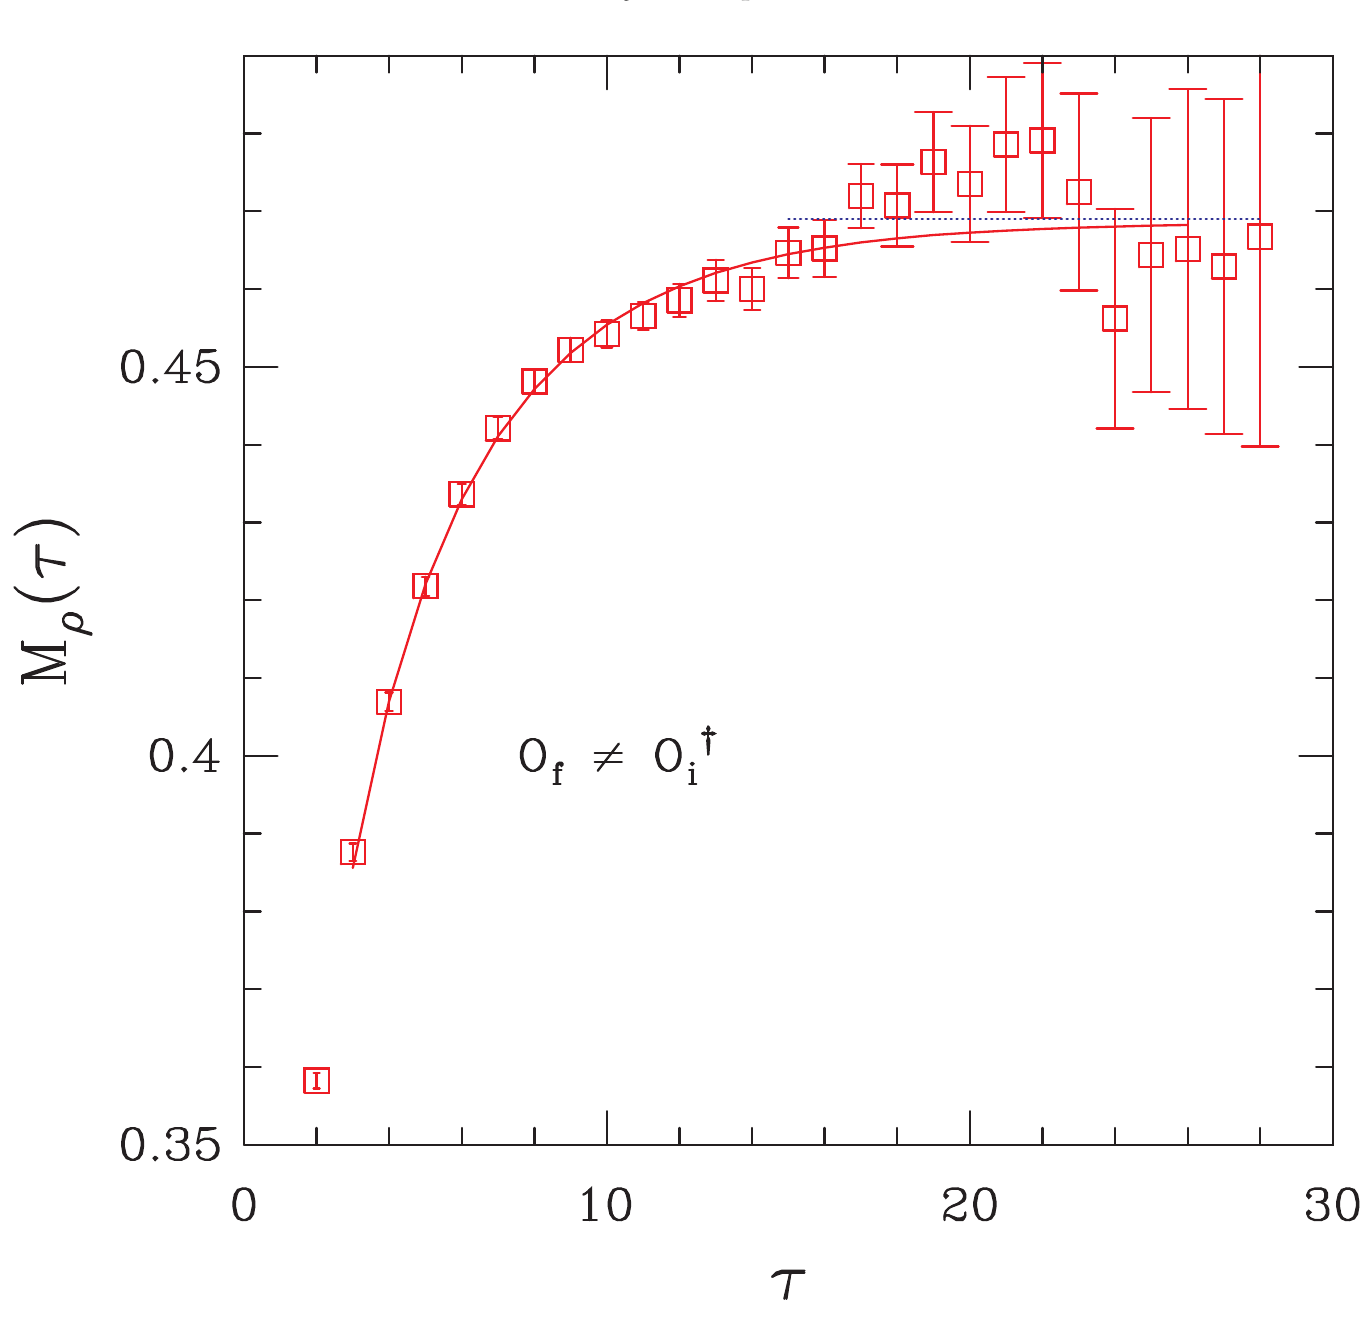
\includegraphics[width=0.8\textwidth]{images/fig24.png}
\caption{Effective mass plots for $M_\rho$ versus $\tau$ for the wall-local source. Since there is no clear plateau, a fit including two states is made to $3 \leq \tau \leq 26$. From such fits the masses of $\rho$ and $\rho^*$ are obtained. The mass of the $\rho$ from the 2-state fit is consistent with that from a single state fit to data at $\tau > 15$ (blue dotted line).}
\label{fig:24}
\end{figure}

To summarize, we mostly extract $M$ from fits to an intermediate range of $\tau$, the ``plateau'' region, where $M_{eff}$ is essentially independent of $\tau$. At small $\tau$ the influence of excited states is large, while at large $\tau$ the statistical noise overwhelms the signal. Accuracy of the result depends on the presence of a plateau extending over a large range of $\tau$ that averages a few cycles of correlated fluctuations. The data in Figs.~\ref{fig:22}, \ref{fig:23}, and \ref{fig:24} show that, with 170 lattices of size $32^3 \times 64$ at $1/a = 2.3$ GeV, this is true for the pion but marginal for other states like the vector mesons and baryons. Our present estimate is that roughly 1000 independent lattices are necessary to get a reliable signal that leads to 0.1--0.4\% accuracy in baryon masses with quark masses in the range $m_s - m_s/4$ respectively.

Assuming that the above steps have been carried out and we have reliable estimates for hadron masses as a function of quark masses, $a$, $L$, and the number $n_f$ of dynamical flavors, we are finally in a position to compare them to experimental data.

\section{Status of the Light Meson and Baryon Spectrum}

The first test of QCD is to reproduce the masses of pseudoscalar mesons (PS = $\{\pi, K, \eta\}$), vector mesons (V = $\{\rho, K^*, \omega, \phi\}$), octet baryons ($B_8 = \{N, \Sigma, \Xi, \Lambda\}$), and decuplet baryons ($B_{10} = \{\Delta, \Sigma^*, \Xi^*, \Omega\}$) from simulations with four input parameters $m_u$, $m_d$, $m_s$, and $\alpha_s$. I will assume that the lattices are large enough that finite size effects can be neglected. The remaining important issues are
\begin{itemize}
\item Simulations have mainly been done in the quenched approximation. Rather than testing QCD, these calculations quantify the accuracy of QQCD.
\item Isospin breaking effects and electromagnetic contributions are neglected.
\item Simulations have been done with unphysical values of quark masses, typically in the range $[2m_s - m_s/4]$. To get physical results the data are extrapolated to $m = (m_u + m_d)/2$ using functional forms predicted by (quenched) chiral perturbation theory.
\end{itemize}

The first step in the analyses is to extrapolate the data to physical values of $m$ and $m_s$. The simplest Ans\"atze are the lowest order chiral expressions
\begin{equation}
\begin{aligned}
M_{PS}^2 a^2 &= B_{PS} a^2 (m_1 + m_2)/2 + \cdots, \\
M_V a &= A_V + B_V a (m_1 + m_2)/2 + \cdots, \\
M_\Sigma a &= A_N + 4F m a + 2(F - D) m_s a + \cdots, \\
M_\Lambda a &= A_N + 4(F - D/3) m a + 2(F + D/3) m_s a + \cdots, \\
M_{10} a &= A_{10} + B_{10} a (m_1 + m_2 + m_3)/3 + \cdots.
\end{aligned}
\label{eq:chiral}
\end{equation}

From these fits we determine the constants $A_V$, $A_N$, $A_{10}$ and $B_{PS}$, $B_V$, $F$, $D$, $B_{10}$. Then using a suitable set, for example $A_V$, $B_{PS}$, $B_V$ or $A_{10}$, $B_{PS}$, $B_{10}$, we fix the three input parameters $1/a$, $m$, $m_s$. Unless otherwise stated the following discussion will assume that $m$, $a$, and $m_s$ have been fixed using $M_\pi$, $M_\rho$, and $M_\phi$ (or equivalently $M_{K^*}$) respectively. The question then is --- how well do the masses of the remaining states compare with experimental numbers?

This simple analysis to test QCD (or to quantify the quenched approximation) can fall short in two ways. First, the data could show significant deviations from the linear relations Eq.~\eqref{eq:chiral}. In that case the analysis becomes much more elaborate due to the increase in the number of free parameters; the possible leading non-linear terms include $O(m^2)$ corrections and chiral logarithms. To disentangle these requires very precise data at a number of values of $m_q$ in the range $m_s/4 - 3m_s$, however, such a possibility of physics richer than that predicted by the ``naive'' quark model is exciting. The second possible failing is that different sets of states used to fix $a$, $m$, $m_s$ give different results. There could be three reasons for this failure: (i) The coefficients extracted from simulations at the significantly heavier values of $m_q$ change as the quark masses are decreased; (ii) the differences are artifacts of discretization errors and vanish in the limit $a = 0$; (3) quenching errors. The current data show evidence for non-linearities in fits in $m_q$ [156,160]. Also, the $a$, $m$, $m_s$ extracted from different sets are significantly different, and all three causes listed above contribute. As a result the focus of current analyses has been to first disentangle and quantify the contributions of the various artifacts. I will briefly illustrate these effects.

Let me start with evidence for non-linear terms in the chiral fits. Fig.~\ref{fig:25} is an example of the behavior of the vector meson mass as a function of the quark mass [156]. The plot makes it clear that in order to quantify the deviations one needs very precise data over a large range of $m_q$. With a statistical accuracy of $\sim 0.5\%$, a linear fit works for $0.02 \leq ma \leq 0.04$ corresponding to $50 \leq m \leq 100$ MeV, but not for the full range. The leading chiral corrections are proportional to $m^{3/2}$ from chiral loops, and $m^2$. Including either term allows fits over the full range, and the data are not precise enough to distinguish between them. The effect of these non-linearities seems to be small, for example the change in $M_\rho$, after extrapolation to $m$, is $\sim < 1\%$ on including either of the higher order terms in the fit.

\begin{figure}[htbp]
\centering
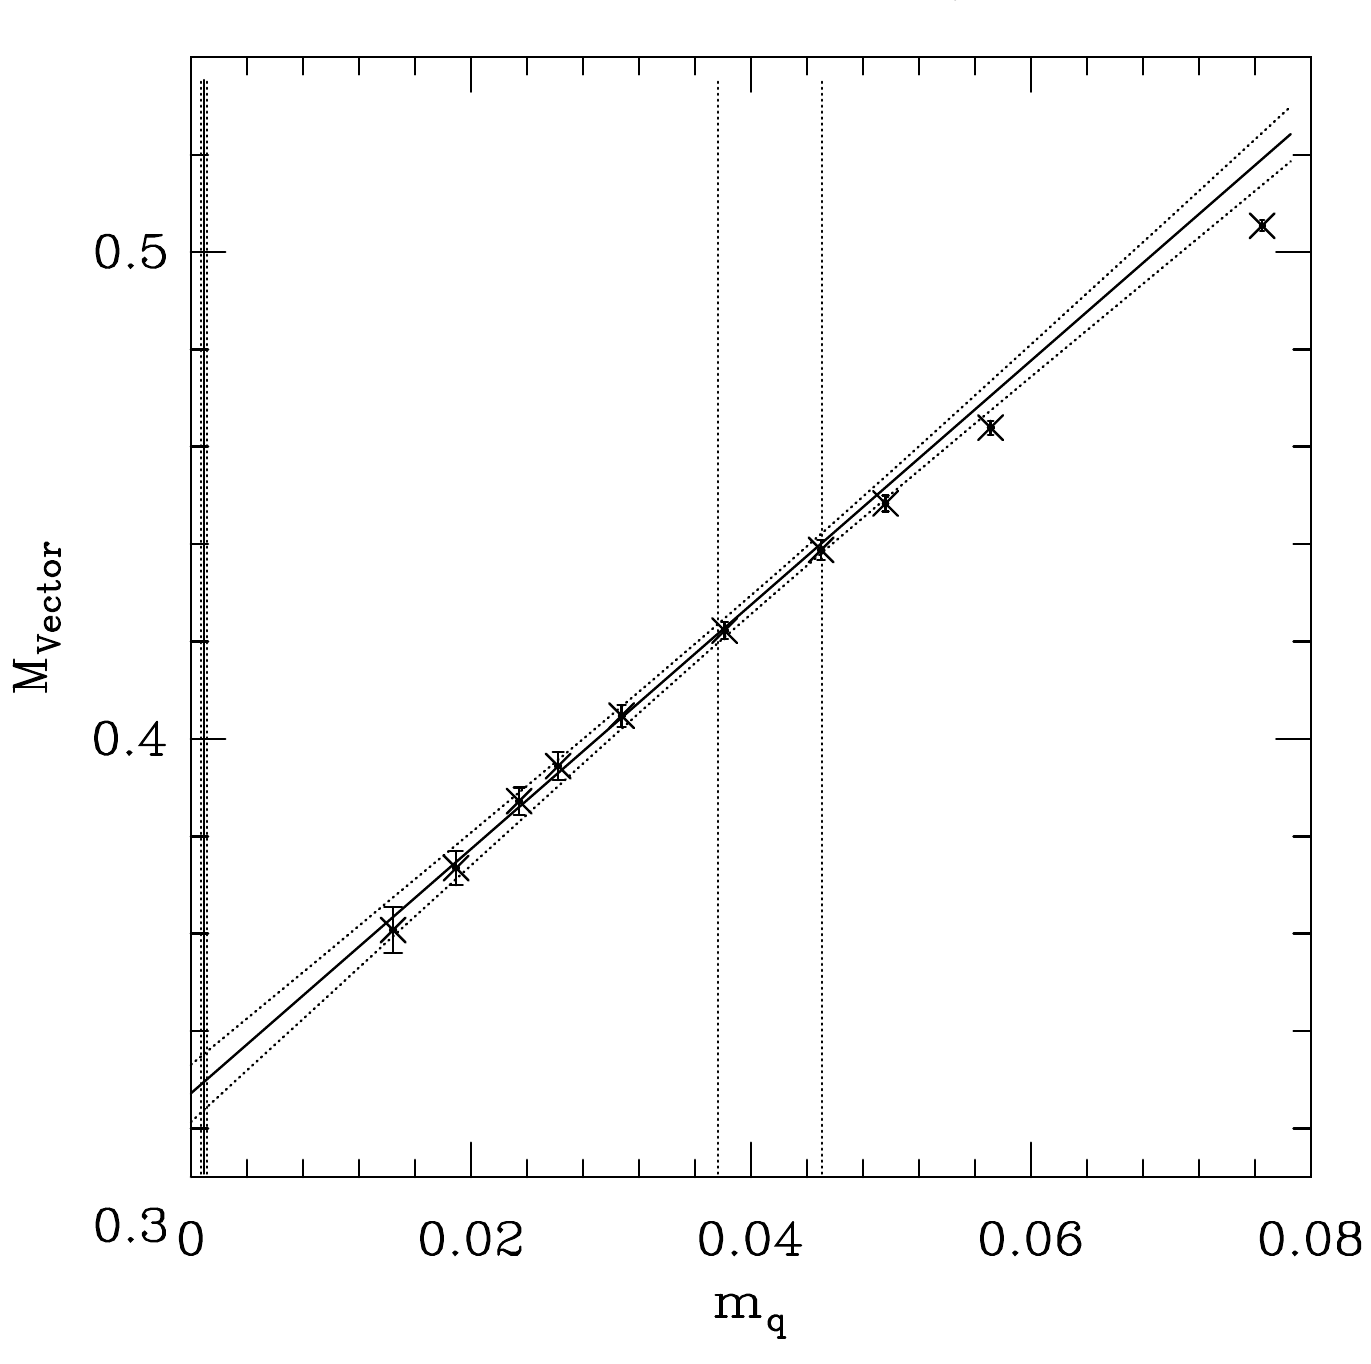
\includegraphics[width=0.8\textwidth]{images/fig25.png}
\caption{Plot of $M_{vector}$ versus the quark mass $m$. The data, reproduced from [156], were obtained on $32^3 \times 64$ quenched lattices at $\beta \equiv 6/g^2 = 6$ corresponding to $1/a = 2.33(4)$ GeV. The linear fit is to the lightest six points. The vertical lines show $m$ and the range of estimates of $m_s$.}
\label{fig:25}
\end{figure}

The first test of the quenched approximation is whether it can reproduce the hyperfine splittings in the meson sector. Figure~\ref{fig:26} shows some current data. The only input quantity is the scale $1/a$ which is used to convert lattice masses to physical units. If $M_\pi$ and $M_\rho$ are used to set $m$ and $1/a$ respectively, then the curves, by construction, have to pass through the experimental point at $M_{PS} = M_\pi$. Different choices for the scale setting quantity will change $1/a$ and shift the curves as a whole.

\begin{figure}[htbp]
\centering
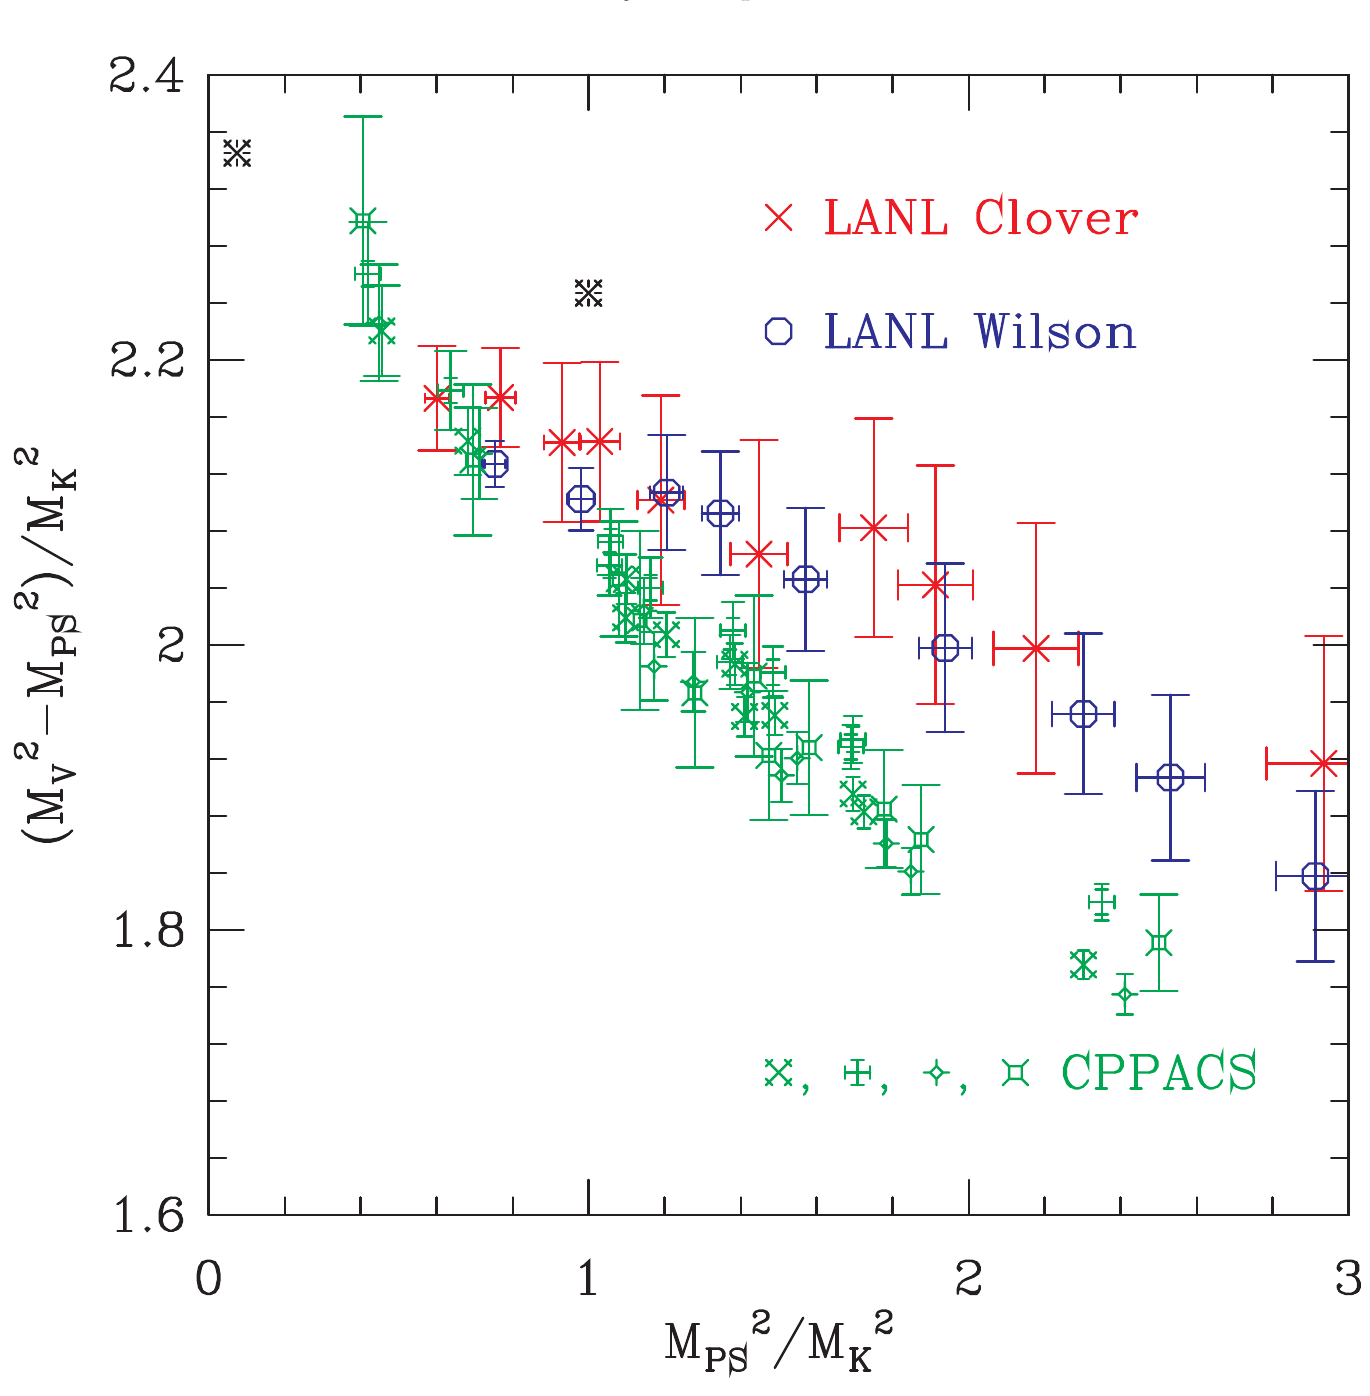
\includegraphics[width=0.8\textwidth]{images/fig26.png}
\caption{Hyperfine splittings in the meson sector. Quenched data from (i) LANL collaboration with Wilson fermions (blue octagons) [156], (ii) LANL collaboration with tadpole improved clover fermions (red crosses) [162], and (iii) CP-PACS collaboration Wilson runs at $\beta = 5.9, 6.1, 6.25, 6.47$ (green fancy crosses, pluses, diamonds, and squares) [161]. The experimental points are shown by the symbol burst.}
\label{fig:26}
\end{figure}

On the other hand, the slope at any given point is independent of the lattice scale, and is therefore the more robust lattice prediction. For this reason the quantity $J \equiv M_V \, \partial M_V / \partial M_{PS}^2$ is commonly used as a test of the hyperfine splittings. Lattice data (for a review see [161]) gives values for $J$ that are $\sim 20\%$ too small. Another manifestation of this discrepancy will appear in Section~20 where I show that the estimates of $m_s$ fixed using $M_K$ versus $M_{K^*}$ (or $M_\phi$) differ by $\sim 15\%$.

The data shown in Fig.~\ref{fig:26} allow two comparisons. First, the octagons (blue points) and crosses (red) are LANL data from the same 170 quenched $32^3 \times 64$ lattices at $\beta = 6.0$ with the Wilson and tadpole improved clover Dirac actions [156,162]. One does not find any significant improvement with clover fermions. Second, the fancy crosses, pluses, diamonds, and squares (green points) are Wilson fermion data from CP-PACS collaboration at $\beta = 5.9, 6.1, 6.25, 6.47$ [161]. The data at the four $\beta$ values are consistent. Both comparisons imply that the smaller splittings are not due to discretization errors.

The data in Fig.~\ref{fig:26} also show a difference between the CP-PACS and LANL Wilson fermion results at quark masses heavier than $m_s$. This is surprising since in this regime both collaborations have reliable measurements of the vector and pseudoscalar masses. The culprit is the lattice scale. It turns out that the estimate of $1/a$ from LANL data is 3\% larger compared to the value obtained by an interpolation of the CP-PACS data. Adjusting the LANL scale shifts their data as a whole and makes all the results overlap.

The conclusion, from this and other quenched data, is that the splittings come out too small. Even though the size of discretization errors is, in my opinion, not fully resolved, the deviations are thought to be mostly due to the use of the quenched approximation.

The most extensive discussion of the mass-splittings in the baryon octet and decuplet using the Wilson action is given in [156]. Note that since this calculation was done at only one $1/a \approx 2.3$ GeV, therefore discretization errors are not resolved. There are two important observations. (i) The mass splittings in the baryon octet show significant non-linearities, for example the dependence of $M_\Sigma - M_\Lambda$ on the quark mass is shown in Fig.~\ref{fig:27}.

\begin{figure}[htbp]
\centering
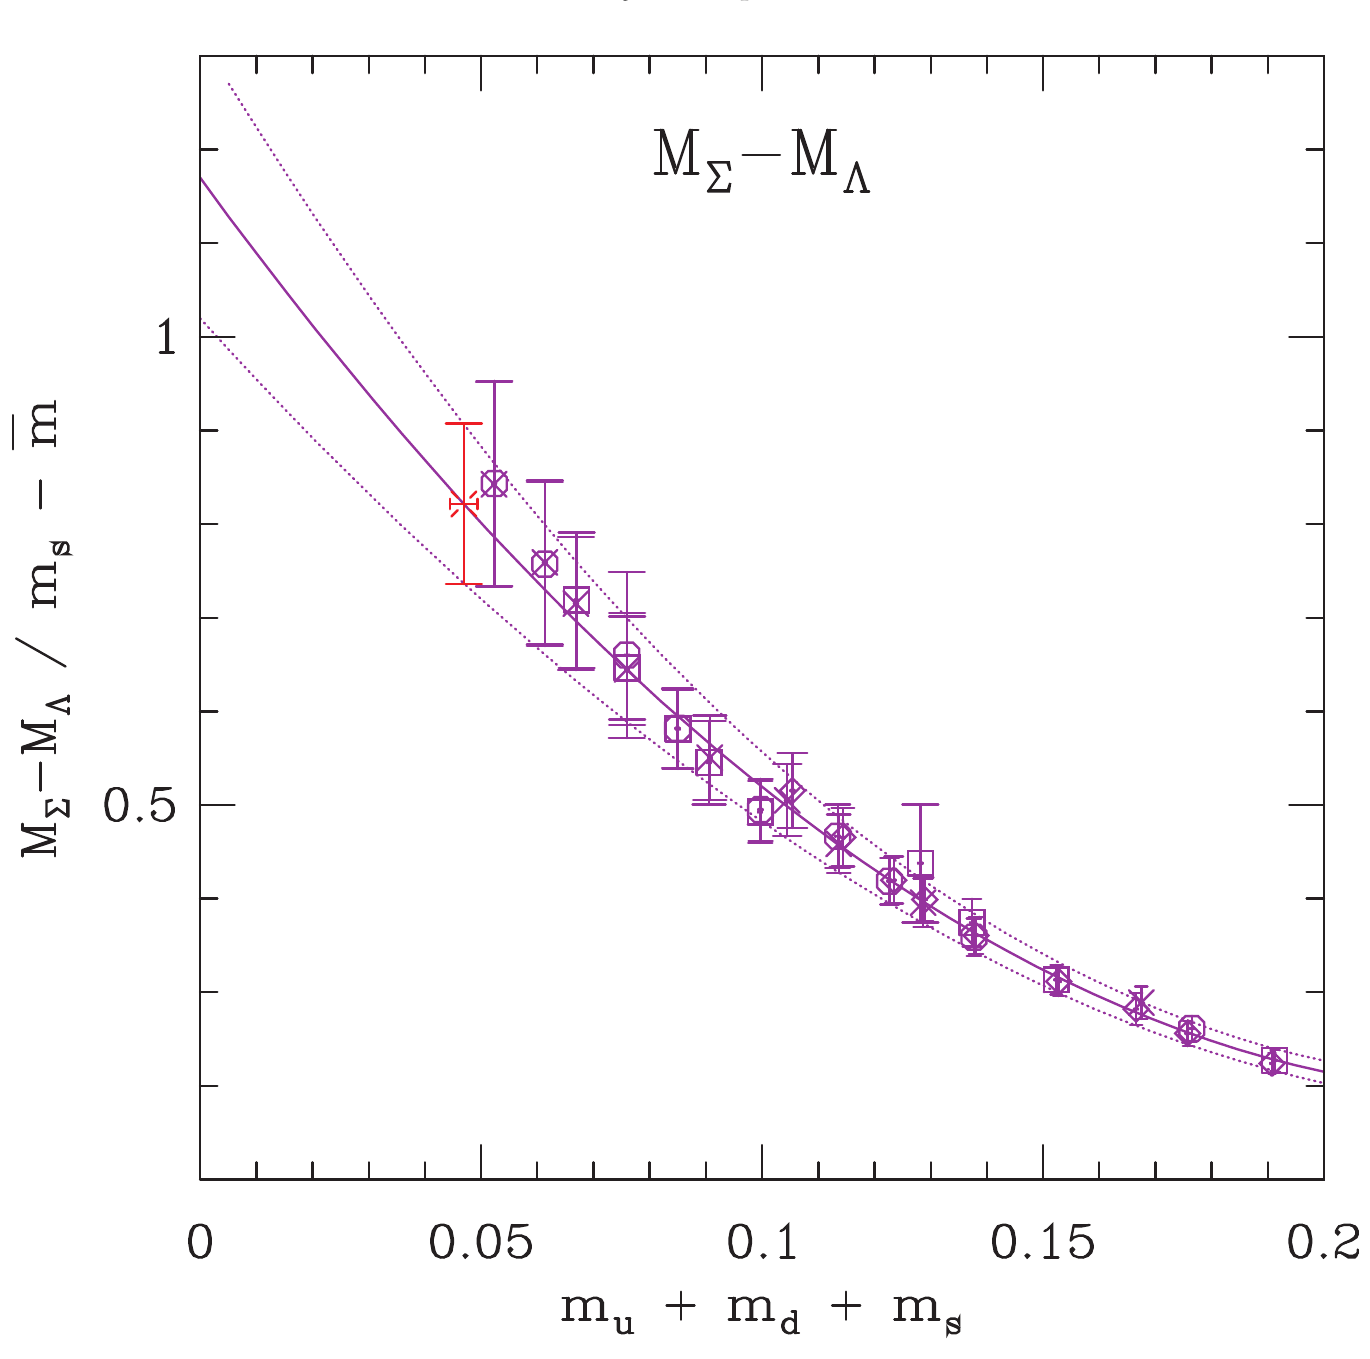
\includegraphics[width=0.8\textwidth]{images/fig27.png}
\caption{Quadratic fit to $(M_\Sigma - M_\Lambda)/(m - m_s)$, including baryons composed of completely non-degenerate quarks [156]. The value extrapolated to the physical point is shown by the burst symbol at the extreme left. The linear relations shown in Eq.~\eqref{eq:chiral} would predict a constant value.}
\label{fig:27}
\end{figure}

The non-linear terms significantly increase the splittings, and extrapolations to $m$ give results roughly consistent with experimental values. (ii) The decuplet baryon masses show a behavior linear in $m_1 + m_2 + m_3$, and the splittings come out too small for either choice $m_s(M_K)$ or $m_s(M_\phi)$.

The state-of-the-art Wilson fermion data have been obtained by the CP-PACS collaboration. Data have been obtained at four values of the lattice spacing so a reliable extrapolation to $a = 0$ can be made. Unfortunately, the data, in particular the baryon mass-splittings have not yet been fully analyzed so some of the observations presented here should be considered preliminary. Fig.~\ref{fig:28}, taken from Yoshie's review at LATTICE 97 [161], is CP-PACS's version of the chiral fits.

\begin{figure}[htbp]
\centering
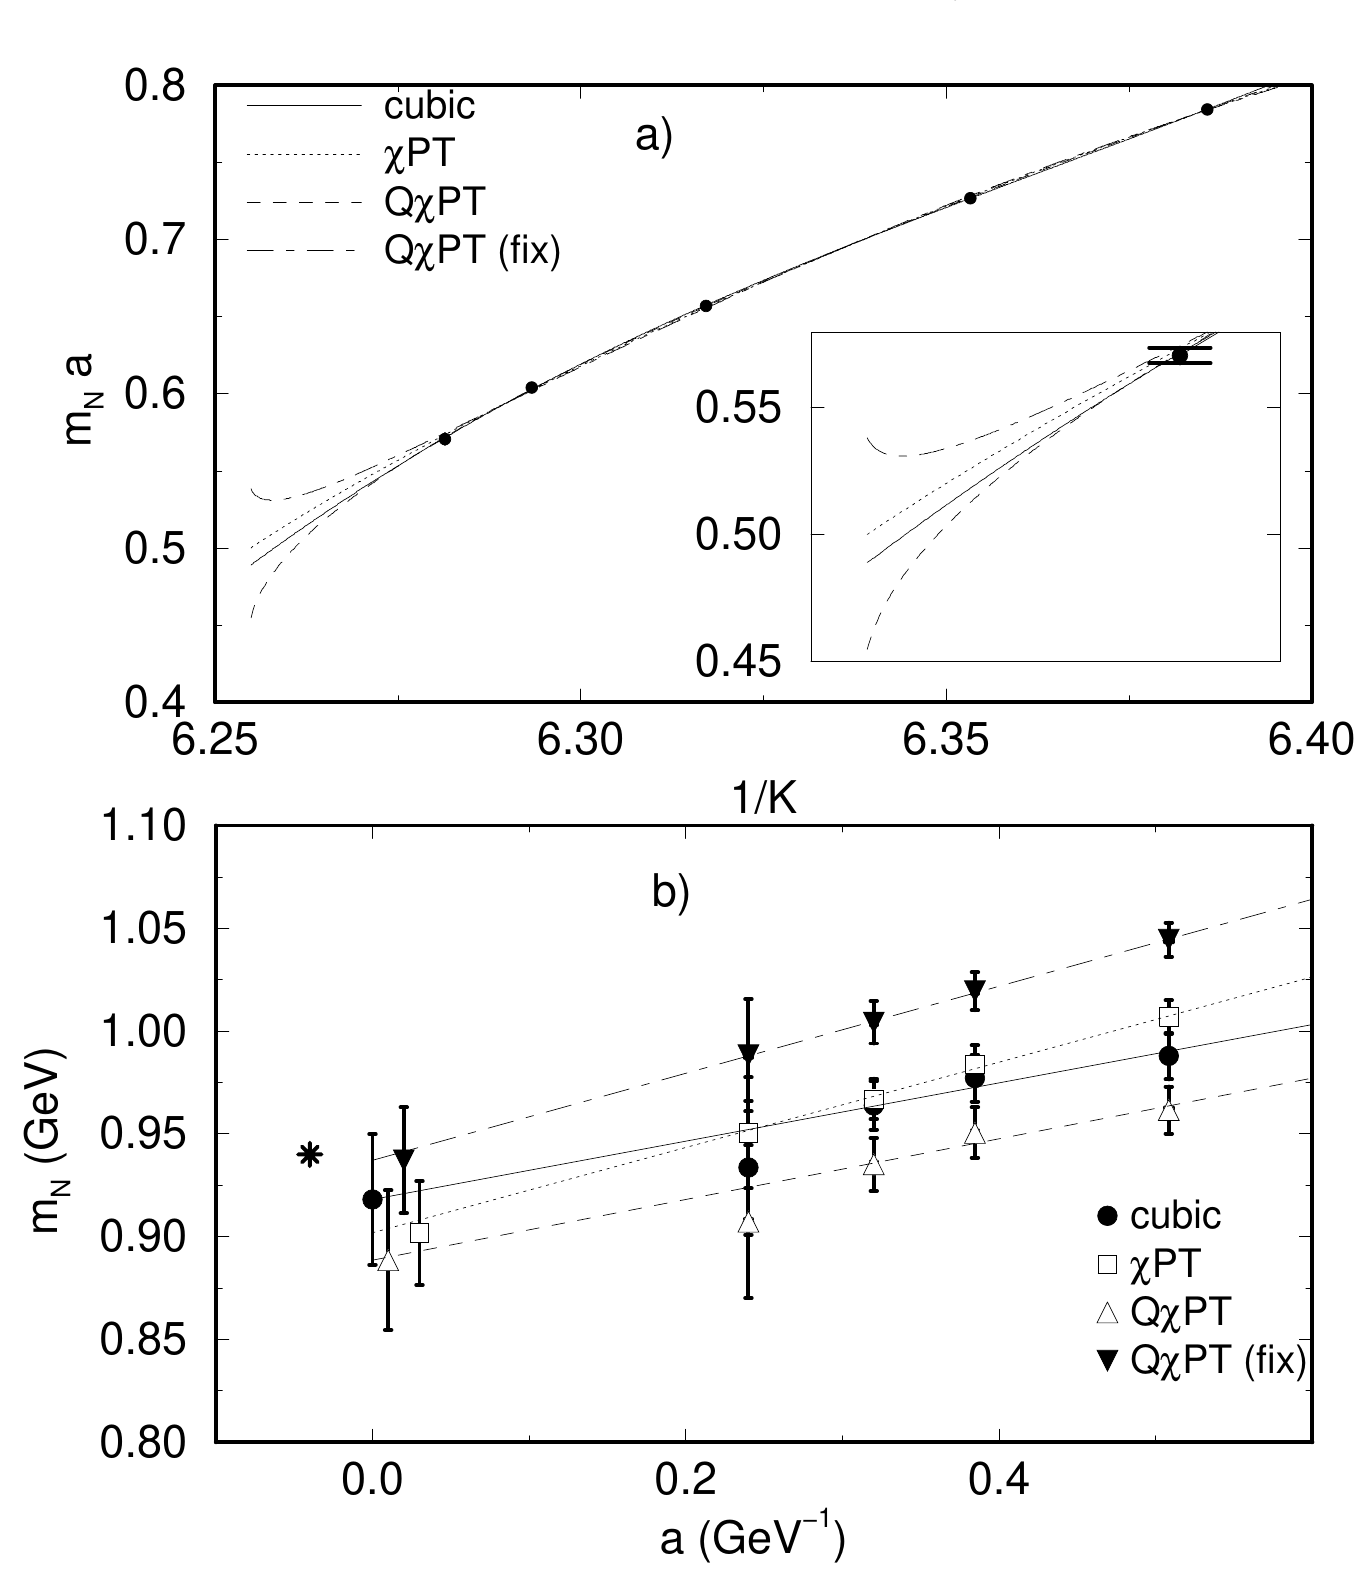
\includegraphics[width=0.8\textwidth]{images/fig28.png}
\caption{(A) Chiral fit to $M_{nucleon}$ data by the CP-PACS collaboration using the Wilson gauge and fermion actions. The data show negative curvature, though more points are needed to resolve between the cubic fit $M_N = c_0 + c_1 M_\pi + c_2 M_\pi^2 + c_3 M_\pi^3$, and $\chi$PT ($c_1 = 0$), Q$\chi$PT ($c_3 = 0$), $\chi$PT (fix) ($c_1 = -0.53$) fits. (B) Continuum extrapolation of the nucleon mass obtained using the different chiral expressions are shown in (A). The figures are reproduced from [161].}
\label{fig:28}
\end{figure}

They find that in the range $m_s/4 - m_s$ only the nucleon and the $\Lambda$ particles show any significant curvature. Even though data at more values of the quark mass are required to resolve the form of the leading higher order correction, the conclusion of their analyses is that the negative curvature found in their fits to nucleon data is sufficiently large to change the quenched estimate of $M_N / M_\rho$ to almost perfect agreement with the experimental value $\sim 1.22$. (This negative curvature was not seen/resolved in calculations reported before 1997, consequently a higher value in the range $1.3 - 1.4$ was usually reported.) Their extrapolation to $a = 0$ of results with different chiral fits is shown in Fig.~\ref{fig:29}.

\begin{figure}[htbp]
\centering
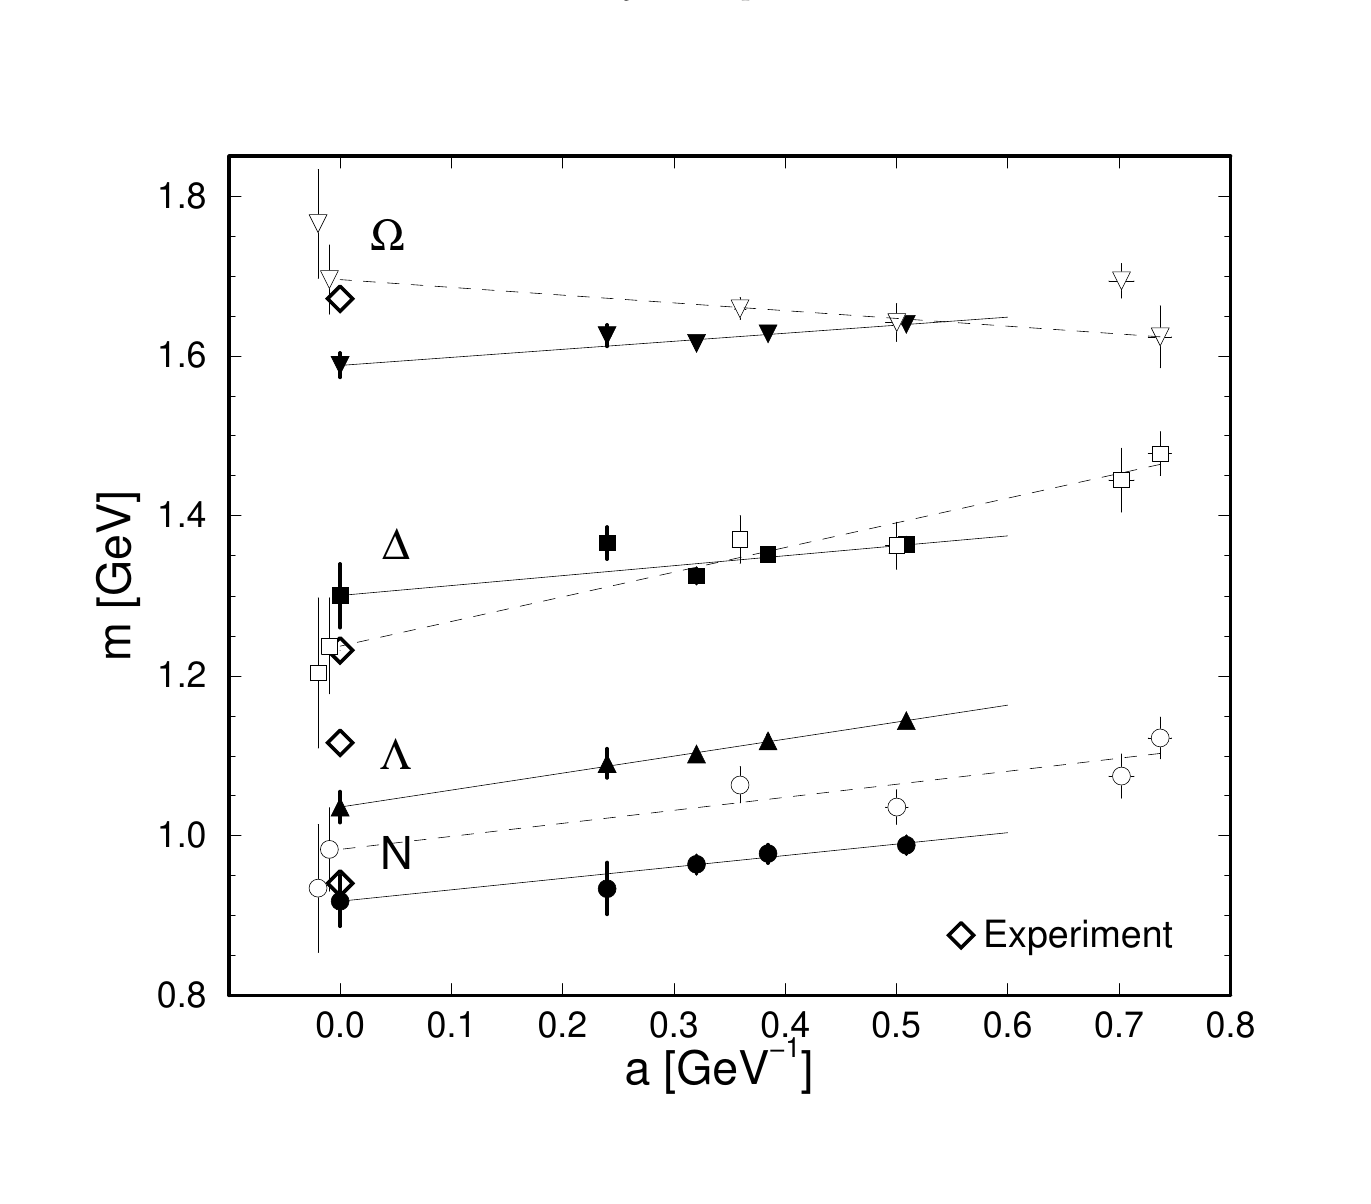
\includegraphics[width=0.8\textwidth]{images/fig29.png}
\caption{Continuum extrapolation of the nucleon, $\Lambda$, $\Delta$, and $\Omega$ masses obtained by the CP-PACS collaboration. The scale $a$ is set by $M_\rho$. The previous best results by the GF11 collaboration (unfilled symbols) are also shown. Experimental values are shown by the symbol diamond. Figure reproduced from [161].}
\label{fig:29}
\end{figure}

Second, they confirm that the decuplet masses are linear in the quark masses, and the splittings, even after extrapolation to $a = 0$, come out too small with either $m_s(M_K)$ or $m_s(M_\phi)$. Their full analyses on splittings in the baryon octet will appear soon.

A final summary of the quenched results taken from [161] using the Wilson action is given in Fig.~\ref{fig:30}.

\begin{figure}[htbp]
\centering
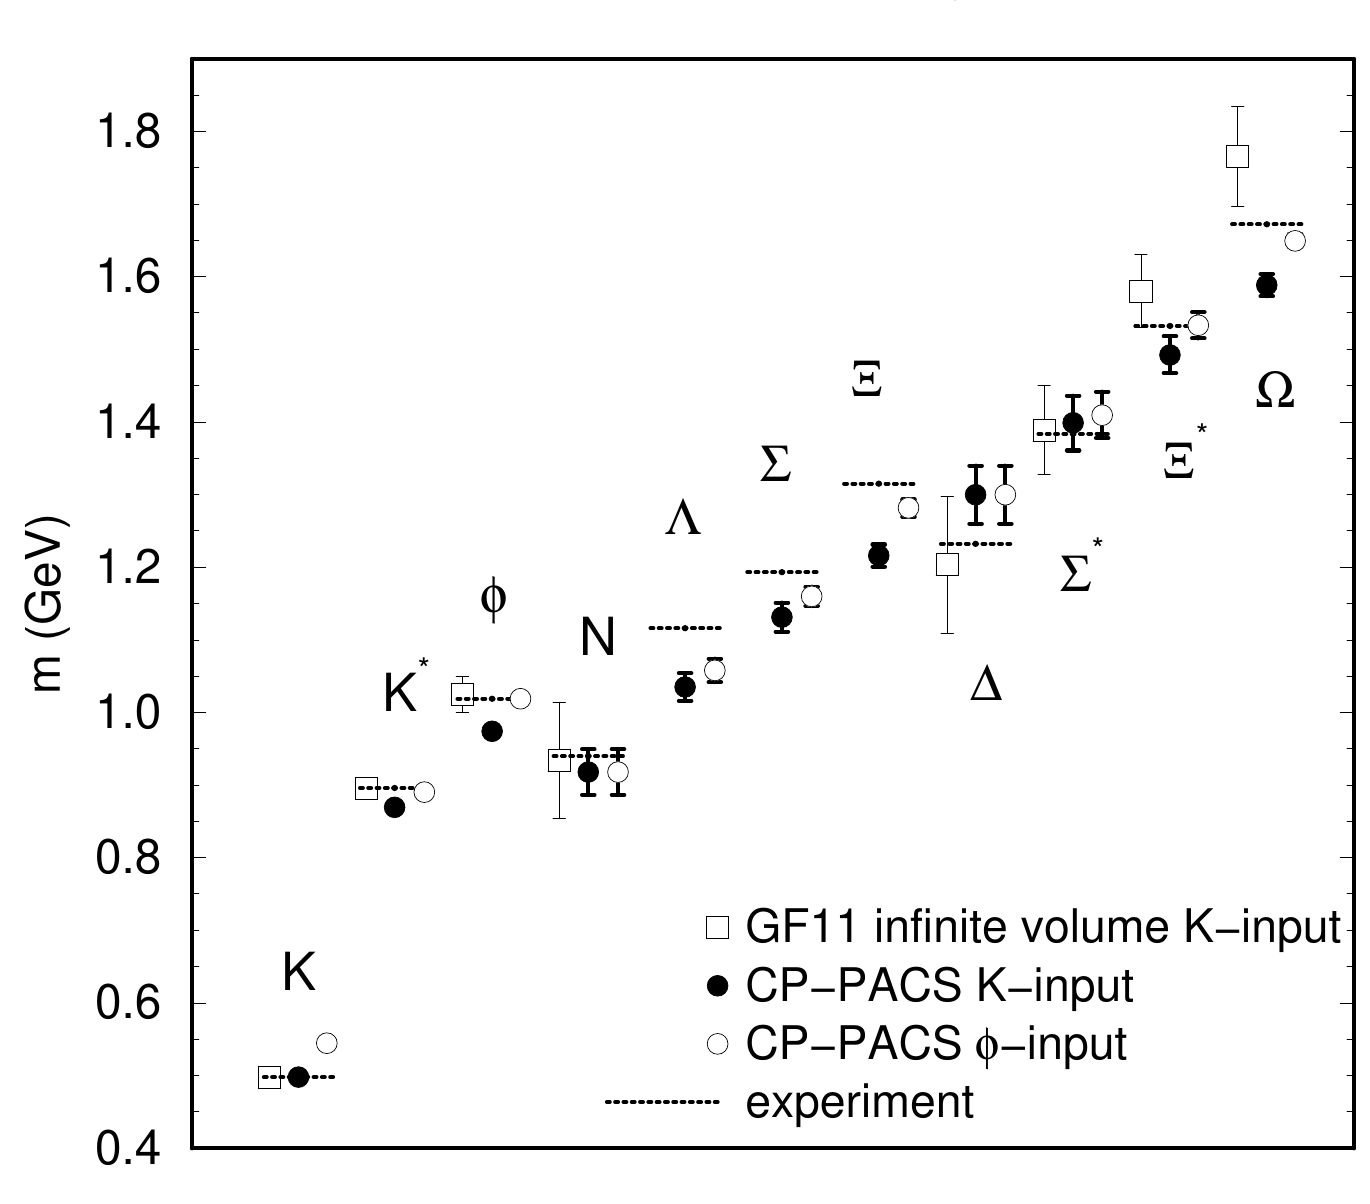
\includegraphics[width=0.8\textwidth]{images/fig30.png}
\caption{State-of-the-art results from the CP-PACS collaboration for the meson and baryon masses after $a = 0$ extrapolation and using Wilson fermions. The scale $a$ is set using $M_\rho$ and $m$ using $M_\pi$. Results are shown for two ways of setting $m_s$ --- $M_K$ and $M_\phi$ and it is clear that neither give correct splittings in the baryon octet and decuplet. The data are reproduced from [161].}
\label{fig:30}
\end{figure}

This figure compares the recent CP-PACS results extrapolated to $a = 0$ with the previous best calculation by the GF11 collaboration. The main lesson to be learned from this plot is that there does not seem to be a value of the strange quark mass that allows a matching of all the meson and baryon states. I shall come back to this point when discussing the extraction of quark masses. The obvious question is --- is this deviation an artifact of the quenched approximation? My view is that we still do not have full control over the quenched data, and therefore cannot point to quenching as the sole culprit. For example, the definition of $m_q$ itself has corrections of $O(m_q a)$, incorporating which would change the nature of the chiral fits. To fully understand the discretization errors we need to wait for similarly good quality data with the staggered and $O(a)$ improved clover formulations before claiming definitive quenched values.

As of this writing dynamical simulations have begun in earnest, but precise quantitative results at a number of values of $a$ and with different actions are lacking. Thus, I feel it is too early to draw any conclusions from them. For a status report on $n_f = 2$ results see the recent reviews by Yoshie and Gottlieb [161,160].

\section{Decay Constants}

In addition to the extraction of masses from the rate of exponential decay of the 2-point correlation function, the amplitudes $\langle n | O | 0 \rangle$ give decay constants. For example, the axial current matrix element $\langle \pi | A_\mu(x) | 0 \rangle = i f_\pi p_\mu \exp(i p \cdot x)$ gives the pion decay constant. Some of the recent results for decay constants have been reviewed by Prof.\ Martinelli at this school, and other recent reviews can be found in [163,164]. The technical points I would like to explain here are the reasons why the errors in decay constants are much larger than those in the determination of the masses. First, from Eq.~\eqref{eq:2pt} one notes that for a 1\% error in the determination of the mass, the fractional error in the decay amplitude is $\approx \exp(0.01 m \tau) - 1 \approx 0.005 m \tau$. Since fits typically have $m\tau \approx 5$ for $1/a \sim 2$ GeV lattices, the error in the decay constant is $\sim > 3\%$. Second, for any given configuration, the correlation function is highly correlated in $\tau$. Plotting $\log(\Gamma(\tau))$ for each individual configuration one notes that the dominant fluctuation is in the overall normalization, i.e., the amplitude. A very rapid growth in these fluctuations with decreasing $m_q$ is, in fact, the signal for exceptional configuration as discussed in Section~10. These two sources of error combine to produce a statistical error in decay constants that is much larger than in the extraction of $M_{eff}$. To this one has to add a systematic uncertainty coming from the renormalization constants for the local currents.

\section{Lattice Calculations of the Glueball Spectrum}

The existence of glueballs, hadronic states composed mainly of gluons, is a major untested prediction of QCD. Assuming QCD is the correct theory, we can determine the quantum numbers of a vast number of possible glueball states, but cannot yet calculate their masses, or their mixing with $q\bar{q}$, $qq\bar{q}\bar{q}$, \ldots{} states, or understand in detail the production and decay mechanisms. Various models like bag models, flux tube model, sum rules etc.\ give estimates of masses that differ significantly from each other and the reliability of these calculations is poor. A somewhat dated summary of the theoretical expectations, compiled by Burnett and Sharpe, can be found in [165]. The lack of knowledge of properties of glueballs does not help the experimentalists who have to isolate these states from the myriad of meson states in the $1-2.5$ GeV region. Clearly, LQCD calculations can play a vital role by calculating the spectrum and the mixing with $q\bar{q}$ mesons.

The first goal of LQCD has been to calculate the quenched spectrum in a world in which the mixing with quark states is turned off. I shall concentrate on just the $0^{++}$ and $2^{++}$ states as these have been studied most extensively. The glueball operators $O$ are constructed out of Wilson loops. Consider an $n \times m$ Wilson loop $W^{n,m}_{xy}$ lying in the $xy$ plane. Then the rotationally invariant sum $W^{n,m}_{xy} + W^{n,m}_{yz} + W^{n,m}_{zx}$ projects onto the $0^{++}$ state, while $W^{n,m}_{xy} - W^{n,m}_{yz}$ and its permutations project onto $2^{++}$. The signal in the 2-point correlator can be improved by taking a suitable linear combination of different sized loops that maximize the overlap with physical glueball states. One such strategy is discussed in [166]. Unfortunately, the statistical signal in glueball correlation functions is much weaker than that for meson and baryon correlation functions. Even with a sample of $O(10^5)$ independent configurations, the signal does not extend beyond $\tau \sim 10$ or $M\tau \sim 6$ and one barely has a ``plateau'' in the effective mass plot. The reason for this poor signal in glueball correlation functions is that they measure the fluctuations in the vacuum corresponding to the creation and propagation of a virtual glueball, whereas in meson and baryon correlators the quarks in the propagators are added as external sources.

The more recent, high statistics results for $M_{0^{++}}$ and $M_{2^{++}}$ states have been taken from Refs. [166--169]. The data and the extrapolation to $a = 0$ are shown in Fig.~\ref{fig:31}.

\begin{figure}[htbp]
\centering
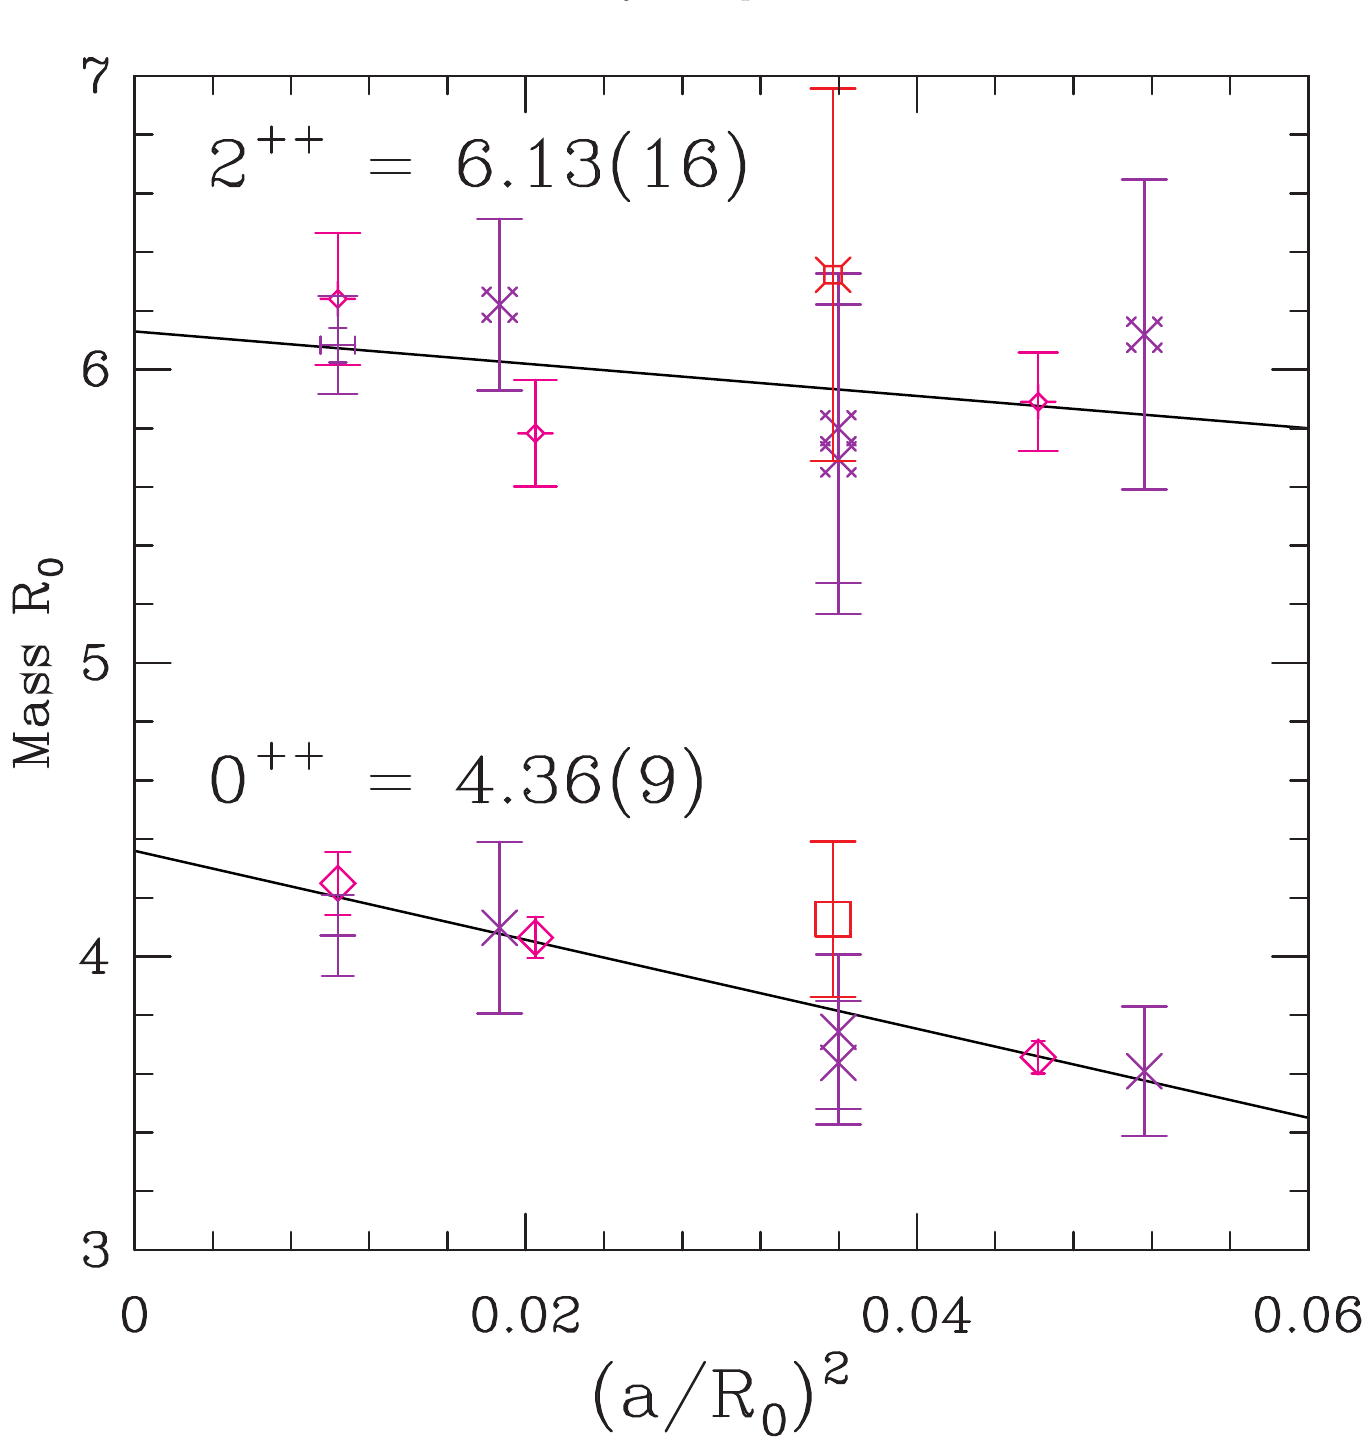
\includegraphics[width=0.8\textwidth]{images/fig31.png}
\caption{Extrapolation of $0^{++}$ and $2^{++}$ glueball mass data to $a = 0$. The data are from UKQCD-WUPPERTAL collaboration (crosses), GF11 collaboration (diamond), and Los Alamos collaboration (squares). The lattice scale is set using $R_0$ which is related to the string tension by $1/R_0 = \sqrt{\sigma}/1.18$.}
\label{fig:31}
\end{figure}

In this plot I have chosen to set the lattice scale using $R_0 = 1.18/\sqrt{\sigma}$, where $\sigma$ is the string tension [170]. The figure makes it clear that the lattice data from the various collaborations are completely consistent, though the statistical quality of the GF11 data [169] is much higher. A fit in $a^2$, the leading discretization error, gives $M_{0^{++}} R_0 = 4.36(9)$ and $M_{2^{++}} R_0 = 6.13(16)$ for the continuum limit of the quenched theory. To obtain masses in physical units one needs to choose a value for $R_0$ or equivalently $\sigma$. This brings us back to the overall scale uncertainty inherent in all quenched calculations. There are two questions relevant to this analysis (i) what value should one choose for $\sigma$, and (ii) by how much would the results change if one had used a different quantity like $M_\rho$ or $\Lambda_{QCD}$ to set the scale? The two most quoted results are the following. The UKQCD-WUPPERTAL collaboration use $1/R_0 = 373$ MeV based on choosing $\sqrt{\sigma} = 440$ MeV and get $M_{0^{++}} = 1626(34)$ and $M_{2^{++}} = 2286(60)$ MeV [170]. The updated GF11 collaboration estimates are $M_{0^{++}} = 1648(58)$ and $M_{2^{++}} = 2273(116)$ MeV using $\Lambda^{(0)}_{QCD} = 235(6)$ MeV which is based on $M_\rho$ to set the scale [171]. Thus, the estimates of the two groups are consistent and agree with the fit shown in Fig.~\ref{fig:31}. Therefore, in my view, based on these fits, the current combined lattice estimate is $M_{0^{++}} = 1640(30)(160)$ MeV and $M_{2^{++}} = 2280(60)(230)$ MeV, where I have added a second systematic error of 10\% to take into account the scale uncertainty inherent to quenched simulations.

\section{Improved action Results on Anisotropic lattices}

To alleviate the problem that the signal in glueball 2-point correlation functions falls rapidly, Peardon and Morningstar have carried out simulations on anisotropic hypercubic lattices, with $a_t \ll a_s$ [172]. The advantage of this trick is the following. Assume that there exists an approximate plateau in $M_{eff}(\tau)$ between $\tau = 2-4$ in an isotropic lattice simulation before the signal degrades to noise. Such a plateau is hard to infer from three time-slices. On the other hand for $a_s/a_t = 5$ lattices, one has roughly 11 time-slices to play with, thereby greatly increasing the confidence in the estimate. Using anisotropic lattices does introduce an additional parameter into the analyses, $a_s/a_t$ or the velocity of light. This they fix non-perturbatively using the measured potential in spatial and temporal directions.

\begin{figure}[htbp]
\centering
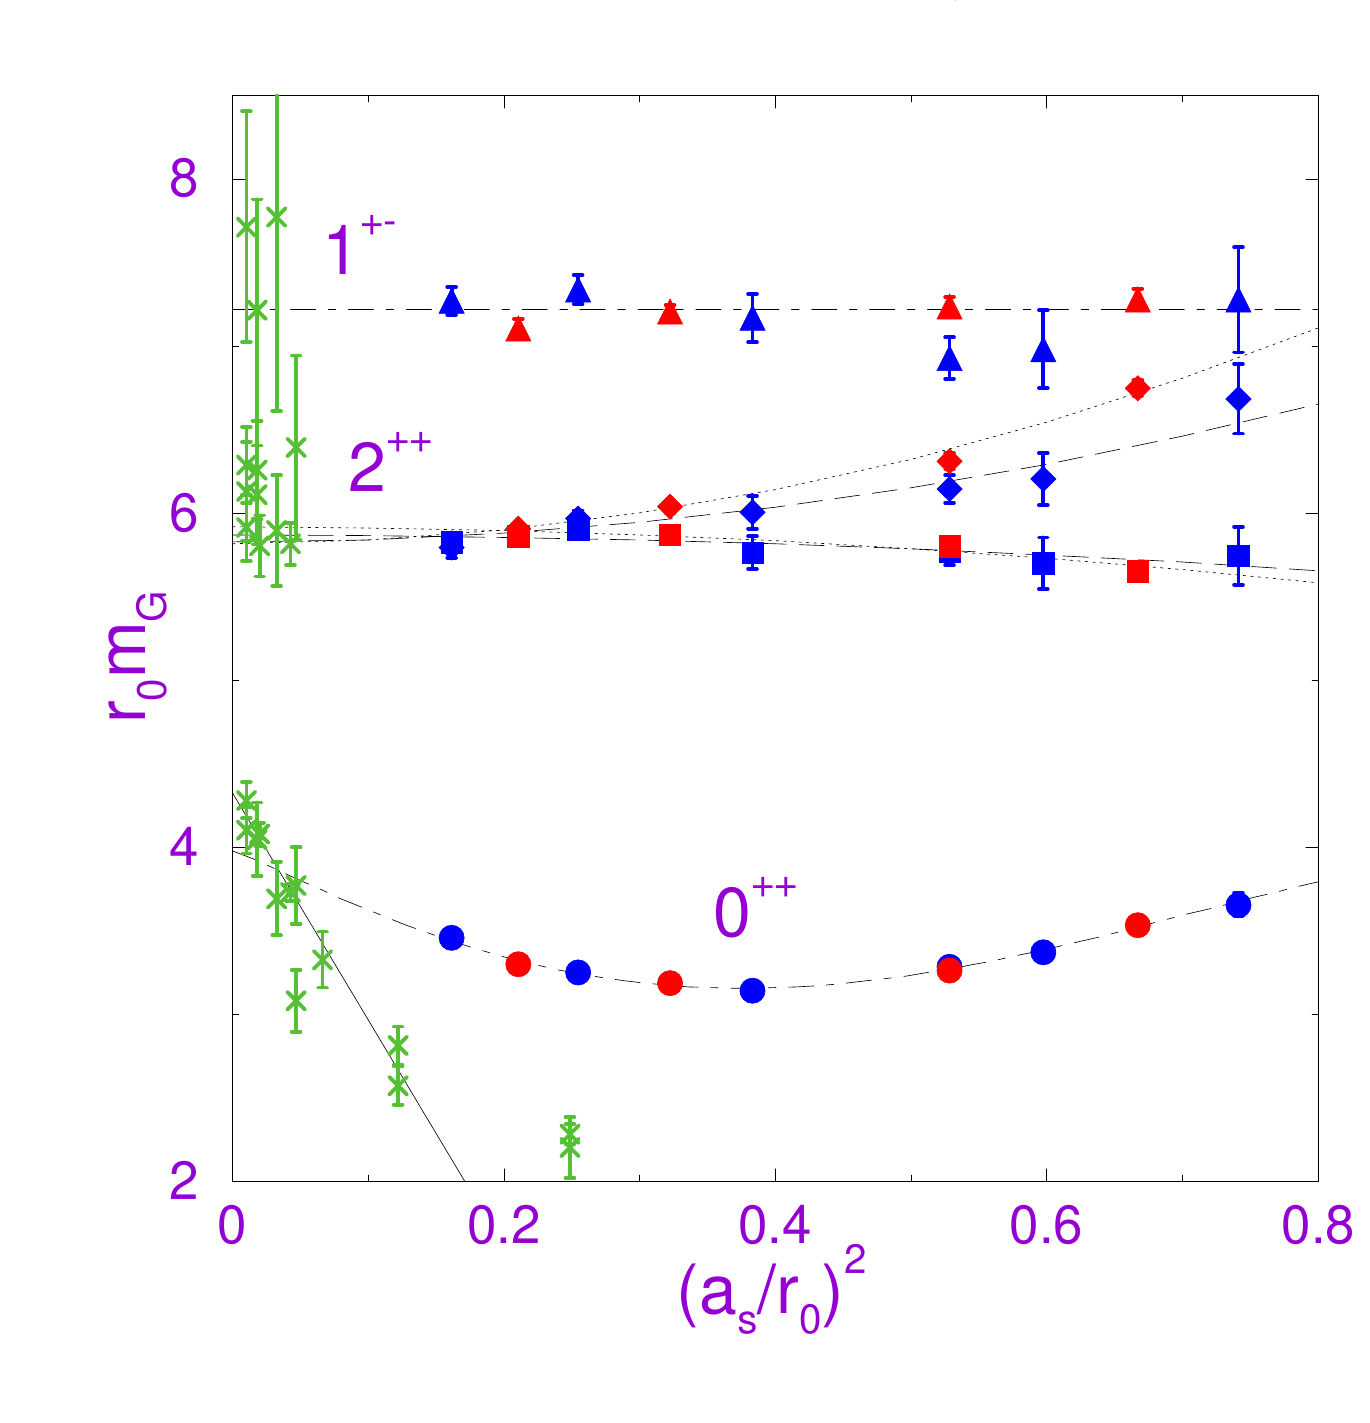
\includegraphics[width=0.8\textwidth]{images/fig32.png}
\caption{Glueball mass estimates in terms of $R_0$ against the lattice spacing $(a_s/R_0)^2$. Results from the $\xi = 5$ simulations for the lattice irreps $A_1^{++}$ ($0^{++}$), $E^{++}$, $T_2^{++}$ ($2^{++}$), and $T_1^{+-}$ ($1^{+-}$) are labeled $\circ$, $\square$, $\star$, and $\triangle$ (blue), respectively. The corresponding symbols in red indicate the results from the $\xi = 3$ simulations. Data from Wilson action simulations taken from Refs. [167--169] are shown using green crosses. The dashed, dotted, and dash-dotted curves indicate extrapolations to the continuum limit obtained by fitting to the $\xi = 3$ data, the $\xi = 5$ data, and all data, respectively. The solid line indicates the extrapolation of the Wilson action data to the continuum limit.}
\label{fig:32}
\end{figure}

The second improvement they make is to tune the action. They transcribe the tadpole improved L\"uscher-Weisz glue action, Eq.~12.14, on to anisotropic lattices and include the plaquette in both the fundamental and adjoint coupling space. The motivation for the latter is to avoid the phase transition in the fundamental-adjoint space as discussed in Section~15.

Their new data [139] confirms that including a negative adjoint coupling does improve the scaling in $M_{0^{++}}$.

Their results, prior to those including a negative adjoint coupling, are shown in Fig.~\ref{fig:32}. The advantage of improved action and anisotropic lattices is clearly visible. First, the calculations can be performed on much coarser lattices. Second, the discretization errors are much smaller. Lastly, the values after extrapolation to $a = 0$ are consistent with conventional methods. Their estimates $M_{0^{++}} R_0 = 3.98(15)$ and $M_{2^{++}} R_0 = 5.85(2)$, when combined with their estimate $R_0 = 410(20)$ MeV, are consistent with the values from conventional simulations given in the previous section. Thus, their results provide another confirmation of the quenched estimates.

Let me end this discussion of gluey states with pointers to other interesting calculations. Results for other spin-parity glueball states can be found in [168,172,173]; and for hybrid states in [173--176].

\section{Mixing between scalar quarkonia and glueballs}

The phenomenologically important question is whether the lattice estimates can help pin down which of the two experimental candidates, $f_0(1500)$ or $f_0(1710)$, is the scalar glueball. The answer, using just the above quenched estimates, is no. The reason, in addition to the fact that the above estimates overlap with both candidates, is that effects of mixing with scalar quarkonia have not been included. Lee and Weingarten have initiated a study of mixing by calculating the two-point functions $\langle S(\tau) S(0) \rangle$ and $\langle G(\tau) S(0) \rangle$ where $S$ is the scalar density $(u\bar{u} + d\bar{d})/\sqrt{2}$ or $s\bar{s}$ and $G$ is the $0^{++}$ glueball operator [171]. The statistical quality of these very hard calculations is not yet good. Lee and Weingarten, therefore, diagonalize an approximate $3 \times 3$ matrix that is obtained mainly from a phenomenological analysis. They then find that mixing raises $M_{0^{++}}$ by $\sim 64$ MeV, i.e.\ $M_{0^{++}}$ changes from 1640 to 1704 MeV. Also, the associated wavefunctions of the mixed states explain some of the unexpected features of decays, like why the $KK$ decay mode of $f_0(1500)$ is suppressed and why $\Gamma(J/\psi \to \gamma f_0(1710)) > \Gamma(J/\psi \to \gamma f_0(1390)) \gg \Gamma(J/\psi \to \gamma f_0(1500))$. Consequently, Lee and Weingarten predict that $f_0(1710)$ is dominantly ($\sim 75\%$) a glueball.

In obtaining these predictions, they neglected mixing with other (multiparticle) states and decay widths in the mixing matrix and quenching errors in the lattice calculations. These, Lee and Weingarten claim on the basis of phenomenological arguments, are small and do not change their central conclusion. Hopefully, future LQCD calculations will provide a much better quantitative validation of their prediction.

\section{Mass Inequalities}

In addition to getting hard numbers, LQCD (actually Euclidean field theory) has also prompted the derivation of rigorous mass-inequalities. The first such was derived by Weingarten showing that the pion is the lightest meson state of non-zero isospin in QCD [177]. Consider the 2-point correlation function for mesons, i.e.\ $O = \bar{u}\Gamma d$ where $\Gamma$ can be any one of the 16 elements of the Clifford algebra. Then
\begin{equation}
\begin{aligned}
\Gamma_{\Gamma}(\tau) &= \int d^3y\, \langle 0 | \bar{d}\Gamma u(\tau, y)\, \bar{u}\Gamma d(0, x) | 0 \rangle \\
&= \Tr\, S_F^d(0,x;\tau,y)\,\Gamma S_F^u(\tau,y;0,x)\,\Gamma \\
&= \Tr\, \Gamma\gamma_5 S_F^{d\dagger}(\tau,y;0,x)\,\gamma_5 \Gamma S_F^u(\tau,y;0,x).
\end{aligned}
\label{eq:18.4}
\end{equation}

For the special case of the pion, $\Gamma\gamma_5 = 1$, consequently $\Gamma_\pi(\tau)$ has the maximum value on each configuration. Furthermore, for $m_u = m_d$ it is the absolute square of the propagator. The other spin-parity states involve $\gamma$ matrices. Since these have both plus and minus signs, the various spinor terms in the trace have cancellations. The second property needed to translate this property of correlation functions into an inequality on masses is that the integration measure for QCD is positive, i.e.\ each configuration contributes with the same sign. Thus, $\Gamma_\pi(\tau) \ge \Gamma_\Gamma(\tau)$ for all $\tau$. Since, $\Gamma(\tau) \sim e^{-m\tau}$, the inequality implies that the pion is the lightest meson.

Concurrently, Witten and Nussinov derived further inequalities. Examples of these are
\begin{itemize}
  \item The electromagnetic mass shift in the pion is positive [179]. Specifically what is shown is that $V_\mu^3(k)V_\mu^3(-k) - A_\mu^3(k)A_\mu^3(-k) \ge 0$ for any Euclidean $k$.
  \item For mesons with valence flavors $A$ and $B$ the inequality $2M_{AB} \ge M_{AA} + M_{BB}$ holds in the limit that annihilation into gluonic states can be neglected in the flavor singlet correlators [179,178].
\end{itemize}

Recently West has applied/extended these methods to glueballs [181]. He shows that $0^{++}$ is the lightest glueball state.

\chapter{The strong coupling constant $\alpha_s$}

Spectroscopy studies, in addition to testing QCD, allow the determination of some of the fundamental parameters of the SM, i.e., the coupling $\alpha_s$ and the quark masses. To determine $\alpha_s$, one needs to know not only its strength but also the energy scale $Q$ at which the coupling is measured. The calculation of $\alpha_s$, in general, proceeds as follows. One chooses a quantity $O$ that can be measured very accurately, either in high energy experiments or via non-perturbative methods on the lattice, and for which a perturbative expansion is known, i.e.,
\begin{equation}
O = \sum_n A_n \alpha_s^n(Q),
\end{equation}
where the $A_n$ are the perturbative coefficients. Inverting this relation gives $\alpha_s(Q)$.

One promising lattice approach for calculating $\alpha_s$ has been pioneered by the NRQCD collaboration [110]. They examine several short-distance $O$, like the expectation value of small Wilson loops, that can be calculated very accurately on the lattice and for which perturbative expansions are known to at least $O(\alpha_s^2)$. The scale $Q$ characterizing these lattice observable is typically of the form $Q = C/a$ where $a$ is the lattice spacing and $C$ is a constant that needs to be fixed. They determine $C$ relevant to $O$ by evaluating the mean momentum flow in the perturbative expressions for these quantities. The scale $1/a$ is fixed using level splittings in quarkonia. In particular they use the spin-averaged S-P and the 1S-2S splittings in the Upsilon system. The advantage of using these splittings is that they show negligible sensitivity to the precise tuning of the bottom quark mass, and the corrections due to light quark loops are expected to be small.

Finally, to convert from $\alpha_s$ in the lattice scheme to $\alpha_{\overline{\mathrm{MS}}}$ they use the two loop relation, and include reasonable estimates of the $\alpha_s^3$ term in the error analysis. Their final estimate
\begin{equation}
\alpha_{\overline{\mathrm{MS}}}(M_Z) = 0.1174(24)
\end{equation}
includes quenching uncertainties. This remarkably precise result is consistent with the world average of experimental determinations, $\alpha_s = 0.118(3)$, as shown in Fig.~\ref{fig:33}.

An alternate method for measuring $\alpha_s$ has been carried out by the ALPHA collaboration [182]. In their method, called the Schr\"odinger functional approach, $\alpha_s$ is defined by measuring the response of the lattice system to an external field. They fix the lattice scale $a$ using the force at some fixed distance ($R_0 = 0.5$ fermi). They evolve their coupling to a very high scale using a non-perturbative renormalization group stepping procedure. At this high scale they define $\Lambda^{(0)}_{\overline{\mathrm{MS}}}$ using the two loop relation and include the three loop uncertainty, which is small, in error estimates. They have completed the calculation for the quenched theory with the result $\Lambda^{(0)}_{\overline{\mathrm{MS}}} = 251(21)$~MeV, and are now doing the $n_f = 2$ simulations [182]. The corresponding value $\alpha_{\overline{\mathrm{MS}}}(90~\mathrm{GeV}) = 0.0818(10)$ is lower than in nature. This difference is attributed to having neglected sea quark effects.

\begin{figure}[htbp]
\centering
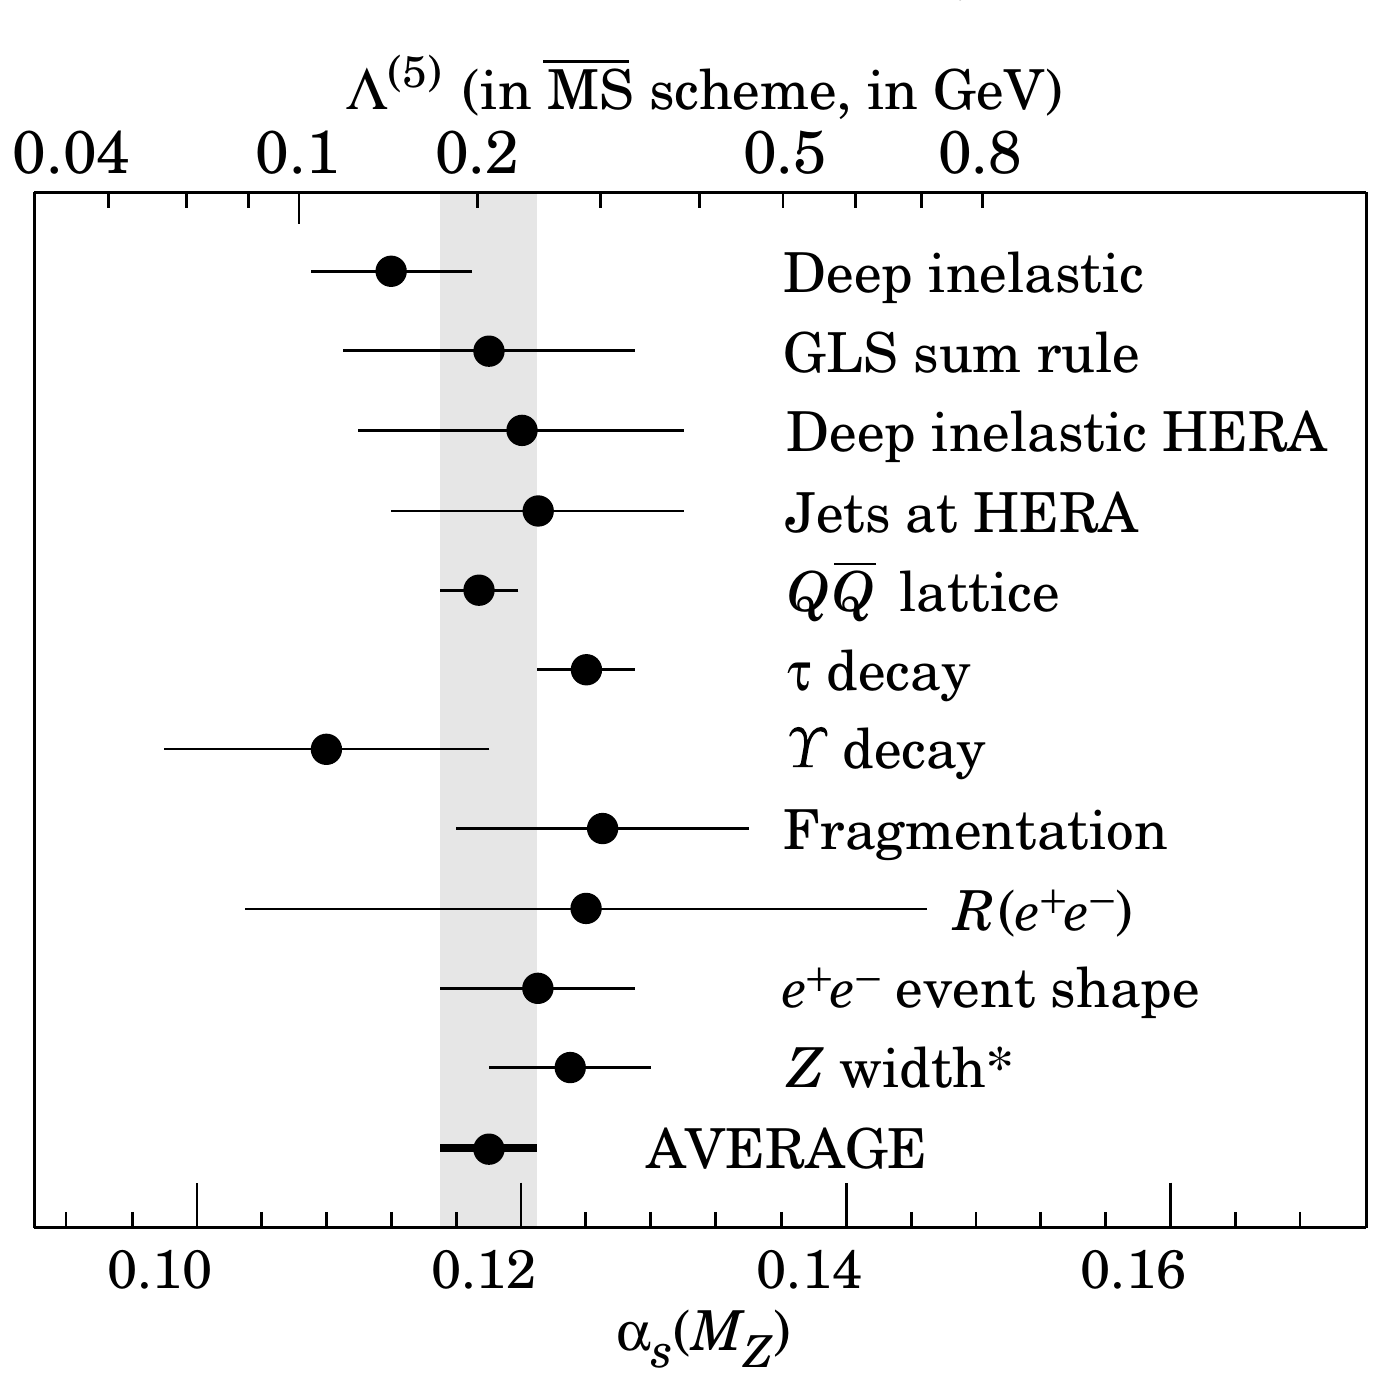
\includegraphics[width=0.8\textwidth]{images/fig33.png}
\caption{Summary of the values of $\alpha_s(M_Z)$ and $\Lambda^{(5)}$ (the QCD scale for 5 active quark flavors) extracted from various processes. These are ordered from top to bottom by increasing energy scale of measurements. This figure is reproduced from the 1996 Review of Particle Physics, updated to show the latest lattice result, $\alpha_{\overline{\mathrm{MS}}}(M_Z) = 0.1174 \pm 0.0024$. It is a remarkable confirmation of QCD that the $\alpha_s$ extracted from processes at different scales has the same value.}
\label{fig:33}
\end{figure}

A similar low value is obtained in the NRQCD analyses if no corrections are made for the quenched approximation. For details of the Schr\"odinger functional method see the lectures by Prof.~L\"uscher at this school.

\chapter{Quark Masses}

Quarks are not asymptotic states of nature, so their masses cannot be measured in experiments. They are generally defined in some perturbative scheme like $\overline{\mathrm{MS}}$ and at some scale $\mu$. Their values remain amongst the least well known of the Standard Model parameters. In this section I will discuss their extraction from lattice data.

The extraction of the up, down, and strange quark masses from the hadron spectrum is done by inverting Eqs.~18.3 once the coefficients $A_\pi$ etc.\ are determined from fits to the lattice data. As I have mentioned before, current lattice simulations neglect iso-spin breaking effects, so we can only determine $m = (m_u + m_d)/2$ and $m_s$. I will discuss these first and then briefly mention the extraction of the heavy quark masses $m_c$ and $m_b$.

In the quenched approximation, the most straightforward way to estimate $m$ is to extrapolate $M_\pi^2/X^2$ to the physical value. Here $X$ is a dimensionful quantity like $f_\pi$ or $M_\rho$ or $M_N$ or $M_\Delta$ that does not depend on $m_s$, and de facto sets the lattice scale $1/a$. Of the above quantities, using $M_\rho$ is the most controversial as it decays via strong interactions and has a large width, 170~MeV. On the other hand the lattice data for $M_\rho$ is most readily available and has good signal. Also, in the quenched approximation the $\rho$ does not decay. Using $M_\rho$ to set $a$ in QQCD versus some other quantity can therefore give an overall scale uncertainty. The spread in $1/a$ extracted from different quantities is found to be $\approx 10\%$, and this uncertainty, inherent to the quenched approximation, will be treated as an overall systematic error. Similarly, one can set $m_s$ by extrapolating the ratio $M_s/X$, where $M_s$ is any state that depends on $m_s$ like $M_K$, or $M_{K^*}$, or $M_\phi$ or any of the baryons containing a strange quark. The world data show that different choices of $M_s$ give rise to a $\approx 20\%$ spread in $m_s$. It is important to note that if one assumes the relation $M_{PS}^2 = B_{PS} m_q$ (which LQCD has not validated as true for the whole range $[m, m_s]$), and uses $M_K$ to fix $m_s$, then the ratio $m_s/m$ has to be 25.9 if $m$ is set using $M_\pi^2$.

In the full theory $X$ depends on $m_s$, and similarly $M_s$ depends on $m$, through sea quark effects. Thus, $m$, $a$, and $m_s$ have to be fixed by solving the coupled set of equations.

Simulations of the hadron spectrum have been done by a number of collaborations around the world, and there exists a large amount of data for the masses of hadrons as a function of the quark masses and lattice spacing. (Almost all lattice collaborations, for example the APE, Columbia University, CP-PACS, Fermilab, GF11, HEMCGC, JLQCD, Los Alamos, SCRI, staggered, UKQCD, and the Wuppertal University collaborations, have contributed to these calculations [183].) In early analyses the estimates of quark masses varied by almost a factor of two between different formulations of fermions, and the pattern of the discretization and quenching errors was not obvious from the work of any one collaboration. Clarification of this issue has been obtained by putting together all the world data for Wilson, clover, and staggered fermions [183,184]. The final picture for $m$, based on the most recent, high statistics, and large lattices data is shown in Fig.~\ref{fig:34} for the three fermion formulations. This figure shows clearly that the factor of $\sim 2$ difference at $1/a \sim 2$~GeV shrinks to $\sim 15\%$ after extrapolation to $a = 0$, i.e.\ most of the difference can be explained as due to discretization errors.

The behavior of $m_s$ versus $a$ is very similar. A summary of the quenched results in MeV at scale $\mu = 2$~GeV, based on an analysis of the 1997 world data [185], is

\begin{table}[htbp]
\centering
\begin{tabular}{lccc}
\toprule
          & $m(M_\pi)$ & $m_s(M_K)$ & $m_s(M_\phi)$ \\
\midrule
Wilson    & 4.1(1)     & 107(2)     & 139(11)       \\
TI Clover & 3.8(1)     & 99(3)      & 117(8)        \\
Staggered & 3.5(1)     & 91(2)      & 109(5)        \\
\bottomrule
\end{tabular}
\caption*{Quenched estimates of the light quark masses (in MeV), at scale $\mu = 2$~GeV, for the Wilson, tadpole improved clover (TI Clover), and staggered formulations of fermions, based on an analysis of the 1997 world data [185].}
\label{tab:light-quark-masses}
\end{table}

These estimates were obtained using the following Ans\"atze.
\begin{itemize}
\item Chiral fits were made keeping only the lowest order terms shown in Eqs.~18.3.
\item $M_\pi^2/M_\rho$ is used to fix $m$.
\item Results for $m_s$ are given for two choices, $M_K^2/M_\rho$ and $M_\phi/M_\rho$. (Using $M_{K^*}/M_\rho$ gives values almost identical to those with $M_\phi/M_\rho$. This implies that for the choice $m_s(M_\phi)$ one could equivalently have set the scale using $M_{K^*}$ instead of $M_\rho$.)
\item Since linear chiral fits have been used, $m_s(M_K) \equiv 25.9\,m$.
\item The matching factor, $Z_m$, between lattice and $\overline{\mathrm{MS}}$ schemes is the tadpole improved 1-loop result.
\item The extrapolation to $a = 0$ is done using the lowest order discretization error, i.e.\ $O(a)$ and $O(\alpha_s a)$ for Wilson and clover, and a quadratic in $a^2$ for staggered.
\end{itemize}

The final difference in estimates between Wilson, tadpole improved clover (TI Clover), and staggered results is $\approx 15\%$ as shown in Fig.~\ref{fig:34}. This could be due to the neglected higher order discretization errors and/or due to the difference between non-perturbative and 1-loop estimates of $Z$'s. Similarly, the $\approx 20\%$ variation in $m_s$ with the state used to extract it, $M_K$ versus $M_\phi$ (or equivalently $M_{K^*}$) could be due to the quenched approximation or partly an artifact of keeping only the lowest order discretization correction in the extrapolations. To disentangle these discretization and quenching errors requires precise unquenched data with roughly physical values for light quarks.

\begin{figure}[htbp]
\centering
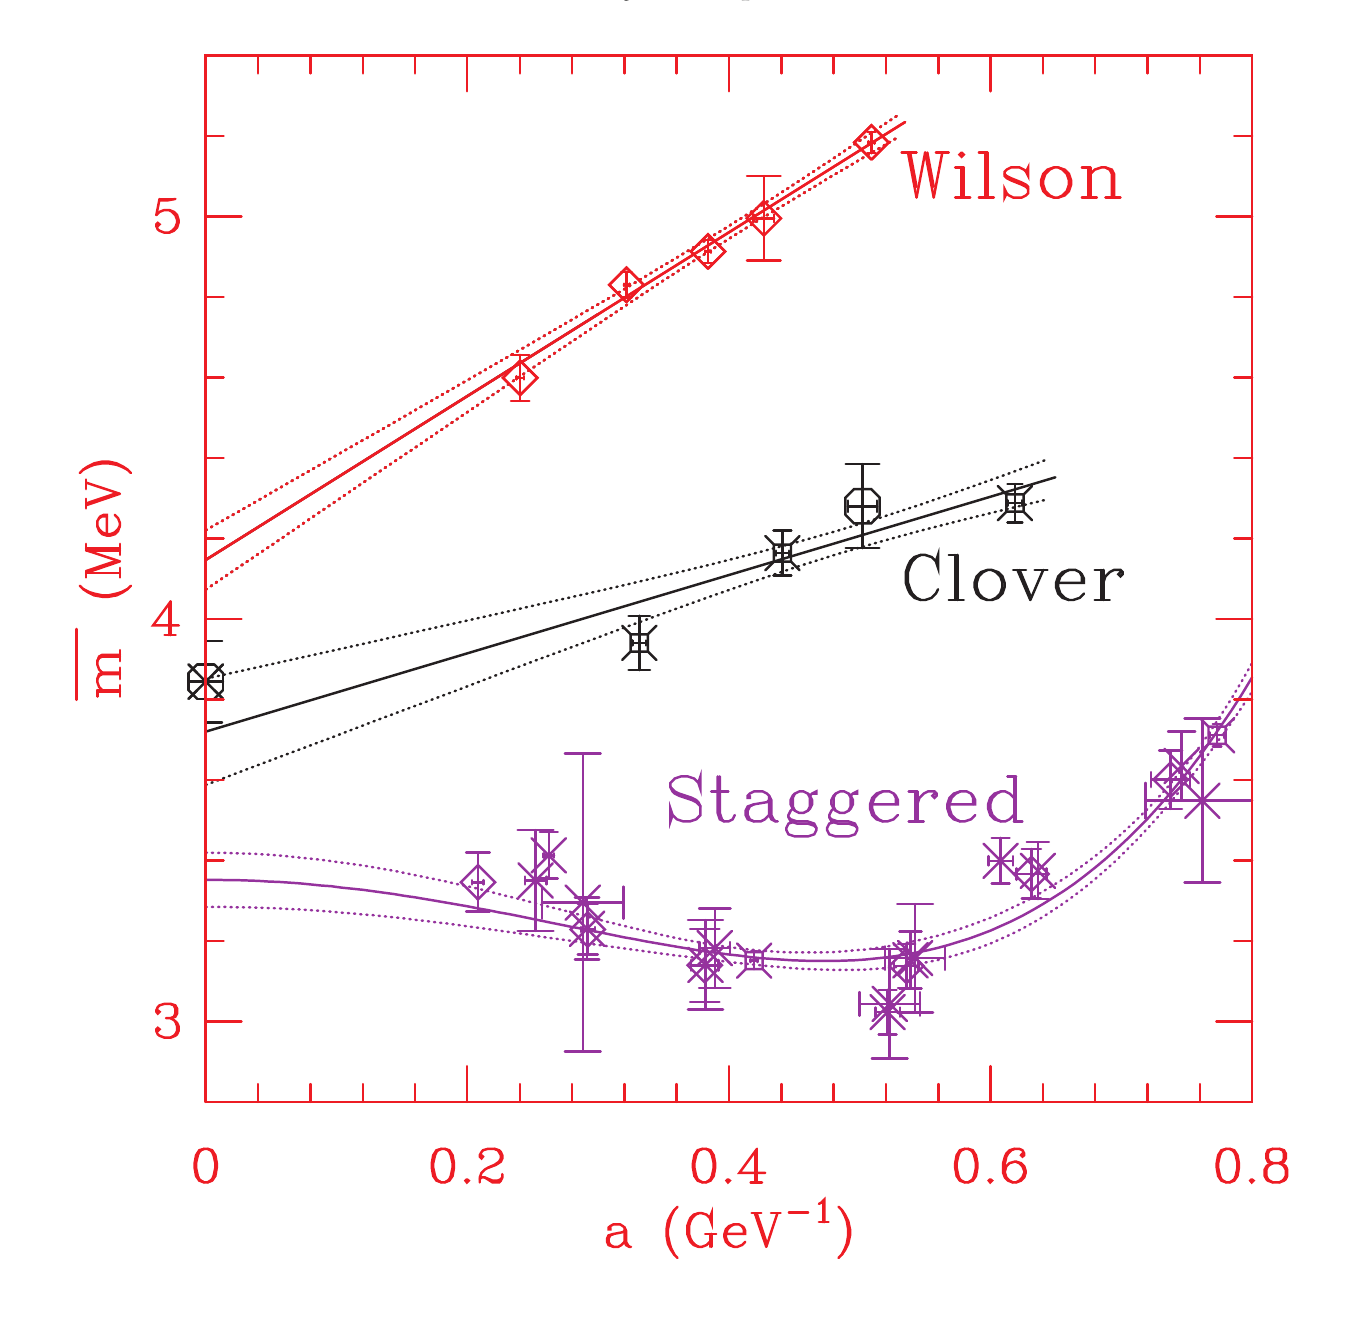
\includegraphics[width=0.8\textwidth]{images/fig34.png}
\caption{The behavior of $m_u + m_d$ as a function of the lattice spacing $a$ for three discretization schemes -- Wilson, clover, and staggered. Linear extrapolations to $a = 0$ are shown for Wilson and clover formulations, while for staggered both $O(a^2)$ and $O(a^4)$ terms are incorporated in the fit. The theoretically expected form for discretization errors in the clover formulation is $O(\alpha_s a)$. The extrapolated value using this form is shown by the symbol burst.}
\label{fig:34}
\end{figure}

For best estimates of quenched results I average the data and use the spread as the error. To these, I add a second systematic error of 10\% due to the uncertainty in the determination of the scale $1/a$, which partly reflects the uncertainty due to the quenched approximation. The results, in the $\overline{\mathrm{MS}}$ scheme and evaluated at 2~GeV, are [185]
\begin{equation}
\begin{aligned}
m &= 3.8(4)(4)~\mathrm{MeV}, \\
m_s &= 110(20)(11)~\mathrm{MeV}.
\end{aligned}
\end{equation}

\section{Light Quark Masses from Ward Identities}

A second method for extracting quark masses is based on axial and vector current Ward identities
\begin{equation}
\begin{aligned}
Z_A\,\partial_\mu A_\mu &= (m_1 + m_2)_R\, Z_P\, P, \\
Z_V\,\partial_\mu V_\mu &= (m_1 - m_2)_R\, Z_S\, S,
\end{aligned}
\end{equation}
where 1, 2 are the flavor indices and $P$ and $S$ are the lattice pseudoscalar and scalar densities. From these one can construct ratios of 2-point correlation functions
\begin{equation}
\begin{aligned}
\frac{Z_P}{Z_A}\,\frac{\langle \partial_\mu A_\mu(\tau)\,P(0)\rangle}{\langle P(\tau)P(0)\rangle} &= (m_1 + m_2)_R, \\
\frac{Z_S}{Z_V}\,\frac{\langle \partial_\mu V_\mu(\tau)\,S(0)\rangle}{\langle S(\tau)S(0)\rangle} &= (m_1 - m_2)_R,
\end{aligned}
\end{equation}
which give the renormalized quark masses once the various renormalization constants $Z_i$ are known. Since the Ward identities are operator identities, Eq.~20.3 holds for all $\tau$ except at very short times where there is influence of contact terms. Thus it is not necessary for the signal to persist to asymptotic $\tau$ as needed in spectroscopy method to isolate the lowest state.

The two estimates of quark masses, from spectroscopy and from the Ward identities, should agree in the continuum limit. A comparison of the two data sets for the Wilson action and using 1-loop perturbative $Z$'s is shown in Fig.~\ref{fig:35}. The two estimates are significantly different at finite $a$, however, a linear extrapolation works for both sets of data, and the extrapolated values are in surprisingly good agreement. One could therefore attribute the differences at finite $a$ to discretization errors.

\begin{figure}[htbp]
\centering
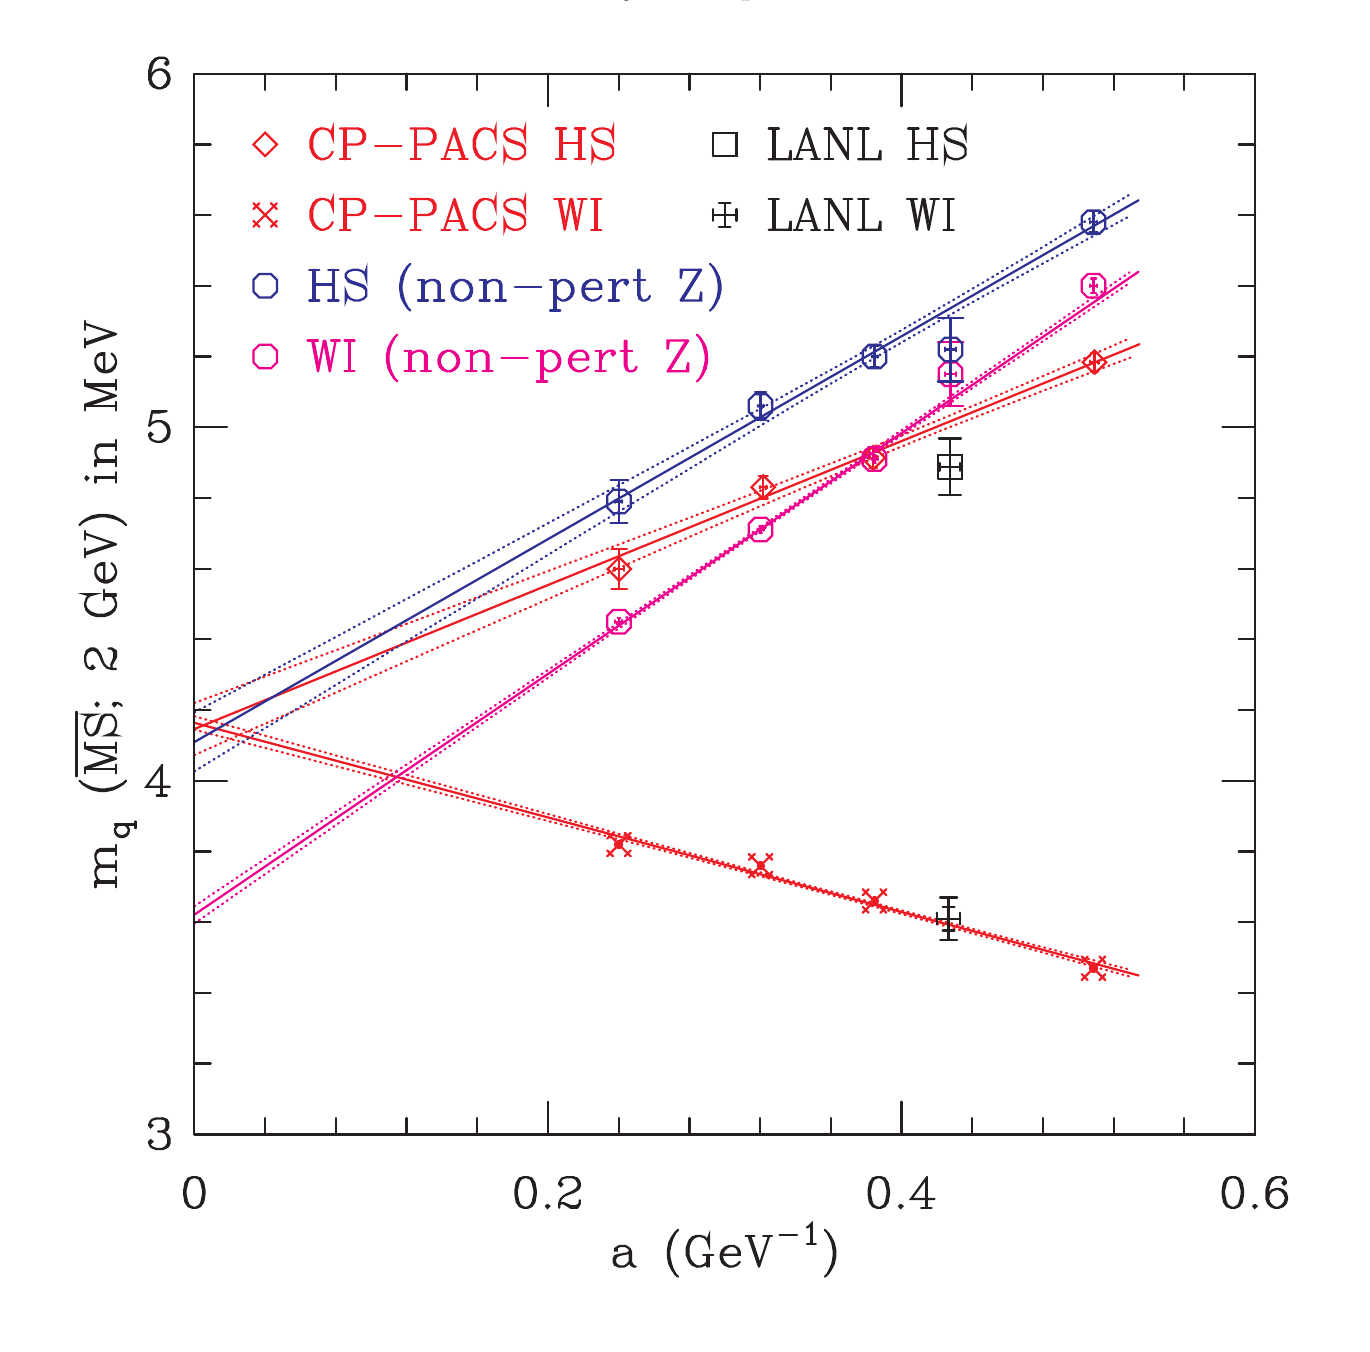
\includegraphics[width=0.8\textwidth]{images/fig35.png}
\caption{The behavior of $m = (m_u + m_d)/2$ as a function of the lattice spacing $a$ for Wilson fermions. Data from the hadron spectroscopy and Ward Identity method are shown for two ways of estimating the renormalization constants, i.e.\ one loop perturbative and non-perturbative.}
\label{fig:35}
\end{figure}

The recent non-perturbative calculations of the $Z$'s [186] challenge this nice picture. Fig.~\ref{fig:35} also shows the same data analyzed using these non-perturbative $Z$'s. At fixed $a$ the non-perturbative $Z$'s increase both the hadron spectroscopy and WI results to roughly the same value. This suggests that most of the difference is due to the $O(\alpha_s^2)$ corrections to the 1-loop $Z$'s and not due to the $O(a)$ discretization errors as mentioned before. However, the non-perturbative calculation of $Z$'s themselves have $O(a)$ errors that have not been resolved in the results of [186]. As a result we do not have a clear separation between the effects of the $O(a)$ discretization errors and the $O(\alpha_s^2)$ errors in these $Z$'s.

The bottom line is that, even though we have not resolved the two kinds of errors, and while both the value at fixed $a$ and the slope in $a$ increases significantly on changing from 1-loop to non-perturbative $Z$'s, the extrapolated value is roughly unchanged.

To conclude, I believe that we have finally obtained values for light quark masses with reliable estimates of statistical and all systematic errors other than quenching. Calculations are already underway to significantly increase the number of data points with $n_f = 2$ and 4 flavors of dynamical quarks to reduce the quenching uncertainty. Also, new ways to calculate the renormalization constants non-perturbatively are being developed. Therefore, I expect that in the next few years there will be a significant increase in the precision of both QQCD and full QCD estimates of light quark masses.

\section{Schr\"odinger Functional Approach}

In the above discussion the term non-perturbative $Z$'s referred to only the lattice scheme. In the required matching constants one still has to use perturbative expressions for the renormalization constants in the continuum scheme and make a good estimate of the matching point. The ALPHA Collaboration has proposed a method for removing this last vestige of dependence on perturbation theory [187]. The details of their method have been discussed by Prof.~L\"uscher at this school, so I will just summarize the key points.
\begin{enumerate}
\item[(i)] Calculate the quark mass using the axial WI method at some infrared lattice scale. At the same time calculate $Z_P$ and $Z_A$ non-perturbatively in the Schr\"odinger functional scheme.
\item[(ii)] Evolve this lattice result to some very high scale using the step scaling function calculated non-perturbatively.
\item[(iii)] At this high scale, where $\alpha_s$ is small, define the renormalization group independent mass
\begin{equation}
\hat{m} = \lim_{a\to 0} m_R \left[2\beta_0 g^2\right]^{-\gamma_0/2\beta_0}.
\end{equation}
\end{enumerate}
This $\hat{m}$ is scheme independent, thus subsequent conversion to a running mass in some scheme and at some desired scale can be done in the continuum using the most accurate versions (4-loop) of the scale evolution equations [188]. To reiterate, the advantage of this method is that the lattice calculations directly predict the scale and scheme invariant quantity $\hat{m}$. The calculations by the ALPHA Collaboration are still in progress and at this time estimates for $\hat{m}$ have not been released. It will be interesting to see how they compare with conventional hadron spectroscopy or WI methods discussed above. My prejudice is that they will be very similar.

\section{Role of quark masses in CP violation}

A very opportune application of the precise determination of the light quark masses is in the Standard Model prediction of direct CP violation in kaon decays characterized by the ratio $\epsilon'/\epsilon$ (see lectures by Prof.~Buras and [189]). The reason is that $\epsilon'/\epsilon$ is, to a good approximation, proportional to $1/(m_d + m_s)^2$ [190],
\begin{equation}
\epsilon'/\epsilon = A \left[c_0 + c_6 B_6^{3/2} + c_8 B_8^{3/2}\right] \left(\frac{158~\mathrm{MeV}}{m_s + m_d}\right)^2,
\end{equation}
where all quantities are to be evaluated at the scale $m_c = 1.3$~GeV. Eq.~20.5 highlights the dependence on the light quark masses and the bag parameters $B_6^{3/2}$ and $B_8^{3/2}$ which LQCD is also expected to provide. The coefficients $c_0$, $c_6$, and $c_8$ have been calculated to next-to-next-to-leading order, and with $M_{top}$ now known the main uncertainty in their extraction comes from the value of $\Lambda_{QCD}$. The quantity $A = |V_{ub}||V_{cb}| \sin\delta$ in the parameterization of Eq.~2.4, requires input of other SM parameters like $f_B$, $|V_{ub}|$, $|V_{cb}|$, $B_K$, $B_{B_d} f_{B_d}$. Using the central values quoted by Buras at scale $m_c = 1.3$~GeV [190] one gets $A = 1.29 \times 10^{-4}$, $c_0 = -1.4$, $c_6 = 7.9$, $c_8 = -4.0$. Unfortunately, the errors in these quantities make the resulting theoretical prediction, $\epsilon'/\epsilon = 3.6(3.4) \times 10^{-4}$ [190], very loose.

Current experimental estimates are $7.4(5.9) \times 10^{-4}$ from Fermilab E731 [191] and $23(7) \times 10^{-4}$ from CERN NA31 [192]. The new generation of experiments, Fermilab E832, CERN NA48, and DA$\Phi$NE KLOE, will reduce the uncertainty to $\approx 1 \times 10^{-4}$. First results from these experiments (see lectures by L.~Fayard) should be available in the next couple of years. Thus, it is very important to tighten the theoretical prediction. Clearly, lower estimates of quark masses suggested by LQCD would significantly increase the size of direct CP violation, and make its experimental determination and validation much easier.

\section{Heavy quark masses $m_c$ and $m_b$}

The masses of the heavy quarks, $m_c$ and $m_b$, have been calculated using the charmonium and upsilon spectroscopy. For heavy quarks there exist two different definitions of the quark mass --- the pole and $\overline{\mathrm{MS}}$ masses. The pole mass is defined to be $m^{(pole)} = (M_{onia} - E_{binding})/2$, where $M_{onia}$ is taken from experimental data and $E_{binding}$ is calculated on the lattice. This calculation has been done using two approaches, NRQCD [193] and heavy quark effective theory (HQET) [194], and the results are consistent. The $\overline{\mathrm{MS}}$ mass, which has the advantage of being free of renormalon ambiguities that are inherent in $m^{(pole)}$, is obtained from $m^{(pole)}$ using perturbation theory. The present results are
\begin{equation}
\begin{aligned}
m_b^{\overline{\mathrm{MS}}} &= 4.15(5)(20)~\mathrm{GeV} && \text{(APE)}, \\
m_b^{\overline{\mathrm{MS}}} &= 4.16(15)~\mathrm{GeV} && \text{(NRQCD)}.
\end{aligned}
\end{equation}
These estimates are consistent with determinations from other non-lattice methods.

The agreement is not as good for various lattice estimates of $m_c^{\overline{\mathrm{MS}}}$. Current estimates lie between $1.2 - 1.5$~GeV. For example, three different methods investigated by the APE collaboration [195,186], Fermilab collaboration [196,197], and by Bochkarev and Forcrand [198] who evaluate the correlation functions arising in QCD sum-rules on the lattice, give
\begin{equation}
\begin{aligned}
m_c^{\overline{\mathrm{MS}}} &= 1.525(40)(125)~\mathrm{GeV} && \text{(APE)}, \\
m_c^{\overline{\mathrm{MS}}} &= 1.33(8)~\mathrm{GeV} && \text{(Fermilab)}, \\
m_c^{\overline{\mathrm{MS}}} &= 1.22(5)~\mathrm{GeV} && \text{(B\&F)}.
\end{aligned}
\end{equation}
At this stage I do not consider the difference significant as the various systematic errors have not been resolved equally well in all the calculations.

\section*{Conclusions and Acknowledgements}

I hope that these lectures succeed in providing a pedagogical introduction to Lattice QCD, and to the analyses of numerical data. Undoubtedly, some topics have been left out and many are sketchy. My purpose was to give a broad overview. I have concentrated on providing the basics and have illustrated the analyses of Monte Carlo data by the calculations of the hadron spectrum, strong coupling constant $\alpha_s$, and quark masses. Prof.~Martinelli will, among other things, discuss the extraction of matrix elements of weak Hamiltonian, while Prof.~L\"uscher will provide a panoramic view of what future calculations will look like and the improvement possible with better discretization schemes. Together, I hope these set of lectures provide sufficient details and excitement to motivate some of you to probe deeper into the field.

I express my gratitude to all the lecturers, students, and staff who made this Les Houches school fun and exciting. It, most certainly, was a memorable six weeks for me. In preparing these lectures I would like to thank G.~Bali, U.~Heller, C.~Michael, M.~Peardon, the CP-PACS collaboration, in particular S.~Hashimoto and T.~Yoshie, for providing unpublished data. Special thanks go to my collaborators T.~Bhattacharya, D.~Daniel, G.~Kilcup, A.~Patel, and S.~Sharpe from whom I have, over the years, learned so much. Finally, I would like to thank T.~Bhattacharya, D.~Daniel, W.~Lee, and S.~Sharpe for proof reading these notes and for their suggestions.


\chapter*{References}
\addcontentsline{toc}{chapter}{References}

\begin{enumerate}
\renewcommand{\labelenumi}{[\arabic{enumi}]}
\item M.~Creutz, \textit{Quarks, Gluons, and Lattices}, Cambridge University Press, 1983.
\item \textit{Quantum Fields on the Computer}, Ed.~M.~Creutz, World Scientific, 1992.
\item I.~Montvay and G.~M\"unster, \textit{Quantum Fields on a Lattice}, Cambridge University Press, 1994.
\item H.~J.~Rothe, \textit{Quantum Gauge Theories: An Introduction}, World Scientific, 1997.
\item \textit{Phenomenology and Lattice QCD}, Eds.~G.~Kilcup and S.~Sharpe, World Scientific, 1995.
\item \textit{1989 TASI Lectures}, Eds.~T.~Degrand and D.~Toussaint, World Scientific, 1990.
\item J.~Kogut, Rev.\ Mod.\ Phys.\ 51 (1979) 659.
\item J.~Kogut, Rev.\ Mod.\ Phys.\ 55 (1983) 775.
\item LATTICE93 Nucl.\ Phys.\ (Proc.\ Suppl.)\ B34 (1994) 1; LATTICE94 Nucl.\ Phys.\ (Proc.\ Suppl.)\ B42 (1995) 1; LATTICE95 Nucl.\ Phys.\ (Proc.\ Suppl.)\ B47 (1996) 1; LATTICE96 Nucl.\ Phys.\ (Proc.\ Suppl.)\ B53 (1997) 1; LATTICE97 Nucl.\ Phys.\ (Proc.\ Suppl.)\ B63 (1998) 1.
\item A.~Buras, hep-ph/9711217; these proceedings.
\item J.~Richman, these proceedings.
\item P.~van Baal, Nucl.\ Phys.\ (Proc.\ Suppl.)\ B63 (1998) 126.
\item C.~Detar, To appear in `Quark Gluon Plasma 2', edited by R.~Hwa, World Scientific, 1998 (hep-ph/9504325); A.~Ukawa, Lectures at INT, Published in Ref.~[5]. J-P.~Blaizot, J.~Korean Physical Society 25 (1992) S65-S98; J.~Kapusta, \textit{Finite Temperature Field Theory}, Cambridge University Press, 1989.
\item H.~B.~Nielsen and M.~Ninomiya, Nucl.\ Phys.\ B185 (1981) 20; Erratum Nucl.\ Phys.\ B195 (1982) 541; Nucl.\ Phys.\ B193 (1981) 173.
\item Y.~Shamir, Nucl.\ Phys.\ (Proc.\ Suppl.)\ B53 (1997) 664; Nucl.\ Phys.\ (Proc.\ Suppl.)\ B47 (1996) 212.
\item R.~Narayanan, hep-lat/9707035.
\item M.~Testa, hep-lat/9707007.
\item P.~Hasenfratz, hep-lat/9802007; M.~L\"uscher, hep-lat/9802011.
\item K.~G.~Wilson, Phys.\ Rev.\ D10 (1974) 2445; in \textit{New Phenomena in Subnuclear Physics} (Erice 1975), Ed.~A.~Zichichi, Plenum New York, 1977.
\item B.~Sheikholesalami and R.~Wohlert, Nucl.\ Phys.\ B259 (1985) 572.
\item J.~Kogut and L.~Susskind, Phys.\ Rev.\ D11 (1975) 395; T.~Banks, J.~Kogut, and L.~Susskind, Phys.\ Rev.\ D13 (1996) 1043; L.~Susskind, Phys.\ Rev.\ D16 (1977) 3031.
\item G.~Parisi, \textit{Statistical Field Theory}, Benjamin/Cummings, 1988.
\item J.~Zinn-Justin, \textit{Quantum Field Theory and Critical Phenomena}, Oxford University Press, Oxford, 1993.
\item K.~Osterwalder and R.~Schrader, Comm.\ Math.\ Phys.\ 31 (1973) 83; Comm.\ Math.\ Phys.\ 42 (1975) 281.
\item M.~L\"uscher, Comm.\ Math.\ Phys.\ 54 (1977) 283.
\item C.~Michael, Nucl.\ Phys.\ B327 (1990) 515; T.~DeGrand, Phys.\ Rev.\ D43 (1991) 2296.
\item M.~L\"uscher, \textit{Selected Topics In Lattice Field Theory}, Lectures at the 1988 Les Houches Summer School, North Holland, 1990.
\item M.~L\"uscher, Comm.\ Math.\ Phys.\ 104 (1977) 177; Comm.\ Math.\ Phys.\ 105 (1986) 153; Nucl.\ Phys.\ B354 (1991) 531; Nucl.\ Phys.\ B364 (1991) 237.
\item S.~Sharpe, R.~Gupta, and G.~Kilcup, Nucl.\ Phys.\ B383 (1992) 309; R.~Gupta, A.~Patel, and S.~Sharpe, Phys.\ Rev.\ D48 (1993) 388;
\item M.~Fukugita, Y.~Kuramashi, H.~Mino, M.~Okawa, and A.~Ukawa, Phys.\ Rev.\ D52 (1995) 3003.
\item K.~Wilson, Phys.\ Rev.\ D10 (1974) 2445.
\item R.~Celmaster, Phys.\ Rev.\ D26 (1982) 2955.
\item N.~H.~Christ, R.~Friedberg, and T.~D.~Lee, Nucl.\ Phys.\ B202 (1982) 89; Nucl.\ Phys.\ B210 (1982) 310, 337.
\item J.~Mandula, G.~Zweig, J.~Goverts, Nucl.\ Phys.\ B228 (1983) 91, 109.
\item G.~P.~Lepage, hep-lat/9607076.
\item H.~Kawai, R.~Nakayama, and K.~Seo, Nucl.\ Phys.\ B189 (1981) 40.
\item S.~Elitzur, Phys.\ Rev.\ D12 (1975) 3978.
\item D.~Leinweber, et.\ al., hep-lat/9803015.
\item C.~Parrinello, et.\ al., Nucl.\ Phys.\ (Proc.\ Suppl.)\ B63 (1998) 245.
\item R.~Gupta, D.~Daniel and J.~Grandy, Phys.\ Rev.\ D48 (1993) 3330.
\item V.~Gim\'enez, et.\ al., hep-lat/9806006.
\item V.~N.~Gribov, Nucl.\ Phys.\ B139 (1978) 1.
\item P.~van Baal, hep-th/9711070.
\item A.~Cucchieri and T.~Mendes, Nucl.\ Phys.\ (Proc.\ Suppl.)\ B53 (1997) 811.
\item J.~Hetrick and Ph.~de Forcrand, Nucl.\ Phys.\ (Proc.\ Suppl.)\ B63 (1998) 838.
\item M.~C.~Paciello, et.\ al., Phys.\ Lett.\ 289B (1992) 405; Ph.~de Forcrand and J.~Hetrick, Nucl.\ Phys.\ (Proc.\ Suppl.)\ B42 (1995) 861; A.~Cucchieri, Nucl.\ Phys.\ B508 (1997) 353.
\item G.~Martinelli, et.\ al., Phys.\ Lett.\ 411B (1997) 141.
\item L.~Maiani and M.~Testa, Phys.\ Lett.\ 245B (1990) 585.
\item K.~Symanzik, Nucl.\ Phys.\ B226 (1983) 187 and 205.
\item M.~L\"uscher, Comm.\ Math.\ Phys.\ 85 (1982) 39.
\item J.~Grandy and R.~Gupta, Nucl.\ Phys.\ (Proc.\ Suppl.)\ B42 (1995) 246; J.~Grandy and G.~Kilcup, Nucl.\ Phys.\ (Proc.\ Suppl.)\ B53 (1997) 560.
\item T.~DeGrand, A.~Hasenfratz, and T.~Kovacs, hep-lat/9801037.
\item P.~Hasenfratz, hep-lat/9802007.
\item P.~Ginsparg and K.~W.~Wilson, Phys.\ Rev.\ D25 (1982) 2649.
\item M.~L\"uscher, hep-lat/9802011.
\item K.~G.~Wilson, in \textit{New Phenomena in Subnuclear Physics}, ed.~A.~Zichichi (Plenum Press, 1977).
\item M.~Bochicchio, L.~Maiani, G.~Martinelli, G.~C.~Rossi and M.~Testa, Nucl.\ Phys.\ B262 (1985) 331; Phys.\ Lett.\ 176B (1986) 445; Phys.\ Lett.\ 178B (1986) 265; Phys.\ Lett.\ 181B (1986) 344; Nucl.\ Phys.\ B289 (1987) 505; and Nucl.\ Phys.\ B293 (1987) 420.
\item Karsten and J.~Smit, Nucl.\ Phys.\ B183 (1981) 103.
\item W.~Bardeen, et.\ al., Phys.\ Rev.\ D57 (1998) 1633.
\item A.~Duncan, E.~Eichten, and H.~Thacker, hep-lat/9806020.
\item M.~Gell-Mann, R.~J.~Oakes, and B.~Renner, Phys.\ Rev.\ 175 (1968) 2195.
\item D.~Daniel, R.~Gupta, G.~Kilcup, A.~Patel, and S.~Sharpe, Phys.\ Rev.\ D46 (1992) 3130.
\item G.~Kilcup and S.~Sharpe, Nucl.\ Phys.\ B283 (1987) 493.
\item H.~S.~Sharatchandra, H.~J.~Thun, and P.~Weisz, Nucl.\ Phys.\ B192 (1981) 205; C.~van den Doel and J.~Smit, Nucl.\ Phys.\ B228 (1983) 122; M.~Golterman and J.~Smit, Nucl.\ Phys.\ B245 (1984) 61.
\item H.~Kluberg-Stern, A.~Morel, O.~Napoly, and B.~Petersson, Nucl.\ Phys.\ B220 (1983) 447.
\item F.~Gliozzi, Nucl.\ Phys.\ B204 (1982) 419.
\item D.~Daniel, and T.~D.~Kieu, Phys.\ Lett.\ 175B (1986) 73.
\item M.~Golterman, Nucl.\ Phys.\ B273 (1986) 663.
\item R.~Gupta, G.~Guralnik, G.~Kilcup, and S.~Sharpe, Phys.\ Rev.\ D43 (1991) 2003.
\item M.~Golterman and J.~Smit, Nucl.\ Phys.\ B255 (1985) 328.
\item S.~Sharpe \textit{Standard Model Phenomenology and Weak Decay on the lattice}, Ed.~G.~Martinelli, World Scientific, 1998.
\item G.~Kilcup, et.\ al., Phys.\ Rev.\ Lett.\ 64 (1990) 25; G.~Kilcup, R.~Gupta, and S.~Sharpe, Phys.\ Rev.\ D57 (1998) 1654;
\item M.~L\"uscher and P.~Weisz, Commun.\ Math.\ Phys.\ 97 (1985) 59; Erratum Commun.\ Math.\ Phys.\ 98 (1985) 433.
\item G.~Curci, P.~Menotti and G.~Paffuti, Phys.\ Lett.\ 130B (1983) 205.
\item P.~Weisz and R.~Wohlert, Nucl.\ Phys.\ B236 (1984) 397.
\item M.~L\"uscher and P.~Weisz, Phys.\ Lett.\ 158B (1985) 250.
\item G.~Parisi, High Energy Physics - 1980, AIP Conference Proceedings No.~68, Eds.~L.~Durand and L.~Pondrom, New York, 1981.
\item P.~Lepage and P.~Mackenzie, Phys.\ Rev.\ D48 (1993) 2250.
\item M.~Alford, T.~Klassen, and P.~Lepage, hep-lat/9712005.
\item P.~Weisz and R.~Wohlert, Nucl.\ Phys.\ B236 (1984) 397.
\item M.~Alford, et.\ al., Nucl.\ Phys.\ (Proc.\ Suppl.)\ B42 (1994) 787.
\item M.~Alford, et.\ al., Phys.\ Lett.\ 361B (1995) 87.
\item K.~Wilson and J.~Kogut, Phys.\ Rev.\ 12 (1974) 76.
\item K.~Wilson, in \textit{Recent Developments in Gauge Theories}, edited by G.~'t Hooft, et.\ al., Plenum Press, N.Y. 1980.
\item M.~Fisher, Lecture notes in Physics, Vol.~186, Springer Verlag, 1983.
\item R.~Gupta, in proceedings of LATTICE 85, Wuppertal 1985, Eds.~K-H M\"utter and K.~Schilling, Plenum Press (1986).
\item A.~Patel and R.~Gupta, Phys.\ Lett.\ 183B (1987) 193.
\item R.~Gupta, lectures at TASI 89 [6].
\item R.~Gupta, in \textit{Quantum Fields on the Computer}, Ed.~M.~Creutz, World Scientific, 1992.
\item P.~Hasenfratz, hep-lat/9803027.
\item Y.~Iwasaki, University of Tsukuba report UTHEP-118, 1983.
\item K.~Kanaya, hep-lat/9804006.
\item R.~Gupta, et.\ al., Phys.\ Rev.\ D43 (1991) 2301.
\item QCDTARO Collaboration, Nucl.\ Phys.\ (Proc.\ Suppl.)\ B53 (1997) 938.
\item QCDTARO Collaboration, Nucl.\ Phys.\ (Proc.\ Suppl.)\ B63 (1997) 928; hep-lat/9806008.
\item P.~Hasenfratz and F.~Niedermayer, Nucl.\ Phys.\ B414 (1994) 785.
\item P.~Hasenfratz, Nucl.\ Phys.\ (Proc.\ Suppl.)\ B63 (1998) 53.
\item R.~Swendsen, Phys.\ Rev.\ Lett.\ 47 (1981) 1775.
\item T.~DeGrand, A.~Hasenfratz, P.~Hasenfratz, F.~Niedermayer, Phys.\ Lett.\ 365B (1996) 233.
\item T.~DeGrand, Nucl.\ Phys.\ (Proc.\ Suppl.)\ B63 (1998) 913, and hep-lat/9802012.
\item F.~Farchioni and A.~Papa, Nucl.\ Phys.\ (Proc.\ Suppl.)\ B63 (1998) 910.
\item H.~Hamber and C.~M.~Wu, Phys.\ Lett.\ 133B (1983) 351.
\item R.~Wohlert, DESY 87/069; M.~L\"uscher and P.~Weisz, Nucl.\ Phys.\ B479 (1996) 429.
\item M.~L\"uscher, ALPHA Collaboration, Nucl.\ Phys.\ B478 (1996) 365.
\item R.~Edwards, U.~Heller, and T.~Klassen, hep-lat/9711052.
\item G.~Martinelli, C.~T.~Sachrajda and A.~Vladikas, Nucl.\ Phys.\ B358 (1991) 212.
\item M.~Alford, T.~Klassen, and P.~Lepage, Nucl.\ Phys.\ B496 (1997) 377.
\item P.~Lepage and B.~Thacker, Phys.\ Rev.\ D43 (1991) 196; G.~Lepage, L.~Magnea, C.~Nakhleh, U.~Magnea and K.~Hornbostel, Phys.\ Rev.\ D46 (1992) 4052.
\item A.~Ali Khan, et.\ al., hep-lat/9801038.
\item C.~T.~H.~Davies, et.\ al., Phys.\ Rev.\ D56 (1997) 2755.
\item C.~T.~H.~Davies, et.\ al., hep-lat/9802024; C.~T.~H.~Davies, Nucl.\ Phys.\ (Proc.\ Suppl.)\ B60A (1998) 124; hep-lat/9705039.
\item W.~Bietenholz, R.~Brower, S.~Chandrasekharan, and U.-J.~Wiese, Nucl.\ Phys.\ (Proc.\ Suppl.)\ B53 (1997) 921.
\item A.~X.~El-Khadra, A.~S.~Kronfeld, P.~B.~Mackenzie, Phys.\ Rev.\ D55 (1997) 3933.
\item D.~Kaplan, Phys.\ Lett.\ 288B (1992) 342; Y.~Shamir, Nucl.\ Phys.\ B406 (1993) 90.
\item T.~Blum and A.~Soni, hep-lat/9712004.
\item G.~'t Hooft, Comments at the 1972 Marseilles Conference, Unpublished; H.~D.~Politzer, Phys.\ Rev.\ Lett.\ 30 (1973) 1346; D.~Gross and F.~Wilczek, Phys.\ Rev.\ Lett.\ 30 (1973) 1343.
\item W.~Celmaster and R.~J.~Gonsalves, Phys.\ Rev.\ D20 (1979) 1420.
\item G.~S.~Bali and K.~Schilling, Phys.\ Rev.\ D47 (1993) 661; G.~S.~Bali and K.~Schilling, Int.\ J.\ Mod.\ Phys.\ C4 (1993) 1167.
\item G.~S.~Bali et al.\ (T$\chi$L collab), Nucl.\ Phys.\ (Proc.\ Suppl.)\ B63 (1998) 209; G.~S.~Bali, et.\ al., (T$\chi$L collab), in preparation; U.~Gl\"assner, et.\ al., (SESAM Collab.)\ PLB383 (1997) 98.
\item M.~Creutz, Phys.\ Rev.\ D21 (1980) 2308.
\item H.~Wittig, et.\ al., UKQCD collaboration, Nucl.\ Phys.\ (Proc.\ Suppl.)\ B42 (1995) 288.
\item M.~Guagnelli, R.~Sommer, and H.~Wittig, hep-lat/9806005.
\item A.~Yu.~Dublin, A.~Kaidalov, and Yu.~A.~Simonov, Phys.\ Lett.\ 323B (1994) 41.
\item W.~Lucha, F.~Sch\"oberl, and D.~Gromes, Phys.\ Rev.\ 200 (1991) 128.
\item L.~Burakovsky, hep-ph/9805286.
\item S.~Veseli and M.~Olsson, Phys.\ Lett.\ 383B (1996) 109.
\item R.~Sommer, Nucl.\ Phys.\ B411 (1994) 839.
\item B.~Svetitsky and L.~Yaffe, Nucl.\ Phys.\ B210 (1982) 423; B.~Svetitsky, Phys.\ Rev.\ 132 (1986) 1,
\item J.~Engels, S.~Mashkevich, T.~Scheideler, and G.~Zinovev, Phys.\ Lett.\ 365B (1996) 219; G.~Boyd, et.\ al., Nucl.\ Phys.\ B469 (1996) 419.
\item A.~Guth, Phys.\ Rev.\ D21 (1980) 2291; J.~Fr\"ohlich and T.~Spencer, Comm.\ Math.\ Phys.\ 83 (1982) 411.
\item M.~Creutz, L.~Jacobs, and C.~Rebbi, Phys.\ Rev.\ D20 (1979) 1915; T.~Degrand and D.~Toussaint, Phys.\ Rev.\ D22 (1980) 2478.
\item M.~Creutz, Phys.\ Rev.\ Lett.\ 43 (1979) 553; M.~Creutz, L.~Jacobs, and C.~Rebbi, Phys.\ Rev.\ Lett.\ 42 (1979) 1390.
\item G.~M\"unster and P.~Weisz, Phys.\ Lett.\ 119B (1980) 119.
\item U.~Heller and F.~Karsch, Nucl.\ Phys.\ B251 [FS13] (1985) 254; and private communications.
\item G.~Bhanot and M.~Creutz, Phys.\ Rev.\ D24 (1981) 3212.
\item R.~Gavai, Nucl.\ Phys.\ B474 (1996) 446.
\item U.~Heller, Phys.\ Lett.\ 362B (1995) 123.
\item K.~Moriarty, Phys.\ Lett.\ 106B (1981) 130; G.~G.~Batrouni and B.~Svetitsky, Phys.\ Rev.\ Lett.\ 52 (1984) 2205; Y.~Makeenko and M.~Polikarpov, Nucl.\ Phys.\ B205 (1982) 386.
\item C.~Morningstar and M.~Peardon, in preparation.
\item A.~Patrascioiu and E.~Seiler, Phys.\ Rev.\ D57 (1998) 1394.
\item S.~Duane, A.~D.~Kennedy, B.~Pendleton, D.~Roweth, Phys.\ Lett.\ 195B (1987) 216.
\item B.~All\`es, et.\ al., hep-lat/9803008.
\item S.~Aoki, et.\ al., Phys.\ Rev.\ D50 (1994) 486.
\item A.~Duncan, E.~Eichten, and E.~Eichten, Phys.\ Rev.\ Lett.\ 76 (1996) 3894.
\item E.~Eichten and B.~Hill, Phys.\ Lett.\ 243B (1990) 427, Phys.\ Lett.\ 240B (1990) 193; Phys.\ Lett.\ 234B (1990) 511. M.~Neubert, Phys.\ Rev.\ 245 (1994) 259; G.~Martinelli and C.~Sachrajda, Nucl.\ Phys.\ B478 (1996) 660; J.~Mandula and M.~Ogilvie, Phys.\ Rev.\ D57 (1998) 1397.
\item M.~L\"uscher, et.\ al., ALPHA Collaboration, hep-lat/9611015.
\item A.~Donini, et.\ al., Nucl.\ Phys.\ (Proc.\ Suppl.)\ B53 (1997) 883; G.~Martinelli, et.\ al., Phys.\ Lett.\ 411B (1997) 141.
\item G.~M.~de Divitiis and R.~Petronzio, Phys.\ Lett.\ 419B (1998) 311.
\item E.~Witten, Nucl.\ Phys.\ B156 (1979) 269; G.~Veneziano, Nucl.\ Phys.\ B159 (1979) 213.
\item S.~Sharpe, Phys.\ Rev.\ D46 (1992) 3146; J.~Labrenz and S.~Sharpe, Phys.\ Rev.\ D54 (1996) 4595; S.~Sharpe and Y.~Zhang Phys.\ Rev.\ D53 (1996) 5125.
\item C.~Bernard and M.~Golterman, Phys.\ Rev.\ D46 (1992) 853; M.~Golterman, hep-lat/9405002 and hep-lat/9411005.
\item J.~Gasser and H.~Leutwyler, Nucl.\ Phys.\ B250 (1985) 465.
\item R.~Gupta, Nucl.\ Phys.\ (Proc.\ Suppl.)\ B42 (1995) 85;
\item S.~Sharpe, Nucl.\ Phys.\ (Proc.\ Suppl.)\ B53 (1997) 181.
\item G.~Kilcup, S.~Sharpe, R.~Gupta, and A.~Patel Phys.\ Rev.\ Lett.\ 64 (1990) 25; G.~Kilcup, R.~Gupta, and S.~Sharpe, Phys.\ Rev.\ D57 (1998) 1654.
\item T.~Bhattacharya, R.~Gupta, G.~Kilcup, and S.~Sharpe, Phys.\ Rev.\ D53 (1996) 6486.
\item C.~Bernard, T.~Draper, A.~Soni, D.~Politzer and M.~Wise, Phys.\ Rev.\ D32 (1985) 2343.
\item S.~Aoki, et.\ al., JLQCD Collaboration, Nucl.\ Phys.\ (Proc.\ Suppl.)\ B47 (1996) 354.
\item P.~Lepage, 1989 TASI Lectures, Eds.~T.~Degrand and D.~Toussaint, World Scientific, 1990.
\item S.~Gottlieb, Nucl.\ Phys.\ (Proc.\ Suppl.)\ B53 (1997) 155.
\item T.~Yoshie, Nucl.\ Phys.\ (Proc.\ Suppl.)\ B63 (1998) 3; hep-lat/9711017.
\item T.~Bhattacharya, et.\ al., in preparation.
\item J.~Flynn, Nucl.\ Phys.\ (Proc.\ Suppl.)\ B53, (1997) 168.
\item T.~Onogi, Nucl.\ Phys.\ (Proc.\ Suppl.)\ B63A-C, (1998) 59; A.~Ali Khan, Nucl.\ Phys.\ (Proc.\ Suppl.)\ B63A-C, (1998) 71; Y.~Yoshie, Nucl.\ Phys.\ (Proc.\ Suppl.)\ B63A-C, (1998) 3.
\item T.~Barnett and S.~Sharpe, Ann.\ Rev.\ Nuc.\ Part.\ Sci.\ 40 (1990) 327.
\item R.~Gupta, A.~Patel, C.~Baillie, G.~Kilcup, S.~Sharpe, Phys.\ Rev.\ D43 (1991) 2301.
\item C.~Michael and M.~Teper, Nucl.\ Phys.\ B314 (1989) 347.
\item G.~Bali and K.~Schilling, Phys.\ Lett.\ 309B (1993) 378.
\item H.~Chen et.\ al., Nucl.\ Phys.\ (Proc.\ Suppl.)\ B34 (1994) 357.
\item C.~Michael, hep-ph/9710502.
\item W.~Lee and D.~Weingarten, hep-lat/9805029.
\item C.~Morningstar and M.~Peardon, Phys.\ Rev.\ D56 (1997) 4043.
\item M.~Peardon, Nucl.\ Phys.\ (Proc.\ Suppl.)\ B63 (1998) 22.
\item P.~Lacock, et.\ al., Phys.\ Lett.\ 401B (1997) 308.
\item T.~Manke, et al, Nucl.\ Phys.\ (Proc.\ Suppl.)\ B63 (1998) 332.
\item S.~Collins, Nucl.\ Phys.\ (Proc.\ Suppl.)\ B63 (1998) 335.
\item D.~Weingarten, Phys.\ Rev.\ Lett.\ 51 (1983) 1830.
\item S.~Nussinov, Phys.\ Rev.\ Lett.\ 51 (1983) 2081.
\item E.~Witten, Phys.\ Rev.\ Lett.\ 51 (1983) 2351.
\item C.~Vafa and E.~Witten, Phys.\ Rev.\ Lett.\ 51 (1983) 2351.
\item G.~West, Phys.\ Rev.\ Lett.\ 77 (1996) 2622.
\item S.~Capitani, et.\ al., Nucl.\ Phys.\ (Proc.\ Suppl.)\ B63A-C (1998) 153.
\item R.~Gupta and T.~Bhattacharya, Phys.\ Rev.\ D55 (1997) 7203.
\item B.~Gough, et.\ al., Phys.\ Rev.\ Lett.\ 79 (1997) 1622.
\item T.~Bhattacharya and R.~Gupta, Nucl.\ Phys.\ (Proc.\ Suppl.)\ B63A-C (1998) 95.
\item V.~Gimenez, et.\ al., hep-lat/9801028.
\item S.~Capitani et.\ al., Nucl.\ Phys.\ (Proc.\ Suppl.)\ B63 (1998) 153.
\item J.~A.~M.~Vermaseren et.\ al., Phys.\ Lett.\ 405B (1997) 327.
\item A.~Buras, hep-ph/9610461.
\item A.~Buras, M.~Jamin, and M.~E.~Lautenbacher, Phys.\ Lett.\ 389B (1996) 749.
\item L.~K.~Gibbons, et.\ al., Phys.\ Rev.\ Lett.\ 70 (1993) 1203.
\item G.~D.~Barr, et.\ al., Phys.\ Lett.\ 317B (1993) 233.
\item C.~T.~H.~Davies, et.\ al., Phys.\ Rev.\ Lett.\ 73 (1994) 2654.
\item V.~Gimenez, G.~Martinelli, and C.~Sachrajda, Phys.\ Lett.\ 393B (1997) 124.
\item C.~Allton, et.\ al., Nucl.\ Phys.\ B431 (1994) 667.
\item A.~El-Khadra, hep-lat/9509381.
\item A.~Kronfeld, Nucl.\ Phys.\ (Proc.\ Suppl.)\ B63 (1998) 311.
\item A.~Bochkarev, P.~de Forcrand, Nucl.\ Phys.\ B477 (1996) 489; Nucl.\ Phys.\ (Proc.\ Suppl.)\ B53 (1997) 305.
\end{enumerate}


\end{document}
